\documentclass[]{book}
\usepackage{lmodern}
\usepackage{amssymb,amsmath}
\usepackage{ifxetex,ifluatex}
\usepackage{fixltx2e} % provides \textsubscript
\ifnum 0\ifxetex 1\fi\ifluatex 1\fi=0 % if pdftex
  \usepackage[T1]{fontenc}
  \usepackage[utf8]{inputenc}
\else % if luatex or xelatex
  \ifxetex
    \usepackage{mathspec}
  \else
    \usepackage{fontspec}
  \fi
  \defaultfontfeatures{Ligatures=TeX,Scale=MatchLowercase}
\fi
% use upquote if available, for straight quotes in verbatim environments
\IfFileExists{upquote.sty}{\usepackage{upquote}}{}
% use microtype if available
\IfFileExists{microtype.sty}{%
\usepackage{microtype}
\UseMicrotypeSet[protrusion]{basicmath} % disable protrusion for tt fonts
}{}
\usepackage[margin=1in]{geometry}
\usepackage{hyperref}
\hypersetup{unicode=true,
            pdftitle={Introduction to Econometrics with R},
            pdfauthor={Florian Oswald, Jean-Marc Robin and Vincent Viers},
            pdfborder={0 0 0},
            breaklinks=true}
\urlstyle{same}  % don't use monospace font for urls
\usepackage{natbib}
\bibliographystyle{apalike}
\usepackage{color}
\usepackage{fancyvrb}
\newcommand{\VerbBar}{|}
\newcommand{\VERB}{\Verb[commandchars=\\\{\}]}
\DefineVerbatimEnvironment{Highlighting}{Verbatim}{commandchars=\\\{\}}
% Add ',fontsize=\small' for more characters per line
\usepackage{framed}
\definecolor{shadecolor}{RGB}{248,248,248}
\newenvironment{Shaded}{\begin{snugshade}}{\end{snugshade}}
\newcommand{\KeywordTok}[1]{\textcolor[rgb]{0.13,0.29,0.53}{\textbf{#1}}}
\newcommand{\DataTypeTok}[1]{\textcolor[rgb]{0.13,0.29,0.53}{#1}}
\newcommand{\DecValTok}[1]{\textcolor[rgb]{0.00,0.00,0.81}{#1}}
\newcommand{\BaseNTok}[1]{\textcolor[rgb]{0.00,0.00,0.81}{#1}}
\newcommand{\FloatTok}[1]{\textcolor[rgb]{0.00,0.00,0.81}{#1}}
\newcommand{\ConstantTok}[1]{\textcolor[rgb]{0.00,0.00,0.00}{#1}}
\newcommand{\CharTok}[1]{\textcolor[rgb]{0.31,0.60,0.02}{#1}}
\newcommand{\SpecialCharTok}[1]{\textcolor[rgb]{0.00,0.00,0.00}{#1}}
\newcommand{\StringTok}[1]{\textcolor[rgb]{0.31,0.60,0.02}{#1}}
\newcommand{\VerbatimStringTok}[1]{\textcolor[rgb]{0.31,0.60,0.02}{#1}}
\newcommand{\SpecialStringTok}[1]{\textcolor[rgb]{0.31,0.60,0.02}{#1}}
\newcommand{\ImportTok}[1]{#1}
\newcommand{\CommentTok}[1]{\textcolor[rgb]{0.56,0.35,0.01}{\textit{#1}}}
\newcommand{\DocumentationTok}[1]{\textcolor[rgb]{0.56,0.35,0.01}{\textbf{\textit{#1}}}}
\newcommand{\AnnotationTok}[1]{\textcolor[rgb]{0.56,0.35,0.01}{\textbf{\textit{#1}}}}
\newcommand{\CommentVarTok}[1]{\textcolor[rgb]{0.56,0.35,0.01}{\textbf{\textit{#1}}}}
\newcommand{\OtherTok}[1]{\textcolor[rgb]{0.56,0.35,0.01}{#1}}
\newcommand{\FunctionTok}[1]{\textcolor[rgb]{0.00,0.00,0.00}{#1}}
\newcommand{\VariableTok}[1]{\textcolor[rgb]{0.00,0.00,0.00}{#1}}
\newcommand{\ControlFlowTok}[1]{\textcolor[rgb]{0.13,0.29,0.53}{\textbf{#1}}}
\newcommand{\OperatorTok}[1]{\textcolor[rgb]{0.81,0.36,0.00}{\textbf{#1}}}
\newcommand{\BuiltInTok}[1]{#1}
\newcommand{\ExtensionTok}[1]{#1}
\newcommand{\PreprocessorTok}[1]{\textcolor[rgb]{0.56,0.35,0.01}{\textit{#1}}}
\newcommand{\AttributeTok}[1]{\textcolor[rgb]{0.77,0.63,0.00}{#1}}
\newcommand{\RegionMarkerTok}[1]{#1}
\newcommand{\InformationTok}[1]{\textcolor[rgb]{0.56,0.35,0.01}{\textbf{\textit{#1}}}}
\newcommand{\WarningTok}[1]{\textcolor[rgb]{0.56,0.35,0.01}{\textbf{\textit{#1}}}}
\newcommand{\AlertTok}[1]{\textcolor[rgb]{0.94,0.16,0.16}{#1}}
\newcommand{\ErrorTok}[1]{\textcolor[rgb]{0.64,0.00,0.00}{\textbf{#1}}}
\newcommand{\NormalTok}[1]{#1}
\usepackage{longtable,booktabs}
\usepackage{graphicx,grffile}
\makeatletter
\def\maxwidth{\ifdim\Gin@nat@width>\linewidth\linewidth\else\Gin@nat@width\fi}
\def\maxheight{\ifdim\Gin@nat@height>\textheight\textheight\else\Gin@nat@height\fi}
\makeatother
% Scale images if necessary, so that they will not overflow the page
% margins by default, and it is still possible to overwrite the defaults
% using explicit options in \includegraphics[width, height, ...]{}
\setkeys{Gin}{width=\maxwidth,height=\maxheight,keepaspectratio}
\IfFileExists{parskip.sty}{%
\usepackage{parskip}
}{% else
\setlength{\parindent}{0pt}
\setlength{\parskip}{6pt plus 2pt minus 1pt}
}
\setlength{\emergencystretch}{3em}  % prevent overfull lines
\providecommand{\tightlist}{%
  \setlength{\itemsep}{0pt}\setlength{\parskip}{0pt}}
\setcounter{secnumdepth}{5}
% Redefines (sub)paragraphs to behave more like sections
\ifx\paragraph\undefined\else
\let\oldparagraph\paragraph
\renewcommand{\paragraph}[1]{\oldparagraph{#1}\mbox{}}
\fi
\ifx\subparagraph\undefined\else
\let\oldsubparagraph\subparagraph
\renewcommand{\subparagraph}[1]{\oldsubparagraph{#1}\mbox{}}
\fi

%%% Use protect on footnotes to avoid problems with footnotes in titles
\let\rmarkdownfootnote\footnote%
\def\footnote{\protect\rmarkdownfootnote}

%%% Change title format to be more compact
\usepackage{titling}

% Create subtitle command for use in maketitle
\newcommand{\subtitle}[1]{
  \posttitle{
    \begin{center}\large#1\end{center}
    }
}

\setlength{\droptitle}{-2em}

  \title{Introduction to Econometrics with R}
    \pretitle{\vspace{\droptitle}\centering\huge}
  \posttitle{\par}
    \author{Florian Oswald, Jean-Marc Robin and Vincent Viers}
    \preauthor{\centering\large\emph}
  \postauthor{\par}
      \predate{\centering\large\emph}
  \postdate{\par}
    \date{2018-11-06}

\usepackage{booktabs}
\usepackage{amsthm}
\usepackage{tcolorbox}
\newenvironment{note}{\begin{tcolorbox}[colback=blue!5!white,colframe=blue!75!black]}{\end{tcolorbox}}
\newenvironment{warning}{\begin{tcolorbox}[colback=orange!5!white,colframe=orange]}{\end{tcolorbox}}
\newenvironment{tip}{\begin{tcolorbox}[colback=green!5!white,colframe=green]}{\end{tcolorbox}}

\makeatletter
\def\thm@space@setup{%
  \thm@preskip=8pt plus 2pt minus 4pt
  \thm@postskip=\thm@preskip
}
\makeatother

\usepackage{amsthm}
\newtheorem{theorem}{Theorem}[chapter]
\newtheorem{lemma}{Lemma}[chapter]
\theoremstyle{definition}
\newtheorem{definition}{Definition}[chapter]
\newtheorem{corollary}{Corollary}[chapter]
\newtheorem{proposition}{Proposition}[chapter]
\theoremstyle{definition}
\newtheorem{example}{Example}[chapter]
\theoremstyle{definition}
\newtheorem{exercise}{Exercise}[chapter]
\theoremstyle{remark}
\newtheorem*{remark}{Remark}
\newtheorem*{solution}{Solution}
\begin{document}
\maketitle

{
\setcounter{tocdepth}{1}
\tableofcontents
}
\chapter*{Syllabus}\label{syllabus}
\addcontentsline{toc}{chapter}{Syllabus}

\begin{figure}
\centering

\includegraphics{ScPo.jpg}
\caption{}
\end{figure}

Welcome to Introductory Econometrics for 2nd year undergraduates at
ScPo! On this page we outline the course and present the Syllabus.
2018/2019 is the first time this course will be taught, so we are still
in a \emph{beta} release stage - you should expect a couple of loose
ends here and there, but we think the overall experience is going to be
pleasant!

\subsection*{Objective}\label{objective}
\addcontentsline{toc}{subsection}{Objective}

This course aims to teach you the basics of data analysis needed in a
Social Sciences oriented University like SciencesPo. We purposefully
start at a level that assumes no prior knowledge about statistics
whatsoever. Our objective is to have you understand and be able to
interpret linear regression analysis. We will not rely on maths and
statistics, but practical learning in order to teach the main concepts.

\subsection*{Syllabus and Requirements}\label{syllabus-and-requirements}
\addcontentsline{toc}{subsection}{Syllabus and Requirements}

You can find the topics we want to go over in the left panel of this
page. The later chapters are optional and depend on the speed with which
we will proceed eventually. Chapters 1-4 are the core material of the
course.

The only requirement is that \textbf{you bring your own personal
computer} to each session. We will be using the free statistical
computing language \href{https://www.r-project.org}{\texttt{R}} very
intensively. Before coming to the first session, please install
\texttt{R} and \texttt{RStudio} as explained at the beginning of chapter
\ref{R-intro}.

\subsection*{Course Structure}\label{course-structure}
\addcontentsline{toc}{subsection}{Course Structure}

This course is taught in several different groups across various
campuses of SciencesPo. All groups will go over the same material, do
the same exercises, and will have the same assessments.

Groups meet once per week for 2 hours. The main purpose of the weekly
meetings is to clarify any questions, and to work together through
tutorials. The little theory we need will be covered in this book, and
\textbf{you are expected to read through this in your own time} before
coming to class.

\subsection*{This Book and Other
Material}\label{this-book-and-other-material}
\addcontentsline{toc}{subsection}{This Book and Other Material}

What you are looking at is an online textbook. You can therefore look at
it in your browser (as you are doing just now), on your mobile phone or
tablet, but you can also download it as a \texttt{pdf} file or as an
\texttt{epub} file for your ebook-reader. We don't have any ambition to
actually produce and publish a \emph{book} for now, so you should just
see this as a way to disseminate our lecture notes to you. The second
part of course material next to the book is an extensive suite of
tutorials and interactive demonstrations, which are all contained in the
\texttt{R} package that builds this book (and which you installed by
issuing the above commands).

\subsection*{Open Source}\label{open-source}
\addcontentsline{toc}{subsection}{Open Source}

The book and all other content for this course are hosted under an open
source license on github. You can contribute to the book by just
clicking on the appropriate \emph{edit} symbol in the top bar of this
page. Other teachers who want to use our material can freely do so,
observing the terms of the license on the
\href{https://github.com/ScPoEcon/ScPoEconometrics}{github repository}.

\subsection*{Assessments}\label{assessments}
\addcontentsline{toc}{subsection}{Assessments}

We will assess participation in class and conduct a final exam.

\subsection*{Team}\label{team}
\addcontentsline{toc}{subsection}{Team}

This material is used in the Economtrics course of the Campuses of
SciencesPo in Paris, Reims, LeHavre, Menton and Dijon. The teaching and
development team can be found
\href{https://github.com/orgs/ScPoEcon/teams/ugmetrics}{here on github}

\subsection*{Communication}\label{communication}
\addcontentsline{toc}{subsection}{Communication}

We will communicate exclusively on our
\href{https://econometrics-scpo.slack.com}{\texttt{slack}} app. You will
get an invitation email to join from your instructor in due course.

\chapter{\texorpdfstring{Introduction to
\texttt{R}}{Introduction to R}}\label{R-intro}

\section{Getting Started}\label{getting-started}

\texttt{R} is both a programming language and software environment for
statistical computing, which is \emph{free} and \emph{open-source}. To
get started, you will need to install two pieces of software:

\begin{enumerate}
\def\labelenumi{\arabic{enumi}.}
\tightlist
\item
  \href{https://www.r-project.org}{\texttt{R}, the actual programming
  language.}

  \begin{itemize}
  \tightlist
  \item
    Chose your operating system, and select the most recent version.
  \end{itemize}
\item
  \href{http://www.rstudio.com/}{RStudio, an excellent IDE for working
  with \texttt{R}.}

  \begin{itemize}
  \tightlist
  \item
    Note, you must have \texttt{R} installed to use RStudio. RStudio is
    simply an interface used to interact with \texttt{R}.
  \end{itemize}
\end{enumerate}

The popularity of \texttt{R} is on the rise, and everyday it becomes a
better tool for statistical analysis. It even generated this book!

The following few chapters will serve as a whirlwind introduction to
\texttt{R}. They are by no means meant to be a complete reference for
the \texttt{R} language, but simply an introduction to the basics that
we will need along the way. Several of the more important topics will be
re-stressed as they are actually needed for analyses.

This introductory \texttt{R} chapter may feel like an overwhelming
amount of information. You are not expected to pick up everything the
first time through. You should try all of the code from this chapter,
then return to it a number of times as you return to the concepts when
performing analyses. We present the bare basics in this chapter, some
more details are in chapter \ref{R-advanced}.

\section{Starting R and RStudio}\label{starting-r-and-rstudio}

A key difference for you to understand is the one between \texttt{R},
the actual programming language, and \texttt{RStudio}, a popular
interface to \texttt{R} which allows you to work efficiently and with
greater ease with \texttt{R}.

The best way to appreciate the value of \texttt{RStudio} is to start
using \texttt{R} \emph{without} \texttt{RStudio}. To do this,
double-click on the R GUI that you should have downloaded on your
computer following the steps above (on windows or Mac), or start R in
your terminal (on Linux or Mac) by just typing \texttt{R} in a terminal,
see figure \ref{fig:console}. You've just opened the R \textbf{console}
which allows you to start typing code right after the
\texttt{\textgreater{}} sign, called \emph{prompt}. Try typing
\texttt{2\ +\ 2} or \texttt{print("Your\ Name")} and hit the return key.
And \emph{voilà}, your first R commands!

\begin{figure}

{\centering 
\includegraphics[width=0.5\linewidth]{images/RLogo} 

}

\caption{R GUI symbol and R in a MacOS Terminal}\label{fig:console1}
\end{figure}\begin{figure}

{\centering 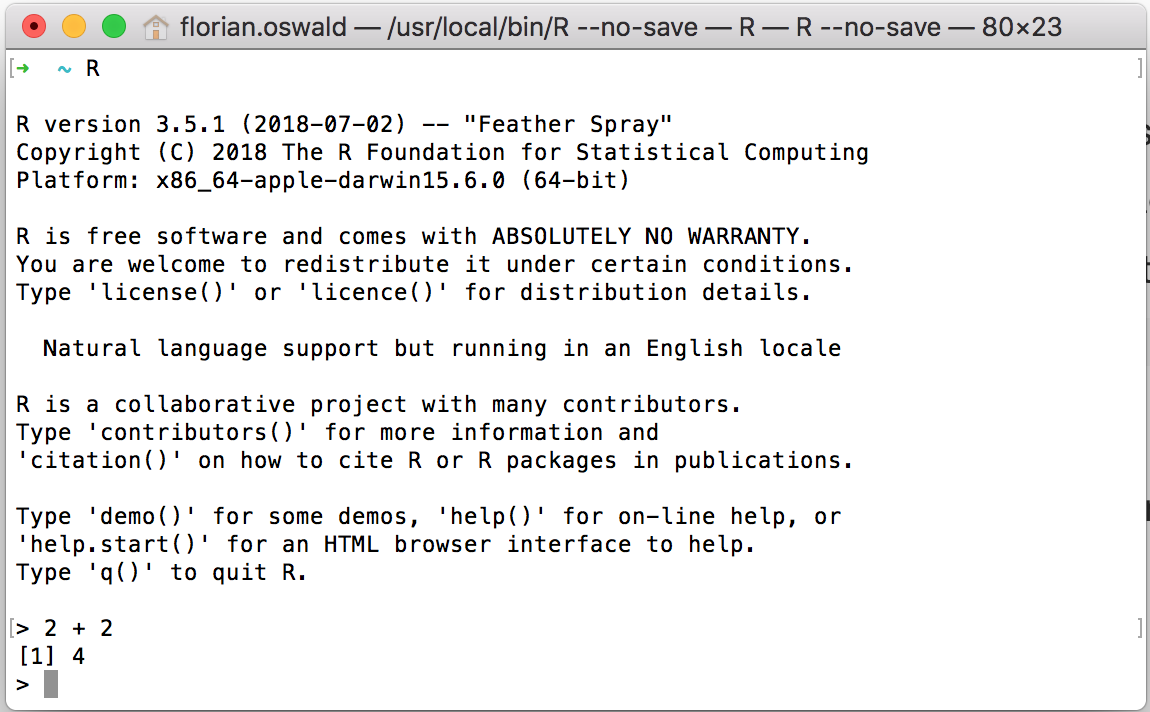
\includegraphics[width=0.5\linewidth]{images/console} 

}

\caption{R GUI symbol and R in a MacOS Terminal}\label{fig:console2}
\end{figure}

Typing one command after the other into the console is not very
convenient as our analysis becomes more involved. Ideally, we would like
to collect all command statements in a file and run them one after the
other, automatically. We can do this by writing so-called \textbf{script
files} or just \textbf{scripts}, i.e.~simple text files with extension
\texttt{.R} or \texttt{.r} which can be \emph{inserted} (or
\emph{sourced}) into an \texttt{R} session. RStudio makes this process
very easy.

Open \texttt{RStudio} by clicking on the \texttt{RStudio} application on
your computer, and notice how different the whole environment is from
the basic \texttt{R} console -- in fact, that \emph{very same}
\texttt{R} console is running in your bottom left panel. The upper-left
panel is a space for you to write scripts -- that is to say many lines
of codes which you can run when you choose to. To run a single line of
code, simply highlight it and hit \texttt{Command} + \texttt{Return}.

\begin{note}
We highly recommend that you use \texttt{RStudio} for everything related
to this course (in particular, to launch our apps and tutorials).
\end{note}

RStudio has a large number of useful keyboard shortcuts. A list of these
can be found using a keyboard shortcut -- the keyboard shortcut to rule
them all:

\begin{itemize}
\tightlist
\item
  On Windows: \texttt{Alt} + \texttt{Shift} + \texttt{K}
\item
  On Mac: \texttt{Option} + \texttt{Shift} + \texttt{K}
\end{itemize}

The \texttt{RStudio} team has developed
\href{https://www.rstudio.com/resources/cheatsheets/}{a number of
``cheatsheets''} for working with both \texttt{R} and \texttt{RStudio}.
\href{http://www.rstudio.com/wp-content/uploads/2016/05/base-r.pdf}{This
particular cheatseet for Base \texttt{R}} will summarize many of the
concepts in this document. \footnote{When programming, it is often a
  good practice to follow a style guide. (Where do spaces go? Tabs or
  spaces? Underscores or CamelCase when naming variables?) No style
  guide is ``correct'' but it helps to be aware of what others do. The
  more import thing is to be consistent within your own code. Here are
  two guides: \href{http://adv-r.had.co.nz/Style.html}{Hadley Wickham
  Style Guide}, and the
  \href{https://google.github.io/styleguide/Rguide.xml}{Google Style
  Guide}. For this course, our main deviation from these two guides is
  the use of \texttt{=} in place of \texttt{\textless{}-}. For all
  practical purposes, you should think \texttt{=} whenever you see
  \texttt{\textless{}-}.}

\subsection{First Glossary}\label{first-glossary}

\begin{itemize}
\tightlist
\item
  \texttt{R}: a statistical programming language
\item
  \texttt{RStudio}: an integrated development environment (IDE) to work
  with \texttt{R}
\item
  \emph{command}: user input (text or numbers) that \texttt{R}
  \emph{understands}.
\item
  \emph{script}: a list of commands collected in a text file, each
  separated by a new line, to be run one after the other.
\end{itemize}

\section{Basic Calculations}\label{basic-calculations}

To get started, we'll use \texttt{R} like a simple calculator. Run the
following code either directly from your RStudio console, or in RStudio
by writting them in a script and running them using \texttt{Command} +
\texttt{Return}.

\subsubsection*{Addition, Subtraction, Multiplication and
Division}\label{addition-subtraction-multiplication-and-division}
\addcontentsline{toc}{subsubsection}{Addition, Subtraction,
Multiplication and Division}

\begin{longtable}[]{@{}ccc@{}}
\toprule
Math & \texttt{R} code & Result\tabularnewline
\midrule
\endhead
\(3 + 2\) & \texttt{3\ +\ 2} & 5\tabularnewline
\(3 - 2\) & \texttt{3\ -\ 2} & 1\tabularnewline
\(3 \cdot2\) & \texttt{3\ *\ 2} & 6\tabularnewline
\(3 / 2\) & \texttt{3\ /\ 2} & 1.5\tabularnewline
\bottomrule
\end{longtable}

\subsubsection*{Exponents}\label{exponents}
\addcontentsline{toc}{subsubsection}{Exponents}

\begin{longtable}[]{@{}ccc@{}}
\toprule
Math & \texttt{R} code & Result\tabularnewline
\midrule
\endhead
\(3^2\) & \texttt{3\ \^{}\ 2} & 9\tabularnewline
\(2^{(-3)}\) & \texttt{2\ \^{}\ (-3)} & 0.125\tabularnewline
\(100^{1/2}\) & \texttt{100\ \^{}\ (1\ /\ 2)} & 10\tabularnewline
\(\sqrt{100}\) & \texttt{sqrt(100)} & 10\tabularnewline
\bottomrule
\end{longtable}

\subsubsection*{Mathematical Constants}\label{mathematical-constants}
\addcontentsline{toc}{subsubsection}{Mathematical Constants}

\begin{longtable}[]{@{}ccc@{}}
\toprule
Math & \texttt{R} code & Result\tabularnewline
\midrule
\endhead
\(\pi\) & \texttt{pi} & 3.1415927\tabularnewline
\(e\) & \texttt{exp(1)} & 2.7182818\tabularnewline
\bottomrule
\end{longtable}

\subsubsection*{Logarithms}\label{logarithms}
\addcontentsline{toc}{subsubsection}{Logarithms}

Note that we will use \(\ln\) and \(\log\) interchangeably to mean the
natural logarithm. There is no \texttt{ln()} in \texttt{R}, instead it
uses \texttt{log()} to mean the natural logarithm.

\begin{longtable}[]{@{}ccc@{}}
\toprule
Math & \texttt{R} code & Result\tabularnewline
\midrule
\endhead
\(\log(e)\) & \texttt{log(exp(1))} & 1\tabularnewline
\(\log_{10}(1000)\) & \texttt{log10(1000)} & 3\tabularnewline
\(\log_{2}(8)\) & \texttt{log2(8)} & 3\tabularnewline
\(\log_{4}(16)\) & \texttt{log(16,\ base\ =\ 4)} & 2\tabularnewline
\bottomrule
\end{longtable}

\subsubsection*{Trigonometry}\label{trigonometry}
\addcontentsline{toc}{subsubsection}{Trigonometry}

\begin{longtable}[]{@{}ccc@{}}
\toprule
Math & \texttt{R} code & Result\tabularnewline
\midrule
\endhead
\(\sin(\pi / 2)\) & \texttt{sin(pi\ /\ 2)} & 1\tabularnewline
\(\cos(0)\) & \texttt{cos(0)} & 1\tabularnewline
\bottomrule
\end{longtable}

\section{Getting Help}\label{getting-help}

In using \texttt{R} as a calculator, we have seen a number of functions:
\texttt{sqrt()}, \texttt{exp()}, \texttt{log()} and \texttt{sin()}. To
get documentation about a function in \texttt{R}, simply put a question
mark in front of the function name, or call the function
\texttt{help(function)} and RStudio will display the documentation, for
example:

\begin{Shaded}
\begin{Highlighting}[]
\NormalTok{?log}
\NormalTok{?sin}
\NormalTok{?paste}
\NormalTok{?lm}
\KeywordTok{help}\NormalTok{(lm)   }\CommentTok{# help() is equivalent}
\KeywordTok{help}\NormalTok{(ggplot,}\DataTypeTok{package=}\StringTok{"ggplot2"}\NormalTok{)  }\CommentTok{# show help from a certain package}
\end{Highlighting}
\end{Shaded}

Frequently one of the most difficult things to do when learning
\texttt{R} is asking for help. First, you need to decide to ask for
help, then you need to know \emph{how} to ask for help. Your very first
line of defense should be to Google your error message or a short
description of your issue. (The ability to solve problems using this
method is quickly becoming an extremely valuable skill.) If that fails,
and it eventually will, you should ask for help. There are a number of
things you should include when contacting an instructor, or posting to a
help website such as \href{https://stackoverflow.com}{Stack Overflow}.

\begin{itemize}
\tightlist
\item
  Describe what you expect the code to do.
\item
  State the end goal you are trying to achieve. (Sometimes what you
  expect the code to do, is not what you want to actually do.)
\item
  Provide the full text of any errors you have received.
\item
  Provide enough code to recreate the error. Often for the purpose of
  this course, you could simply post your entire \texttt{.R} script or
  \texttt{.Rmd} to \texttt{slack}.
\item
  Sometimes it is also helpful to include a screenshot of your entire
  RStudio window when the error occurs.
\end{itemize}

If you follow these steps, you will get your issue resolved much
quicker, and possibly learn more in the process. Do not be discouraged
by running into errors and difficulties when learning \texttt{R}. (Or
any other technical skill.) It is simply part of the learning process.

\section{Installing Packages}\label{installing-packages}

\texttt{R} comes with a number of built-in functions and datasets, but
one of the main strengths of \texttt{R} as an open-source project is its
package system. Packages add additional functions and data. Frequently
if you want to do something in \texttt{R}, and it is not available by
default, there is a good chance that there is a package that will
fulfill your needs.

To install a package, use the \texttt{install.packages()} function.
Think of this as buying a recipe book from the store, bringing it home,
and putting it on your shelf (i.e.~into your library):

\begin{Shaded}
\begin{Highlighting}[]
\KeywordTok{install.packages}\NormalTok{(}\StringTok{"ggplot2"}\NormalTok{)}
\end{Highlighting}
\end{Shaded}

Once a package is installed, it must be loaded into your current
\texttt{R} session before being used. Think of this as taking the book
off of the shelf and opening it up to read.

\begin{Shaded}
\begin{Highlighting}[]
\KeywordTok{library}\NormalTok{(ggplot2)}
\end{Highlighting}
\end{Shaded}

Once you close \texttt{R}, all the packages are closed and put back on
the imaginary shelf. The next time you open \texttt{R}, you do not have
to install the package again, but you do have to load any packages you
intend to use by invoking \texttt{library()}.

\section{\texorpdfstring{\texttt{Code} vs Output in this
Book}{Code vs Output in this Book}}\label{code-output}

A quick note on styling choices in this book. We had to make a decision
how to visually separate \texttt{R} code and resulting output in this
book. We decided to prefix all output lines with
\texttt{\#OUT\textgreater{}} to make the distinction. A typical code
snippet with output is thus going to look like this:

\begin{Shaded}
\begin{Highlighting}[]
\DecValTok{1} \OperatorTok{+}\StringTok{ }\DecValTok{3}
\end{Highlighting}
\end{Shaded}

\begin{verbatim}
#OUT> [1] 4
\end{verbatim}

\begin{Shaded}
\begin{Highlighting}[]
\CommentTok{# everything after a # is a comment, i.e. R disregards it.}
\end{Highlighting}
\end{Shaded}

where you see on the first line the \texttt{R} code, and on the second
line the output. As mentioned, that line starts with
\texttt{\#OUT\textgreater{}} to say \emph{this is an output}, followed
by \texttt{{[}1{]}} (indicating this is a vector of length \emph{one} -
more on this below!), followed by the actual result -
\texttt{1\ +\ 3\ =\ 4}!

Notice that you can simply copy and paste all the code you see into your
\texttt{R} console. In fact, you are \emph{strongly} encouraged to
actually do this and try out \textbf{all the code} you see in this book.

Finally, please note that this way of showing output is fully our choice
in this textbook, and that you should expect other output formats
elsewhere. For example, in my \texttt{RStudio} console, the above code
and output looks like this:

\begin{Shaded}
\begin{Highlighting}[]
\OperatorTok{>}\StringTok{ }\DecValTok{1} \OperatorTok{+}\StringTok{ }\DecValTok{3}
\NormalTok{[}\DecValTok{1}\NormalTok{] }\DecValTok{4}
\end{Highlighting}
\end{Shaded}

\section{\texorpdfstring{\texttt{ScPoEconometrics}
Package}{ScPoEconometrics Package}}\label{install-package}

To fully take advantage of our course, please install the associated
\texttt{R} package directly from its online code repository. You can do
this by copy and pasting the following three lines into your \texttt{R}
console:

\begin{Shaded}
\begin{Highlighting}[]
\ControlFlowTok{if}\NormalTok{ (}\OperatorTok{!}\KeywordTok{require}\NormalTok{(}\StringTok{"devtools"}\NormalTok{)) }\KeywordTok{install.packages}\NormalTok{(}\StringTok{"devtools"}\NormalTok{)}
\KeywordTok{library}\NormalTok{(devtools)}
\KeywordTok{install_github}\NormalTok{(}\DataTypeTok{repo =} \StringTok{"ScPoEcon/ScPoEconometrics"}\NormalTok{)}
\end{Highlighting}
\end{Shaded}

In order to check whether everything works fine, you could load the
library, and check it's current version:

\begin{Shaded}
\begin{Highlighting}[]
\KeywordTok{library}\NormalTok{(ScPoEconometrics)}
\KeywordTok{packageVersion}\NormalTok{(}\StringTok{"ScPoEconometrics"}\NormalTok{)}
\end{Highlighting}
\end{Shaded}

\begin{verbatim}
#OUT> [1] '0.2.0'
\end{verbatim}

\section{Data Types}\label{data-types}

\texttt{R} has a number of basic \emph{data types}. While \texttt{R} is
not a \emph{strongly typed language} (i.e.~you can be agnostic about
types most of the times), it is useful to know what data types are
available to you:

\begin{itemize}
\tightlist
\item
  Numeric

  \begin{itemize}
  \tightlist
  \item
    Also known as Double. The default type when dealing with numbers.
  \item
    Examples: \texttt{1}, \texttt{1.0}, \texttt{42.5}
  \end{itemize}
\item
  Integer

  \begin{itemize}
  \tightlist
  \item
    Examples: \texttt{1L}, \texttt{2L}, \texttt{42L}
  \end{itemize}
\item
  Complex

  \begin{itemize}
  \tightlist
  \item
    Example: \texttt{4\ +\ 2i}
  \end{itemize}
\item
  Logical

  \begin{itemize}
  \tightlist
  \item
    Two possible values: \texttt{TRUE} and \texttt{FALSE}
  \item
    You can also use \texttt{T} and \texttt{F}, but this is \emph{not}
    recommended.
  \item
    \texttt{NA} is also considered logical.
  \end{itemize}
\item
  Character

  \begin{itemize}
  \tightlist
  \item
    Examples: \texttt{"a"}, \texttt{"Statistics"},
    \texttt{"1\ plus\ 2."}
  \end{itemize}
\item
  Categorical or \texttt{factor}

  \begin{itemize}
  \tightlist
  \item
    A mixture of integer and character. A \texttt{factor} variable
    assigns a label to a numeric value.
  \item
    For example \texttt{factor(x=c(0,1),labels=c("male","female"))}
    assigns the string \emph{male} to the numeric values \texttt{0}, and
    the string \emph{female} to the value \texttt{1}.
  \end{itemize}
\end{itemize}

\section{Data Structures}\label{data-structures}

\texttt{R} also has a number of basic data \emph{structures}. A data
structure is either homogeneous (all elements are of the same data type)
or heterogeneous (elements can be of more than one data type).

\begin{longtable}[]{@{}ccc@{}}
\toprule
Dimension & \textbf{Homogeneous} & \textbf{Heterogeneous}\tabularnewline
\midrule
\endhead
1 & Vector & List\tabularnewline
2 & Matrix & Data Frame\tabularnewline
3+ & Array & nested Lists\tabularnewline
\bottomrule
\end{longtable}

\subsection{Vectors}\label{vectors}

Many operations in \texttt{R} make heavy use of \textbf{vectors}. A
vector is a \emph{container} for objects of identical type (see
\ref{data-types} above). Vectors in \texttt{R} are indexed starting at
\texttt{1}. That is what the \texttt{{[}1{]}} in the output is
indicating, that the first element of the row being displayed is the
first element of the vector. Larger vectors will start additional rows
with something like \texttt{{[}7{]}} where \texttt{7} is the index of
the first element of that row.

Possibly the most common way to create a vector in \texttt{R} is using
the \texttt{c()} function, which is short for ``combine''. As the name
suggests, it combines a list of elements separated by commas. (Are you
busy typing all of those examples into your \texttt{R} console? :-) )

\begin{Shaded}
\begin{Highlighting}[]
\KeywordTok{c}\NormalTok{(}\DecValTok{1}\NormalTok{, }\DecValTok{3}\NormalTok{, }\DecValTok{5}\NormalTok{, }\DecValTok{7}\NormalTok{, }\DecValTok{8}\NormalTok{, }\DecValTok{9}\NormalTok{)}
\end{Highlighting}
\end{Shaded}

\begin{verbatim}
#OUT> [1] 1 3 5 7 8 9
\end{verbatim}

Here \texttt{R} simply outputs this vector. If we would like to store
this vector in a \textbf{variable} we can do so with the
\textbf{assignment} operator \texttt{=}. In this case the variable
\texttt{x} now holds the vector we just created, and we can access the
vector by typing \texttt{x}.

\begin{Shaded}
\begin{Highlighting}[]
\NormalTok{x =}\StringTok{ }\KeywordTok{c}\NormalTok{(}\DecValTok{1}\NormalTok{, }\DecValTok{3}\NormalTok{, }\DecValTok{5}\NormalTok{, }\DecValTok{7}\NormalTok{, }\DecValTok{8}\NormalTok{, }\DecValTok{9}\NormalTok{)}
\NormalTok{x}
\end{Highlighting}
\end{Shaded}

\begin{verbatim}
#OUT> [1] 1 3 5 7 8 9
\end{verbatim}

As an aside, there is a long history of the assignment operator in
\texttt{R}, partially due to the keys available on the
\href{https://twitter.com/kwbroman/status/747829864091127809}{keyboards
of the creators of the \texttt{S} language.} (Which preceded
\texttt{R}.) For simplicity we will use \texttt{=}, but know that often
you will see \texttt{\textless{}-} as the assignment operator.

Because vectors must contain elements that are all the same type,
\texttt{R} will automatically \textbf{coerce} (i.e.~convert) to a single
type when attempting to create a vector that combines multiple types.

\begin{Shaded}
\begin{Highlighting}[]
\KeywordTok{c}\NormalTok{(}\DecValTok{42}\NormalTok{, }\StringTok{"Statistics"}\NormalTok{, }\OtherTok{TRUE}\NormalTok{)}
\end{Highlighting}
\end{Shaded}

\begin{verbatim}
#OUT> [1] "42"         "Statistics" "TRUE"
\end{verbatim}

\begin{Shaded}
\begin{Highlighting}[]
\KeywordTok{c}\NormalTok{(}\DecValTok{42}\NormalTok{, }\OtherTok{TRUE}\NormalTok{)}
\end{Highlighting}
\end{Shaded}

\begin{verbatim}
#OUT> [1] 42  1
\end{verbatim}

Frequently you may wish to create a vector based on a sequence of
numbers. The quickest and easiest way to do this is with the \texttt{:}
operator, which creates a sequence of integers between two specified
integers.

\begin{Shaded}
\begin{Highlighting}[]
\NormalTok{(}\DataTypeTok{y =} \DecValTok{1}\OperatorTok{:}\DecValTok{100}\NormalTok{)}
\end{Highlighting}
\end{Shaded}

\begin{verbatim}
#OUT>   [1]   1   2   3   4   5   6   7   8   9  10  11  12  13  14  15  16  17
#OUT>  [18]  18  19  20  21  22  23  24  25  26  27  28  29  30  31  32  33  34
#OUT>  [35]  35  36  37  38  39  40  41  42  43  44  45  46  47  48  49  50  51
#OUT>  [52]  52  53  54  55  56  57  58  59  60  61  62  63  64  65  66  67  68
#OUT>  [69]  69  70  71  72  73  74  75  76  77  78  79  80  81  82  83  84  85
#OUT>  [86]  86  87  88  89  90  91  92  93  94  95  96  97  98  99 100
\end{verbatim}

Here we see \texttt{R} labeling the rows after the first since this is a
large vector. Also, we see that by putting parentheses around the
assignment, \texttt{R} both stores the vector in a variable called
\texttt{y} and automatically outputs \texttt{y} to the console.

Note that scalars do not exists in \texttt{R}. They are simply vectors
of length \texttt{1}.

\begin{Shaded}
\begin{Highlighting}[]
\DecValTok{2}
\end{Highlighting}
\end{Shaded}

\begin{verbatim}
#OUT> [1] 2
\end{verbatim}

If we want to create a sequence that isn't limited to integers and
increasing by 1 at a time, we can use the \texttt{seq()} function.

\begin{Shaded}
\begin{Highlighting}[]
\KeywordTok{seq}\NormalTok{(}\DataTypeTok{from =} \FloatTok{1.5}\NormalTok{, }\DataTypeTok{to =} \FloatTok{4.2}\NormalTok{, }\DataTypeTok{by =} \FloatTok{0.1}\NormalTok{)}
\end{Highlighting}
\end{Shaded}

\begin{verbatim}
#OUT>  [1] 1.5 1.6 1.7 1.8 1.9 2.0 2.1 2.2 2.3 2.4 2.5 2.6 2.7 2.8 2.9 3.0 3.1
#OUT> [18] 3.2 3.3 3.4 3.5 3.6 3.7 3.8 3.9 4.0 4.1 4.2
\end{verbatim}

We will discuss functions in detail later, but note here that the input
labels \texttt{from}, \texttt{to}, and \texttt{by} are optional.

\begin{Shaded}
\begin{Highlighting}[]
\KeywordTok{seq}\NormalTok{(}\FloatTok{1.5}\NormalTok{, }\FloatTok{4.2}\NormalTok{, }\FloatTok{0.1}\NormalTok{)}
\end{Highlighting}
\end{Shaded}

\begin{verbatim}
#OUT>  [1] 1.5 1.6 1.7 1.8 1.9 2.0 2.1 2.2 2.3 2.4 2.5 2.6 2.7 2.8 2.9 3.0 3.1
#OUT> [18] 3.2 3.3 3.4 3.5 3.6 3.7 3.8 3.9 4.0 4.1 4.2
\end{verbatim}

Another common operation to create a vector is \texttt{rep()}, which can
repeat a single value a number of times.

\begin{Shaded}
\begin{Highlighting}[]
\KeywordTok{rep}\NormalTok{(}\StringTok{"A"}\NormalTok{, }\DataTypeTok{times =} \DecValTok{10}\NormalTok{)}
\end{Highlighting}
\end{Shaded}

\begin{verbatim}
#OUT>  [1] "A" "A" "A" "A" "A" "A" "A" "A" "A" "A"
\end{verbatim}

The \texttt{rep()} function can be used to repeat a vector some number
of times.

\begin{Shaded}
\begin{Highlighting}[]
\KeywordTok{rep}\NormalTok{(x, }\DataTypeTok{times =} \DecValTok{3}\NormalTok{)}
\end{Highlighting}
\end{Shaded}

\begin{verbatim}
#OUT>  [1] 1 3 5 7 8 9 1 3 5 7 8 9 1 3 5 7 8 9
\end{verbatim}

We have now seen four different ways to create vectors:

\begin{itemize}
\tightlist
\item
  \texttt{c()}
\item
  \texttt{:}
\item
  \texttt{seq()}
\item
  \texttt{rep()}
\end{itemize}

So far we have mostly used them in isolation, but they are often used
together.

\begin{Shaded}
\begin{Highlighting}[]
\KeywordTok{c}\NormalTok{(x, }\KeywordTok{rep}\NormalTok{(}\KeywordTok{seq}\NormalTok{(}\DecValTok{1}\NormalTok{, }\DecValTok{9}\NormalTok{, }\DecValTok{2}\NormalTok{), }\DecValTok{3}\NormalTok{), }\KeywordTok{c}\NormalTok{(}\DecValTok{1}\NormalTok{, }\DecValTok{2}\NormalTok{, }\DecValTok{3}\NormalTok{), }\DecValTok{42}\NormalTok{, }\DecValTok{2}\OperatorTok{:}\DecValTok{4}\NormalTok{)}
\end{Highlighting}
\end{Shaded}

\begin{verbatim}
#OUT>  [1]  1  3  5  7  8  9  1  3  5  7  9  1  3  5  7  9  1  3  5  7  9  1  2
#OUT> [24]  3 42  2  3  4
\end{verbatim}

The length of a vector can be obtained with the \texttt{length()}
function.

\begin{Shaded}
\begin{Highlighting}[]
\KeywordTok{length}\NormalTok{(x)}
\end{Highlighting}
\end{Shaded}

\begin{verbatim}
#OUT> [1] 6
\end{verbatim}

\begin{Shaded}
\begin{Highlighting}[]
\KeywordTok{length}\NormalTok{(y)}
\end{Highlighting}
\end{Shaded}

\begin{verbatim}
#OUT> [1] 100
\end{verbatim}

\begin{warning}
Let's try this out! \textbf{Your turn}:
\end{warning}

\subsubsection{Task 1}\label{task-1}

\begin{enumerate}
\def\labelenumi{\arabic{enumi}.}
\tightlist
\item
  Create a vector of five ones, i.e. \texttt{{[}1,1,1,1,1{]}}
\item
  Notice that the colon operator \texttt{a:b} is just short for
  \emph{construct a sequence \textbf{from} \texttt{a} \textbf{to}
  \texttt{b}}. Create a vector the counts down from 10 to 0, i.e.~it
  looks like \texttt{{[}10,9,8,7,6,5,4,3,2,1,0{]}}!
\item
  the \texttt{rep} function takes additional arguments \texttt{times}
  (as above), and \texttt{each}, which tells you how often \emph{each
  element} should be repeated (as opposed to the entire input vector).
  Use \texttt{rep} to create a vector that looks like this:
  \texttt{{[}1\ 1\ 1\ 2\ 2\ 2\ 3\ 3\ 3\ 1\ 1\ 1\ 2\ 2\ 2\ 3\ 3\ 3{]}}
\end{enumerate}

\subsubsection{Subsetting}\label{subsetting}

To subset a vector, i.e.~to choose only some elements of it, we use
square brackets, \texttt{{[}{]}}. Here we see that \texttt{x{[}1{]}}
returns the first element, and \texttt{x{[}3{]}} returns the third
element:

\begin{Shaded}
\begin{Highlighting}[]
\NormalTok{x}
\end{Highlighting}
\end{Shaded}

\begin{verbatim}
#OUT> [1] 1 3 5 7 8 9
\end{verbatim}

\begin{Shaded}
\begin{Highlighting}[]
\NormalTok{x[}\DecValTok{1}\NormalTok{]}
\end{Highlighting}
\end{Shaded}

\begin{verbatim}
#OUT> [1] 1
\end{verbatim}

\begin{Shaded}
\begin{Highlighting}[]
\NormalTok{x[}\DecValTok{3}\NormalTok{]}
\end{Highlighting}
\end{Shaded}

\begin{verbatim}
#OUT> [1] 5
\end{verbatim}

We can also exclude certain indexes, in this case the second element.

\begin{Shaded}
\begin{Highlighting}[]
\NormalTok{x[}\OperatorTok{-}\DecValTok{2}\NormalTok{]}
\end{Highlighting}
\end{Shaded}

\begin{verbatim}
#OUT> [1] 1 5 7 8 9
\end{verbatim}

Lastly we see that we can subset based on a vector of indices.

\begin{Shaded}
\begin{Highlighting}[]
\NormalTok{x[}\DecValTok{1}\OperatorTok{:}\DecValTok{3}\NormalTok{]}
\end{Highlighting}
\end{Shaded}

\begin{verbatim}
#OUT> [1] 1 3 5
\end{verbatim}

\begin{Shaded}
\begin{Highlighting}[]
\NormalTok{x[}\KeywordTok{c}\NormalTok{(}\DecValTok{1}\NormalTok{,}\DecValTok{3}\NormalTok{,}\DecValTok{4}\NormalTok{)]}
\end{Highlighting}
\end{Shaded}

\begin{verbatim}
#OUT> [1] 1 5 7
\end{verbatim}

All of the above are subsetting a vector using a vector of indexes.
(Remember a single number is still a vector.) We could instead use a
vector of logical values.

\begin{Shaded}
\begin{Highlighting}[]
\NormalTok{z =}\StringTok{ }\KeywordTok{c}\NormalTok{(}\OtherTok{TRUE}\NormalTok{, }\OtherTok{TRUE}\NormalTok{, }\OtherTok{FALSE}\NormalTok{, }\OtherTok{TRUE}\NormalTok{, }\OtherTok{TRUE}\NormalTok{, }\OtherTok{FALSE}\NormalTok{)}
\NormalTok{z}
\end{Highlighting}
\end{Shaded}

\begin{verbatim}
#OUT> [1]  TRUE  TRUE FALSE  TRUE  TRUE FALSE
\end{verbatim}

\begin{Shaded}
\begin{Highlighting}[]
\NormalTok{x[z]}
\end{Highlighting}
\end{Shaded}

\begin{verbatim}
#OUT> [1] 1 3 7 8
\end{verbatim}

\texttt{R} is able to perform many operations on vectors and scalars
alike:

\begin{Shaded}
\begin{Highlighting}[]
\NormalTok{x =}\StringTok{ }\DecValTok{1}\OperatorTok{:}\DecValTok{10}  \CommentTok{# a vector}
\NormalTok{x }\OperatorTok{+}\StringTok{ }\DecValTok{1}     \CommentTok{# add a scalar}
\end{Highlighting}
\end{Shaded}

\begin{verbatim}
#OUT>  [1]  2  3  4  5  6  7  8  9 10 11
\end{verbatim}

\begin{Shaded}
\begin{Highlighting}[]
\DecValTok{2} \OperatorTok{*}\StringTok{ }\NormalTok{x     }\CommentTok{# multiply all elements by 2}
\end{Highlighting}
\end{Shaded}

\begin{verbatim}
#OUT>  [1]  2  4  6  8 10 12 14 16 18 20
\end{verbatim}

\begin{Shaded}
\begin{Highlighting}[]
\DecValTok{2} \OperatorTok{^}\StringTok{ }\NormalTok{x     }\CommentTok{# take 2 to the x as exponents}
\end{Highlighting}
\end{Shaded}

\begin{verbatim}
#OUT>  [1]    2    4    8   16   32   64  128  256  512 1024
\end{verbatim}

\begin{Shaded}
\begin{Highlighting}[]
\KeywordTok{sqrt}\NormalTok{(x)   }\CommentTok{# compute the square root of all elements in x}
\end{Highlighting}
\end{Shaded}

\begin{verbatim}
#OUT>  [1] 1.000000 1.414214 1.732051 2.000000 2.236068 2.449490 2.645751
#OUT>  [8] 2.828427 3.000000 3.162278
\end{verbatim}

\begin{Shaded}
\begin{Highlighting}[]
\KeywordTok{log}\NormalTok{(x)    }\CommentTok{# take the natural log of all elements in x}
\end{Highlighting}
\end{Shaded}

\begin{verbatim}
#OUT>  [1] 0.0000000 0.6931472 1.0986123 1.3862944 1.6094379 1.7917595 1.9459101
#OUT>  [8] 2.0794415 2.1972246 2.3025851
\end{verbatim}

\begin{Shaded}
\begin{Highlighting}[]
\NormalTok{x }\OperatorTok{+}\StringTok{ }\DecValTok{2}\OperatorTok{*}\NormalTok{x   }\CommentTok{# add vector x to vector 2x}
\end{Highlighting}
\end{Shaded}

\begin{verbatim}
#OUT>  [1]  3  6  9 12 15 18 21 24 27 30
\end{verbatim}

We see that when a function like \texttt{log()} is called on a vector
\texttt{x}, a vector is returned which has applied the function to each
element of the vector \texttt{x}.

\subsection{Logical Operators}\label{logical-operators}

\begin{longtable}[]{@{}lccc@{}}
\toprule
Operator & Summary & Example & Result\tabularnewline
\midrule
\endhead
\texttt{x\ \textless{}\ y} & \texttt{x} less than \texttt{y} &
\texttt{3\ \textless{}\ 42} & TRUE\tabularnewline
\texttt{x\ \textgreater{}\ y} & \texttt{x} greater than \texttt{y} &
\texttt{3\ \textgreater{}\ 42} & FALSE\tabularnewline
\texttt{x\ \textless{}=\ y} & \texttt{x} less than or equal to
\texttt{y} & \texttt{3\ \textless{}=\ 42} & TRUE\tabularnewline
\texttt{x\ \textgreater{}=\ y} & \texttt{x} greater than or equal to
\texttt{y} & \texttt{3\ \textgreater{}=\ 42} & FALSE\tabularnewline
\texttt{x\ ==\ y} & \texttt{x}equal to \texttt{y} & \texttt{3\ ==\ 42} &
FALSE\tabularnewline
\texttt{x\ !=\ y} & \texttt{x} not equal to \texttt{y} &
\texttt{3\ !=\ 42} & TRUE\tabularnewline
\texttt{!x} & not \texttt{x} & \texttt{!(3\ \textgreater{}\ 42)} &
TRUE\tabularnewline
\texttt{x\ \textbar{}\ y} & \texttt{x} or \texttt{y} &
\texttt{(3\ \textgreater{}\ 42)\ \textbar{}\ TRUE} & TRUE\tabularnewline
\texttt{x\ \&\ y} & \texttt{x} and \texttt{y} &
\texttt{(3\ \textless{}\ 4)\ \&\ (\ 42\ \textgreater{}\ 13)} &
TRUE\tabularnewline
\bottomrule
\end{longtable}

In \texttt{R}, logical operators also work on vectors:

\begin{Shaded}
\begin{Highlighting}[]
\NormalTok{x =}\StringTok{ }\KeywordTok{c}\NormalTok{(}\DecValTok{1}\NormalTok{, }\DecValTok{3}\NormalTok{, }\DecValTok{5}\NormalTok{, }\DecValTok{7}\NormalTok{, }\DecValTok{8}\NormalTok{, }\DecValTok{9}\NormalTok{)}
\end{Highlighting}
\end{Shaded}

\begin{Shaded}
\begin{Highlighting}[]
\NormalTok{x }\OperatorTok{>}\StringTok{ }\DecValTok{3}
\end{Highlighting}
\end{Shaded}

\begin{verbatim}
#OUT> [1] FALSE FALSE  TRUE  TRUE  TRUE  TRUE
\end{verbatim}

\begin{Shaded}
\begin{Highlighting}[]
\NormalTok{x }\OperatorTok{<}\StringTok{ }\DecValTok{3}
\end{Highlighting}
\end{Shaded}

\begin{verbatim}
#OUT> [1]  TRUE FALSE FALSE FALSE FALSE FALSE
\end{verbatim}

\begin{Shaded}
\begin{Highlighting}[]
\NormalTok{x }\OperatorTok{==}\StringTok{ }\DecValTok{3}
\end{Highlighting}
\end{Shaded}

\begin{verbatim}
#OUT> [1] FALSE  TRUE FALSE FALSE FALSE FALSE
\end{verbatim}

\begin{Shaded}
\begin{Highlighting}[]
\NormalTok{x }\OperatorTok{!=}\StringTok{ }\DecValTok{3}
\end{Highlighting}
\end{Shaded}

\begin{verbatim}
#OUT> [1]  TRUE FALSE  TRUE  TRUE  TRUE  TRUE
\end{verbatim}

\begin{Shaded}
\begin{Highlighting}[]
\NormalTok{x }\OperatorTok{==}\StringTok{ }\DecValTok{3} \OperatorTok{&}\StringTok{ }\NormalTok{x }\OperatorTok{!=}\StringTok{ }\DecValTok{3}
\end{Highlighting}
\end{Shaded}

\begin{verbatim}
#OUT> [1] FALSE FALSE FALSE FALSE FALSE FALSE
\end{verbatim}

\begin{Shaded}
\begin{Highlighting}[]
\NormalTok{x }\OperatorTok{==}\StringTok{ }\DecValTok{3} \OperatorTok{|}\StringTok{ }\NormalTok{x }\OperatorTok{!=}\StringTok{ }\DecValTok{3}
\end{Highlighting}
\end{Shaded}

\begin{verbatim}
#OUT> [1] TRUE TRUE TRUE TRUE TRUE TRUE
\end{verbatim}

This is quite useful for subsetting.

\begin{Shaded}
\begin{Highlighting}[]
\NormalTok{x[x }\OperatorTok{>}\StringTok{ }\DecValTok{3}\NormalTok{]}
\end{Highlighting}
\end{Shaded}

\begin{verbatim}
#OUT> [1] 5 7 8 9
\end{verbatim}

\begin{Shaded}
\begin{Highlighting}[]
\NormalTok{x[x }\OperatorTok{!=}\StringTok{ }\DecValTok{3}\NormalTok{]}
\end{Highlighting}
\end{Shaded}

\begin{verbatim}
#OUT> [1] 1 5 7 8 9
\end{verbatim}

\begin{Shaded}
\begin{Highlighting}[]
\KeywordTok{sum}\NormalTok{(x }\OperatorTok{>}\StringTok{ }\DecValTok{3}\NormalTok{)}
\end{Highlighting}
\end{Shaded}

\begin{verbatim}
#OUT> [1] 4
\end{verbatim}

\begin{Shaded}
\begin{Highlighting}[]
\KeywordTok{as.numeric}\NormalTok{(x }\OperatorTok{>}\StringTok{ }\DecValTok{3}\NormalTok{)}
\end{Highlighting}
\end{Shaded}

\begin{verbatim}
#OUT> [1] 0 0 1 1 1 1
\end{verbatim}

Here we saw that using the \texttt{sum()} function on a vector of
logical \texttt{TRUE} and \texttt{FALSE} values that is the result of
\texttt{x\ \textgreater{}\ 3} results in a numeric result: you just
\emph{counted} for how many elements of \texttt{x}, the condition
\texttt{\textgreater{}\ 3} is \texttt{TRUE}. During the call to
\texttt{sum()}, \texttt{R} is first automatically coercing the logical
to numeric where \texttt{TRUE} is \texttt{1} and \texttt{FALSE} is
\texttt{0}. This coercion from logical to numeric happens for most
mathematical operations.

\begin{Shaded}
\begin{Highlighting}[]
\CommentTok{# which(condition of x) returns true/false  }
\CommentTok{# each index of x where condition is true}
\KeywordTok{which}\NormalTok{(x }\OperatorTok{>}\StringTok{ }\DecValTok{3}\NormalTok{)}
\end{Highlighting}
\end{Shaded}

\begin{verbatim}
#OUT> [1] 3 4 5 6
\end{verbatim}

\begin{Shaded}
\begin{Highlighting}[]
\NormalTok{x[}\KeywordTok{which}\NormalTok{(x }\OperatorTok{>}\StringTok{ }\DecValTok{3}\NormalTok{)]}
\end{Highlighting}
\end{Shaded}

\begin{verbatim}
#OUT> [1] 5 7 8 9
\end{verbatim}

\begin{Shaded}
\begin{Highlighting}[]
\KeywordTok{max}\NormalTok{(x)}
\end{Highlighting}
\end{Shaded}

\begin{verbatim}
#OUT> [1] 9
\end{verbatim}

\begin{Shaded}
\begin{Highlighting}[]
\KeywordTok{which}\NormalTok{(x }\OperatorTok{==}\StringTok{ }\KeywordTok{max}\NormalTok{(x))}
\end{Highlighting}
\end{Shaded}

\begin{verbatim}
#OUT> [1] 6
\end{verbatim}

\begin{Shaded}
\begin{Highlighting}[]
\KeywordTok{which.max}\NormalTok{(x)}
\end{Highlighting}
\end{Shaded}

\begin{verbatim}
#OUT> [1] 6
\end{verbatim}

\subsubsection{Task 2}\label{task-2}

\begin{enumerate}
\def\labelenumi{\arabic{enumi}.}
\tightlist
\item
  Create a vector filled with 10 numbers drawn from the uniform
  distribution (hint: use function \texttt{runif}) and store them in
  \texttt{x}.
\item
  Using logical subsetting as above, get all the elements of \texttt{x}
  which are larger than 0.5, and store them in \texttt{y}.
\item
  using the function \texttt{which}, store the \emph{indices} of all the
  elements of \texttt{x} which are larger than 0.5 in \texttt{iy}.
\item
  Check that \texttt{y} and \texttt{x{[}iy{]}} are identical.
\end{enumerate}

\subsection{Matrices}\label{matrices}

\texttt{R} can also be used for \textbf{matrix} calculations. Matrices
have rows and columns containing a single data type. In a matrix, the
order of rows and columns is important. (This is not true of \emph{data
frames}, which we will see later.)

Matrices can be created using the \texttt{matrix} function.

\begin{Shaded}
\begin{Highlighting}[]
\NormalTok{x =}\StringTok{ }\DecValTok{1}\OperatorTok{:}\DecValTok{9}
\NormalTok{x}
\end{Highlighting}
\end{Shaded}

\begin{verbatim}
#OUT> [1] 1 2 3 4 5 6 7 8 9
\end{verbatim}

\begin{Shaded}
\begin{Highlighting}[]
\NormalTok{X =}\StringTok{ }\KeywordTok{matrix}\NormalTok{(x, }\DataTypeTok{nrow =} \DecValTok{3}\NormalTok{, }\DataTypeTok{ncol =} \DecValTok{3}\NormalTok{)}
\NormalTok{X}
\end{Highlighting}
\end{Shaded}

\begin{verbatim}
#OUT>      [,1] [,2] [,3]
#OUT> [1,]    1    4    7
#OUT> [2,]    2    5    8
#OUT> [3,]    3    6    9
\end{verbatim}

Notice here that \texttt{R} is case sensitive (\texttt{x} vs
\texttt{X}).

By default the \texttt{matrix} function fills your data into the matrix
column by column. But we can also tell \texttt{R} to fill rows instead:

\begin{Shaded}
\begin{Highlighting}[]
\NormalTok{Y =}\StringTok{ }\KeywordTok{matrix}\NormalTok{(x, }\DataTypeTok{nrow =} \DecValTok{3}\NormalTok{, }\DataTypeTok{ncol =} \DecValTok{3}\NormalTok{, }\DataTypeTok{byrow =} \OtherTok{TRUE}\NormalTok{)}
\NormalTok{Y}
\end{Highlighting}
\end{Shaded}

\begin{verbatim}
#OUT>      [,1] [,2] [,3]
#OUT> [1,]    1    2    3
#OUT> [2,]    4    5    6
#OUT> [3,]    7    8    9
\end{verbatim}

We can also create a matrix of a specified dimension where every element
is the same, in this case \texttt{0}.

\begin{Shaded}
\begin{Highlighting}[]
\NormalTok{Z =}\StringTok{ }\KeywordTok{matrix}\NormalTok{(}\DecValTok{0}\NormalTok{, }\DecValTok{2}\NormalTok{, }\DecValTok{4}\NormalTok{)}
\NormalTok{Z}
\end{Highlighting}
\end{Shaded}

\begin{verbatim}
#OUT>      [,1] [,2] [,3] [,4]
#OUT> [1,]    0    0    0    0
#OUT> [2,]    0    0    0    0
\end{verbatim}

Like vectors, matrices can be subsetted using square brackets,
\texttt{{[}{]}}. However, since matrices are two-dimensional, we need to
specify both a row and a column when subsetting.

\begin{Shaded}
\begin{Highlighting}[]
\NormalTok{X}
\end{Highlighting}
\end{Shaded}

\begin{verbatim}
#OUT>      [,1] [,2] [,3]
#OUT> [1,]    1    4    7
#OUT> [2,]    2    5    8
#OUT> [3,]    3    6    9
\end{verbatim}

\begin{Shaded}
\begin{Highlighting}[]
\NormalTok{X[}\DecValTok{1}\NormalTok{, }\DecValTok{2}\NormalTok{]}
\end{Highlighting}
\end{Shaded}

\begin{verbatim}
#OUT> [1] 4
\end{verbatim}

Here we accessed the element in the first row and the second column. We
could also subset an entire row or column.

\begin{Shaded}
\begin{Highlighting}[]
\NormalTok{X[}\DecValTok{1}\NormalTok{, ]}
\end{Highlighting}
\end{Shaded}

\begin{verbatim}
#OUT> [1] 1 4 7
\end{verbatim}

\begin{Shaded}
\begin{Highlighting}[]
\NormalTok{X[, }\DecValTok{2}\NormalTok{]}
\end{Highlighting}
\end{Shaded}

\begin{verbatim}
#OUT> [1] 4 5 6
\end{verbatim}

We can also use vectors to subset more than one row or column at a time.
Here we subset to the first and third column of the second row:

\begin{Shaded}
\begin{Highlighting}[]
\NormalTok{X[}\DecValTok{2}\NormalTok{, }\KeywordTok{c}\NormalTok{(}\DecValTok{1}\NormalTok{, }\DecValTok{3}\NormalTok{)]}
\end{Highlighting}
\end{Shaded}

\begin{verbatim}
#OUT> [1] 2 8
\end{verbatim}

Matrices can also be created by combining vectors as columns, using
\texttt{cbind}, or combining vectors as rows, using \texttt{rbind}.

\begin{Shaded}
\begin{Highlighting}[]
\NormalTok{x =}\StringTok{ }\DecValTok{1}\OperatorTok{:}\DecValTok{9}
\KeywordTok{rev}\NormalTok{(x)}
\end{Highlighting}
\end{Shaded}

\begin{verbatim}
#OUT> [1] 9 8 7 6 5 4 3 2 1
\end{verbatim}

\begin{Shaded}
\begin{Highlighting}[]
\KeywordTok{rep}\NormalTok{(}\DecValTok{1}\NormalTok{, }\DecValTok{9}\NormalTok{)}
\end{Highlighting}
\end{Shaded}

\begin{verbatim}
#OUT> [1] 1 1 1 1 1 1 1 1 1
\end{verbatim}

\begin{Shaded}
\begin{Highlighting}[]
\KeywordTok{rbind}\NormalTok{(x, }\KeywordTok{rev}\NormalTok{(x), }\KeywordTok{rep}\NormalTok{(}\DecValTok{1}\NormalTok{, }\DecValTok{9}\NormalTok{))}
\end{Highlighting}
\end{Shaded}

\begin{verbatim}
#OUT>   [,1] [,2] [,3] [,4] [,5] [,6] [,7] [,8] [,9]
#OUT> x    1    2    3    4    5    6    7    8    9
#OUT>      9    8    7    6    5    4    3    2    1
#OUT>      1    1    1    1    1    1    1    1    1
\end{verbatim}

\begin{Shaded}
\begin{Highlighting}[]
\KeywordTok{cbind}\NormalTok{(}\DataTypeTok{col_1 =}\NormalTok{ x, }\DataTypeTok{col_2 =} \KeywordTok{rev}\NormalTok{(x), }\DataTypeTok{col_3 =} \KeywordTok{rep}\NormalTok{(}\DecValTok{1}\NormalTok{, }\DecValTok{9}\NormalTok{))}
\end{Highlighting}
\end{Shaded}

\begin{verbatim}
#OUT>       col_1 col_2 col_3
#OUT>  [1,]     1     9     1
#OUT>  [2,]     2     8     1
#OUT>  [3,]     3     7     1
#OUT>  [4,]     4     6     1
#OUT>  [5,]     5     5     1
#OUT>  [6,]     6     4     1
#OUT>  [7,]     7     3     1
#OUT>  [8,]     8     2     1
#OUT>  [9,]     9     1     1
\end{verbatim}

When using \texttt{rbind} and \texttt{cbind} you can specify
``argument'' names that will be used as column names.

\texttt{R} can then be used to perform matrix calculations.

\begin{Shaded}
\begin{Highlighting}[]
\NormalTok{x =}\StringTok{ }\DecValTok{1}\OperatorTok{:}\DecValTok{9}
\NormalTok{y =}\StringTok{ }\DecValTok{9}\OperatorTok{:}\DecValTok{1}
\NormalTok{X =}\StringTok{ }\KeywordTok{matrix}\NormalTok{(x, }\DecValTok{3}\NormalTok{, }\DecValTok{3}\NormalTok{)}
\NormalTok{Y =}\StringTok{ }\KeywordTok{matrix}\NormalTok{(y, }\DecValTok{3}\NormalTok{, }\DecValTok{3}\NormalTok{)}
\NormalTok{X}
\end{Highlighting}
\end{Shaded}

\begin{verbatim}
#OUT>      [,1] [,2] [,3]
#OUT> [1,]    1    4    7
#OUT> [2,]    2    5    8
#OUT> [3,]    3    6    9
\end{verbatim}

\begin{Shaded}
\begin{Highlighting}[]
\NormalTok{Y}
\end{Highlighting}
\end{Shaded}

\begin{verbatim}
#OUT>      [,1] [,2] [,3]
#OUT> [1,]    9    6    3
#OUT> [2,]    8    5    2
#OUT> [3,]    7    4    1
\end{verbatim}

\begin{Shaded}
\begin{Highlighting}[]
\NormalTok{X }\OperatorTok{+}\StringTok{ }\NormalTok{Y}
\end{Highlighting}
\end{Shaded}

\begin{verbatim}
#OUT>      [,1] [,2] [,3]
#OUT> [1,]   10   10   10
#OUT> [2,]   10   10   10
#OUT> [3,]   10   10   10
\end{verbatim}

\begin{Shaded}
\begin{Highlighting}[]
\NormalTok{X }\OperatorTok{-}\StringTok{ }\NormalTok{Y}
\end{Highlighting}
\end{Shaded}

\begin{verbatim}
#OUT>      [,1] [,2] [,3]
#OUT> [1,]   -8   -2    4
#OUT> [2,]   -6    0    6
#OUT> [3,]   -4    2    8
\end{verbatim}

\begin{Shaded}
\begin{Highlighting}[]
\NormalTok{X }\OperatorTok{*}\StringTok{ }\NormalTok{Y}
\end{Highlighting}
\end{Shaded}

\begin{verbatim}
#OUT>      [,1] [,2] [,3]
#OUT> [1,]    9   24   21
#OUT> [2,]   16   25   16
#OUT> [3,]   21   24    9
\end{verbatim}

\begin{Shaded}
\begin{Highlighting}[]
\NormalTok{X }\OperatorTok{/}\StringTok{ }\NormalTok{Y}
\end{Highlighting}
\end{Shaded}

\begin{verbatim}
#OUT>           [,1]      [,2]     [,3]
#OUT> [1,] 0.1111111 0.6666667 2.333333
#OUT> [2,] 0.2500000 1.0000000 4.000000
#OUT> [3,] 0.4285714 1.5000000 9.000000
\end{verbatim}

Note that \texttt{X\ *\ Y} is \textbf{not} matrix multiplication. It is
\emph{element by element} multiplication. (Same for \texttt{X\ /\ Y}).
Matrix multiplication uses \texttt{\%*\%}. Other matrix functions
include \texttt{t()} which gives the transpose of a matrix and
\texttt{solve()} which returns the inverse of a square matrix if it is
invertible.

\begin{Shaded}
\begin{Highlighting}[]
\NormalTok{X }\OperatorTok\StringTok{ }\NormalTok{Y}
\end{Highlighting}
\end{Shaded}

\begin{verbatim}
#OUT>      [,1] [,2] [,3]
#OUT> [1,]   90   54   18
#OUT> [2,]  114   69   24
#OUT> [3,]  138   84   30
\end{verbatim}

\begin{Shaded}
\begin{Highlighting}[]
\KeywordTok{t}\NormalTok{(X)}
\end{Highlighting}
\end{Shaded}

\begin{verbatim}
#OUT>      [,1] [,2] [,3]
#OUT> [1,]    1    2    3
#OUT> [2,]    4    5    6
#OUT> [3,]    7    8    9
\end{verbatim}

\subsection{Arrays}\label{arrays}

A vector is a one-dimensional array. A matrix is a two-dimensional
array. In \texttt{R} you can create arrays of arbitrary dimensionality
\texttt{N}. Here is how:

\begin{Shaded}
\begin{Highlighting}[]
\NormalTok{d =}\StringTok{ }\DecValTok{1}\OperatorTok{:}\DecValTok{16}
\NormalTok{d3 =}\StringTok{ }\KeywordTok{array}\NormalTok{(}\DataTypeTok{data =}\NormalTok{ d,}\DataTypeTok{dim =} \KeywordTok{c}\NormalTok{(}\DecValTok{4}\NormalTok{,}\DecValTok{2}\NormalTok{,}\DecValTok{2}\NormalTok{))}
\NormalTok{d4 =}\StringTok{ }\KeywordTok{array}\NormalTok{(}\DataTypeTok{data =}\NormalTok{ d,}\DataTypeTok{dim =} \KeywordTok{c}\NormalTok{(}\DecValTok{4}\NormalTok{,}\DecValTok{2}\NormalTok{,}\DecValTok{2}\NormalTok{,}\DecValTok{3}\NormalTok{))  }\CommentTok{# will recycle 1:16}
\NormalTok{d3}
\end{Highlighting}
\end{Shaded}

\begin{verbatim}
#OUT> , , 1
#OUT> 
#OUT>      [,1] [,2]
#OUT> [1,]    1    5
#OUT> [2,]    2    6
#OUT> [3,]    3    7
#OUT> [4,]    4    8
#OUT> 
#OUT> , , 2
#OUT> 
#OUT>      [,1] [,2]
#OUT> [1,]    9   13
#OUT> [2,]   10   14
#OUT> [3,]   11   15
#OUT> [4,]   12   16
\end{verbatim}

You can see that \texttt{d3} are simply \emph{two} (4,2) matrices laid
on top of each other, as if there were \emph{two pages}. Similary,
\texttt{d4} would have two pages, and another 3 registers in a fourth
dimension. And so on. You can subset an array like you would a vector or
a matrix, taking care to index each dimension:

\begin{Shaded}
\begin{Highlighting}[]
\NormalTok{d3[ ,}\DecValTok{1}\NormalTok{,}\DecValTok{1}\NormalTok{]  }\CommentTok{# all elements from col 1, page 1}
\end{Highlighting}
\end{Shaded}

\begin{verbatim}
#OUT> [1] 1 2 3 4
\end{verbatim}

\begin{Shaded}
\begin{Highlighting}[]
\NormalTok{d3[}\DecValTok{2}\OperatorTok{:}\DecValTok{3}\NormalTok{, , ]  }\CommentTok{# rows 2:3 from all pages}
\end{Highlighting}
\end{Shaded}

\begin{verbatim}
#OUT> , , 1
#OUT> 
#OUT>      [,1] [,2]
#OUT> [1,]    2    6
#OUT> [2,]    3    7
#OUT> 
#OUT> , , 2
#OUT> 
#OUT>      [,1] [,2]
#OUT> [1,]   10   14
#OUT> [2,]   11   15
\end{verbatim}

\begin{Shaded}
\begin{Highlighting}[]
\NormalTok{d3[}\DecValTok{2}\NormalTok{,}\DecValTok{2}\NormalTok{, ]  }\CommentTok{# row 2, col 2 from both pages.}
\end{Highlighting}
\end{Shaded}

\begin{verbatim}
#OUT> [1]  6 14
\end{verbatim}

\subsubsection{Task 3}\label{task-3}

\begin{enumerate}
\def\labelenumi{\arabic{enumi}.}
\tightlist
\item
  Create a vector containing \texttt{1,2,3,4,5} called v.
\item
  Create a (2,5) matrix \texttt{m} containing the data
  \texttt{1,2,3,4,5,6,7,8,9,10}. The first row should be
  \texttt{1,2,3,4,5}.
\item
  Perform matrix multiplication of \texttt{m} with \texttt{v}. Use the
  command \texttt{\%*\%}. What dimension does the output have?
\item
  Why does \texttt{v\ \%*\%\ m} not work?
\end{enumerate}

\subsection{Lists}\label{lists}

A list is a one-dimensional \emph{heterogeneous} data structure. So it
is indexed like a vector with a single integer value (or with a name),
but each element can contain an element of any type. Lists are similar
to a python or julia \texttt{Dict} object. Many \texttt{R} structures
and outputs are lists themselves. Lists are extremely useful and
versatile objects, so make sure you understand their useage:

\begin{Shaded}
\begin{Highlighting}[]
\CommentTok{# creation without fieldnames}
\KeywordTok{list}\NormalTok{(}\DecValTok{42}\NormalTok{, }\StringTok{"Hello"}\NormalTok{, }\OtherTok{TRUE}\NormalTok{)}
\end{Highlighting}
\end{Shaded}

\begin{verbatim}
#OUT> [[1]]
#OUT> [1] 42
#OUT> 
#OUT> [[2]]
#OUT> [1] "Hello"
#OUT> 
#OUT> [[3]]
#OUT> [1] TRUE
\end{verbatim}

\begin{Shaded}
\begin{Highlighting}[]
\CommentTok{# creation with fieldnames}
\NormalTok{ex_list =}\StringTok{ }\KeywordTok{list}\NormalTok{(}
  \DataTypeTok{a =} \KeywordTok{c}\NormalTok{(}\DecValTok{1}\NormalTok{, }\DecValTok{2}\NormalTok{, }\DecValTok{3}\NormalTok{, }\DecValTok{4}\NormalTok{),}
  \DataTypeTok{b =} \OtherTok{TRUE}\NormalTok{,}
  \DataTypeTok{c =} \StringTok{"Hello!"}\NormalTok{,}
  \DataTypeTok{d =} \ControlFlowTok{function}\NormalTok{(}\DataTypeTok{arg =} \DecValTok{42}\NormalTok{) \{}\KeywordTok{print}\NormalTok{(}\StringTok{"Hello World!"}\NormalTok{)\},}
  \DataTypeTok{e =} \KeywordTok{diag}\NormalTok{(}\DecValTok{5}\NormalTok{)}
\NormalTok{)}
\end{Highlighting}
\end{Shaded}

Lists can be subset using two syntaxes, the \texttt{\$} operator, and
square brackets \texttt{{[}{]}}. The \texttt{\$} operator returns a
named \textbf{element} of a list. The \texttt{{[}{]}} syntax returns a
\textbf{list}, while the \texttt{{[}{[}{]}{]}} returns an
\textbf{element} of a list.

\begin{itemize}
\tightlist
\item
  \texttt{ex\_list{[}1{]}} returns a list contain the first element.
\item
  \texttt{ex\_list{[}{[}1{]}{]}} returns the first element of the list,
  in this case, a vector.
\end{itemize}

\begin{Shaded}
\begin{Highlighting}[]
\CommentTok{# subsetting}
\NormalTok{ex_list}\OperatorTok{$}\NormalTok{e}
\end{Highlighting}
\end{Shaded}

\begin{verbatim}
#OUT>      [,1] [,2] [,3] [,4] [,5]
#OUT> [1,]    1    0    0    0    0
#OUT> [2,]    0    1    0    0    0
#OUT> [3,]    0    0    1    0    0
#OUT> [4,]    0    0    0    1    0
#OUT> [5,]    0    0    0    0    1
\end{verbatim}

\begin{Shaded}
\begin{Highlighting}[]
\NormalTok{ex_list[}\DecValTok{1}\OperatorTok{:}\DecValTok{2}\NormalTok{]}
\end{Highlighting}
\end{Shaded}

\begin{verbatim}
#OUT> $a
#OUT> [1] 1 2 3 4
#OUT> 
#OUT> $b
#OUT> [1] TRUE
\end{verbatim}

\begin{Shaded}
\begin{Highlighting}[]
\NormalTok{ex_list[}\DecValTok{1}\NormalTok{]}
\end{Highlighting}
\end{Shaded}

\begin{verbatim}
#OUT> $a
#OUT> [1] 1 2 3 4
\end{verbatim}

\begin{Shaded}
\begin{Highlighting}[]
\NormalTok{ex_list[[}\DecValTok{1}\NormalTok{]]}
\end{Highlighting}
\end{Shaded}

\begin{verbatim}
#OUT> [1] 1 2 3 4
\end{verbatim}

\begin{Shaded}
\begin{Highlighting}[]
\NormalTok{ex_list[}\KeywordTok{c}\NormalTok{(}\StringTok{"e"}\NormalTok{, }\StringTok{"a"}\NormalTok{)]}
\end{Highlighting}
\end{Shaded}

\begin{verbatim}
#OUT> $e
#OUT>      [,1] [,2] [,3] [,4] [,5]
#OUT> [1,]    1    0    0    0    0
#OUT> [2,]    0    1    0    0    0
#OUT> [3,]    0    0    1    0    0
#OUT> [4,]    0    0    0    1    0
#OUT> [5,]    0    0    0    0    1
#OUT> 
#OUT> $a
#OUT> [1] 1 2 3 4
\end{verbatim}

\begin{Shaded}
\begin{Highlighting}[]
\NormalTok{ex_list[}\StringTok{"e"}\NormalTok{]}
\end{Highlighting}
\end{Shaded}

\begin{verbatim}
#OUT> $e
#OUT>      [,1] [,2] [,3] [,4] [,5]
#OUT> [1,]    1    0    0    0    0
#OUT> [2,]    0    1    0    0    0
#OUT> [3,]    0    0    1    0    0
#OUT> [4,]    0    0    0    1    0
#OUT> [5,]    0    0    0    0    1
\end{verbatim}

\begin{Shaded}
\begin{Highlighting}[]
\NormalTok{ex_list[[}\StringTok{"e"}\NormalTok{]]}
\end{Highlighting}
\end{Shaded}

\begin{verbatim}
#OUT>      [,1] [,2] [,3] [,4] [,5]
#OUT> [1,]    1    0    0    0    0
#OUT> [2,]    0    1    0    0    0
#OUT> [3,]    0    0    1    0    0
#OUT> [4,]    0    0    0    1    0
#OUT> [5,]    0    0    0    0    1
\end{verbatim}

\begin{Shaded}
\begin{Highlighting}[]
\NormalTok{ex_list}\OperatorTok{$}\NormalTok{d}
\end{Highlighting}
\end{Shaded}

\begin{verbatim}
#OUT> function(arg = 42) {print("Hello World!")}
\end{verbatim}

\begin{Shaded}
\begin{Highlighting}[]
\NormalTok{ex_list}\OperatorTok{$}\KeywordTok{d}\NormalTok{(}\DataTypeTok{arg =} \DecValTok{1}\NormalTok{)}
\end{Highlighting}
\end{Shaded}

\begin{verbatim}
#OUT> [1] "Hello World!"
\end{verbatim}

\subsubsection{Task 4}\label{task-4}

\begin{enumerate}
\def\labelenumi{\arabic{enumi}.}
\tightlist
\item
  Copy and paste the above code for \texttt{ex\_list} into your R
  session. Remember that \texttt{list} can hold any kind of \texttt{R}
  object. Like\ldots{}another list! So, create a new list
  \texttt{new\_list} that has two fields: a first field called ``this''
  with string content \texttt{"is\ awesome"}, and a second field called
  ``ex\_list'' that contains \texttt{ex\_list}.
\item
  Accessing members is like in a plain list, just with several layers
  now. Get the element \texttt{c} from \texttt{ex\_list} in
  \texttt{new\_list}!
\item
  Compose a new string out of the first element in \texttt{new\_list},
  the element under label \texttt{this}. Use the function \texttt{paste}
  to print \texttt{R\ is\ awesome} to your screen.
\end{enumerate}

\section{Data Frames}\label{dataframes}

We have previously seen vectors and matrices for storing data as we
introduced \texttt{R}. We will now introduce a \textbf{data frame} which
will be the most common way that we store and interact with data in this
course. A \texttt{data.frame} is similar to a python
\texttt{pandas.dataframe} or a julia \texttt{DataFrame}. (But the
\texttt{R} version was the first! :-) )

\begin{Shaded}
\begin{Highlighting}[]
\NormalTok{example_data =}\StringTok{ }\KeywordTok{data.frame}\NormalTok{(}\DataTypeTok{x =} \KeywordTok{c}\NormalTok{(}\DecValTok{1}\NormalTok{, }\DecValTok{3}\NormalTok{, }\DecValTok{5}\NormalTok{, }\DecValTok{7}\NormalTok{, }\DecValTok{9}\NormalTok{, }\DecValTok{1}\NormalTok{, }\DecValTok{3}\NormalTok{, }\DecValTok{5}\NormalTok{, }\DecValTok{7}\NormalTok{, }\DecValTok{9}\NormalTok{),}
                          \DataTypeTok{y =} \KeywordTok{c}\NormalTok{(}\KeywordTok{rep}\NormalTok{(}\StringTok{"Hello"}\NormalTok{, }\DecValTok{9}\NormalTok{), }\StringTok{"Goodbye"}\NormalTok{),}
                          \DataTypeTok{z =} \KeywordTok{rep}\NormalTok{(}\KeywordTok{c}\NormalTok{(}\OtherTok{TRUE}\NormalTok{, }\OtherTok{FALSE}\NormalTok{), }\DecValTok{5}\NormalTok{))}
\end{Highlighting}
\end{Shaded}

Unlike a matrix, which can be thought of as a vector rearranged into
rows and columns, a data frame is not required to have the same data
type for each element. A data frame is a \textbf{list} of vectors, and
each vector has a \emph{name}. So, each vector must contain the same
data type, but the different vectors can store different data types.
Note, however, that all vectors must have \textbf{the same length}
(differently from a \texttt{list})!

\begin{tip}
A \textbf{data.frame} is similar to a typical Spreadsheet. There are
\emph{rows}, and there are \emph{columns}. A row is typically thought of
as an \emph{observation}, and each column is a certain \emph{variable},
\emph{characteristic} or \emph{feature} of that observation.
\end{tip}

 Let's look at the data frame we just created above:

\begin{Shaded}
\begin{Highlighting}[]
\NormalTok{example_data}
\end{Highlighting}
\end{Shaded}

\begin{verbatim}
#OUT>    x       y     z
#OUT> 1  1   Hello  TRUE
#OUT> 2  3   Hello FALSE
#OUT> 3  5   Hello  TRUE
#OUT> 4  7   Hello FALSE
#OUT> 5  9   Hello  TRUE
#OUT> 6  1   Hello FALSE
#OUT> 7  3   Hello  TRUE
#OUT> 8  5   Hello FALSE
#OUT> 9  7   Hello  TRUE
#OUT> 10 9 Goodbye FALSE
\end{verbatim}

Unlike a list, which has more flexibility, the elements of a data frame
must all be vectors. Again, we access any given column with the
\texttt{\$} operator:

\begin{Shaded}
\begin{Highlighting}[]
\NormalTok{example_data}\OperatorTok{$}\NormalTok{x}
\end{Highlighting}
\end{Shaded}

\begin{verbatim}
#OUT>  [1] 1 3 5 7 9 1 3 5 7 9
\end{verbatim}

\begin{Shaded}
\begin{Highlighting}[]
\KeywordTok{all.equal}\NormalTok{(}\KeywordTok{length}\NormalTok{(example_data}\OperatorTok{$}\NormalTok{x),}
          \KeywordTok{length}\NormalTok{(example_data}\OperatorTok{$}\NormalTok{y),}
          \KeywordTok{length}\NormalTok{(example_data}\OperatorTok{$}\NormalTok{z))}
\end{Highlighting}
\end{Shaded}

\begin{verbatim}
#OUT> [1] TRUE
\end{verbatim}

\begin{Shaded}
\begin{Highlighting}[]
\KeywordTok{str}\NormalTok{(example_data)}
\end{Highlighting}
\end{Shaded}

\begin{verbatim}
#OUT> 'data.frame': 10 obs. of  3 variables:
#OUT>  $ x: num  1 3 5 7 9 1 3 5 7 9
#OUT>  $ y: Factor w/ 2 levels "Goodbye","Hello": 2 2 2 2 2 2 2 2 2 1
#OUT>  $ z: logi  TRUE FALSE TRUE FALSE TRUE FALSE ...
\end{verbatim}

\begin{Shaded}
\begin{Highlighting}[]
\KeywordTok{nrow}\NormalTok{(example_data)}
\end{Highlighting}
\end{Shaded}

\begin{verbatim}
#OUT> [1] 10
\end{verbatim}

\begin{Shaded}
\begin{Highlighting}[]
\KeywordTok{ncol}\NormalTok{(example_data)}
\end{Highlighting}
\end{Shaded}

\begin{verbatim}
#OUT> [1] 3
\end{verbatim}

\begin{Shaded}
\begin{Highlighting}[]
\KeywordTok{dim}\NormalTok{(example_data)}
\end{Highlighting}
\end{Shaded}

\begin{verbatim}
#OUT> [1] 10  3
\end{verbatim}

\begin{Shaded}
\begin{Highlighting}[]
\KeywordTok{names}\NormalTok{(example_data)}
\end{Highlighting}
\end{Shaded}

\begin{verbatim}
#OUT> [1] "x" "y" "z"
\end{verbatim}

\subsection{\texorpdfstring{Working with
\texttt{data.frames}}{Working with data.frames}}\label{working-with-data.frames}

The \texttt{data.frame()} function above is one way to create a data
frame. We can also import data from various file types in into
\texttt{R}, as well as use data stored in packages.

To read this data back into \texttt{R}, we will use the built-in
function \texttt{read.csv}:

\begin{Shaded}
\begin{Highlighting}[]
\NormalTok{path =}\StringTok{ }\KeywordTok{system.file}\NormalTok{(}\DataTypeTok{package=}\StringTok{"ScPoEconometrics"}\NormalTok{,}\StringTok{"datasets"}\NormalTok{,}\StringTok{"example-data.csv"}\NormalTok{)}
\NormalTok{example_data_from_disk =}\StringTok{ }\KeywordTok{read.csv}\NormalTok{(path)}
\end{Highlighting}
\end{Shaded}

This particular line of code assumes that you installed the associated R
package to this book, hence you have this dataset stored on your
computer at
\texttt{system.file(package\ =\ "ScPoEconometrics","datasets","example-data.csv")}.

\begin{Shaded}
\begin{Highlighting}[]
\NormalTok{example_data_from_disk}
\end{Highlighting}
\end{Shaded}

\begin{verbatim}
#OUT>    x       y     z
#OUT> 1  1   Hello  TRUE
#OUT> 2  3   Hello FALSE
#OUT> 3  5   Hello  TRUE
#OUT> 4  7   Hello FALSE
#OUT> 5  9   Hello  TRUE
#OUT> 6  1   Hello FALSE
#OUT> 7  3   Hello  TRUE
#OUT> 8  5   Hello FALSE
#OUT> 9  7   Hello  TRUE
#OUT> 10 9 Goodbye FALSE
\end{verbatim}

When using data, there are three things we would generally like to do:

\begin{itemize}
\tightlist
\item
  Look at the raw data.
\item
  Understand the data. (Where did it come from? What are the variables?
  Etc.)
\item
  Visualize the data.
\end{itemize}

To look at data in a \texttt{data.frame}, we have two useful commands:
\texttt{head()} and \texttt{str()}.

\begin{Shaded}
\begin{Highlighting}[]
\CommentTok{# we are working with the built-in mtcars dataset:}
\NormalTok{mtcars}
\end{Highlighting}
\end{Shaded}

\begin{verbatim}
#OUT>                      mpg cyl  disp  hp drat    wt  qsec vs am gear carb
#OUT> Mazda RX4           21.0   6 160.0 110 3.90 2.620 16.46  0  1    4    4
#OUT> Mazda RX4 Wag       21.0   6 160.0 110 3.90 2.875 17.02  0  1    4    4
#OUT> Datsun 710          22.8   4 108.0  93 3.85 2.320 18.61  1  1    4    1
#OUT> Hornet 4 Drive      21.4   6 258.0 110 3.08 3.215 19.44  1  0    3    1
#OUT> Hornet Sportabout   18.7   8 360.0 175 3.15 3.440 17.02  0  0    3    2
#OUT> Valiant             18.1   6 225.0 105 2.76 3.460 20.22  1  0    3    1
#OUT> Duster 360          14.3   8 360.0 245 3.21 3.570 15.84  0  0    3    4
#OUT> Merc 240D           24.4   4 146.7  62 3.69 3.190 20.00  1  0    4    2
#OUT> Merc 230            22.8   4 140.8  95 3.92 3.150 22.90  1  0    4    2
#OUT> Merc 280            19.2   6 167.6 123 3.92 3.440 18.30  1  0    4    4
#OUT> Merc 280C           17.8   6 167.6 123 3.92 3.440 18.90  1  0    4    4
#OUT> Merc 450SE          16.4   8 275.8 180 3.07 4.070 17.40  0  0    3    3
#OUT> Merc 450SL          17.3   8 275.8 180 3.07 3.730 17.60  0  0    3    3
#OUT> Merc 450SLC         15.2   8 275.8 180 3.07 3.780 18.00  0  0    3    3
#OUT> Cadillac Fleetwood  10.4   8 472.0 205 2.93 5.250 17.98  0  0    3    4
#OUT> Lincoln Continental 10.4   8 460.0 215 3.00 5.424 17.82  0  0    3    4
#OUT> Chrysler Imperial   14.7   8 440.0 230 3.23 5.345 17.42  0  0    3    4
#OUT> Fiat 128            32.4   4  78.7  66 4.08 2.200 19.47  1  1    4    1
#OUT> Honda Civic         30.4   4  75.7  52 4.93 1.615 18.52  1  1    4    2
#OUT> Toyota Corolla      33.9   4  71.1  65 4.22 1.835 19.90  1  1    4    1
#OUT> Toyota Corona       21.5   4 120.1  97 3.70 2.465 20.01  1  0    3    1
#OUT> Dodge Challenger    15.5   8 318.0 150 2.76 3.520 16.87  0  0    3    2
#OUT> AMC Javelin         15.2   8 304.0 150 3.15 3.435 17.30  0  0    3    2
#OUT> Camaro Z28          13.3   8 350.0 245 3.73 3.840 15.41  0  0    3    4
#OUT> Pontiac Firebird    19.2   8 400.0 175 3.08 3.845 17.05  0  0    3    2
#OUT> Fiat X1-9           27.3   4  79.0  66 4.08 1.935 18.90  1  1    4    1
#OUT> Porsche 914-2       26.0   4 120.3  91 4.43 2.140 16.70  0  1    5    2
#OUT> Lotus Europa        30.4   4  95.1 113 3.77 1.513 16.90  1  1    5    2
#OUT> Ford Pantera L      15.8   8 351.0 264 4.22 3.170 14.50  0  1    5    4
#OUT> Ferrari Dino        19.7   6 145.0 175 3.62 2.770 15.50  0  1    5    6
#OUT> Maserati Bora       15.0   8 301.0 335 3.54 3.570 14.60  0  1    5    8
#OUT> Volvo 142E          21.4   4 121.0 109 4.11 2.780 18.60  1  1    4    2
\end{verbatim}

You can see that this prints the entire data.frame to screen. The
function \texttt{head()} will display the first \texttt{n} observations
of the data frame.

\begin{Shaded}
\begin{Highlighting}[]
\KeywordTok{head}\NormalTok{(mtcars,}\DataTypeTok{n=}\DecValTok{2}\NormalTok{)}
\end{Highlighting}
\end{Shaded}

\begin{verbatim}
#OUT>               mpg cyl disp  hp drat    wt  qsec vs am gear carb
#OUT> Mazda RX4      21   6  160 110  3.9 2.620 16.46  0  1    4    4
#OUT> Mazda RX4 Wag  21   6  160 110  3.9 2.875 17.02  0  1    4    4
\end{verbatim}

\begin{Shaded}
\begin{Highlighting}[]
\KeywordTok{head}\NormalTok{(mtcars) }\CommentTok{# default}
\end{Highlighting}
\end{Shaded}

\begin{verbatim}
#OUT>                    mpg cyl disp  hp drat    wt  qsec vs am gear carb
#OUT> Mazda RX4         21.0   6  160 110 3.90 2.620 16.46  0  1    4    4
#OUT> Mazda RX4 Wag     21.0   6  160 110 3.90 2.875 17.02  0  1    4    4
#OUT> Datsun 710        22.8   4  108  93 3.85 2.320 18.61  1  1    4    1
#OUT> Hornet 4 Drive    21.4   6  258 110 3.08 3.215 19.44  1  0    3    1
#OUT> Hornet Sportabout 18.7   8  360 175 3.15 3.440 17.02  0  0    3    2
#OUT> Valiant           18.1   6  225 105 2.76 3.460 20.22  1  0    3    1
\end{verbatim}

The function \texttt{str()} will display the ``structure'' of the data
frame. It will display the number of \textbf{observations} and
\textbf{variables}, list the variables, give the type of each variable,
and show some elements of each variable. This information can also be
found in the ``Environment'' window in RStudio.

\begin{Shaded}
\begin{Highlighting}[]
\KeywordTok{str}\NormalTok{(mtcars)}
\end{Highlighting}
\end{Shaded}

\begin{verbatim}
#OUT> 'data.frame': 32 obs. of  11 variables:
#OUT>  $ mpg : num  21 21 22.8 21.4 18.7 18.1 14.3 24.4 22.8 19.2 ...
#OUT>  $ cyl : num  6 6 4 6 8 6 8 4 4 6 ...
#OUT>  $ disp: num  160 160 108 258 360 ...
#OUT>  $ hp  : num  110 110 93 110 175 105 245 62 95 123 ...
#OUT>  $ drat: num  3.9 3.9 3.85 3.08 3.15 2.76 3.21 3.69 3.92 3.92 ...
#OUT>  $ wt  : num  2.62 2.88 2.32 3.21 3.44 ...
#OUT>  $ qsec: num  16.5 17 18.6 19.4 17 ...
#OUT>  $ vs  : num  0 0 1 1 0 1 0 1 1 1 ...
#OUT>  $ am  : num  1 1 1 0 0 0 0 0 0 0 ...
#OUT>  $ gear: num  4 4 4 3 3 3 3 4 4 4 ...
#OUT>  $ carb: num  4 4 1 1 2 1 4 2 2 4 ...
\end{verbatim}

In this dataset an observation is for a particular model of a car, and
the variables describe attributes of the car, for example its fuel
efficiency, or its weight.

To understand more about the data set, we use the \texttt{?} operator to
pull up the documentation for the data.

\begin{Shaded}
\begin{Highlighting}[]
\NormalTok{?mtcars}
\end{Highlighting}
\end{Shaded}

\texttt{R} has a number of functions for quickly working with and
extracting basic information from data frames. To quickly obtain a
vector of the variable names, we use the \texttt{names()} function.

\begin{Shaded}
\begin{Highlighting}[]
\KeywordTok{names}\NormalTok{(mtcars)}
\end{Highlighting}
\end{Shaded}

\begin{verbatim}
#OUT>  [1] "mpg"  "cyl"  "disp" "hp"   "drat" "wt"   "qsec" "vs"   "am"   "gear"
#OUT> [11] "carb"
\end{verbatim}

To access one of the variables \textbf{as a vector}, we use the
\texttt{\$} operator.

\begin{Shaded}
\begin{Highlighting}[]
\NormalTok{mtcars}\OperatorTok{$}\NormalTok{mpg}
\end{Highlighting}
\end{Shaded}

\begin{verbatim}
#OUT>  [1] 21.0 21.0 22.8 21.4 18.7 18.1 14.3 24.4 22.8 19.2 17.8 16.4 17.3 15.2
#OUT> [15] 10.4 10.4 14.7 32.4 30.4 33.9 21.5 15.5 15.2 13.3 19.2 27.3 26.0 30.4
#OUT> [29] 15.8 19.7 15.0 21.4
\end{verbatim}

\begin{Shaded}
\begin{Highlighting}[]
\NormalTok{mtcars}\OperatorTok{$}\NormalTok{wt}
\end{Highlighting}
\end{Shaded}

\begin{verbatim}
#OUT>  [1] 2.620 2.875 2.320 3.215 3.440 3.460 3.570 3.190 3.150 3.440 3.440
#OUT> [12] 4.070 3.730 3.780 5.250 5.424 5.345 2.200 1.615 1.835 2.465 3.520
#OUT> [23] 3.435 3.840 3.845 1.935 2.140 1.513 3.170 2.770 3.570 2.780
\end{verbatim}

We can use the \texttt{dim()}, \texttt{nrow()} and \texttt{ncol()}
functions to obtain information about the dimension of the data frame.

\begin{Shaded}
\begin{Highlighting}[]
\KeywordTok{dim}\NormalTok{(mtcars)}
\end{Highlighting}
\end{Shaded}

\begin{verbatim}
#OUT> [1] 32 11
\end{verbatim}

\begin{Shaded}
\begin{Highlighting}[]
\KeywordTok{nrow}\NormalTok{(mtcars)}
\end{Highlighting}
\end{Shaded}

\begin{verbatim}
#OUT> [1] 32
\end{verbatim}

\begin{Shaded}
\begin{Highlighting}[]
\KeywordTok{ncol}\NormalTok{(mtcars)}
\end{Highlighting}
\end{Shaded}

\begin{verbatim}
#OUT> [1] 11
\end{verbatim}

Here \texttt{nrow()} is also the number of observations, which in most
cases is the \emph{sample size}.

Subsetting data frames can work much like subsetting matrices using
square brackets, \texttt{{[}\ ,\ {]}}. Here, we find vehicles with mpg
over 25 miles per gallon and only display columns \texttt{cyl},
\texttt{disp} and \texttt{wt}.

\begin{Shaded}
\begin{Highlighting}[]
\CommentTok{# mpg[row condition, col condition]}
\NormalTok{mtcars[mtcars}\OperatorTok{$}\NormalTok{mpg }\OperatorTok{>}\StringTok{ }\DecValTok{20}\NormalTok{, }\KeywordTok{c}\NormalTok{(}\StringTok{"cyl"}\NormalTok{, }\StringTok{"disp"}\NormalTok{, }\StringTok{"wt"}\NormalTok{)]}
\end{Highlighting}
\end{Shaded}

\begin{verbatim}
#OUT>                cyl  disp    wt
#OUT> Mazda RX4        6 160.0 2.620
#OUT> Mazda RX4 Wag    6 160.0 2.875
#OUT> Datsun 710       4 108.0 2.320
#OUT> Hornet 4 Drive   6 258.0 3.215
#OUT> Merc 240D        4 146.7 3.190
#OUT> Merc 230         4 140.8 3.150
#OUT> Fiat 128         4  78.7 2.200
#OUT> Honda Civic      4  75.7 1.615
#OUT> Toyota Corolla   4  71.1 1.835
#OUT> Toyota Corona    4 120.1 2.465
#OUT> Fiat X1-9        4  79.0 1.935
#OUT> Porsche 914-2    4 120.3 2.140
#OUT> Lotus Europa     4  95.1 1.513
#OUT> Volvo 142E       4 121.0 2.780
\end{verbatim}

An alternative would be to use the \texttt{subset()} function, which has
a much more readable syntax.

\begin{Shaded}
\begin{Highlighting}[]
\KeywordTok{subset}\NormalTok{(mtcars, }\DataTypeTok{subset =}\NormalTok{ mpg }\OperatorTok{>}\StringTok{ }\DecValTok{25}\NormalTok{, }\DataTypeTok{select =} \KeywordTok{c}\NormalTok{(}\StringTok{"cyl"}\NormalTok{, }\StringTok{"disp"}\NormalTok{, }\StringTok{"wt"}\NormalTok{))}
\end{Highlighting}
\end{Shaded}

\subsubsection{Task 5}\label{task-5}

\begin{enumerate}
\def\labelenumi{\arabic{enumi}.}
\tightlist
\item
  How many observations are there in \texttt{mtcars}?
\item
  How many variables?
\item
  What is the average value of \texttt{mpg}?
\item
  What is the average value of \texttt{mpg} for cars with more than 4
  cylinders, i.e.~with \texttt{cyl\textgreater{}4}?
\end{enumerate}

\section{Programming Basics}\label{programming-basics}

In this section we illustrate some general concepts related to
programming.

\subsection{Variables}\label{variables}

We encountered the term \emph{variable} already several times, but
mainly in the context of a column of a data.frame. In programming, a
variable is denotes an \emph{object}. Another way to say it is that a
variable is a name or a \emph{label} for something:

\begin{Shaded}
\begin{Highlighting}[]
\NormalTok{x =}\StringTok{ }\DecValTok{1}
\NormalTok{y =}\StringTok{ "roses"}
\NormalTok{z =}\StringTok{ }\ControlFlowTok{function}\NormalTok{(x)\{}\KeywordTok{sqrt}\NormalTok{(x)\}}
\end{Highlighting}
\end{Shaded}

Here \texttt{x} refers to the value \texttt{1}, \texttt{y} holds the
string ``roses'', and \texttt{z} is the name of a function that computes
\(\sqrt{x}\). Notice that the argument \texttt{x} of the function is
different from the \texttt{x} we just defined. It is \textbf{local} to
the function:

\begin{Shaded}
\begin{Highlighting}[]
\NormalTok{x}
\end{Highlighting}
\end{Shaded}

\begin{verbatim}
#OUT> [1] 1
\end{verbatim}

\begin{Shaded}
\begin{Highlighting}[]
\KeywordTok{z}\NormalTok{(}\DecValTok{9}\NormalTok{)}
\end{Highlighting}
\end{Shaded}

\begin{verbatim}
#OUT> [1] 3
\end{verbatim}

\subsection{Control Flow}\label{control-flow}

Control Flow relates to ways in which you can adapt your code to
different circumstances. Based on a \texttt{condition} being
\texttt{TRUE}, your program will do one thing, as opposed to another
thing. This is most widely known as an \texttt{if/else} statement. In
\texttt{R}, the if/else syntax is:

\begin{Shaded}
\begin{Highlighting}[]
\ControlFlowTok{if}\NormalTok{ (}\DataTypeTok{condition =} \OtherTok{TRUE}\NormalTok{) \{}
\NormalTok{  some R code}
\NormalTok{\} }\ControlFlowTok{else}\NormalTok{ \{}
\NormalTok{  some other R code}
\NormalTok{\}}
\end{Highlighting}
\end{Shaded}

For example,

\begin{Shaded}
\begin{Highlighting}[]
\NormalTok{x =}\StringTok{ }\DecValTok{1}
\NormalTok{y =}\StringTok{ }\DecValTok{3}
\ControlFlowTok{if}\NormalTok{ (x }\OperatorTok{>}\StringTok{ }\NormalTok{y) \{  }\CommentTok{# test if x > y}
  \CommentTok{# if TRUE}
\NormalTok{  z =}\StringTok{ }\NormalTok{x }\OperatorTok{*}\StringTok{ }\NormalTok{y}
  \KeywordTok{print}\NormalTok{(}\StringTok{"x is larger than y"}\NormalTok{)}
\NormalTok{\} }\ControlFlowTok{else}\NormalTok{ \{}
  \CommentTok{# if FALSE}
\NormalTok{  z =}\StringTok{ }\NormalTok{x }\OperatorTok{+}\StringTok{ }\DecValTok{5} \OperatorTok{*}\StringTok{ }\NormalTok{y}
  \KeywordTok{print}\NormalTok{(}\StringTok{"x is less than or equal to y"}\NormalTok{)}
\NormalTok{\}}
\end{Highlighting}
\end{Shaded}

\begin{verbatim}
#OUT> [1] "x is less than or equal to y"
\end{verbatim}

\begin{Shaded}
\begin{Highlighting}[]
\NormalTok{z}
\end{Highlighting}
\end{Shaded}

\begin{verbatim}
#OUT> [1] 16
\end{verbatim}

\subsection{Loops}\label{loops}

Loops are a very important programming construct. As the name suggests,
in a \emph{loop}, the programming \emph{repeatedly} loops over a set of
instructions, until some condition tells it to stop. A very powerful,
yet simple, construction is that the program can \emph{count how many
steps} it has done already - which may be important to know for many
algorithms. The syntax of a \texttt{for} loop (there are others), is

\begin{Shaded}
\begin{Highlighting}[]
\ControlFlowTok{for}\NormalTok{ (ix }\ControlFlowTok{in} \DecValTok{1}\OperatorTok{:}\DecValTok{10}\NormalTok{)\{   }\CommentTok{# does not have to be 1:10!}
  \CommentTok{# loop body: gets executed each time}
  \CommentTok{# the value of ix changes with each iteration}
\NormalTok{\}}
\end{Highlighting}
\end{Shaded}

For example, consider this simple \texttt{for} loop, which will simply
print the value of the \emph{iterator} (called \texttt{i} in this case)
to screen:

\begin{Shaded}
\begin{Highlighting}[]
\ControlFlowTok{for}\NormalTok{ (i }\ControlFlowTok{in} \DecValTok{1}\OperatorTok{:}\DecValTok{5}\NormalTok{)\{}
  \KeywordTok{print}\NormalTok{(i)}
\NormalTok{\}}
\end{Highlighting}
\end{Shaded}

\begin{verbatim}
#OUT> [1] 1
#OUT> [1] 2
#OUT> [1] 3
#OUT> [1] 4
#OUT> [1] 5
\end{verbatim}

Notice that instead of \texttt{1:5}, we could have \emph{any} kind of
iterable collection:

\begin{Shaded}
\begin{Highlighting}[]
\ControlFlowTok{for}\NormalTok{ (i }\ControlFlowTok{in} \KeywordTok{c}\NormalTok{(}\StringTok{"mangos"}\NormalTok{,}\StringTok{"bananas"}\NormalTok{,}\StringTok{"apples"}\NormalTok{))\{}
  \KeywordTok{print}\NormalTok{(}\KeywordTok{paste}\NormalTok{(}\StringTok{"I love"}\NormalTok{,i))  }\CommentTok{# the paste function pastes together strings}
\NormalTok{\}}
\end{Highlighting}
\end{Shaded}

\begin{verbatim}
#OUT> [1] "I love mangos"
#OUT> [1] "I love bananas"
#OUT> [1] "I love apples"
\end{verbatim}

We often also see \emph{nested} loops, which are just what its name
suggests:

\begin{Shaded}
\begin{Highlighting}[]
\ControlFlowTok{for}\NormalTok{ (i }\ControlFlowTok{in} \DecValTok{2}\OperatorTok{:}\DecValTok{3}\NormalTok{)\{}
  \CommentTok{# first nest: for each i}
  \ControlFlowTok{for}\NormalTok{ (j }\ControlFlowTok{in} \KeywordTok{c}\NormalTok{(}\StringTok{"mangos"}\NormalTok{,}\StringTok{"bananas"}\NormalTok{,}\StringTok{"apples"}\NormalTok{))\{}
    \CommentTok{# second nest: for each j}
    \KeywordTok{print}\NormalTok{(}\KeywordTok{paste}\NormalTok{(}\StringTok{"Can I get"}\NormalTok{,i,j,}\StringTok{"please?"}\NormalTok{))}
\NormalTok{  \}}
\NormalTok{\}}
\end{Highlighting}
\end{Shaded}

\begin{verbatim}
#OUT> [1] "Can I get 2 mangos please?"
#OUT> [1] "Can I get 2 bananas please?"
#OUT> [1] "Can I get 2 apples please?"
#OUT> [1] "Can I get 3 mangos please?"
#OUT> [1] "Can I get 3 bananas please?"
#OUT> [1] "Can I get 3 apples please?"
\end{verbatim}

The important thing to note here is that you can do calculations with
the iterators \emph{while inside a loop}.

\subsection{Functions}\label{functions}

So far we have been using functions, but haven't actually discussed some
of their details. A function is a set of instructions that \texttt{R}
executes for us, much like those collected in a script file. The good
thing is that functions are much more flexible than scripts, since they
can depend on \emph{input arguments}, which change the way the function
behaves. Here is how to define a function:

\begin{Shaded}
\begin{Highlighting}[]
\NormalTok{function_name <-}\StringTok{ }\ControlFlowTok{function}\NormalTok{(arg1,}\DataTypeTok{arg2=}\NormalTok{default_value)\{}
  \CommentTok{# function body}
  \CommentTok{# you do stuff with arg1 and arg2}
  \CommentTok{# you can have any number of arguments, with or without defaults}
  \CommentTok{# any valid `R` commands can be included here}
  \CommentTok{# the last line is returned}
\NormalTok{\}}
\end{Highlighting}
\end{Shaded}

And here is a trivial example of a function definition:

\begin{Shaded}
\begin{Highlighting}[]
\NormalTok{hello <-}\StringTok{ }\ControlFlowTok{function}\NormalTok{(}\DataTypeTok{your_name =} \StringTok{"Lord Vader"}\NormalTok{)\{}
  \KeywordTok{paste}\NormalTok{(}\StringTok{"You R most welcome,"}\NormalTok{,your_name)}
  \CommentTok{# we could also write:}
  \CommentTok{# return(paste("You R most welcome,",your_name))}
\NormalTok{\}}

\CommentTok{# we call the function by typing it's name with round brackets}
\KeywordTok{hello}\NormalTok{()}
\end{Highlighting}
\end{Shaded}

\begin{verbatim}
#OUT> [1] "You R most welcome, Lord Vader"
\end{verbatim}

You see that by not specifying the argument \texttt{your\_name},
\texttt{R} reverts to the default value given. Try with your own name
now!

Just typing the function name returns the actual definition to us, which
is handy sometimes:

\begin{Shaded}
\begin{Highlighting}[]
\NormalTok{hello}
\end{Highlighting}
\end{Shaded}

\begin{verbatim}
#OUT> function(your_name = "Lord Vader"){
#OUT>   paste("You R most welcome,",your_name)
#OUT>   # we could also write:
#OUT>   # return(paste("You R most welcome,",your_name))
#OUT> }
\end{verbatim}

It's instructive to consider that before we defined the function
\texttt{hello} above, \texttt{R} did not know what to do, had you called
\texttt{hello()}. The function did not exist! In this sense, we
\emph{taught \texttt{R} a new trick}. This feature to create new
capabilities on top of a core language is one of the most powerful
characteristics of programming languages. In general, it is good
practice to split your code into several smaller functions, rather than
one long script file. It makes your code more readable, and it is easier
to track down mistakes.

\subsubsection{Task 6}\label{task-6}

\begin{enumerate}
\def\labelenumi{\arabic{enumi}.}
\tightlist
\item
  Write a for loop that counts down from 10 to 1, printing the value of
  the iterator to the screen.
\item
  Modify that loop to write ``i iterations to go'' where \texttt{i} is
  the iterator
\item
  Modify that loop so that each iteration takes roughly one second. You
  can achieve that by adding the command \texttt{Sys.sleep(1)} below the
  line that prints ``i iterations to go''.
\end{enumerate}

\chapter{Working With Data}\label{sum}

In this chapter we will first learn some basic concepts that help
summarizing data. Then, we will tackle a real-world task and read,
clean, and summarize data from the web.

\section{Summary Statistics}\label{summary-statistics}

\texttt{R} has built in functions for a large number of summary
statistics. For numeric variables, we can summarize data by looking at
their center and spread, for example.

\begin{Shaded}
\begin{Highlighting}[]
\CommentTok{# for the mpg dataset, we load:}
\KeywordTok{library}\NormalTok{(ggplot2)}
\end{Highlighting}
\end{Shaded}

\subsection*{Central Tendency}\label{central-tendency}
\addcontentsline{toc}{subsection}{Central Tendency}

Suppose we want to know the \emph{mean} and \emph{median} of all the
values stored in the \texttt{data.frame} column \texttt{mpg\$cty}:

\begin{longtable}[]{@{}ccc@{}}
\toprule
Measure & \texttt{R} & Result\tabularnewline
\midrule
\endhead
Mean & \texttt{mean(mpg\$cty)} & 16.8589744\tabularnewline
Median & \texttt{median(mpg\$cty)} & 17\tabularnewline
\bottomrule
\end{longtable}

\subsection*{Spread}\label{spread}
\addcontentsline{toc}{subsection}{Spread}

How do the values in that column \emph{vary}? How far \emph{spread out}
are they?

\begin{longtable}[]{@{}ccc@{}}
\toprule
Measure & \texttt{R} & Result\tabularnewline
\midrule
\endhead
Variance & \texttt{var(mpg\$cty)} & 18.1130736\tabularnewline
Standard Deviation & \texttt{sd(mpg\$cty)} & 4.2559457\tabularnewline
IQR & \texttt{IQR(mpg\$cty)} & 5\tabularnewline
Minimum & \texttt{min(mpg\$cty)} & 9\tabularnewline
Maximum & \texttt{max(mpg\$cty)} & 35\tabularnewline
Range & \texttt{range(mpg\$cty)} & 9, 35\tabularnewline
\bottomrule
\end{longtable}

\subsection*{Categorical}\label{categorical}
\addcontentsline{toc}{subsection}{Categorical}

For categorical variables, counts and percentages can be used for
summary.

\begin{Shaded}
\begin{Highlighting}[]
\KeywordTok{table}\NormalTok{(mpg}\OperatorTok{$}\NormalTok{drv)}
\end{Highlighting}
\end{Shaded}

\begin{verbatim}
#OUT> 
#OUT>   4   f   r 
#OUT> 103 106  25
\end{verbatim}

\begin{Shaded}
\begin{Highlighting}[]
\KeywordTok{table}\NormalTok{(mpg}\OperatorTok{$}\NormalTok{drv) }\OperatorTok{/}\StringTok{ }\KeywordTok{nrow}\NormalTok{(mpg)}
\end{Highlighting}
\end{Shaded}

\begin{verbatim}
#OUT> 
#OUT>         4         f         r 
#OUT> 0.4401709 0.4529915 0.1068376
\end{verbatim}

\section{Plotting}\label{plotting}

Now that we have some data to work with, and we have learned about the
data at the most basic level, our next tasks will be to visualize it.
Often, a proper visualization can illuminate features of the data that
can inform further analysis.

We will look at four methods of visualizing data by using the basic
\texttt{plot} facilities built-in with \texttt{R}:

\begin{itemize}
\tightlist
\item
  Histograms
\item
  Barplots
\item
  Boxplots
\item
  Scatterplots
\end{itemize}

\subsection{Histograms}\label{histograms}

When visualizing a single numerical variable, a \textbf{histogram} is
useful. It summarizes the \emph{distribution} of values in a vector. In
\texttt{R} you create one using the \texttt{hist()} function:

\begin{Shaded}
\begin{Highlighting}[]
\KeywordTok{hist}\NormalTok{(mpg}\OperatorTok{$}\NormalTok{cty)}
\end{Highlighting}
\end{Shaded}

\begin{center}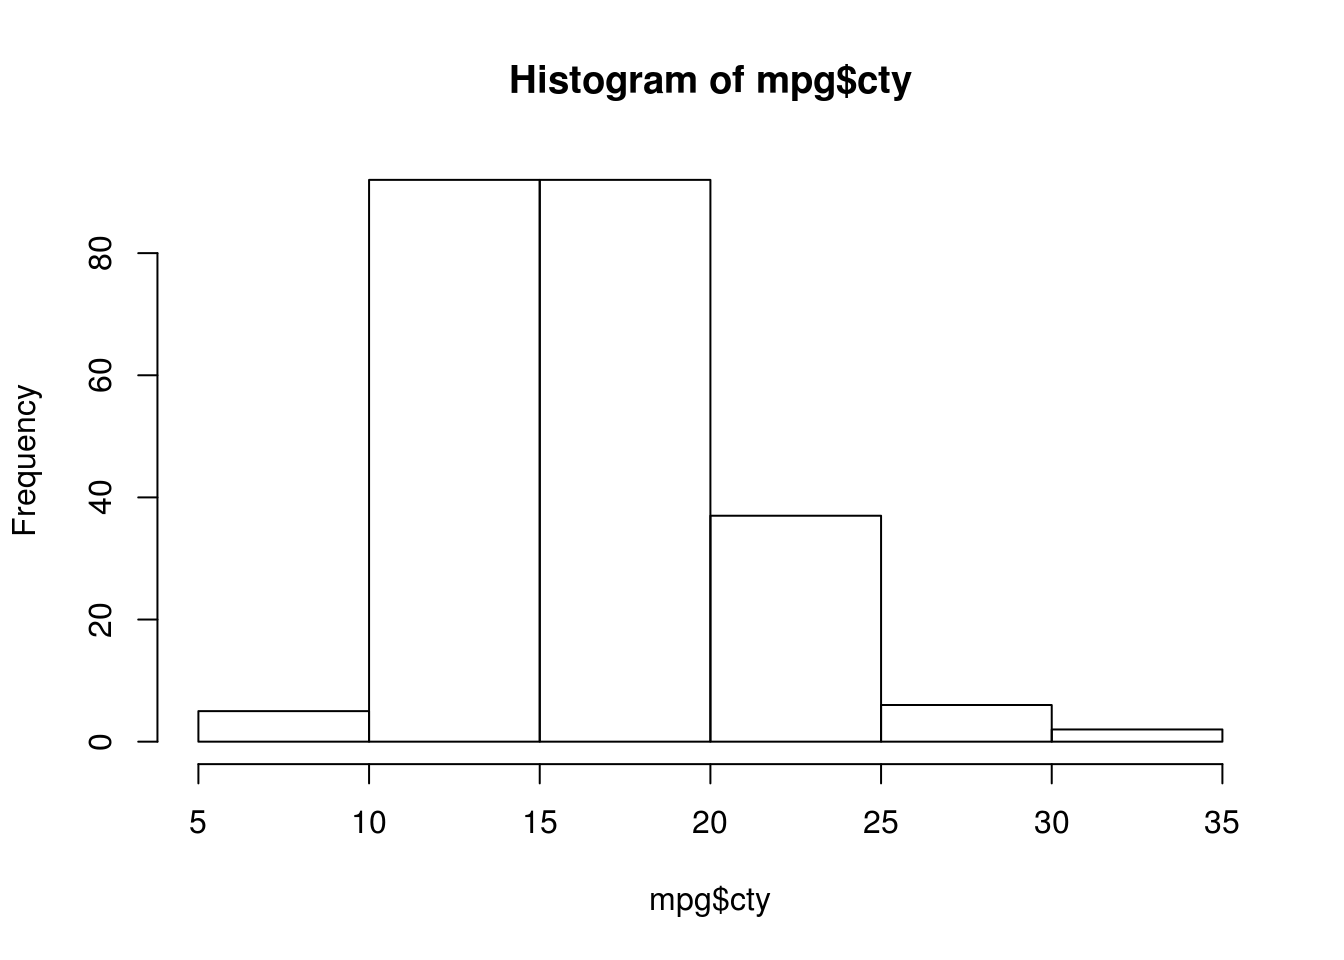
\includegraphics{ScPoEconometrics_files/figure-latex/unnamed-chunk-76-1} \end{center}

The histogram function has a number of parameters which can be changed
to make our plot look much nicer. Use the \texttt{?} operator to read
the documentation for the \texttt{hist()} to see a full list of these
parameters.

\begin{Shaded}
\begin{Highlighting}[]
\KeywordTok{hist}\NormalTok{(mpg}\OperatorTok{$}\NormalTok{cty,}
     \DataTypeTok{xlab   =} \StringTok{"Miles Per Gallon (City)"}\NormalTok{,}
     \DataTypeTok{main   =} \StringTok{"Histogram of MPG (City)"}\NormalTok{, }\CommentTok{# main title}
     \DataTypeTok{breaks =} \DecValTok{12}\NormalTok{,   }\CommentTok{# how many breaks?}
     \DataTypeTok{col    =} \StringTok{"red"}\NormalTok{,}
     \DataTypeTok{border =} \StringTok{"blue"}\NormalTok{)}
\end{Highlighting}
\end{Shaded}

\begin{center}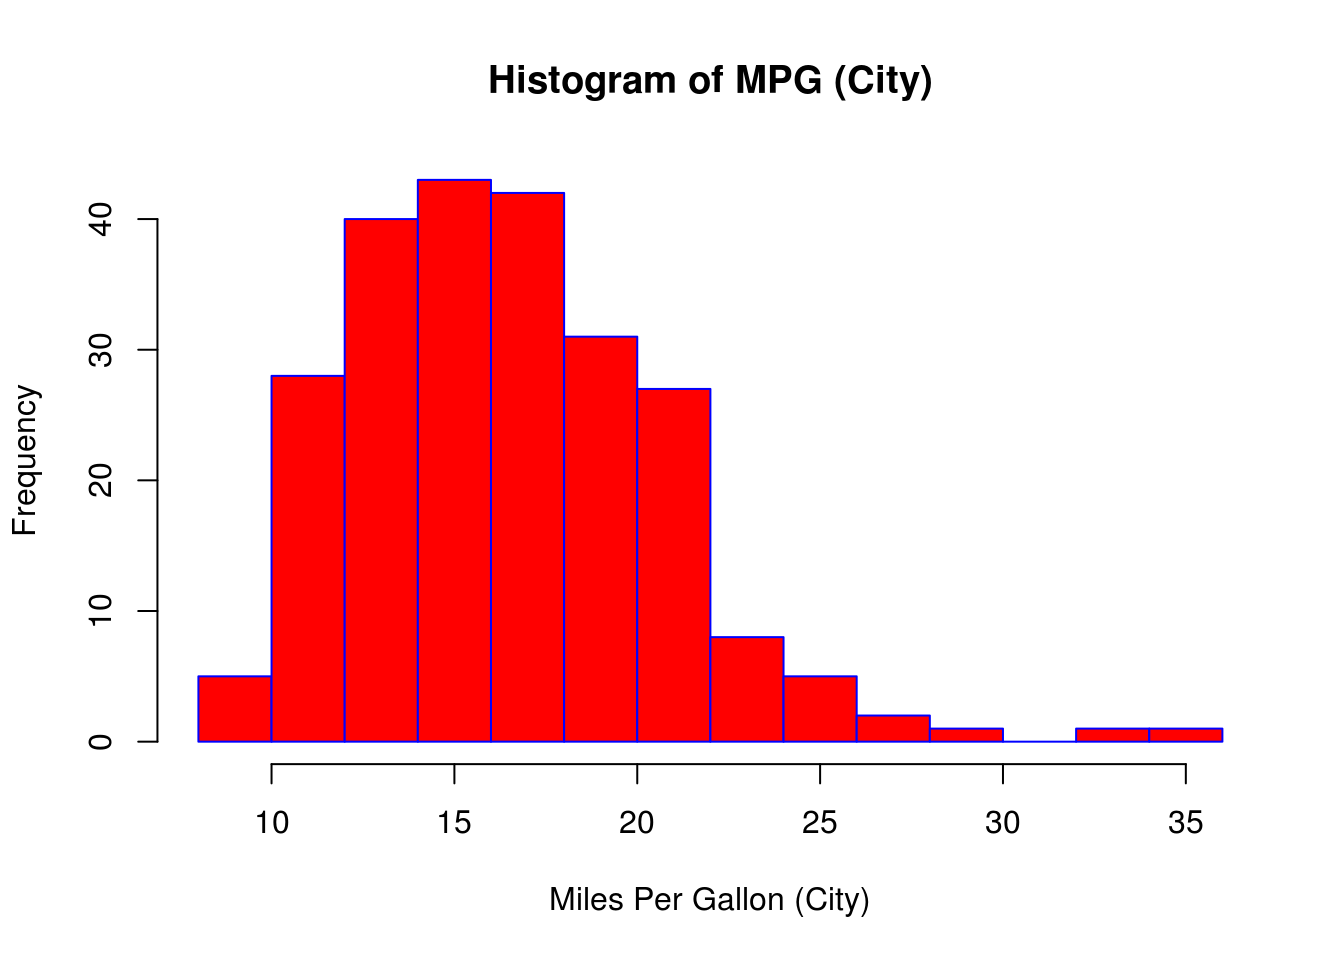
\includegraphics{ScPoEconometrics_files/figure-latex/unnamed-chunk-77-1} \end{center}

Importantly, you should always be sure to label your axes and give the
plot a title. The argument \texttt{breaks} is specific to
\texttt{hist()}. Entering an integer will give a suggestion to
\texttt{R} for how many bars to use for the histogram. By default
\texttt{R} will attempt to intelligently guess a good number of
\texttt{breaks}, but as we can see here, it is sometimes useful to
modify this yourself.

\subsection{Barplots}\label{barplots}

Somewhat similar to a histogram, a barplot can provide a visual summary
of a categorical variable, or a numeric variable with a finite number of
values, like a ranking from 1 to 10.

\begin{Shaded}
\begin{Highlighting}[]
\KeywordTok{barplot}\NormalTok{(}\KeywordTok{table}\NormalTok{(mpg}\OperatorTok{$}\NormalTok{drv))}
\end{Highlighting}
\end{Shaded}

\begin{center}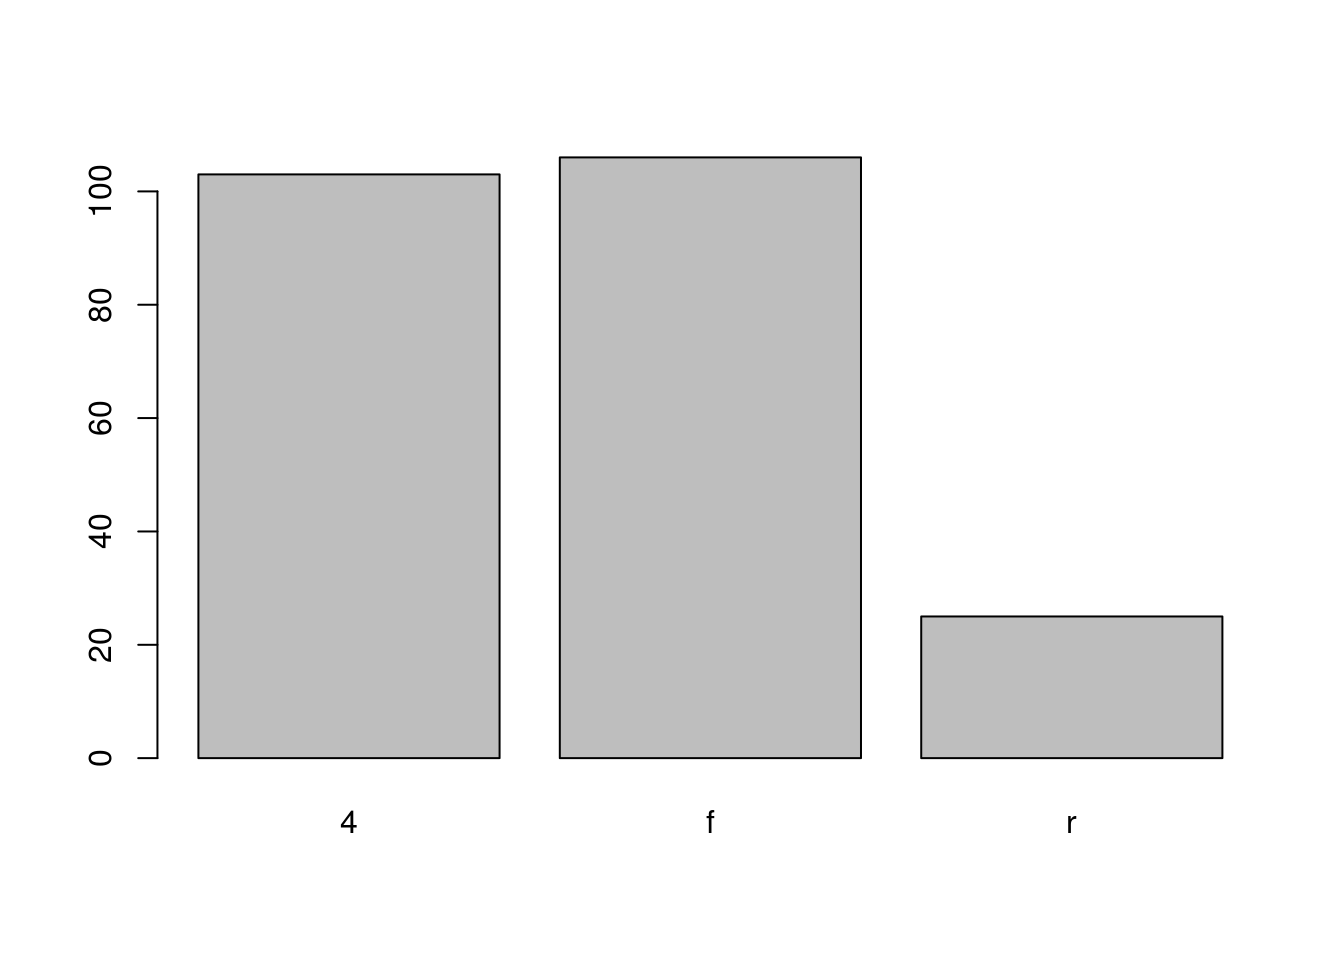
\includegraphics{ScPoEconometrics_files/figure-latex/unnamed-chunk-78-1} \end{center}

\begin{Shaded}
\begin{Highlighting}[]
\KeywordTok{barplot}\NormalTok{(}\KeywordTok{table}\NormalTok{(mpg}\OperatorTok{$}\NormalTok{drv),}
        \DataTypeTok{xlab   =} \StringTok{"Drivetrain (f = FWD, r = RWD, 4 = 4WD)"}\NormalTok{,}
        \DataTypeTok{ylab   =} \StringTok{"Frequency"}\NormalTok{,}
        \DataTypeTok{main   =} \StringTok{"Drivetrains"}\NormalTok{,}
        \DataTypeTok{col    =} \StringTok{"dodgerblue"}\NormalTok{,}
        \DataTypeTok{border =} \StringTok{"darkorange"}\NormalTok{)}
\end{Highlighting}
\end{Shaded}

\begin{center}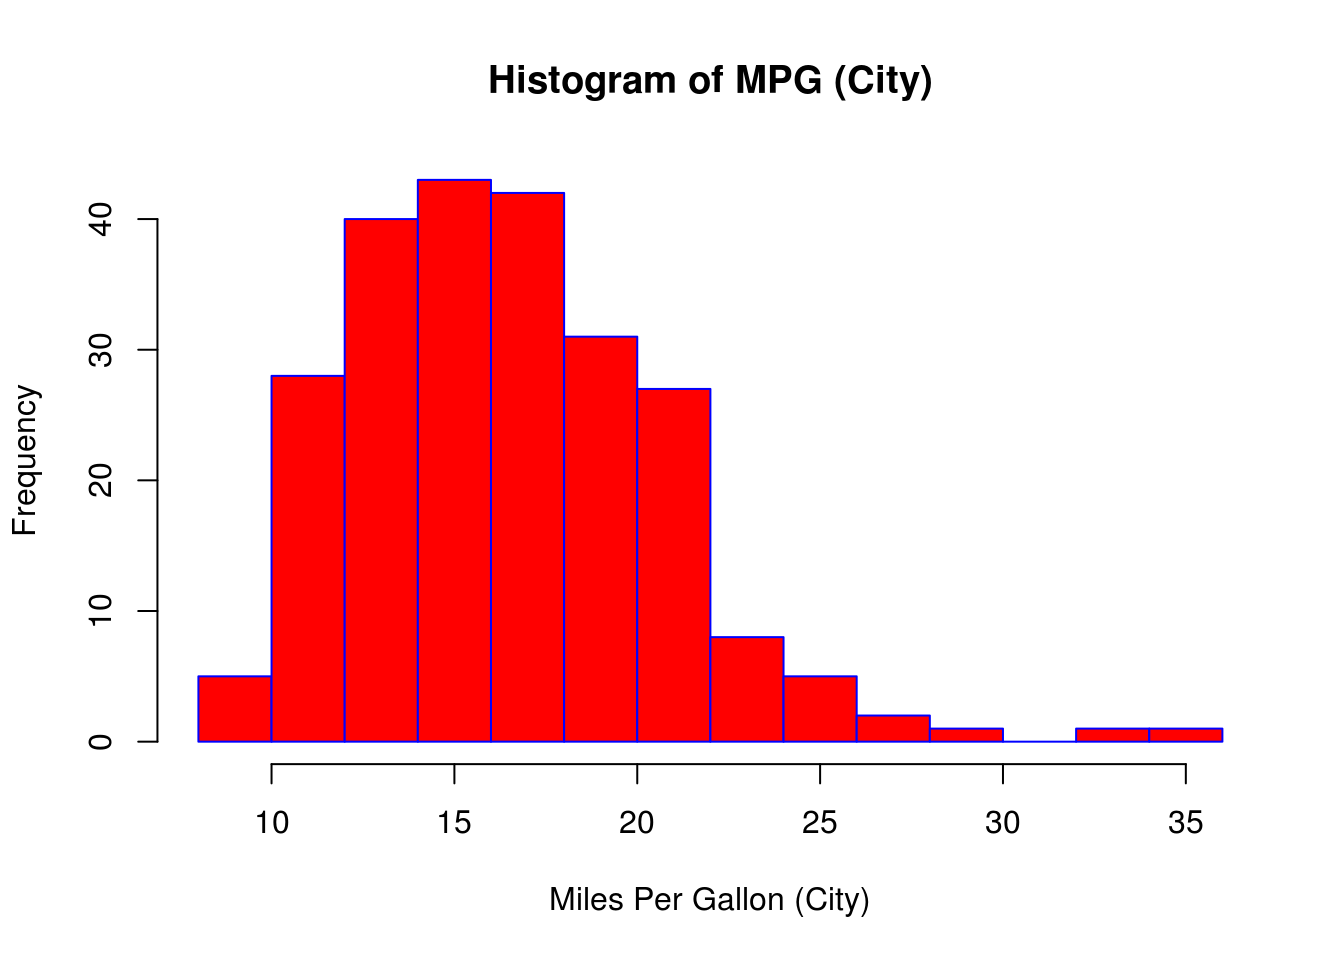
\includegraphics{ScPoEconometrics_files/figure-latex/unnamed-chunk-79-1} \end{center}

\subsection{Boxplots}\label{boxplots}

To visualize the relationship between a numerical and categorical
variable, once could use a \textbf{boxplot}. In the \texttt{mpg}
dataset, the \texttt{drv} variable takes a small, finite number of
values. A car can only be front wheel drive, 4 wheel drive, or rear
wheel drive.

\begin{Shaded}
\begin{Highlighting}[]
\KeywordTok{unique}\NormalTok{(mpg}\OperatorTok{$}\NormalTok{drv)}
\end{Highlighting}
\end{Shaded}

\begin{verbatim}
#OUT> [1] "f" "4" "r"
\end{verbatim}

First note that we can use a single boxplot as an alternative to a
histogram for visualizing a single numerical variable. To do so in
\texttt{R}, we use the \texttt{boxplot()} function. The box shows the
\emph{interquartile range}, the solid line in the middle is the value of
the median, the wiskers show 1.5 times the interquartile range, and the
dots are outliers.

\begin{Shaded}
\begin{Highlighting}[]
\KeywordTok{boxplot}\NormalTok{(mpg}\OperatorTok{$}\NormalTok{hwy)}
\end{Highlighting}
\end{Shaded}

\begin{center}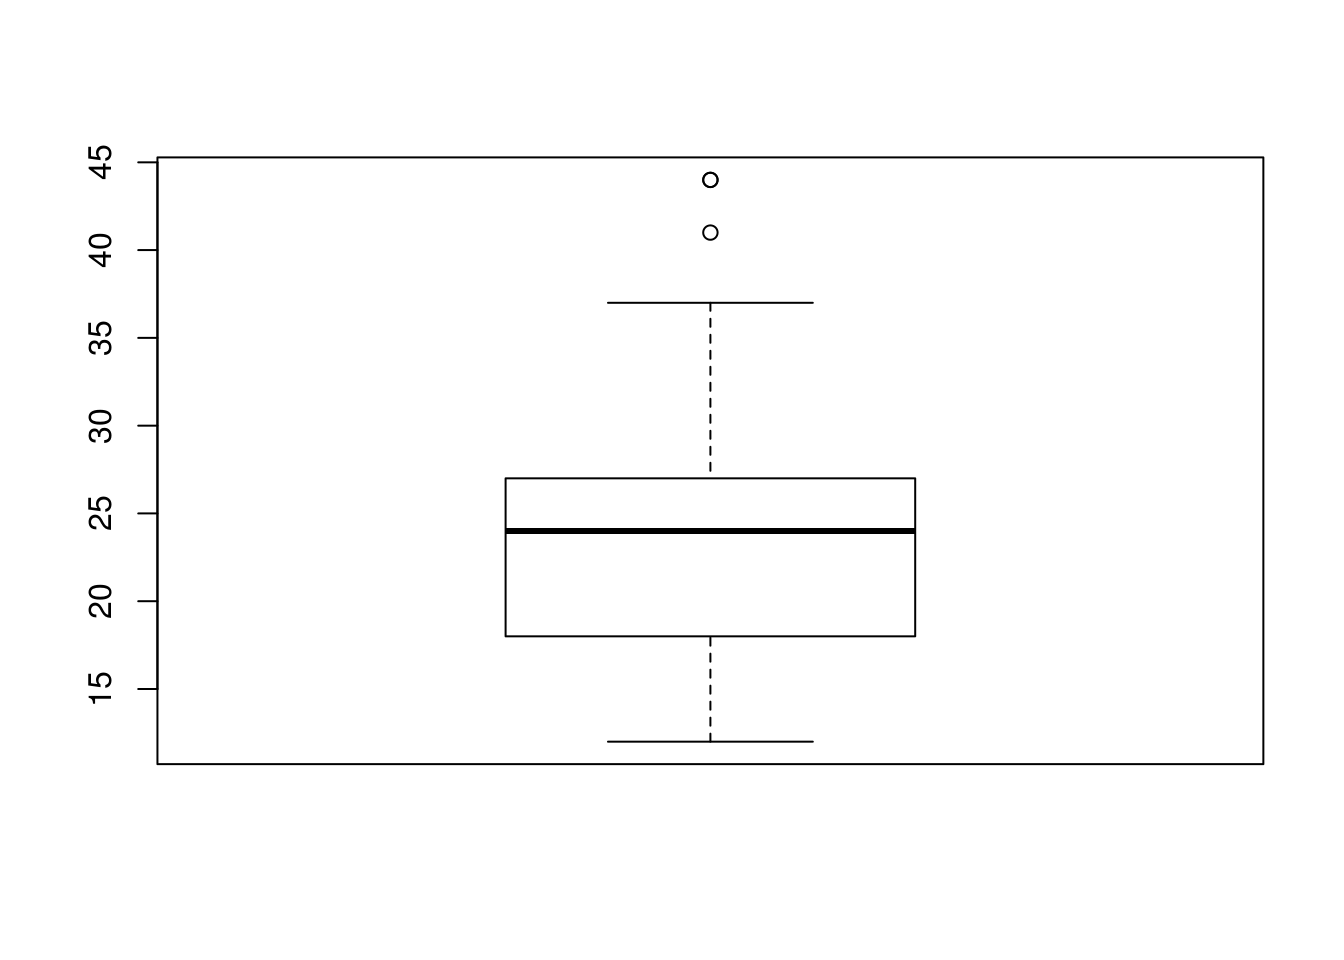
\includegraphics{ScPoEconometrics_files/figure-latex/unnamed-chunk-81-1} \end{center}

However, more often we will use boxplots to compare a numerical variable
for different values of a categorical variable.

\begin{Shaded}
\begin{Highlighting}[]
\KeywordTok{boxplot}\NormalTok{(hwy }\OperatorTok{~}\StringTok{ }\NormalTok{drv, }\DataTypeTok{data =}\NormalTok{ mpg)}
\end{Highlighting}
\end{Shaded}

\begin{center}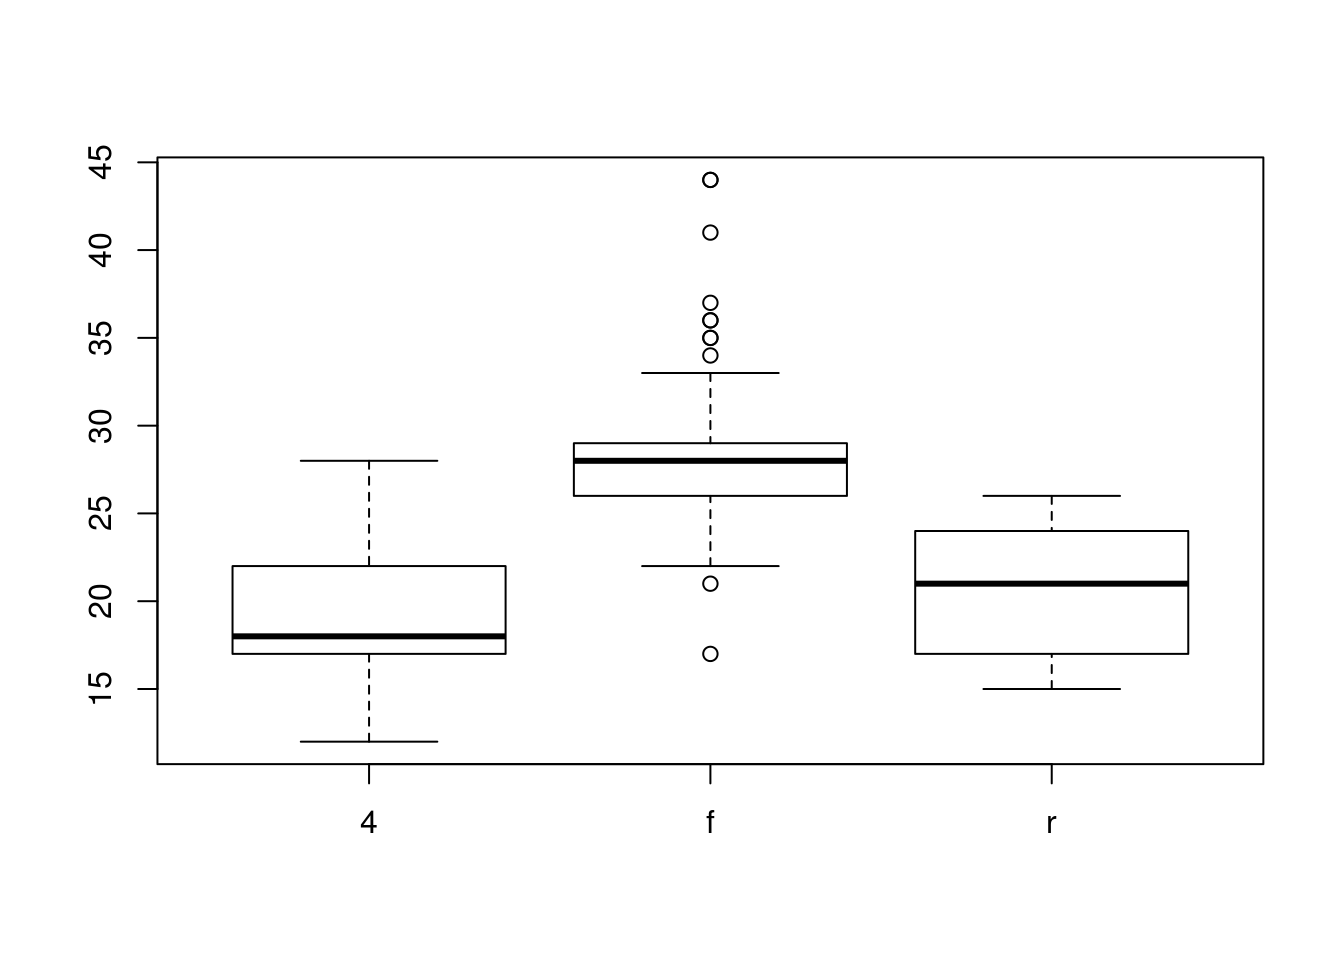
\includegraphics{ScPoEconometrics_files/figure-latex/unnamed-chunk-82-1} \end{center}

Here used the \texttt{boxplot()} command to create side-by-side
boxplots. However, since we are now dealing with two variables, the
syntax has changed. The \texttt{R} syntax
\texttt{hwy\ \textasciitilde{}\ drv,\ data\ =\ mpg} reads ``Plot the
\texttt{hwy} variable against the \texttt{drv} variable using the
dataset \texttt{mpg}.'' We see the use of a \texttt{\textasciitilde{}}
(which specifies a formula) and also a \texttt{data\ =} argument. This
will be a syntax that is common to many functions we will use in this
course.

\begin{Shaded}
\begin{Highlighting}[]
\KeywordTok{boxplot}\NormalTok{(hwy }\OperatorTok{~}\StringTok{ }\NormalTok{drv, }\DataTypeTok{data =}\NormalTok{ mpg,}
     \DataTypeTok{xlab   =} \StringTok{"Drivetrain (f = FWD, r = RWD, 4 = 4WD)"}\NormalTok{,}
     \DataTypeTok{ylab   =} \StringTok{"Miles Per Gallon (Highway)"}\NormalTok{,}
     \DataTypeTok{main   =} \StringTok{"MPG (Highway) vs Drivetrain"}\NormalTok{,}
     \DataTypeTok{pch    =} \DecValTok{20}\NormalTok{,}
     \DataTypeTok{cex    =} \DecValTok{2}\NormalTok{,}
     \DataTypeTok{col    =} \StringTok{"darkorange"}\NormalTok{,}
     \DataTypeTok{border =} \StringTok{"dodgerblue"}\NormalTok{)}
\end{Highlighting}
\end{Shaded}

\begin{center}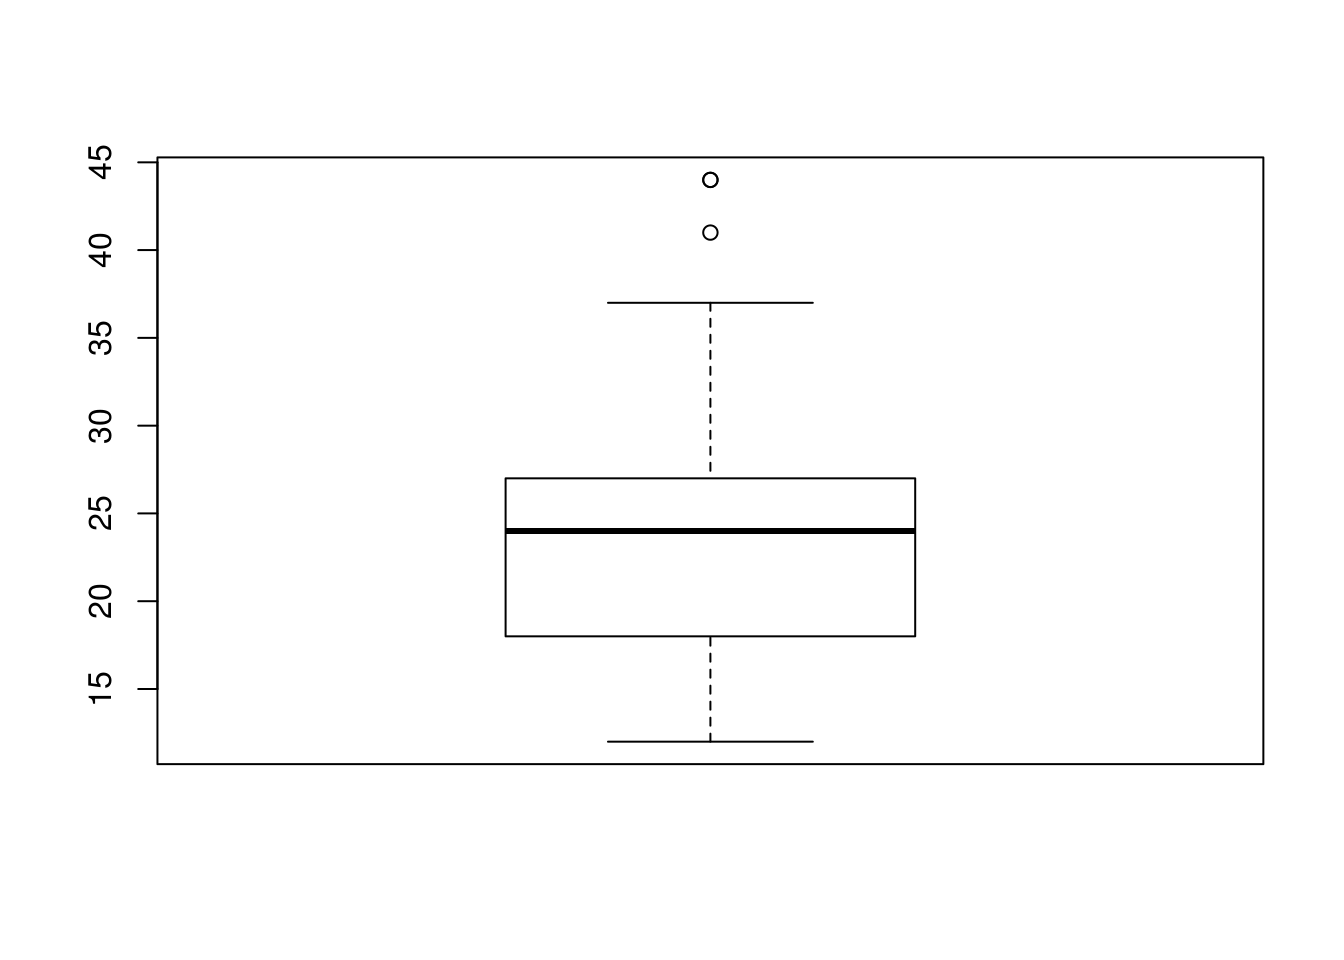
\includegraphics{ScPoEconometrics_files/figure-latex/unnamed-chunk-83-1} \end{center}

Again, \texttt{boxplot()} has a number of additional arguments which
have the ability to make our plot more visually appealing.

\subsection{Scatterplots}\label{scatterplots}

Lastly, to visualize the relationship between two numeric variables we
will use a \textbf{scatterplot}. This can be done with the
\texttt{plot()} function and the \texttt{\textasciitilde{}} syntax we
just used with a boxplot. (The function \texttt{plot()} can also be used
more generally; see the documentation for details.)

\begin{Shaded}
\begin{Highlighting}[]
\KeywordTok{plot}\NormalTok{(hwy }\OperatorTok{~}\StringTok{ }\NormalTok{displ, }\DataTypeTok{data =}\NormalTok{ mpg)}
\end{Highlighting}
\end{Shaded}

\begin{center}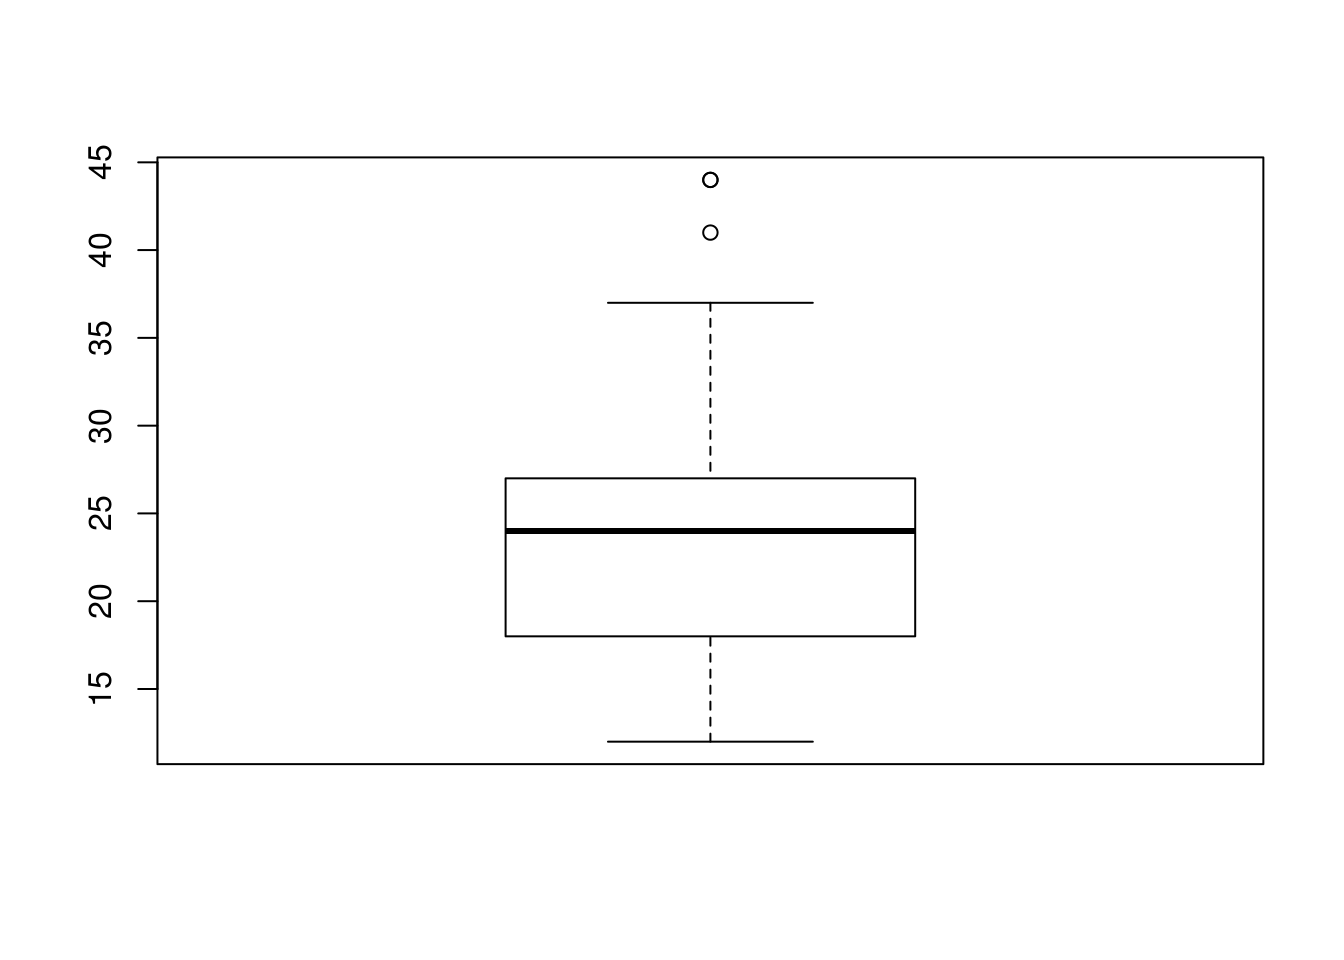
\includegraphics{ScPoEconometrics_files/figure-latex/unnamed-chunk-84-1} \end{center}

\begin{Shaded}
\begin{Highlighting}[]
\KeywordTok{plot}\NormalTok{(hwy }\OperatorTok{~}\StringTok{ }\NormalTok{displ, }\DataTypeTok{data =}\NormalTok{ mpg,}
     \DataTypeTok{xlab =} \StringTok{"Engine Displacement (in Liters)"}\NormalTok{,}
     \DataTypeTok{ylab =} \StringTok{"Miles Per Gallon (Highway)"}\NormalTok{,}
     \DataTypeTok{main =} \StringTok{"MPG (Highway) vs Engine Displacement"}\NormalTok{,}
     \DataTypeTok{pch  =} \DecValTok{20}\NormalTok{,}
     \DataTypeTok{cex  =} \DecValTok{2}\NormalTok{,}
     \DataTypeTok{col  =} \StringTok{"dodgerblue"}\NormalTok{)}
\end{Highlighting}
\end{Shaded}

\begin{center}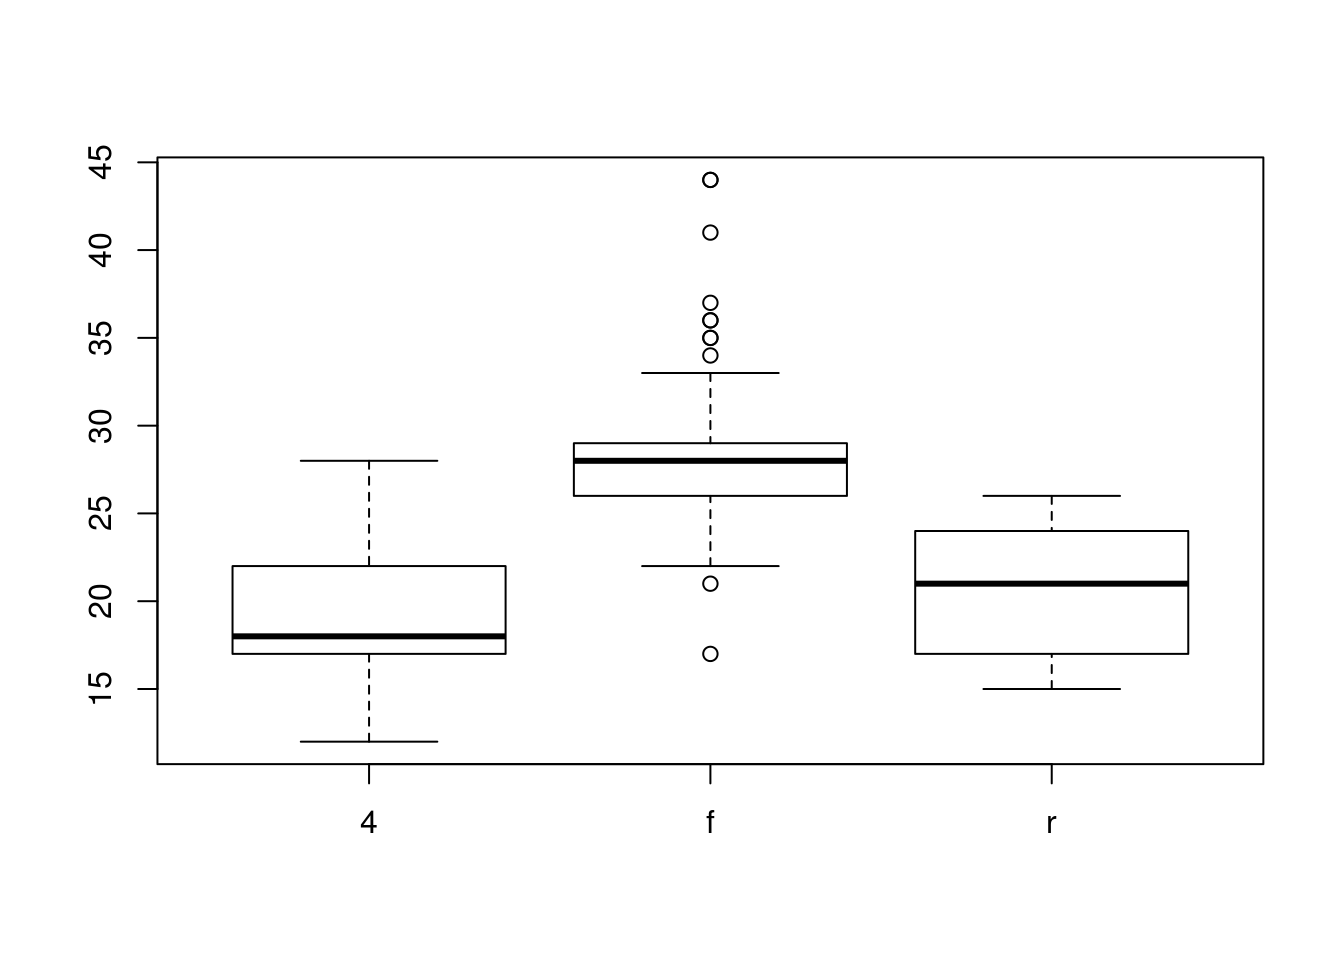
\includegraphics{ScPoEconometrics_files/figure-latex/unnamed-chunk-85-1} \end{center}

\subsection{\texorpdfstring{\texttt{ggplot}}{ggplot}}\label{ggplot}

All of the above plots could also have been generated using the
\texttt{ggplot} function from the already loaded \texttt{ggplot2}
package. Which function you use is up to you, but sometimes a plot is
easier to build in base R (like in the \texttt{boxplot} example maybe),
sometimes the other way around.

\begin{Shaded}
\begin{Highlighting}[]
\KeywordTok{ggplot}\NormalTok{(}\DataTypeTok{data =}\NormalTok{ mpg,}\DataTypeTok{mapping =} \KeywordTok{aes}\NormalTok{(}\DataTypeTok{x=}\NormalTok{displ,}\DataTypeTok{y=}\NormalTok{hwy)) }\OperatorTok{+}\StringTok{ }\KeywordTok{geom_point}\NormalTok{()}
\end{Highlighting}
\end{Shaded}

\begin{center}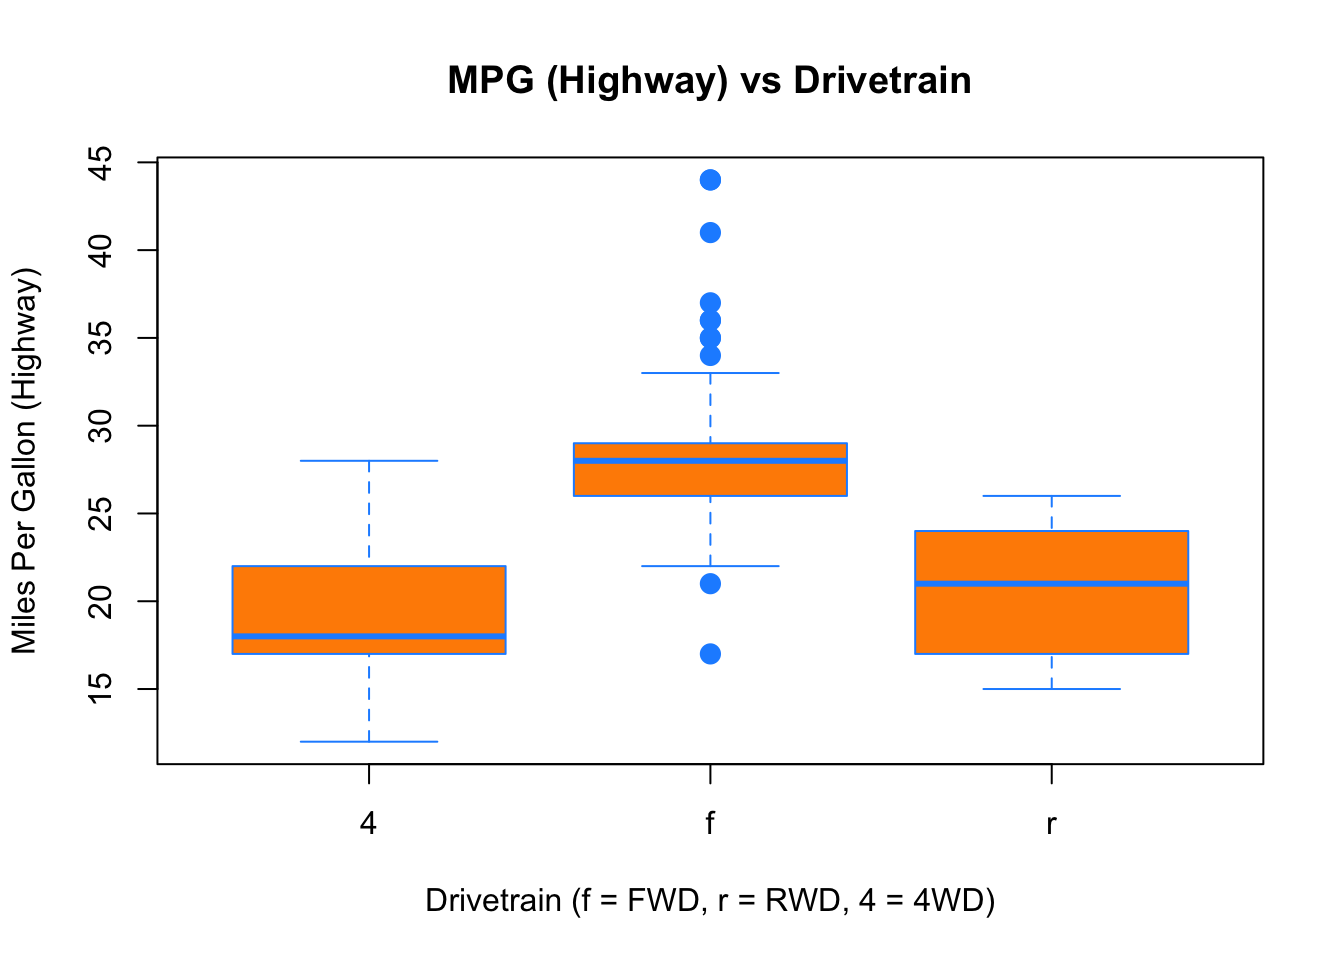
\includegraphics{ScPoEconometrics_files/figure-latex/unnamed-chunk-86-1} \end{center}

\texttt{ggplot} is impossible to describe in brief terms, so please look
at \href{http://ggplot2.tidyverse.org}{the package's website} which
provides excellent guidance. We will from time to time use ggplot in
this book, so you could familiarize yourself with it. Let's quickly
demonstrate how one could further customize that first plot:

\begin{Shaded}
\begin{Highlighting}[]
\KeywordTok{ggplot}\NormalTok{(}\DataTypeTok{data =}\NormalTok{ mpg, }\DataTypeTok{mapping =} \KeywordTok{aes}\NormalTok{(}\DataTypeTok{x=}\NormalTok{displ,}\DataTypeTok{y=}\NormalTok{hwy)) }\OperatorTok{+}\StringTok{   }\CommentTok{# ggplot() makes base plot}
\StringTok{  }\KeywordTok{geom_point}\NormalTok{(}\DataTypeTok{color=}\StringTok{"blue"}\NormalTok{,}\DataTypeTok{size=}\DecValTok{2}\NormalTok{) }\OperatorTok{+}\StringTok{     }\CommentTok{# how to show x and y?}
\StringTok{  }\KeywordTok{scale_y_continuous}\NormalTok{(}\DataTypeTok{name=}\StringTok{"Miles Per Gallon (Highway)"}\NormalTok{) }\OperatorTok{+}\StringTok{  }\CommentTok{# name of y axis}
\StringTok{  }\KeywordTok{scale_x_continuous}\NormalTok{(}\DataTypeTok{name=}\StringTok{"Engine Displacement (in Liters)"}\NormalTok{) }\OperatorTok{+}\StringTok{ }\CommentTok{# x axis}
\StringTok{  }\KeywordTok{theme_bw}\NormalTok{() }\OperatorTok{+}\StringTok{    }\CommentTok{# change the background}
\StringTok{  }\KeywordTok{ggtitle}\NormalTok{(}\StringTok{"MPG (Highway) vs Engine Displacement"}\NormalTok{)   }\CommentTok{# add a title}
\end{Highlighting}
\end{Shaded}

\begin{center}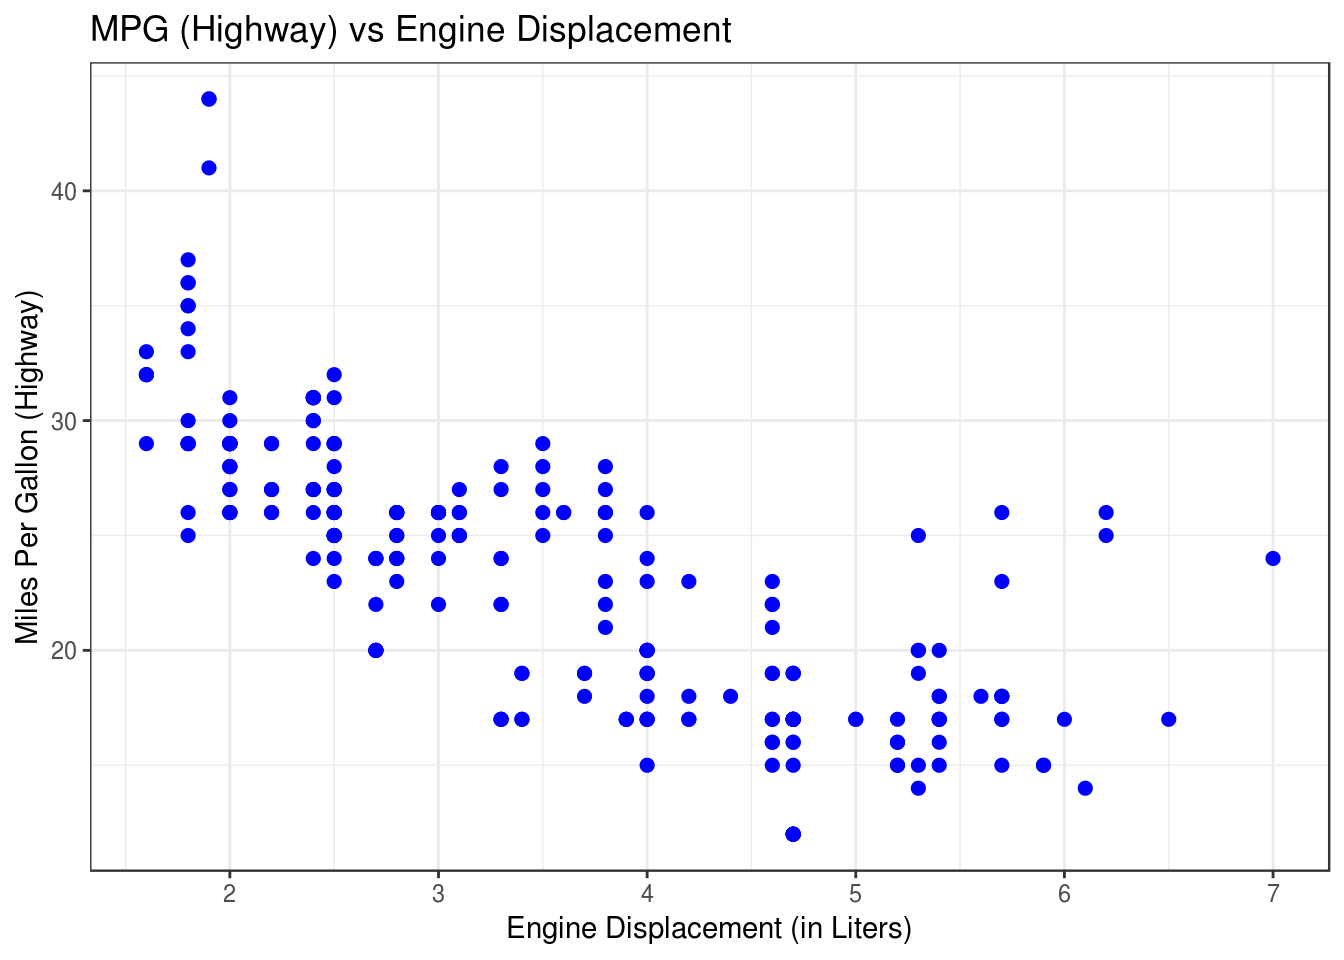
\includegraphics{ScPoEconometrics_files/figure-latex/unnamed-chunk-87-1} \end{center}

If you want to see \texttt{ggplot} in action, you could start with
\href{http://jcyhong.github.io/ggplot_demo.html}{this} and then look at
that
\href{https://tutorials.iq.harvard.edu/R/Rgraphics/Rgraphics.html}{very
nice tutorial}? It's fun!

\section{Summarizing Two Variables}\label{summarize-two}

We often are interested in how two variables are related to each other.
The core concepts here are \emph{covariance} and \emph{correlation}.
Let's generate some data on \texttt{x} and \texttt{y} and plot them
against each other:

\begin{figure}

{\centering 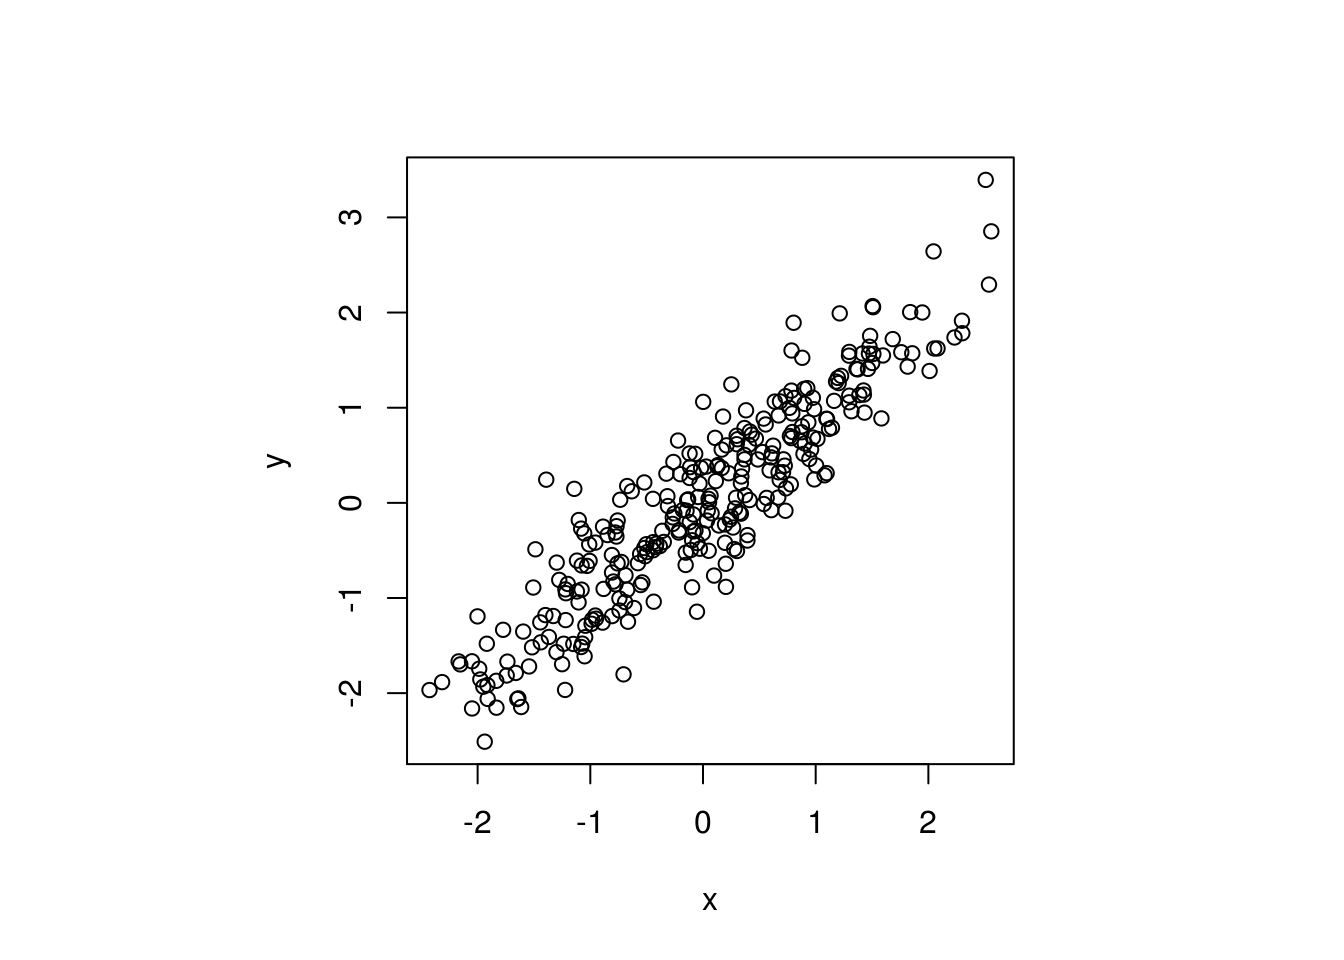
\includegraphics{ScPoEconometrics_files/figure-latex/x-y-corr-1} 

}

\caption{How are $x$ and $y$ related?}\label{fig:x-y-corr}
\end{figure}

Taking as example the data in this plot, the concepts \emph{covariance}
and \emph{correlation} relate to the following type of question:

\begin{note}
Given we observe value of something like \(x=2\), say, can we expect a
high or a low value of \(y\), on average? Something like \(y=2\) or
rather something like \(y=-2\)?
\end{note}

 The answer to this type of question can be addressed by computing the
covariance of both variables:

\begin{Shaded}
\begin{Highlighting}[]
\KeywordTok{cov}\NormalTok{(x,y)  }
\end{Highlighting}
\end{Shaded}

\begin{verbatim}
#OUT> [1] 1.041195
\end{verbatim}

Here, this gives a positive number, 1.04, indicating that as one
variable lies above it's average, the other one does as well. In other
words, it indicates a \textbf{positive relationship}. What is less
clear, however, how to interpret the magnitude of 1.04. Is that a
\emph{strong} or a \emph{weak} positive association?

In fact, we cannot tell. This is because the covariance is measured in
the same units as the data, and those units often differ between both
variables. There is a better measure available to us though, the
\textbf{correlation}, which is obtained by \emph{standardizing} each
variable. By \emph{standardizing} a variable \(x\) one means to divide
\(x\) by its standard deviation \(\sigma_x\):

\[
z = \frac{x}{\sigma_x}
\]

The \emph{correlation coefficient} between \(x\) and \(y\), commonly
denoted \(r_{x,y}\), is then defined as

\[
r_{x,y} = \frac{cov(x,y)}{\sigma_x \sigma_y},
\]

and we get rid of the units problem. In \texttt{R}, you can call
directly

\begin{Shaded}
\begin{Highlighting}[]
\KeywordTok{cor}\NormalTok{(x,y)}
\end{Highlighting}
\end{Shaded}

\begin{verbatim}
#OUT> [1] 0.9142495
\end{verbatim}

Now this is better. Given that the correlation has to lie in \([-1,1]\),
a value of 0.91 is indicative of a rather strong positive relationship
for the data in figure \ref{fig:x-y-corr}

Note that \(x,y\) being drawn from a \emph{continuous distribution}
(they are joint normally distributed) had no implication for covariance
and correlation: We can compute those measures also for discrete random
variables (like the throws of two dice, as you will see in one of our
tutorials).

\subsection{\texorpdfstring{Visually estimating
\(\sigma\)}{Visually estimating \textbackslash{}sigma}}\label{visually-estimating-sigma}

Sometimes it is useful to estimate the standard deviation of some data
\emph{without} the help of a computer (for example during an exam ;-) ).
If \(x\) is approximately normally distributed, 95\% of its observations
will lie within a range of \(\bar{x}\pm\) two standard deviations of
\(x\). That is to say, \emph{four} standard deviations of \(x\) cover
95\% of its observations. Hence, a simple way to estimate the standard
deviation for a variable is to look at the range of \(x\), and simply
divide that number by four.

\begin{figure}

{\centering 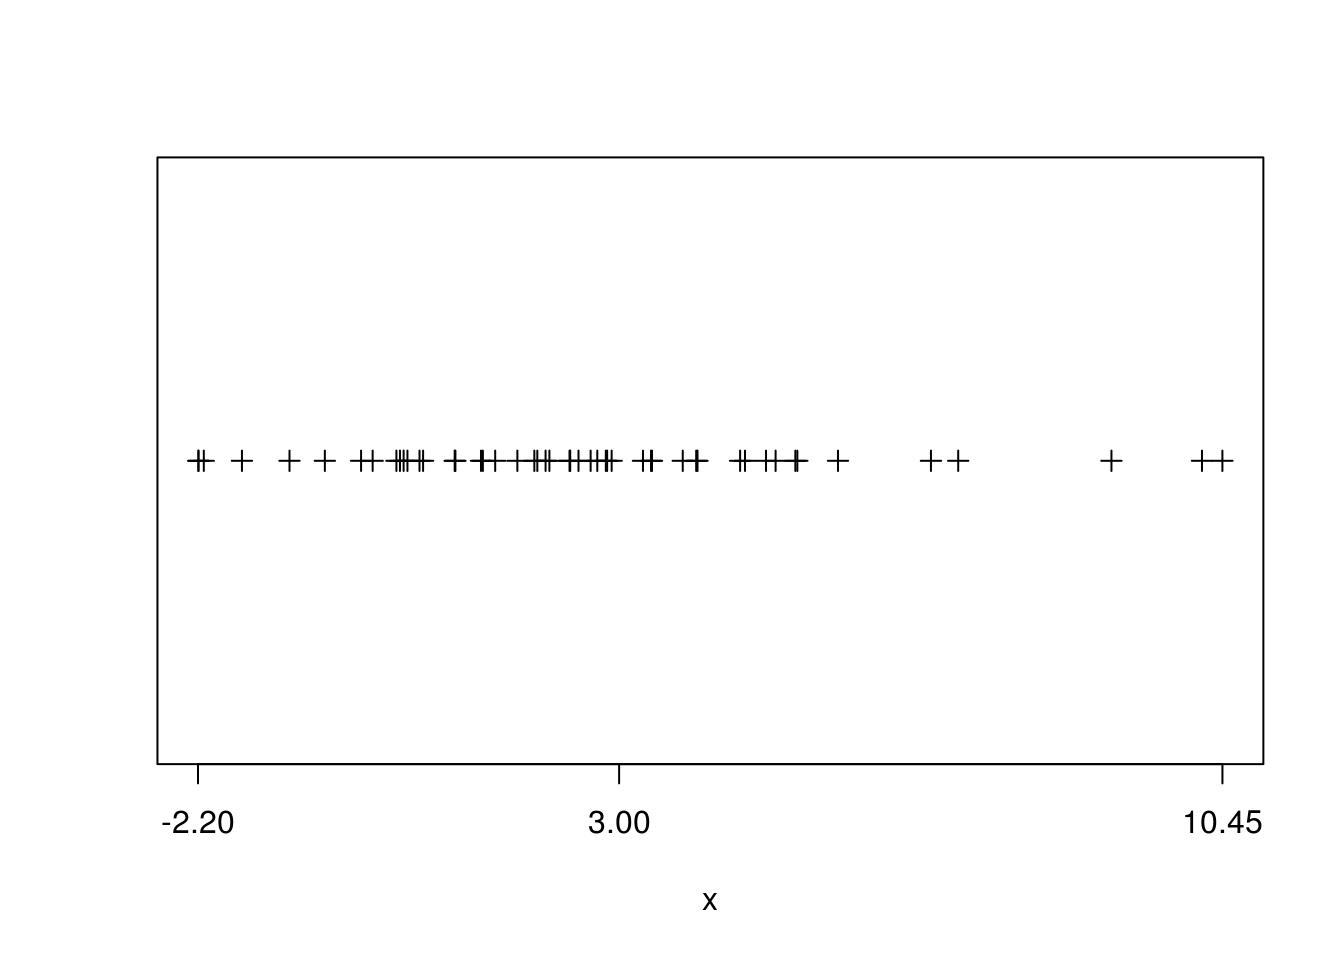
\includegraphics{ScPoEconometrics_files/figure-latex/vis-1} 

}

\caption{visual estimation on $\sigma$. The x-axis labels min and max as well as mean of $x$.}\label{fig:vis}
\end{figure}

This is illustrated in figure \ref{fig:vis}. Here we see that
\texttt{range(x)/4} gives 3.16 which compares favourably to the actual
standard deviation 3.

\section{\texorpdfstring{The
\texttt{tidyverse}}{The tidyverse}}\label{the-tidyverse}

\href{http://hadley.nz}{Hadley Wickham} is the author of R packages
\texttt{ggplot2} and also of \texttt{dplyr} (and also a myriad of
others). With \texttt{ggplot2} he introduced what is called the
\emph{grammar of graphics} (hence, \texttt{gg}) to \texttt{R}. Grammar
in the sense that there are \textbf{nouns} and \textbf{verbs} and a
\textbf{syntax}, i.e.~rules of how nouns and verbs are to be put
together to construct an understandable sentence. He has extended the
\emph{grammar} idea into various other packages. The \texttt{tidyverse}
package is a collection of those packages.

\texttt{tidy} data is data where:

\begin{itemize}
\tightlist
\item
  Each variable is a column
\item
  Each observation is a row
\item
  Each value is a cell
\end{itemize}

Fair enough, you might say, that is a regular spreadsheet. And you are
right! However, data comes to us \emph{not} tidy most of the times, and
we first need to clean, or \texttt{tidy}, it up. Once it's in
\texttt{tidy} format, we can use the tools in the \texttt{tidyverse}
with great efficiency to analyse the data and stop worrying about which
tool to use.

\subsection{\texorpdfstring{Reading \texttt{.csv} data in the
\emph{tidy}
way}{Reading .csv data in the tidy way}}\label{reading-.csv-data-in-the-tidy-way}

We could have used the \texttt{read\_csv()} function from the
\texttt{readr} package to read our example dataset from the previous
chapter. The \texttt{readr} function \texttt{read\_csv()} has a number
of advantages over the built-in \texttt{read.csv}. For example, it is
much faster reading larger data.
\href{https://cran.r-project.org/web/packages/tibble/vignettes/tibble.html}{It
also uses the \texttt{tibble} package to read the data as a tibble.}
\textbf{A \texttt{tibble} is simply a data frame that prints with
sanity.} Notice in the output below that we are given additional
information such as dimension and variable type.

\begin{Shaded}
\begin{Highlighting}[]
\KeywordTok{library}\NormalTok{(readr)  }\CommentTok{# you need `install.packages("readr")` once!}
\NormalTok{path =}\StringTok{ }\KeywordTok{system.file}\NormalTok{(}\DataTypeTok{package=}\StringTok{"ScPoEconometrics"}\NormalTok{,}\StringTok{"datasets"}\NormalTok{,}\StringTok{"example-data.csv"}\NormalTok{)}
\NormalTok{example_data_from_disk =}\StringTok{ }\KeywordTok{read_csv}\NormalTok{(path)}
\end{Highlighting}
\end{Shaded}

\subsection{\texorpdfstring{Tidy \texttt{data.frames} are
\texttt{tibbles}}{Tidy data.frames are tibbles}}\label{tidy-data.frames-are-tibbles}

Let's grab some data from the \texttt{ggplot2} package:

\begin{Shaded}
\begin{Highlighting}[]
\KeywordTok{data}\NormalTok{(mpg,}\DataTypeTok{package =} \StringTok{"ggplot2"}\NormalTok{)  }\CommentTok{# load dataset `mpg` from `ggplot2` package}
\KeywordTok{head}\NormalTok{(mpg, }\DataTypeTok{n =} \DecValTok{10}\NormalTok{)}
\end{Highlighting}
\end{Shaded}

\begin{verbatim}
#OUT> # A tibble: 10 x 11
#OUT>    manufacturer model displ  year   cyl trans drv     cty   hwy fl    cla~
#OUT>    <chr>        <chr> <dbl> <int> <int> <chr> <chr> <int> <int> <chr> <ch>
#OUT>  1 audi         a4      1.8  1999     4 auto~ f        18    29 p     com~
#OUT>  2 audi         a4      1.8  1999     4 manu~ f        21    29 p     com~
#OUT>  3 audi         a4      2    2008     4 manu~ f        20    31 p     com~
#OUT>  4 audi         a4      2    2008     4 auto~ f        21    30 p     com~
#OUT>  5 audi         a4      2.8  1999     6 auto~ f        16    26 p     com~
#OUT>  6 audi         a4      2.8  1999     6 manu~ f        18    26 p     com~
#OUT>  7 audi         a4      3.1  2008     6 auto~ f        18    27 p     com~
#OUT>  8 audi         a4 q~   1.8  1999     4 manu~ 4        18    26 p     com~
#OUT>  9 audi         a4 q~   1.8  1999     4 auto~ 4        16    25 p     com~
#OUT> 10 audi         a4 q~   2    2008     4 manu~ 4        20    28 p     com~
\end{verbatim}

The function \texttt{head()} will display the first \texttt{n}
observations of the data frame, as we have seen. The \texttt{head()}
function was more useful before tibbles. Notice that \texttt{mpg} is a
tibble already, so the output from \texttt{head()} indicates there are
only \texttt{10} observations. Note that this applies to
\texttt{head(mpg,\ n\ =\ 10)} and not \texttt{mpg} itself. Also note
that tibbles print a limited number of rows and columns by default. The
last line of the printed output indicates with rows and columns were
omitted.

\begin{Shaded}
\begin{Highlighting}[]
\NormalTok{mpg}
\end{Highlighting}
\end{Shaded}

\begin{verbatim}
#OUT> # A tibble: 234 x 11
#OUT>    manufacturer model displ  year   cyl trans drv     cty   hwy fl    cla~
#OUT>    <chr>        <chr> <dbl> <int> <int> <chr> <chr> <int> <int> <chr> <ch>
#OUT>  1 audi         a4      1.8  1999     4 auto~ f        18    29 p     com~
#OUT>  2 audi         a4      1.8  1999     4 manu~ f        21    29 p     com~
#OUT>  3 audi         a4      2    2008     4 manu~ f        20    31 p     com~
#OUT>  4 audi         a4      2    2008     4 auto~ f        21    30 p     com~
#OUT>  5 audi         a4      2.8  1999     6 auto~ f        16    26 p     com~
#OUT>  6 audi         a4      2.8  1999     6 manu~ f        18    26 p     com~
#OUT>  7 audi         a4      3.1  2008     6 auto~ f        18    27 p     com~
#OUT>  8 audi         a4 q~   1.8  1999     4 manu~ 4        18    26 p     com~
#OUT>  9 audi         a4 q~   1.8  1999     4 auto~ 4        16    25 p     com~
#OUT> 10 audi         a4 q~   2    2008     4 manu~ 4        20    28 p     com~
#OUT> # ... with 224 more rows
\end{verbatim}

Let's look at \texttt{str} as well to get familiar with the content of
the data:

\begin{Shaded}
\begin{Highlighting}[]
\KeywordTok{str}\NormalTok{(mpg)}
\end{Highlighting}
\end{Shaded}

\begin{verbatim}
#OUT> Classes 'tbl_df', 'tbl' and 'data.frame': 234 obs. of  11 variables:
#OUT>  $ manufacturer: chr  "audi" "audi" "audi" "audi" ...
#OUT>  $ model       : chr  "a4" "a4" "a4" "a4" ...
#OUT>  $ displ       : num  1.8 1.8 2 2 2.8 2.8 3.1 1.8 1.8 2 ...
#OUT>  $ year        : int  1999 1999 2008 2008 1999 1999 2008 1999 1999 2008 ...
#OUT>  $ cyl         : int  4 4 4 4 6 6 6 4 4 4 ...
#OUT>  $ trans       : chr  "auto(l5)" "manual(m5)" "manual(m6)" "auto(av)" ...
#OUT>  $ drv         : chr  "f" "f" "f" "f" ...
#OUT>  $ cty         : int  18 21 20 21 16 18 18 18 16 20 ...
#OUT>  $ hwy         : int  29 29 31 30 26 26 27 26 25 28 ...
#OUT>  $ fl          : chr  "p" "p" "p" "p" ...
#OUT>  $ class       : chr  "compact" "compact" "compact" "compact" ...
\end{verbatim}

In this dataset an observation is for a particular model-year of a car,
and the variables describe attributes of the car, for example its
highway fuel efficiency.

To understand more about the data set, we use the \texttt{?} operator to
pull up the documentation for the data.

\begin{Shaded}
\begin{Highlighting}[]
\NormalTok{?mpg}
\end{Highlighting}
\end{Shaded}

Working with tibbles is mostly the same as working with plain
data.frames:

\begin{Shaded}
\begin{Highlighting}[]
\KeywordTok{names}\NormalTok{(mpg)}
\end{Highlighting}
\end{Shaded}

\begin{verbatim}
#OUT>  [1] "manufacturer" "model"        "displ"        "year"        
#OUT>  [5] "cyl"          "trans"        "drv"          "cty"         
#OUT>  [9] "hwy"          "fl"           "class"
\end{verbatim}

\begin{Shaded}
\begin{Highlighting}[]
\NormalTok{mpg}\OperatorTok{$}\NormalTok{year}
\end{Highlighting}
\end{Shaded}

\begin{verbatim}
#OUT>   [1] 1999 1999 2008 2008 1999 1999 2008 1999 1999 2008 2008 1999 1999 2008
#OUT>  [15] 2008 1999 2008 2008 2008 2008 2008 1999 2008 1999 1999 2008 2008 2008
#OUT>  [29] 2008 2008 1999 1999 1999 2008 1999 2008 2008 1999 1999 1999 1999 2008
#OUT>  [43] 2008 2008 1999 1999 2008 2008 2008 2008 1999 1999 2008 2008 2008 1999
#OUT>  [57] 1999 1999 2008 2008 2008 1999 2008 1999 2008 2008 2008 2008 2008 2008
#OUT>  [71] 1999 1999 2008 1999 1999 1999 2008 1999 1999 1999 2008 2008 1999 1999
#OUT>  [85] 1999 1999 1999 2008 1999 2008 1999 1999 2008 2008 1999 1999 2008 2008
#OUT>  [99] 2008 1999 1999 1999 1999 1999 2008 2008 2008 2008 1999 1999 2008 2008
#OUT> [113] 1999 1999 2008 1999 1999 2008 2008 2008 2008 2008 2008 2008 1999 1999
#OUT> [127] 2008 2008 2008 2008 1999 2008 2008 1999 1999 1999 2008 1999 2008 2008
#OUT> [141] 1999 1999 1999 2008 2008 2008 2008 1999 1999 2008 1999 1999 2008 2008
#OUT> [155] 1999 1999 1999 2008 2008 1999 1999 2008 2008 2008 2008 1999 1999 1999
#OUT> [169] 1999 2008 2008 2008 2008 1999 1999 1999 1999 2008 2008 1999 1999 2008
#OUT> [183] 2008 1999 1999 2008 1999 1999 2008 2008 1999 1999 2008 1999 1999 1999
#OUT> [197] 2008 2008 1999 2008 1999 1999 2008 1999 1999 2008 2008 1999 1999 2008
#OUT> [211] 2008 1999 1999 1999 1999 2008 2008 2008 2008 1999 1999 1999 1999 1999
#OUT> [225] 1999 2008 2008 1999 1999 2008 2008 1999 1999 2008
\end{verbatim}

\begin{Shaded}
\begin{Highlighting}[]
\NormalTok{mpg}\OperatorTok{$}\NormalTok{hwy}
\end{Highlighting}
\end{Shaded}

\begin{verbatim}
#OUT>   [1] 29 29 31 30 26 26 27 26 25 28 27 25 25 25 25 24 25 23 20 15 20 17 17
#OUT>  [24] 26 23 26 25 24 19 14 15 17 27 30 26 29 26 24 24 22 22 24 24 17 22 21
#OUT>  [47] 23 23 19 18 17 17 19 19 12 17 15 17 17 12 17 16 18 15 16 12 17 17 16
#OUT>  [70] 12 15 16 17 15 17 17 18 17 19 17 19 19 17 17 17 16 16 17 15 17 26 25
#OUT>  [93] 26 24 21 22 23 22 20 33 32 32 29 32 34 36 36 29 26 27 30 31 26 26 28
#OUT> [116] 26 29 28 27 24 24 24 22 19 20 17 12 19 18 14 15 18 18 15 17 16 18 17
#OUT> [139] 19 19 17 29 27 31 32 27 26 26 25 25 17 17 20 18 26 26 27 28 25 25 24
#OUT> [162] 27 25 26 23 26 26 26 26 25 27 25 27 20 20 19 17 20 17 29 27 31 31 26
#OUT> [185] 26 28 27 29 31 31 26 26 27 30 33 35 37 35 15 18 20 20 22 17 19 18 20
#OUT> [208] 29 26 29 29 24 44 29 26 29 29 29 29 23 24 44 41 29 26 28 29 29 29 28
#OUT> [231] 29 26 26 26
\end{verbatim}

Subsetting is also similar to dataframe. Here, we find fuel efficient
vehicles earning over 35 miles per gallon and only display
\texttt{manufacturer}, \texttt{model} and \texttt{year}.

\begin{Shaded}
\begin{Highlighting}[]
\CommentTok{# mpg[row condition, col condition]}
\NormalTok{mpg[mpg}\OperatorTok{$}\NormalTok{hwy }\OperatorTok{>}\StringTok{ }\DecValTok{35}\NormalTok{, }\KeywordTok{c}\NormalTok{(}\StringTok{"manufacturer"}\NormalTok{, }\StringTok{"model"}\NormalTok{, }\StringTok{"year"}\NormalTok{)]}
\end{Highlighting}
\end{Shaded}

\begin{verbatim}
#OUT> # A tibble: 6 x 3
#OUT>   manufacturer model       year
#OUT>   <chr>        <chr>      <int>
#OUT> 1 honda        civic       2008
#OUT> 2 honda        civic       2008
#OUT> 3 toyota       corolla     2008
#OUT> 4 volkswagen   jetta       1999
#OUT> 5 volkswagen   new beetle  1999
#OUT> 6 volkswagen   new beetle  1999
\end{verbatim}

An alternative would be to use the \texttt{subset()} function, which has
a much more readable syntax.

\begin{Shaded}
\begin{Highlighting}[]
\KeywordTok{subset}\NormalTok{(mpg, }\DataTypeTok{subset =}\NormalTok{ hwy }\OperatorTok{>}\StringTok{ }\DecValTok{35}\NormalTok{, }\DataTypeTok{select =} \KeywordTok{c}\NormalTok{(}\StringTok{"manufacturer"}\NormalTok{, }\StringTok{"model"}\NormalTok{, }\StringTok{"year"}\NormalTok{))}
\end{Highlighting}
\end{Shaded}

Lastly, and most \emph{tidy}, we could use the \texttt{filter} and
\texttt{select} functions from the \texttt{dplyr} package which
introduces the \emph{pipe operator}
\texttt{f(x)\ \%\textgreater{}\%\ g(z)} from the \texttt{magrittr}
package. This operator takes the output of the first command, for
example \texttt{y\ =\ f(x)}, and passes it \emph{as the first argument}
to the next function, i.e.~we'd obtain \texttt{g(y,z)} here.\footnote{A
  \emph{pipe} is a concept from the Unix world, where it means to take
  the output of some command, and pass it on to another command. This
  way, one can construct a \emph{pipeline} of commands. For additional
  info on the pipe operator in R, you might be interested
  \href{https://www.datacamp.com/community/tutorials/pipe-r-tutorial}{in
  this tutorial}.}

\begin{Shaded}
\begin{Highlighting}[]
\KeywordTok{library}\NormalTok{(dplyr)}
\NormalTok{mpg }\OperatorTok\StringTok{ }
\StringTok{  }\KeywordTok{filter}\NormalTok{(hwy }\OperatorTok{>}\StringTok{ }\DecValTok{35}\NormalTok{) }\OperatorTok\StringTok{ }
\StringTok{  }\KeywordTok{select}\NormalTok{(manufacturer, model, year)}
\end{Highlighting}
\end{Shaded}

\begin{verbatim}
#OUT> # A tibble: 6 x 3
#OUT>   manufacturer model       year
#OUT>   <chr>        <chr>      <int>
#OUT> 1 honda        civic       2008
#OUT> 2 honda        civic       2008
#OUT> 3 toyota       corolla     2008
#OUT> 4 volkswagen   jetta       1999
#OUT> 5 volkswagen   new beetle  1999
#OUT> 6 volkswagen   new beetle  1999
\end{verbatim}

Note that the above syntax is equivalent to the following pipe-free
command (which is much harder to read!):

\begin{Shaded}
\begin{Highlighting}[]
\KeywordTok{library}\NormalTok{(dplyr)}
\KeywordTok{select}\NormalTok{(}\KeywordTok{filter}\NormalTok{(mpg, hwy }\OperatorTok{>}\StringTok{ }\DecValTok{35}\NormalTok{), manufacturer, model, year)}
\end{Highlighting}
\end{Shaded}

\begin{verbatim}
#OUT> # A tibble: 6 x 3
#OUT>   manufacturer model       year
#OUT>   <chr>        <chr>      <int>
#OUT> 1 honda        civic       2008
#OUT> 2 honda        civic       2008
#OUT> 3 toyota       corolla     2008
#OUT> 4 volkswagen   jetta       1999
#OUT> 5 volkswagen   new beetle  1999
#OUT> 6 volkswagen   new beetle  1999
\end{verbatim}

All three approaches produce the same results. Which you use will be
largely based on a given situation as well as your preference.

\subsubsection{Task 1}\label{task-1-1}

\begin{enumerate}
\def\labelenumi{\arabic{enumi}.}
\tightlist
\item
  Make sure to have the \texttt{mpg} dataset loaded by typing
  \texttt{data(mpg)} (and \texttt{library(ggplot2)} if you haven't!).
  Use the \texttt{table} function to find out how many cars were built
  by \emph{mercury}?
\item
  What is the average year the audi's were built in this dataset? Use
  the function \texttt{mean} on the subset of column \texttt{year} that
  corresponds to \texttt{audi}. (Be careful: subsetting a
  \texttt{tibble} returns a \texttt{tibble} (and not a vector)!. so get
  the \texttt{year} column after you have subset the \texttt{tibble}.)
\item
  Use the \texttt{dplyr} piping syntax from above first with
  \texttt{group\_by} and then with
  \texttt{summarise(newvar=your\_expression)} to find the mean
  \texttt{year} by all manufacturers (i.e.~same as previous task, but
  for all manufacturers. don't write a loop!).
\end{enumerate}

\subsection{Tidy Example: Importing Non-Tidy Excel
Data}\label{tidy-example-importing-non-tidy-excel-data}

The data we will look at is from
\href{http://ec.europa.eu/eurostat/data/database}{Eurostat} on
demography and migration. You should download the data yourself (click
on previous link, then drill down to \emph{database by themes
\textgreater{} Population and social conditions \textgreater{} Demograph
and migration \textgreater{} Population change - Demographic balance and
crude rates at national level (demo\_gind)}).

Once downloaded, we can read the data with the function
\texttt{read\_excel} from the package
\href{http://readxl.tidyverse.org}{\texttt{readxl}}, again part of the
\texttt{tidyverse} suite.

It's important to know how the data is organized in the spreadsheet.
Open the file with Excel to see:

\begin{itemize}
\tightlist
\item
  There is a heading which we don't need.
\item
  There are 5 rows with info that we don't need.
\item
  There is one table per variable (total population, males, females,
  etc)
\item
  Each table has one row for each country, and one column for each year.
\item
  As such, this data is \textbf{not tidy}.
\end{itemize}

Now we will read the first chunk of data, from the first table:
\emph{total population}:

\begin{Shaded}
\begin{Highlighting}[]
\KeywordTok{library}\NormalTok{(readxl)  }\CommentTok{# load the library}
\CommentTok{# Notice that if you installed the R package of this book,}
\CommentTok{# you have the .xls data file already at }
\CommentTok{# `system.file(package="ScPoEconometrics",}
\CommentTok{#                        "datasets","demo_gind.xls")`}
\CommentTok{# otherwise:}
\CommentTok{# * download the file to your computer}
\CommentTok{# * change the argument `path` to where you downloaded it}
\CommentTok{# you may want to change your working directory with `setwd("your/directory")}
\CommentTok{# or in RStudio by clicking Session > Set Working Directory}

\CommentTok{# total population in raw format}
\NormalTok{tot_pop_raw =}\StringTok{ }\KeywordTok{read_excel}\NormalTok{(}
                \DataTypeTok{path =} \KeywordTok{system.file}\NormalTok{(}\DataTypeTok{package=}\StringTok{"ScPoEconometrics"}\NormalTok{,}
                                    \StringTok{"datasets"}\NormalTok{,}\StringTok{"demo_gind.xls"}\NormalTok{), }
                \DataTypeTok{sheet=}\StringTok{"Data"}\NormalTok{, }\CommentTok{# which sheet}
                \DataTypeTok{range=}\StringTok{"A9:K68"}\NormalTok{)  }\CommentTok{# which excel cell range to read}
\KeywordTok{names}\NormalTok{(tot_pop_raw)[}\DecValTok{1}\NormalTok{] <-}\StringTok{ "Country"}   \CommentTok{# lets rename the first column}
\NormalTok{tot_pop_raw}
\end{Highlighting}
\end{Shaded}

\begin{verbatim}
#OUT> # A tibble: 59 x 11
#OUT>    Country `2008` `2009` `2010` `2011` `2012` `2013` `2014` `2015` `2016`
#OUT>    <chr>   <chr>  <chr>  <chr>  <chr>  <chr>  <chr>  <chr>  <chr>  <chr> 
#OUT>  1 Europe~ 50029~ 50209~ 50317~ 50296~ 50404~ 50516~ 50701~ 50854~ 51027~
#OUT>  2 Europe~ 43872~ 44004~ 44066~ 43994~ 44055~ 44125~ 44266~ 44366~ 44489~
#OUT>  3 Europe~ 49598~ 49778~ 49886~ 49867~ 49977~ 50090~ 50276~ 50431~ 50608~
#OUT>  4 Euro a~ 33309~ 33447~ 33526~ 33457~ 33528~ 33604~ 33754~ 33856~ 33988~
#OUT>  5 Euro a~ 32988~ 33128~ 33212~ 33152~ 33228~ 33307~ 33459~ 33563~ 33699~
#OUT>  6 Belgium 10666~ 10753~ 10839~ 11000~ 11075~ 11137~ 11180~ 11237~ 11311~
#OUT>  7 Bulgar~ 75180~ 74671~ 74217~ 73694~ 73272~ 72845~ 72456~ 72021~ 71537~
#OUT>  8 Czech ~ 10343~ 10425~ 10462~ 10486~ 10505~ 10516~ 10512~ 10538~ 10553~
#OUT>  9 Denmark 54757~ 55114~ 55347~ 55606~ 55805~ 56026~ 56272~ 56597~ 57072~
#OUT> 10 German~ 82217~ 82002~ 81802~ 80222~ 80327~ 80523~ 80767~ 81197~ 82175~
#OUT> # ... with 49 more rows, and 1 more variable: `2017` <chr>
\end{verbatim}

This shows a \texttt{tibble}, which we encountered just above. The
column names are \texttt{Country,2008,2009,...}, and the rows are
numbered \texttt{1,2,3,...}. Notice, in particular, that \emph{all}
columns seem to be of type \texttt{\textless{}chr\textgreater{}},
i.e.~characters - a string, not a number! We'll have to fix that, as
this is clearly numeric data.

\subsubsection{\texorpdfstring{\texttt{tidyr}}{tidyr}}\label{tidyr}

In the previous \texttt{tibble}, each year is a column name (like
\texttt{2008}) instead of all years being collected in one column
\texttt{year}. We really would like to have several rows for each
Country, one row per year. We want to \texttt{gather()} all years into a
new column to tidy this up - and here is how:

\begin{enumerate}
\def\labelenumi{\arabic{enumi}.}
\tightlist
\item
  specify which columns are to be gathered: in our case, all years (note
  that \texttt{paste(2008:2017)} produces a vector like
  \texttt{{[}"2008",\ "2009",\ "2010",...{]}})
\item
  say what those columns should be gathered into, i.e.~what is the
  \emph{key} for those values: we'll call it \texttt{year}.
\item
  Finally, what is the name of the new resulting column, containing the
  \emph{value} from each cell: let's call it \texttt{counts}.
\end{enumerate}

\begin{Shaded}
\begin{Highlighting}[]
\KeywordTok{library}\NormalTok{(tidyr)   }\CommentTok{# for the gather function}
\NormalTok{tot_pop =}\StringTok{ }\KeywordTok{gather}\NormalTok{(tot_pop_raw, }\KeywordTok{paste}\NormalTok{(}\DecValTok{2008}\OperatorTok{:}\DecValTok{2017}\NormalTok{),}\DataTypeTok{key=}\StringTok{"year"}\NormalTok{, }\DataTypeTok{value =} \StringTok{"counts"}\NormalTok{)}
\NormalTok{tot_pop}
\end{Highlighting}
\end{Shaded}

\begin{verbatim}
#OUT> # A tibble: 590 x 3
#OUT>    Country                                          year  counts   
#OUT>    <chr>                                            <chr> <chr>    
#OUT>  1 European Union (current composition)             2008  500297033
#OUT>  2 European Union (without United Kingdom)          2008  438725386
#OUT>  3 European Union (before the accession of Croatia) 2008  495985066
#OUT>  4 Euro area (19 countries)                         2008  333096775
#OUT>  5 Euro area (18 countries)                         2008  329884170
#OUT>  6 Belgium                                          2008  10666866 
#OUT>  7 Bulgaria                                         2008  7518002  
#OUT>  8 Czech Republic                                   2008  10343422 
#OUT>  9 Denmark                                          2008  5475791  
#OUT> 10 Germany (until 1990 former territory of the FRG) 2008  82217837 
#OUT> # ... with 580 more rows
\end{verbatim}

That's better! However, \texttt{counts} is still \texttt{chr}! Let's
convert it to a number:

\begin{Shaded}
\begin{Highlighting}[]
\NormalTok{tot_pop}\OperatorTok{$}\NormalTok{counts =}\StringTok{ }\KeywordTok{as.integer}\NormalTok{(tot_pop}\OperatorTok{$}\NormalTok{counts)}
\end{Highlighting}
\end{Shaded}

\begin{verbatim}
#OUT> Warning: NAs introduced by coercion
\end{verbatim}

\begin{Shaded}
\begin{Highlighting}[]
\NormalTok{tot_pop}
\end{Highlighting}
\end{Shaded}

\begin{verbatim}
#OUT> # A tibble: 590 x 3
#OUT>    Country                                          year     counts
#OUT>    <chr>                                            <chr>     <int>
#OUT>  1 European Union (current composition)             2008  500297033
#OUT>  2 European Union (without United Kingdom)          2008  438725386
#OUT>  3 European Union (before the accession of Croatia) 2008  495985066
#OUT>  4 Euro area (19 countries)                         2008  333096775
#OUT>  5 Euro area (18 countries)                         2008  329884170
#OUT>  6 Belgium                                          2008   10666866
#OUT>  7 Bulgaria                                         2008    7518002
#OUT>  8 Czech Republic                                   2008   10343422
#OUT>  9 Denmark                                          2008    5475791
#OUT> 10 Germany (until 1990 former territory of the FRG) 2008   82217837
#OUT> # ... with 580 more rows
\end{verbatim}

Now you can see that column \texttt{counts} is indeed \texttt{int},
i.e.~an integer number, and we are fine. The
\texttt{Warning:\ NAs\ introduced\ by\ coercion} means that \texttt{R}
converted some values to \texttt{NA}, because it couldn't convert them
into \texttt{numeric}. More below!

\subsubsection{\texorpdfstring{\texttt{dplyr}}{dplyr}}\label{dplyr}

\begin{quote}
The \href{http://r4ds.had.co.nz/transform.html}{transform} chapter of
Hadley Wickham's book is a great place to read up more on using
\texttt{dplyr}.
\end{quote}

With \texttt{dplyr} you can do the following operations on
\texttt{data.frame}s and \texttt{tibble}s:

\begin{itemize}
\tightlist
\item
  Choose observations based on a certain value (i.e.~subset):
  \texttt{filter()}
\item
  Reorder rows: \texttt{arrange()}
\item
  Select variables by name: \texttt{select()}
\item
  Create new variables out of existing ones: \texttt{mutate()}
\item
  Summarise variables: \texttt{summarise()}
\end{itemize}

All of those verbs can be used with \texttt{group\_by()}, where we apply
the respective operation on a \emph{group} of the dataframe/tibble. For
example, on our \texttt{tot\_pop} tibble we will now

\begin{itemize}
\tightlist
\item
  filter
\item
  mutate
\item
  and plot the resulting values
\end{itemize}

Let's get a plot of the populations of France, the UK and Italy over
time, in terms of millions of people. We will make use of the
\texttt{piping} syntax of \texttt{dplyr} which we introduced just above.

\begin{Shaded}
\begin{Highlighting}[]
\KeywordTok{library}\NormalTok{(dplyr)  }\CommentTok{# for %>%, filter, mutate, ...}
\CommentTok{# 1. take the data.frame `tot_pop`}
\NormalTok{tot_pop }\OperatorTok
\StringTok{  }\CommentTok{# 2. pipe it into the filter function}
\StringTok{  }\CommentTok{# filter on Country being one of "France","United Kingdom" or "Italy"}
\StringTok{  }\KeywordTok{filter}\NormalTok{(Country }\OperatorTok\StringTok{ }\KeywordTok{c}\NormalTok{(}\StringTok{"France"}\NormalTok{,}\StringTok{"United Kingdom"}\NormalTok{,}\StringTok{"Italy"}\NormalTok{)) }\OperatorTok
\StringTok{  }\CommentTok{# 3. pipe the result into the mutate function}
\StringTok{  }\CommentTok{# create a new column called millions}
\StringTok{  }\KeywordTok{mutate}\NormalTok{(}\DataTypeTok{millions =}\NormalTok{ counts }\OperatorTok{/}\StringTok{ }\FloatTok{1e6}\NormalTok{) }\OperatorTok
\StringTok{  }\CommentTok{# 4. pipe the result into ggplot to make a plot}
\StringTok{  }\KeywordTok{ggplot}\NormalTok{(}\DataTypeTok{mapping =} \KeywordTok{aes}\NormalTok{(}\DataTypeTok{x=}\NormalTok{year,}\DataTypeTok{y=}\NormalTok{millions,}\DataTypeTok{color=}\NormalTok{Country,}\DataTypeTok{group=}\NormalTok{Country)) }\OperatorTok{+}\StringTok{ }\KeywordTok{geom_line}\NormalTok{(}\DataTypeTok{size=}\DecValTok{1}\NormalTok{)}
\end{Highlighting}
\end{Shaded}

\begin{center}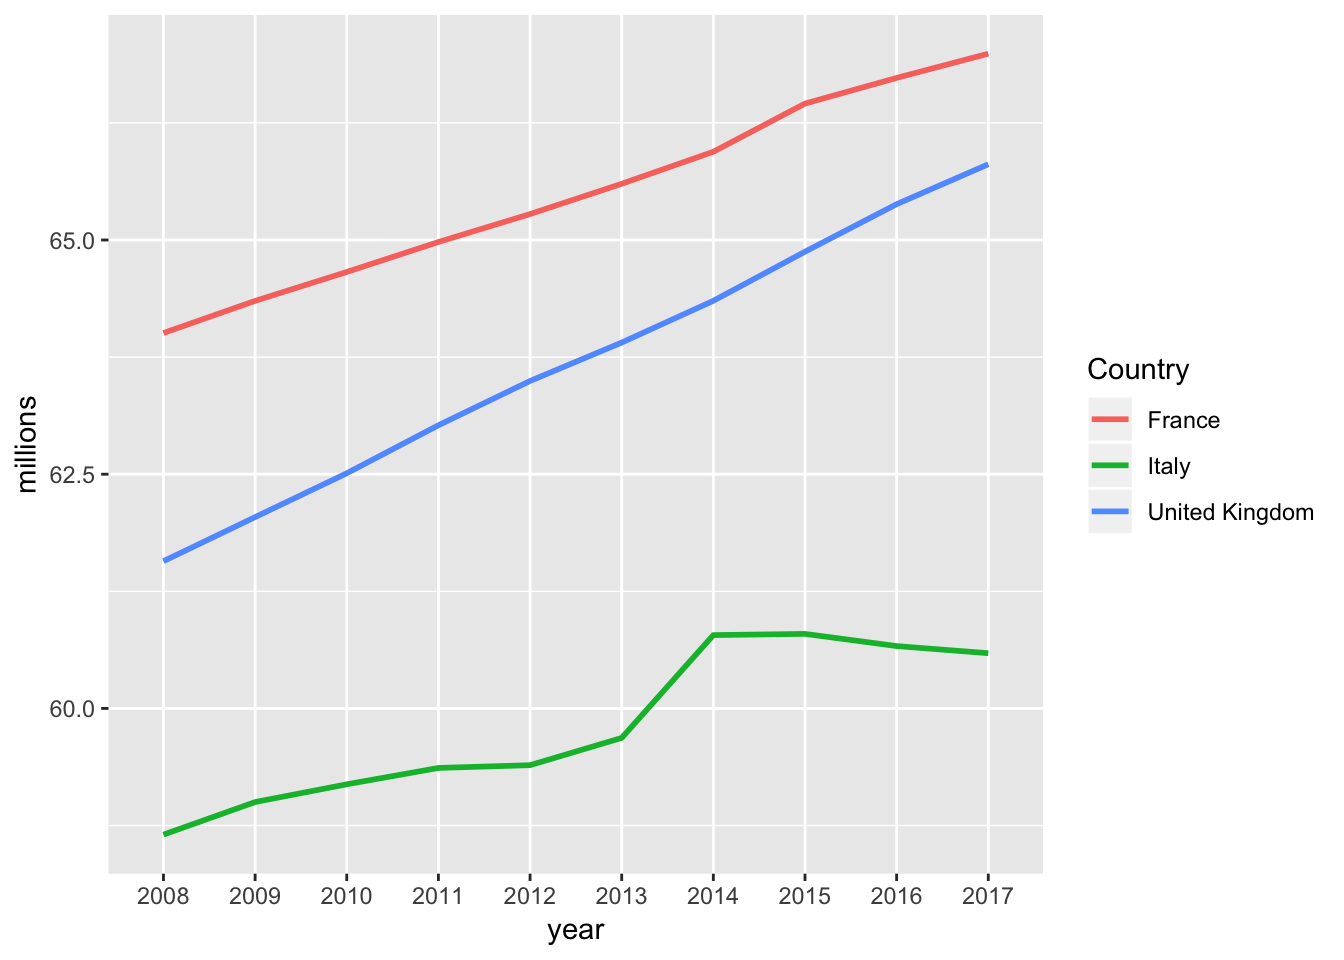
\includegraphics{ScPoEconometrics_files/figure-latex/gather-plot-1} \end{center}

\subsubsection*{\texorpdfstring{Arrange a
\texttt{tibble}}{Arrange a tibble}}\label{arrange-a-tibble}
\addcontentsline{toc}{subsubsection}{Arrange a \texttt{tibble}}

\begin{itemize}
\tightlist
\item
  What are the top/bottom 5 most populated areas?
\end{itemize}

\begin{Shaded}
\begin{Highlighting}[]
\NormalTok{top5 =}\StringTok{ }\NormalTok{tot_pop }\OperatorTok
\StringTok{  }\KeywordTok{arrange}\NormalTok{(}\KeywordTok{desc}\NormalTok{(counts)) }\OperatorTok\StringTok{  }\CommentTok{# arrange in descending order of col `counts`}
\StringTok{  }\KeywordTok{top_n}\NormalTok{(}\DecValTok{5}\NormalTok{)}

\NormalTok{bottom5 =}\StringTok{ }\NormalTok{tot_pop }\OperatorTok
\StringTok{  }\KeywordTok{arrange}\NormalTok{(}\KeywordTok{desc}\NormalTok{(counts)) }\OperatorTok
\StringTok{  }\KeywordTok{top_n}\NormalTok{(}\OperatorTok{-}\DecValTok{5}\NormalTok{)}
\CommentTok{# let's see top 5}
\NormalTok{top5}
\end{Highlighting}
\end{Shaded}

\begin{verbatim}
#OUT> # A tibble: 5 x 3
#OUT>   Country                                                   year    counts
#OUT>   <chr>                                                     <chr>    <int>
#OUT> 1 European Economic Area (EU28  - current composition, plu~ 2017    5.17e8
#OUT> 2 European Economic Area (EU28  - current composition, plu~ 2016    5.16e8
#OUT> 3 European Economic Area (EU28  - current composition, plu~ 2015    5.14e8
#OUT> 4 European Economic Area (EU27 -  before the accession of ~ 2017    5.13e8
#OUT> 5 European Economic Area (EU28  - current composition, plu~ 2014    5.12e8
\end{verbatim}

\begin{Shaded}
\begin{Highlighting}[]
\CommentTok{# and bottom 5}
\NormalTok{bottom5}
\end{Highlighting}
\end{Shaded}

\begin{verbatim}
#OUT> # A tibble: 5 x 3
#OUT>   Country    year  counts
#OUT>   <chr>      <chr>  <int>
#OUT> 1 San Marino 2015   32789
#OUT> 2 San Marino 2014   32520
#OUT> 3 San Marino 2008   32054
#OUT> 4 San Marino 2011   31863
#OUT> 5 San Marino 2009   31269
\end{verbatim}

Now this is not exactly what we wanted. It's always the same country in
both top and bottom, because there are multiple years per country. Let's
compute average population over the last 5 years and rank according to
that:

\begin{Shaded}
\begin{Highlighting}[]
\NormalTok{topbottom =}\StringTok{ }\NormalTok{tot_pop }\OperatorTok
\StringTok{  }\KeywordTok{group_by}\NormalTok{(Country) }\OperatorTok
\StringTok{  }\KeywordTok{filter}\NormalTok{(year }\OperatorTok{>}\StringTok{ }\DecValTok{2012}\NormalTok{) }\OperatorTok
\StringTok{  }\KeywordTok{summarise}\NormalTok{(}\DataTypeTok{mean_count =} \KeywordTok{mean}\NormalTok{(counts)) }\OperatorTok
\StringTok{  }\KeywordTok{arrange}\NormalTok{(}\KeywordTok{desc}\NormalTok{(mean_count))}

\NormalTok{top5 =}\StringTok{ }\NormalTok{topbottom }\OperatorTok\StringTok{ }\KeywordTok{top_n}\NormalTok{(}\DecValTok{5}\NormalTok{)}
\NormalTok{bottom5 =}\StringTok{ }\NormalTok{topbottom }\OperatorTok\StringTok{ }\KeywordTok{top_n}\NormalTok{(}\OperatorTok{-}\DecValTok{5}\NormalTok{)}
\NormalTok{top5}
\end{Highlighting}
\end{Shaded}

\begin{verbatim}
#OUT> # A tibble: 5 x 2
#OUT>   Country                                                       mean_count
#OUT>   <chr>                                                              <dbl>
#OUT> 1 European Economic Area (EU28  - current composition, plus IS~ 514029320 
#OUT> 2 European Economic Area (EU27 -  before the accession of Croa~ 509813491.
#OUT> 3 European Union (current composition)                          508502858.
#OUT> 4 European Union (before the accession of Croatia)              504287028.
#OUT> 5 European Union (without United Kingdom)                       443638309.
\end{verbatim}

\begin{Shaded}
\begin{Highlighting}[]
\NormalTok{bottom5}
\end{Highlighting}
\end{Shaded}

\begin{verbatim}
#OUT> # A tibble: 5 x 2
#OUT>   Country       mean_count
#OUT>   <chr>              <dbl>
#OUT> 1 Luxembourg       563319.
#OUT> 2 Malta            440467.
#OUT> 3 Iceland          329501.
#OUT> 4 Liechtenstein     37353 
#OUT> 5 San Marino        33014.
\end{verbatim}

That's better!

\subsubsection*{\texorpdfstring{Look for \texttt{NA}s in a
\texttt{tibble}}{Look for NAs in a tibble}}\label{look-for-nas-in-a-tibble}
\addcontentsline{toc}{subsubsection}{Look for \texttt{NA}s in a
\texttt{tibble}}

Sometimes data is \emph{missing}, and \texttt{R} represents it with the
special value \texttt{NA} (not available). It is good to know where in
our dataset we are going to encounter any missing values, so the task
here is: let's produce a table that has three columns:

\begin{enumerate}
\def\labelenumi{\arabic{enumi}.}
\tightlist
\item
  the names of countries with missing data
\item
  how many years of data are missing for each of those
\item
  and the actual years that are missing
\end{enumerate}

\begin{Shaded}
\begin{Highlighting}[]
\NormalTok{missings =}\StringTok{ }\NormalTok{tot_pop }\OperatorTok
\StringTok{  }\KeywordTok{filter}\NormalTok{(}\KeywordTok{is.na}\NormalTok{(counts)) }\OperatorTok\StringTok{ }\CommentTok{# is.na(x) returns TRUE if x is NA}
\StringTok{  }\KeywordTok{group_by}\NormalTok{(Country) }\OperatorTok
\StringTok{  }\KeywordTok{summarise}\NormalTok{(}\DataTypeTok{n_missing =} \KeywordTok{n}\NormalTok{(),}\DataTypeTok{years =} \KeywordTok{paste}\NormalTok{(year,}\DataTypeTok{collapse =} \StringTok{", "}\NormalTok{))}
\NormalTok{knitr}\OperatorTok{:::}\KeywordTok{kable}\NormalTok{(missings)  }\CommentTok{# knitr:::kable makes a nice table}
\end{Highlighting}
\end{Shaded}

\begin{tabular}{l|r|l}
\hline
Country & n\_missing & years\\
\hline
Albania & 2 & 2010, 2012\\
\hline
Andorra & 2 & 2014, 2015\\
\hline
Armenia & 1 & 2014\\
\hline
France (metropolitan) & 4 & 2014, 2015, 2016, 2017\\
\hline
Georgia & 1 & 2013\\
\hline
Monaco & 7 & 2008, 2009, 2010, 2011, 2012, 2013, 2014\\
\hline
Russia & 4 & 2013, 2015, 2016, 2017\\
\hline
San Marino & 1 & 2010\\
\hline
\end{tabular}

\subsubsection*{Males and Females}\label{males-and-females}
\addcontentsline{toc}{subsubsection}{Males and Females}

Let's look at the numbers by male and female population. They are in the
same xls file, but at different cell ranges. Also, I just realised that
the special character \texttt{:} indicates \emph{missing} data. We can
feed that to \texttt{read\_excel} and that will spare us the need to
convert data types afterwards. Let's see:

\begin{Shaded}
\begin{Highlighting}[]
\NormalTok{females_raw =}\StringTok{ }\KeywordTok{read_excel}\NormalTok{(}
                \DataTypeTok{path =} \KeywordTok{system.file}\NormalTok{(}\DataTypeTok{package=}\StringTok{"ScPoEconometrics"}\NormalTok{,}
                                    \StringTok{"datasets"}\NormalTok{,}\StringTok{"demo_gind.xls"}\NormalTok{), }
                \DataTypeTok{sheet=}\StringTok{"Data"}\NormalTok{, }\CommentTok{# which sheet}
                \DataTypeTok{range=}\StringTok{"A141:K200"}\NormalTok{,  }\CommentTok{# which excel cell range to read}
                \DataTypeTok{na=}\StringTok{":"}\NormalTok{ )   }\CommentTok{# missing data indicator}
\KeywordTok{names}\NormalTok{(females_raw)[}\DecValTok{1}\NormalTok{] <-}\StringTok{ "Country"}   \CommentTok{# lets rename the first column}
\NormalTok{females_raw}
\end{Highlighting}
\end{Shaded}

\begin{verbatim}
#OUT> # A tibble: 59 x 11
#OUT>    Country `2008` `2009` `2010` `2011` `2012` `2013` `2014` `2015` `2016`
#OUT>    <chr>    <dbl>  <dbl>  <dbl>  <dbl>  <dbl>  <dbl>  <dbl>  <dbl>  <dbl>
#OUT>  1 Europe~ 2.56e8 2.57e8 2.58e8 2.58e8 2.58e8 2.59e8 2.60e8 2.60e8 2.61e8
#OUT>  2 Europe~ 2.25e8 2.26e8 2.26e8 2.26e8 2.26e8 2.26e8 2.27e8 2.27e8 2.28e8
#OUT>  3 Europe~ 2.54e8 2.55e8 2.55e8 2.56e8 2.56e8 2.57e8 2.57e8 2.58e8 2.59e8
#OUT>  4 Euro a~ 1.71e8 1.71e8 1.72e8 1.72e8 1.72e8 1.72e8 1.73e8 1.73e8 1.74e8
#OUT>  5 Euro a~ 1.69e8 1.70e8 1.70e8 1.70e8 1.70e8 1.71e8 1.71e8 1.72e8 1.72e8
#OUT>  6 Belgium 5.44e6 5.48e6 5.53e6 5.60e6 5.64e6 5.67e6 5.69e6 5.71e6 5.74e6
#OUT>  7 Bulgar~ 3.86e6 3.83e6 3.81e6 3.78e6 3.76e6 3.74e6 3.72e6 3.70e6 3.68e6
#OUT>  8 Czech ~ 5.28e6 5.31e6 5.33e6 5.34e6 5.35e6 5.35e6 5.35e6 5.36e6 5.37e6
#OUT>  9 Denmark 2.76e6 2.78e6 2.79e6 2.80e6 2.81e6 2.82e6 2.83e6 2.85e6 2.87e6
#OUT> 10 German~ 4.19e7 4.18e7 4.17e7 4.11e7 4.11e7 4.11e7 4.12e7 4.14e7 4.17e7
#OUT> # ... with 49 more rows, and 1 more variable: `2017` <dbl>
\end{verbatim}

You can see that \texttt{R} now correctly read the numbers as such,
after we told it that the \texttt{:} character has the special
\emph{missing} meaning: before, it \emph{coerced} the entire
\texttt{2008} column (for example) to be of type \texttt{chr} after it
hit the first \texttt{:}. We had to manually convert the column back to
\texttt{numeric}, in the process automatically coercing the \texttt{:}s
into \texttt{NA}. Now we addressed that issue directly. Let's also get
the male data in the same way:

\begin{Shaded}
\begin{Highlighting}[]
\NormalTok{males_raw =}\StringTok{ }\KeywordTok{read_excel}\NormalTok{(}
                \DataTypeTok{path =} \KeywordTok{system.file}\NormalTok{(}\DataTypeTok{package=}\StringTok{"ScPoEconometrics"}\NormalTok{,}
                                    \StringTok{"datasets"}\NormalTok{,}\StringTok{"demo_gind.xls"}\NormalTok{), }
                \DataTypeTok{sheet=}\StringTok{"Data"}\NormalTok{, }\CommentTok{# which sheet}
                \DataTypeTok{range=}\StringTok{"A75:K134"}\NormalTok{,  }\CommentTok{# which excel cell range to read}
                \DataTypeTok{na=}\StringTok{":"}\NormalTok{ )   }\CommentTok{# missing data indicator}
\KeywordTok{names}\NormalTok{(males_raw)[}\DecValTok{1}\NormalTok{] <-}\StringTok{ "Country"}   \CommentTok{# lets rename the first column}
\end{Highlighting}
\end{Shaded}

Next step was to \texttt{tidy} up this data, just as before:

\begin{Shaded}
\begin{Highlighting}[]
\NormalTok{females =}\StringTok{ }\KeywordTok{gather}\NormalTok{(females_raw, }\KeywordTok{paste}\NormalTok{(}\DecValTok{2008}\OperatorTok{:}\DecValTok{2017}\NormalTok{),}\DataTypeTok{key=}\StringTok{"year"}\NormalTok{, }\DataTypeTok{value =} \StringTok{"counts"}\NormalTok{)}
\NormalTok{males =}\StringTok{ }\KeywordTok{gather}\NormalTok{(males_raw, }\KeywordTok{paste}\NormalTok{(}\DecValTok{2008}\OperatorTok{:}\DecValTok{2017}\NormalTok{),}\DataTypeTok{key=}\StringTok{"year"}\NormalTok{, }\DataTypeTok{value =} \StringTok{"counts"}\NormalTok{)}
\end{Highlighting}
\end{Shaded}

Let's try to tweak our above plot to show the same data in two separate
panels: one for males and one for females. This is easiest to do with
\texttt{ggplot} if we have all the data in one single
\texttt{data.frame} (or \texttt{tibble}), and marked with a \emph{group
identifier}. Let's first add this to both datasets, and then let's just
combine both into one:

\begin{Shaded}
\begin{Highlighting}[]
\NormalTok{females}\OperatorTok{$}\NormalTok{sex =}\StringTok{ "female"}
\NormalTok{males}\OperatorTok{$}\NormalTok{sex =}\StringTok{ "male"}
\NormalTok{sexes =}\StringTok{ }\KeywordTok{rbind}\NormalTok{(males,females)   }\CommentTok{# "row bind" 2 data.frames}
\NormalTok{sexes}
\end{Highlighting}
\end{Shaded}

\begin{verbatim}
#OUT> # A tibble: 1,180 x 4
#OUT>    Country                                          year     counts sex  
#OUT>    <chr>                                            <chr>     <dbl> <chr>
#OUT>  1 European Union (current composition)             2008  243990548 male 
#OUT>  2 European Union (without United Kingdom)          2008  213826199 male 
#OUT>  3 European Union (before the accession of Croatia) 2008  241913560 male 
#OUT>  4 Euro area (19 countries)                         2008  162516883 male 
#OUT>  5 Euro area (18 countries)                         2008  161029464 male 
#OUT>  6 Belgium                                          2008    5224309 male 
#OUT>  7 Bulgaria                                         2008    3660367 male 
#OUT>  8 Czech Republic                                   2008    5065117 male 
#OUT>  9 Denmark                                          2008    2712666 male 
#OUT> 10 Germany (until 1990 former territory of the FRG) 2008   40274292 male 
#OUT> # ... with 1,170 more rows
\end{verbatim}

Now that we have all the data nice and \texttt{tidy} in a
\texttt{data.frame}, this is a very small change to our previous
plotting code:

\begin{Shaded}
\begin{Highlighting}[]
\NormalTok{sexes }\OperatorTok
\StringTok{  }\KeywordTok{filter}\NormalTok{(Country }\OperatorTok\StringTok{ }\KeywordTok{c}\NormalTok{(}\StringTok{"France"}\NormalTok{,}\StringTok{"United Kingdom"}\NormalTok{,}\StringTok{"Italy"}\NormalTok{)) }\OperatorTok
\StringTok{  }\KeywordTok{mutate}\NormalTok{(}\DataTypeTok{millions =}\NormalTok{ counts }\OperatorTok{/}\StringTok{ }\FloatTok{1e6}\NormalTok{) }\OperatorTok
\StringTok{  }\KeywordTok{ggplot}\NormalTok{(}\DataTypeTok{mapping =} \KeywordTok{aes}\NormalTok{(}\DataTypeTok{x=}\KeywordTok{as.Date}\NormalTok{(year,}\DataTypeTok{format=}\StringTok{"%Y"}\NormalTok{),  }\CommentTok{# convert to `Date`}
                       \DataTypeTok{y=}\NormalTok{millions,}\DataTypeTok{colour=}\NormalTok{Country,}\DataTypeTok{group=}\NormalTok{Country)) }\OperatorTok{+}\StringTok{ }
\StringTok{      }\KeywordTok{geom_line}\NormalTok{() }\OperatorTok{+}
\StringTok{  }\KeywordTok{scale_x_date}\NormalTok{(}\DataTypeTok{name =} \StringTok{"year"}\NormalTok{) }\OperatorTok{+}\StringTok{ }\CommentTok{# rename x axis}
\StringTok{  }\KeywordTok{facet_wrap}\NormalTok{(}\OperatorTok{~}\NormalTok{sex)   }\CommentTok{# make two panels, splitting by groups `sex`}
\end{Highlighting}
\end{Shaded}

\begin{center}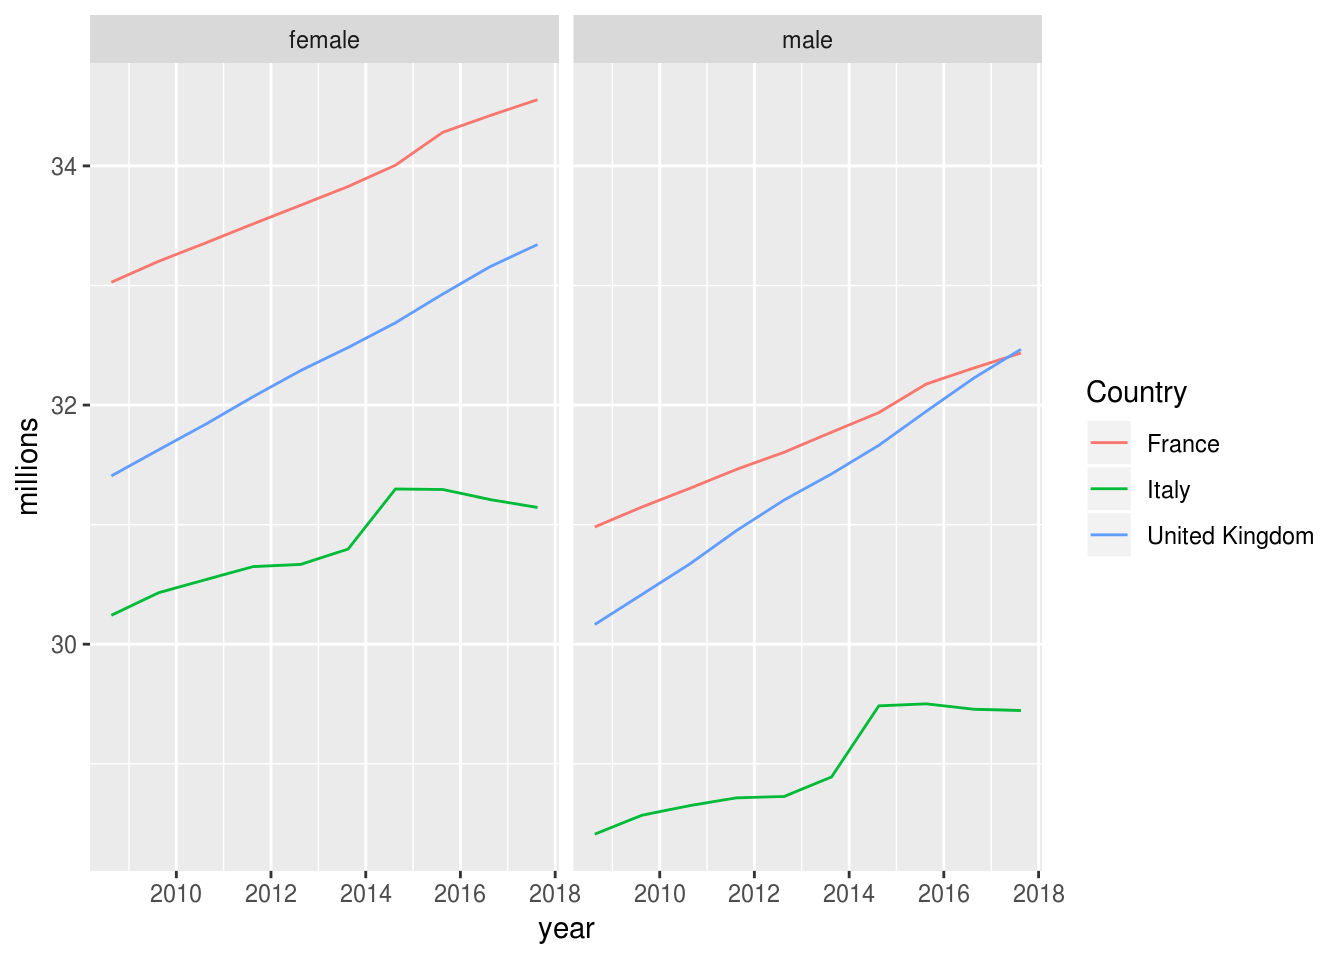
\includegraphics{ScPoEconometrics_files/figure-latex/psexes-1} \end{center}

\subsubsection*{Always Compare to Germany
:-)}\label{always-compare-to-germany--}
\addcontentsline{toc}{subsubsection}{Always Compare to Germany :-)}

How do our three countries compare with respect to the biggest country
in the EU in terms of population? What \emph{fraction} of Germany does
the French population make in any given year, for example?

\begin{Shaded}
\begin{Highlighting}[]
\CommentTok{# remember that the pipe operator %>% takes the }
\CommentTok{# result of the previous operation and passes it}
\CommentTok{# as the *first* argument to the next function call}
\NormalTok{merge_GER <-}\StringTok{ }\NormalTok{tot_pop }\OperatorTok
\StringTok{  }\CommentTok{# 1. subset to countries of interest}
\StringTok{  }\KeywordTok{filter}\NormalTok{(}
\NormalTok{    Country }\OperatorTok\StringTok{ }
\StringTok{      }\KeywordTok{c}\NormalTok{(}\StringTok{"France"}\NormalTok{,}
        \StringTok{"United Kingdom"}\NormalTok{,}
        \StringTok{"Italy"}\NormalTok{)}
\NormalTok{    ) }\OperatorTok
\StringTok{  }\CommentTok{# 2. group data by year}
\StringTok{  }\KeywordTok{group_by}\NormalTok{(year) }\OperatorTok
\StringTok{  }\CommentTok{# 3. add GER's count as new column *by year*}
\StringTok{  }\KeywordTok{left_join}\NormalTok{(}
    \CommentTok{# Germany only}
    \KeywordTok{filter}\NormalTok{(tot_pop,}
\NormalTok{           Country }\OperatorTok\StringTok{ "Germany including former GDR"}\NormalTok{),}
    \CommentTok{# join back in `by year`}
    \DataTypeTok{by=}\StringTok{"year"}\NormalTok{)}
\NormalTok{merge_GER}
\end{Highlighting}
\end{Shaded}

\begin{verbatim}
#OUT> # A tibble: 30 x 5
#OUT> # Groups:   year [?]
#OUT>    Country.x      year  counts.x Country.y                    counts.y
#OUT>    <chr>          <chr>    <int> <chr>                           <int>
#OUT>  1 France         2008  64007193 Germany including former GDR 82217837
#OUT>  2 Italy          2008  58652875 Germany including former GDR 82217837
#OUT>  3 United Kingdom 2008  61571647 Germany including former GDR 82217837
#OUT>  4 France         2009  64350226 Germany including former GDR 82002356
#OUT>  5 Italy          2009  59000586 Germany including former GDR 82002356
#OUT>  6 United Kingdom 2009  62042343 Germany including former GDR 82002356
#OUT>  7 France         2010  64658856 Germany including former GDR 81802257
#OUT>  8 Italy          2010  59190143 Germany including former GDR 81802257
#OUT>  9 United Kingdom 2010  62510197 Germany including former GDR 81802257
#OUT> 10 France         2011  64978721 Germany including former GDR 80222065
#OUT> # ... with 20 more rows
\end{verbatim}

Here you see that the merge (or join) operation labelled \texttt{col.x}
and \texttt{col.y} if both datasets contained a column called
\texttt{col}. Now let's continue to compute what proportion of german
population each country amounts to:

\begin{Shaded}
\begin{Highlighting}[]
\KeywordTok{names}\NormalTok{(merge_GER)[}\DecValTok{1}\NormalTok{] <-}\StringTok{ "Country"}
\NormalTok{merge_GER }\OperatorTok
\StringTok{  }\KeywordTok{mutate}\NormalTok{(}\DataTypeTok{prop_GER =} \DecValTok{100} \OperatorTok{*}\StringTok{ }\NormalTok{counts.x }\OperatorTok{/}\StringTok{ }\NormalTok{counts.y) }\OperatorTok
\StringTok{  }\CommentTok{# 5. plot}
\StringTok{  }\KeywordTok{ggplot}\NormalTok{(}\DataTypeTok{mapping =} 
           \KeywordTok{aes}\NormalTok{(}\DataTypeTok{x =}\NormalTok{ year,}
               \DataTypeTok{y =}\NormalTok{ prop_GER,}
               \DataTypeTok{color =}\NormalTok{ Country,}
               \DataTypeTok{group =}\NormalTok{ Country)) }\OperatorTok{+}\StringTok{ }
\StringTok{  }\KeywordTok{geom_line}\NormalTok{(}\DataTypeTok{size=}\DecValTok{1}\NormalTok{) }\OperatorTok{+}\StringTok{ }
\StringTok{  }\KeywordTok{scale_y_continuous}\NormalTok{(}\StringTok{"percent of German population"}\NormalTok{) }\OperatorTok{+}\StringTok{ }
\StringTok{  }\KeywordTok{theme_bw}\NormalTok{()  }\CommentTok{# new theme for a change?}
\end{Highlighting}
\end{Shaded}

\begin{center}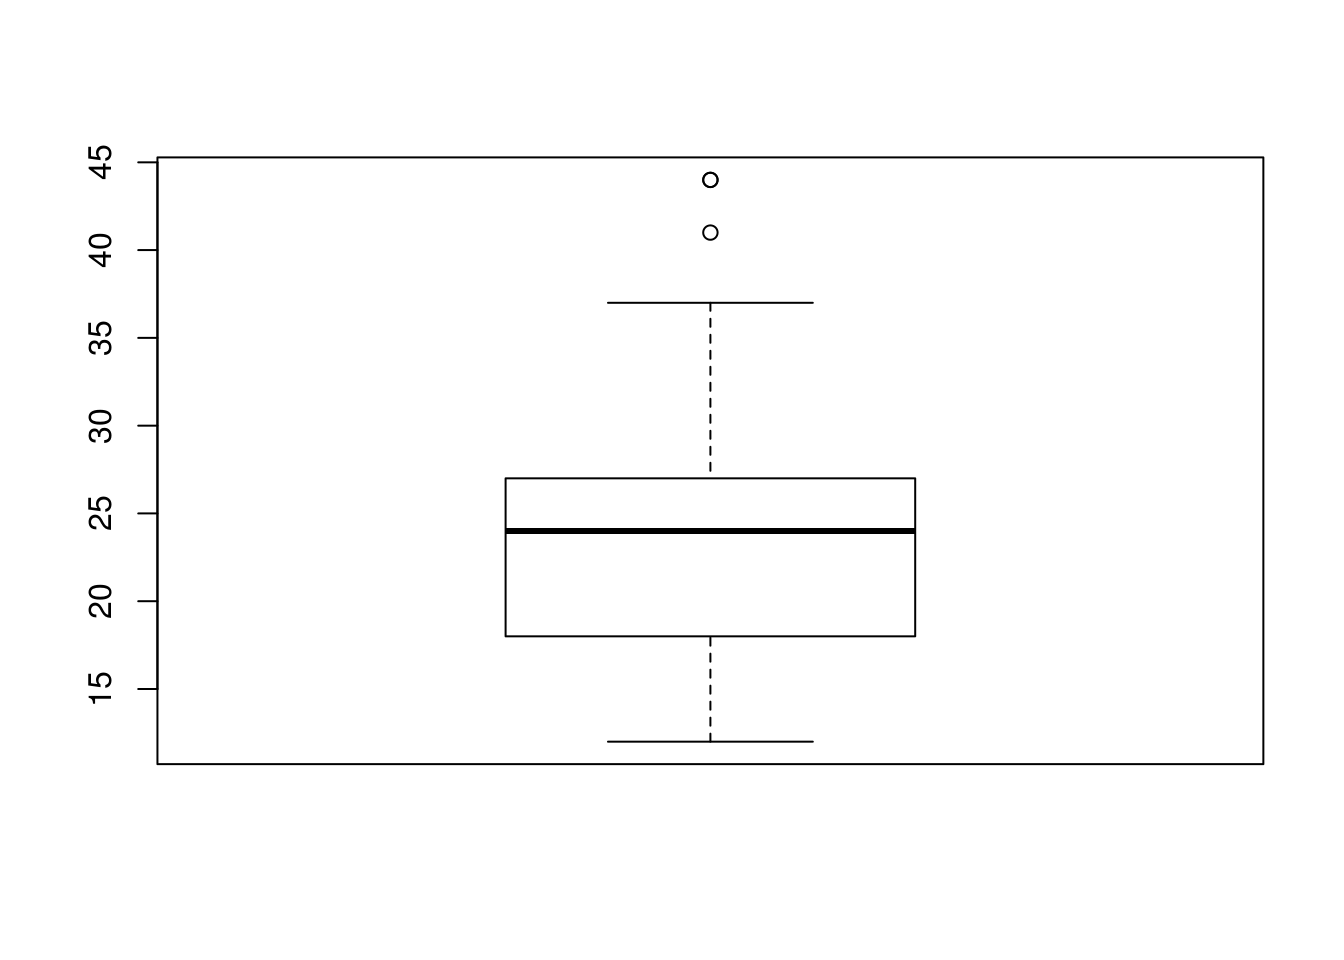
\includegraphics{ScPoEconometrics_files/figure-latex/unnamed-chunk-107-1} \end{center}

\chapter{Linear Regression}\label{linreg}

In this chapter we will learn an additional way how one can represent
the relationship between \emph{outcome}, or \emph{dependent} variable
variable \(y\) and an \emph{explanatory} or \emph{independent} variable
\(x\). We will refer throughout to the graphical representation of a
collection of independent observations on \(x\) and \(y\), i.e., a
\emph{dataset}.

\section{\texorpdfstring{How are \texttt{x} and \texttt{y}
related?}{How are x and y related?}}\label{how-are-x-and-y-related}

\subsection{Data on Cars}\label{data-on-cars}

We will look at the built-in \texttt{cars} dataset. Let's get a view of
this by just typing \texttt{View(cars)} in Rstudio. You can see
something like this:

\begin{verbatim}
#OUT>   speed dist
#OUT> 1     4    2
#OUT> 2     4   10
#OUT> 3     7    4
#OUT> 4     7   22
#OUT> 5     8   16
#OUT> 6     9   10
\end{verbatim}

We have a \texttt{data.frame} with two columns: \texttt{speed} and
\texttt{dist}. Type \texttt{help(cars)} to find out more about the
dataset. There you could read that

\begin{quote}
The data give the speed of cars (mph) and the distances taken to stop
(ft).
\end{quote}

It's good practice to know the extent of a dataset. You could just type

\begin{Shaded}
\begin{Highlighting}[]
\KeywordTok{dim}\NormalTok{(cars)}
\end{Highlighting}
\end{Shaded}

\begin{verbatim}
#OUT> [1] 50  2
\end{verbatim}

to find out that we have 50 rows and 2 columns. A central question that
we want to ask now is the following:

\subsection{\texorpdfstring{How are \texttt{speed} and \texttt{dist}
related?}{How are speed and dist related?}}\label{how-are-speed-and-dist-related}

The simplest way to start is to plot the data. Remembering that we view
each row of a data.frame as an observation, we could just label one axis
of a graph \texttt{speed}, and the other one \texttt{dist}, and go
through our table above row by row. We just have to read off the x/y
coordinates and mark them in the graph. In \texttt{R}:

\begin{Shaded}
\begin{Highlighting}[]
\KeywordTok{plot}\NormalTok{(dist }\OperatorTok{~}\StringTok{ }\NormalTok{speed, }\DataTypeTok{data =}\NormalTok{ cars,}
     \DataTypeTok{xlab =} \StringTok{"Speed (in Miles Per Hour)"}\NormalTok{,}
     \DataTypeTok{ylab =} \StringTok{"Stopping Distance (in Feet)"}\NormalTok{,}
     \DataTypeTok{main =} \StringTok{"Stopping Distance vs Speed"}\NormalTok{,}
     \DataTypeTok{pch  =} \DecValTok{20}\NormalTok{,}
     \DataTypeTok{cex  =} \DecValTok{2}\NormalTok{,}
     \DataTypeTok{col  =} \StringTok{"red"}\NormalTok{)}
\end{Highlighting}
\end{Shaded}

\begin{center}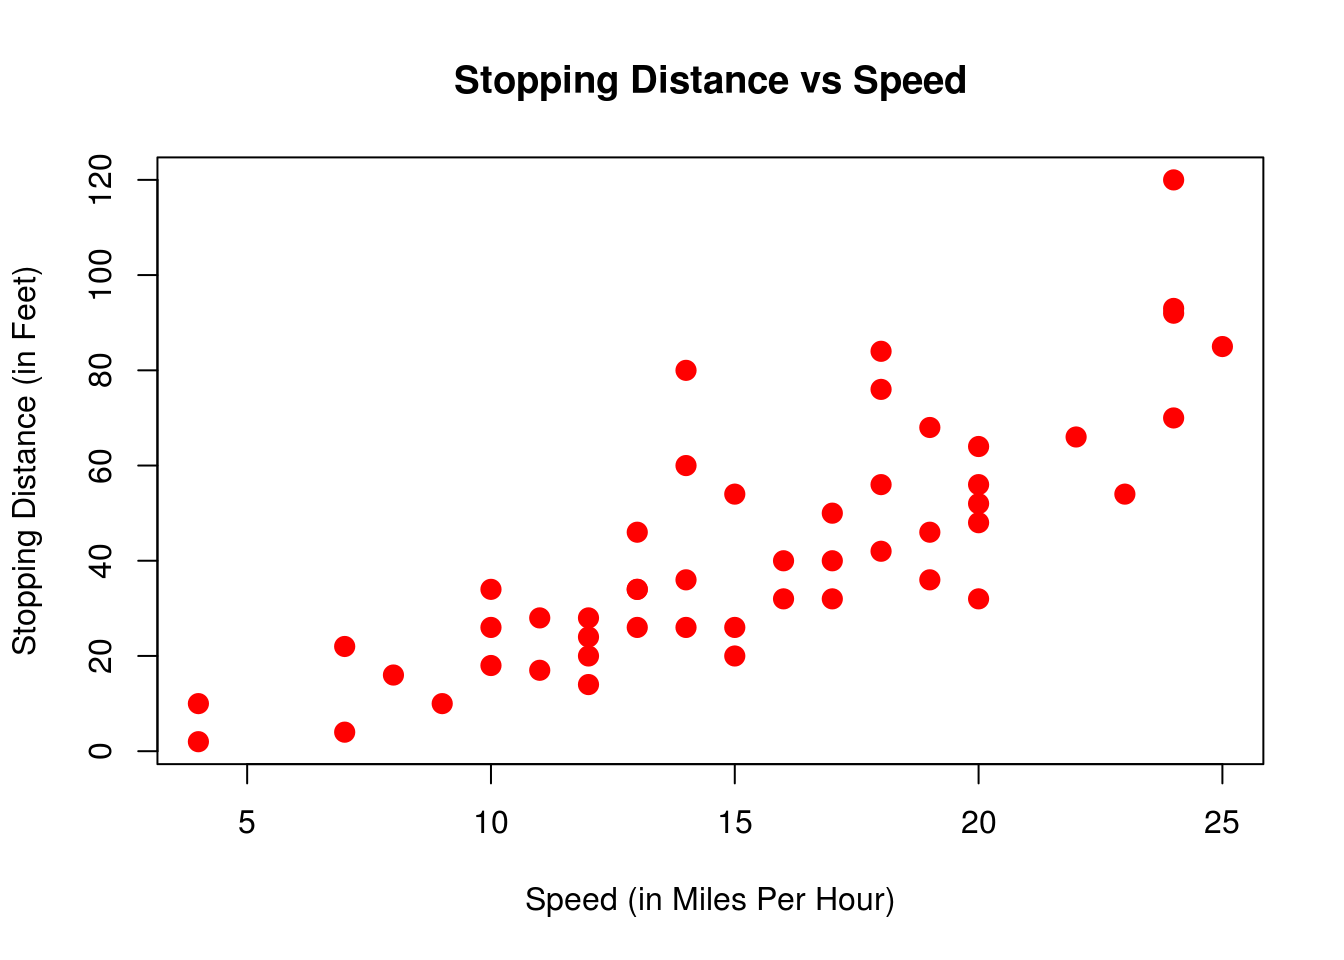
\includegraphics{ScPoEconometrics_files/figure-latex/unnamed-chunk-110-1} \end{center}

Here, each dot represents one observation. In this case, one particular
measurement \texttt{speed} and \texttt{dist} for a car. Now, again:

\begin{note}
How are \texttt{speed} and \texttt{dist} related? How could one best
\emph{summarize} this relationship?
\end{note}

 One thing we could do, is draw a straight line through this
scatterplot, like so:

\begin{Shaded}
\begin{Highlighting}[]
\KeywordTok{plot}\NormalTok{(dist }\OperatorTok{~}\StringTok{ }\NormalTok{speed, }\DataTypeTok{data =}\NormalTok{ cars,}
     \DataTypeTok{xlab =} \StringTok{"Speed (in Miles Per Hour)"}\NormalTok{,}
     \DataTypeTok{ylab =} \StringTok{"Stopping Distance (in Feet)"}\NormalTok{,}
     \DataTypeTok{main =} \StringTok{"Stopping Distance vs Speed"}\NormalTok{,}
     \DataTypeTok{pch  =} \DecValTok{20}\NormalTok{,}
     \DataTypeTok{cex  =} \DecValTok{2}\NormalTok{,}
     \DataTypeTok{col  =} \StringTok{"red"}\NormalTok{)}
\KeywordTok{abline}\NormalTok{(}\DataTypeTok{a =} \DecValTok{60}\NormalTok{,}\DataTypeTok{b =} \DecValTok{0}\NormalTok{,}\DataTypeTok{lw=}\DecValTok{3}\NormalTok{)}
\end{Highlighting}
\end{Shaded}

\begin{center}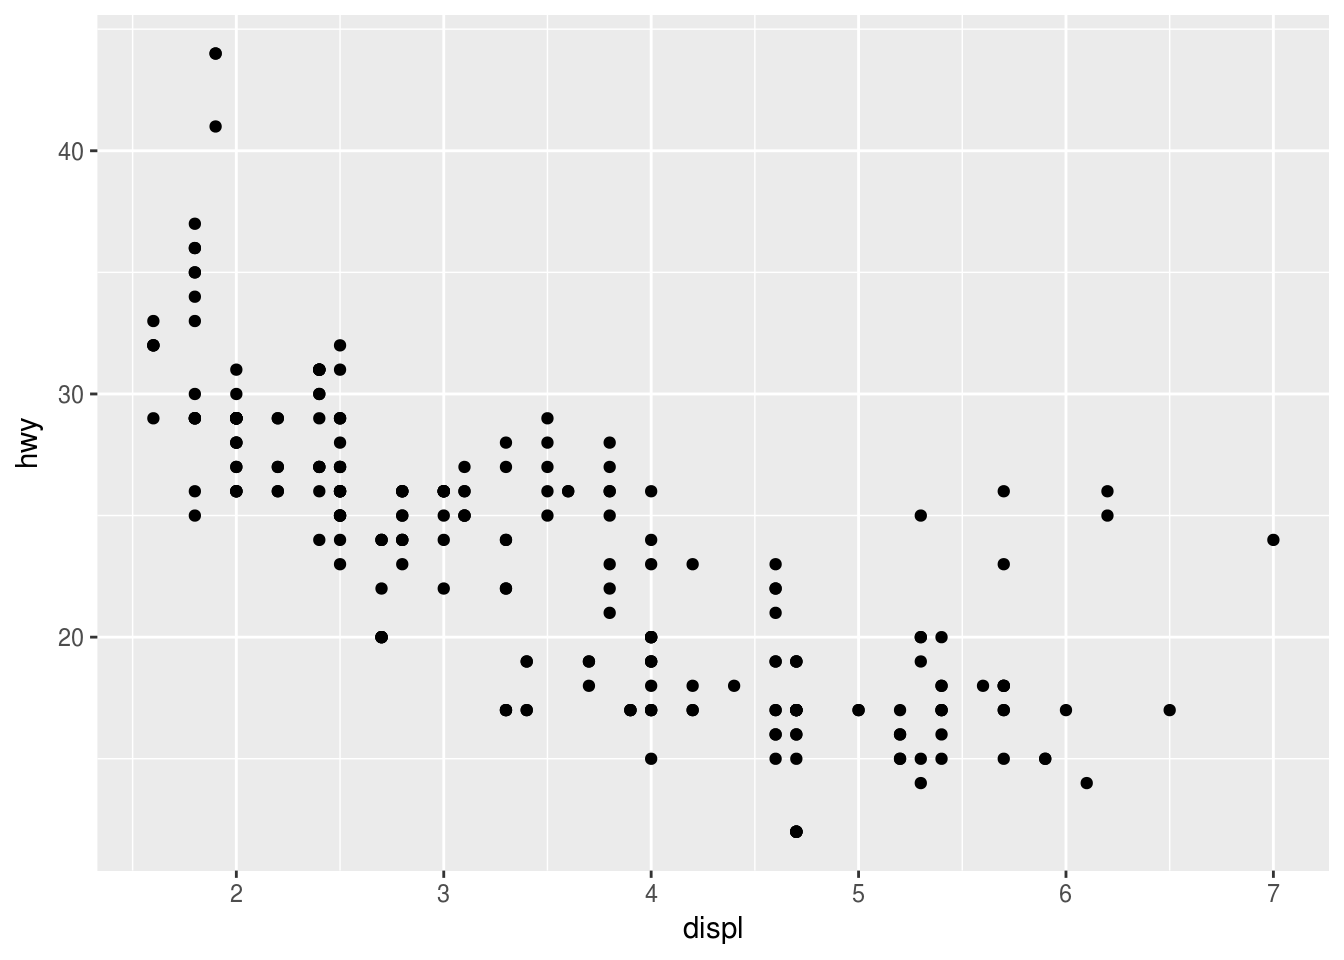
\includegraphics{ScPoEconometrics_files/figure-latex/unnamed-chunk-112-1} \end{center}

Now that doesn't seem a particularly \emph{good} way to summarize the
relationship. Clearly, a \emph{better} line would be not be flat, but
have a \emph{slope}, i.e.~go upwards:

\begin{center}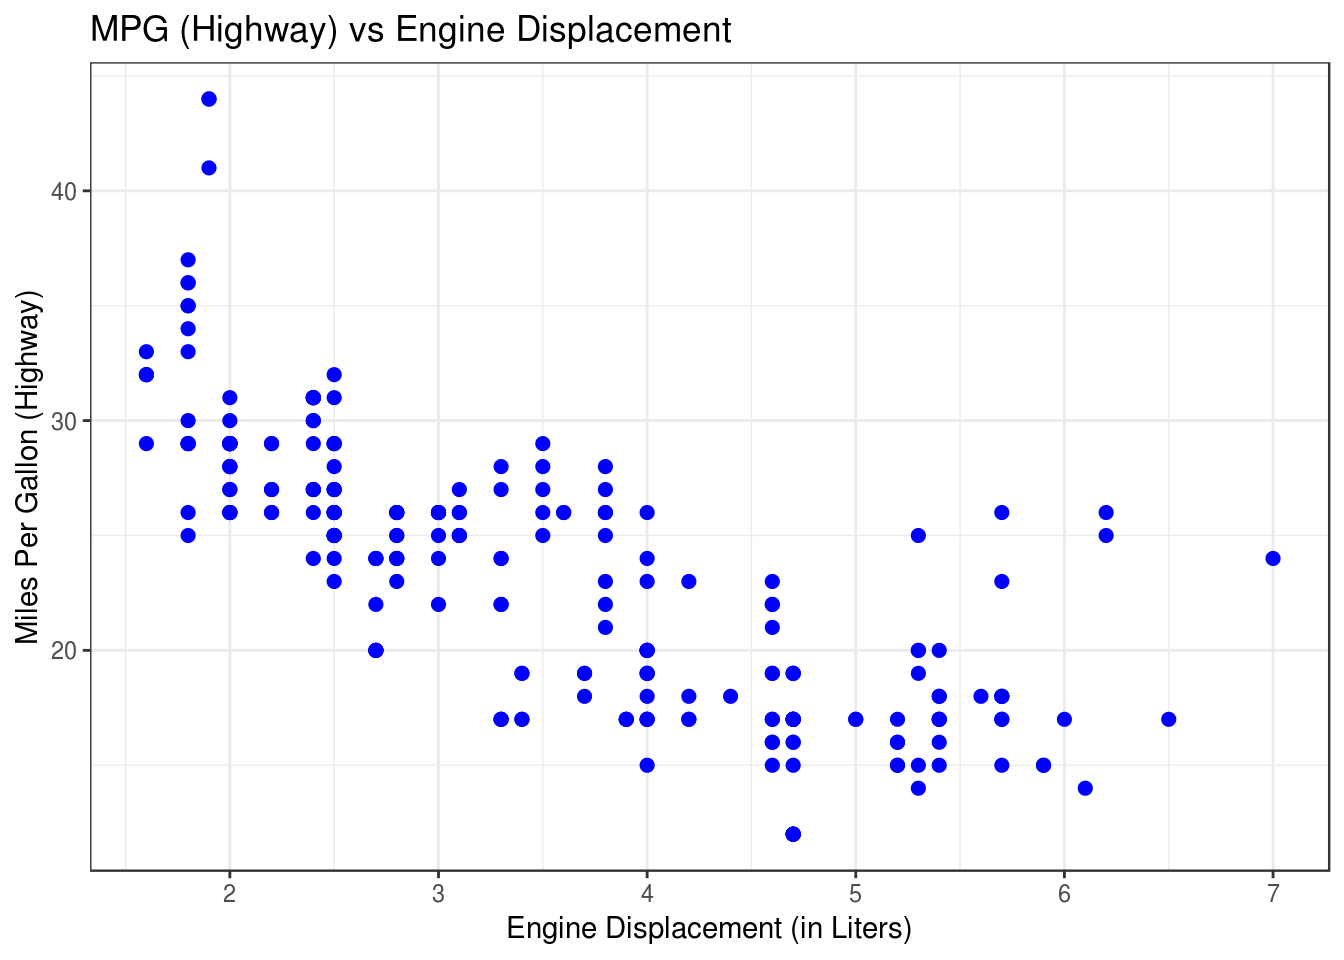
\includegraphics{ScPoEconometrics_files/figure-latex/unnamed-chunk-113-1} \end{center}

That is slightly better. However, the line seems at too high a level -
the point at which it crosses the y-axis is called the \emph{intercept};
and it's too high. We just learned how to represent a \emph{line},
i.e.~with two numbers called \emph{intercept} and \emph{slope}. Let's
write down a simple formula which represents a line where some outcome
\(z\) is related to a variable \(x\):

\begin{equation}
z = b_0 + b_1 x \label{eq:bline}
\end{equation}

Here \(b_0\) represents the value of the intercept (i.e. \(z\) when
\(x=0\)), and \(b_1\) is the value of the slope. The question for us is
now: How to choose the number \(b_0\) and \(b_1\) such that the result
is the \textbf{good} line?

\subsection{Choosing the Best Line}\label{choosing-the-best-line}

In order to be able to reason about good or bad line, we need to denote
the \emph{output} of equation \eqref{eq:bline}. We call the value
\(\hat{y}_i\) the \emph{predicted value} for obseration \(i\), after
having chosen some particular values \(b_0\) and \(b_1\):

\begin{equation}
\hat{y}_i = b_0 + b_1 x_i \label{eq:abline-pred}
\end{equation}

In general it is likely that we won't be able to choose \(b_0\) and
\(b_1\) in such as way as to provide a perfect prediction, i.e.~one
where \(\hat{y}_i = y_i\) for all \(i\). That is, we expect to make an
\emph{error} in our prediction \(\hat{y}_i\), so let's denote this value
\(e_i\). If we acknowlegdge that we will make errors, let's at least
make them as small as possible! Exactly this is going to be our task
now.

Suppose we have the following set of 9 observations on \texttt{x} and
\texttt{y}, and we put the \emph{best} straight line into it, that we
can think of. It would look like this:

\begin{figure}

{\centering 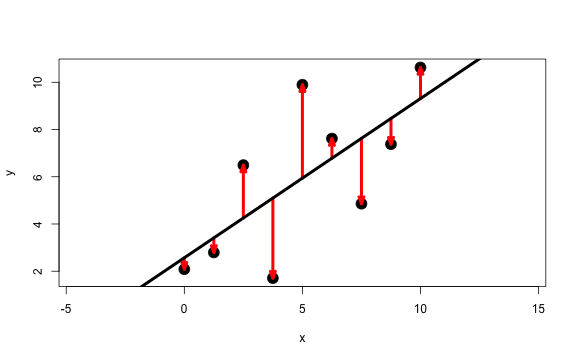
\includegraphics{ScPoEconometrics_files/figure-latex/line-arrows-1} 

}

\caption{The best line and its errors}\label{fig:line-arrows}
\end{figure}

Here, the red arrows indicate the \textbf{distance} between the
prediction (i.e.~the black line) to each data point, in other words,
each arrow is a particular \(e_i\). An upward pointing arrow indicates a
positive value of a particular \(e_i\), and vice versa for downward
pointing arrows. The erros are also called \emph{residuals}, which comes
from the way can write the equation for this relationship between two
particular values \((y_i,x_i)\) belonging to observation \(i\):

\begin{equation}
y_i = b_0 + b_1 x_i + e_i \label{eq:abline}
\end{equation}

You realize of course that \(\hat{y}_i = y_i - e_i\), which just means
that our prediction is the observed value \(y_i\) minus any error
\(e_i\) we make. In other words, \(e_i\) is what is left to be explained
on top of the line \(b_0 + b_1 x_i\), hence, it's a residual to explain
\(y_i\). Here are \(y,\hat{y}\) and the resulting \(e\) which are
plotted in figure \ref{fig:line-arrows}:

\begin{tabular}{c|c|c|c}
\hline
x & y & y\_hat & error\\
\hline
0.00 & 2.09 & 2.57 & -0.48\\
\hline
1.25 & 2.79 & 3.41 & -0.62\\
\hline
2.50 & 6.49 & 4.25 & 2.24\\
\hline
3.75 & 1.71 & 5.10 & -3.39\\
\hline
5.00 & 9.89 & 5.94 & 3.95\\
\hline
6.25 & 7.62 & 6.78 & 0.83\\
\hline
7.50 & 4.86 & 7.63 & -2.77\\
\hline
8.75 & 7.38 & 8.47 & -1.09\\
\hline
10.00 & 10.63 & 9.31 & 1.32\\
\hline
\end{tabular}

If our line was a \textbf{perfect fit} to the data, all \(e_i = 0\), and
the column \texttt{error} would display \texttt{0} for each row - there
would be no errors at all. (All points in figure \ref{fig:line-arrows}
would perfectly line up on a straight line).

Now, back to our claim that this particular line is the \emph{best}
line. What exactly characterizes this best line? We now come back to
what we said above - \emph{how to make the errors as small as possible}?
Keeping in mind that each residual \(e_i\) is \(y_i - \hat{y}_i\), we
have the following minization problem to solve:

\begin{align}
e_i & = y_i - \hat{y}_i = y_i - \underbrace{\left(b_0 + b_1 x_i\right)}_\text{prediction}\\
e_1^2 + \dots + e_N^2 &= \sum_{i=1}^N e_i^2 \equiv \text{SSR}(b_0,b_1) \\
(b_0,b_1) &= \arg \min_{\text{int},\text{slope}} \sum_{i=1}^N \left[y_i - \left(\text{int} + \text{slope } x_i\right)\right]^2 \label{eq:ols-min}
\end{align}

\begin{warning}
The best line chooses \(b_0\) and \(b_1\) so as to minimize the sum of
\textbf{squared residuals} (SSR).
\end{warning}

 Wait a moment, why \emph{squared} residuals? This is easy to
understand: suppose that instead, we wanted to just make the \emph{sum}
of the arrows in figure \ref{fig:line-arrows} as small as possible (that
is, no squares). Choosing our line to make this number small would not
give a particularly good representation of the data -- given that errors
of opposite sign and equal magnitude offset, we could have very long
arrows (but of opposite signs), and a poor resulting line. Squaring each
error avoids this (because now negative errors get positive values!)

\begin{figure}

{\centering 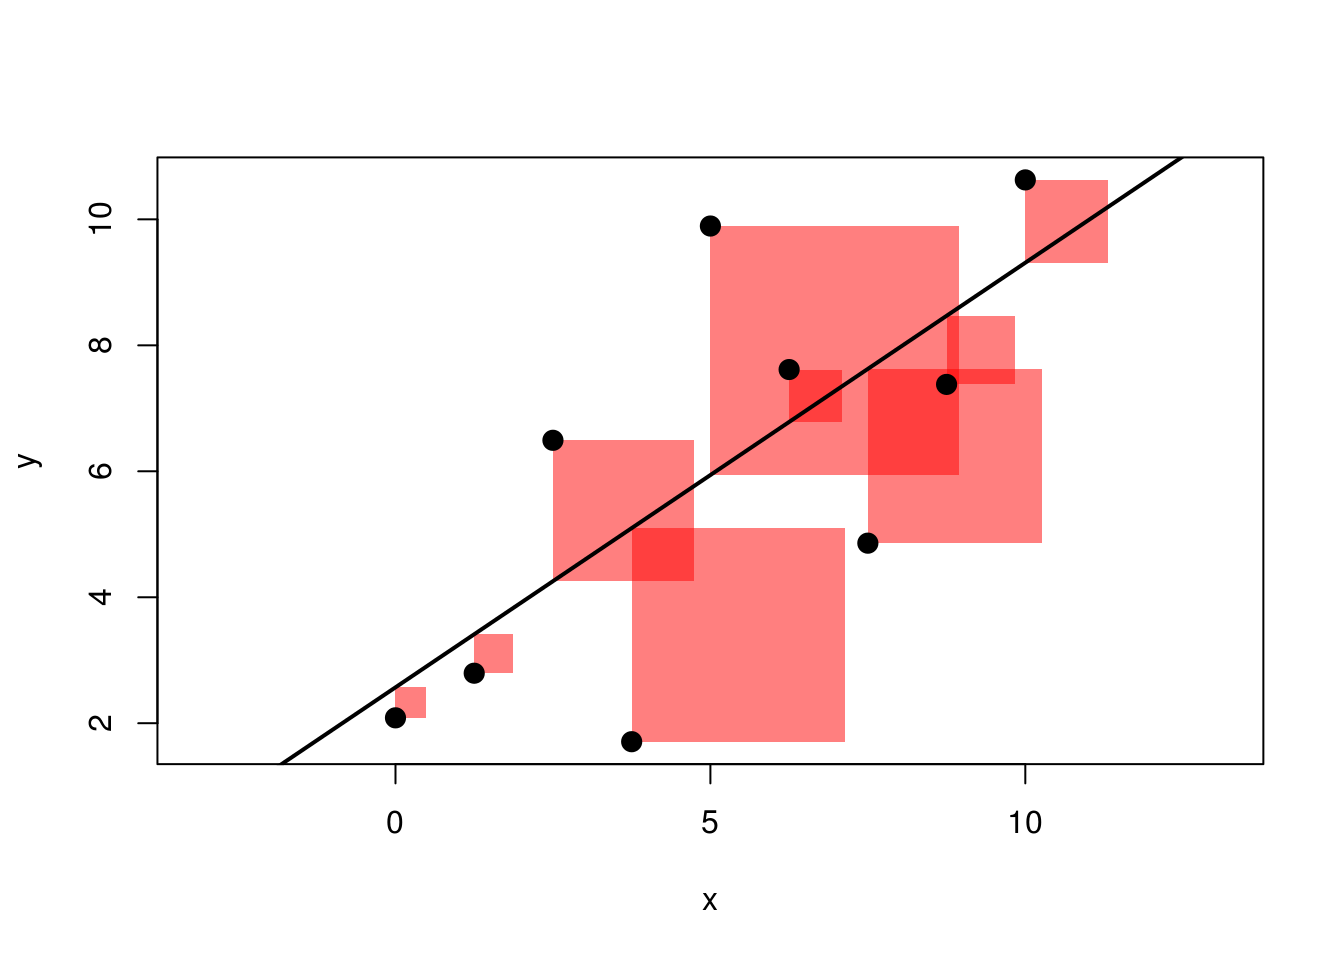
\includegraphics{ScPoEconometrics_files/figure-latex/line-squares-1} 

}

\caption{The best line and its SQUARED errors}\label{fig:line-squares}
\end{figure}

We illustrate this in figure \ref{fig:line-squares}. This is the same
data as in figure \ref{fig:line-arrows}, but instead of arrows of length
\(e_i\) for each observation \(i\), now we draw a square with side
\(e_i\), i.e.~an area of \(e_i^2\). We have two apps for you at this
point, one where you have to try and find the best line by choosing
\(b_0\) and \(b_1\), only focusing on the sum of errors (and not their
square), and a second one focusing on squared errors:

\begin{Shaded}
\begin{Highlighting}[]
\KeywordTok{library}\NormalTok{(ScPoEconometrics)}
\KeywordTok{launchApp}\NormalTok{(}\StringTok{"reg_simple_arrows"}\NormalTok{)}
\KeywordTok{launchApp}\NormalTok{(}\StringTok{"reg_simple"}\NormalTok{) }\CommentTok{# with squared errors}
\KeywordTok{launchApp}\NormalTok{(}\StringTok{"SSR_cone"}\NormalTok{) }\CommentTok{# visualize the minimzation problem from above!}
\end{Highlighting}
\end{Shaded}

Most of our \texttt{apps} have an associated \texttt{about} document,
which gives extra information and explanations. After you have looked at
all three apps, we invite you thus to have a look at the associated
explainers by typing

\begin{Shaded}
\begin{Highlighting}[]
\KeywordTok{aboutApp}\NormalTok{(}\StringTok{"reg_simple_arrows"}\NormalTok{)}
\KeywordTok{aboutApp}\NormalTok{(}\StringTok{"reg_simple"}\NormalTok{) }
\KeywordTok{aboutApp}\NormalTok{(}\StringTok{"SSR_cone"}\NormalTok{) }
\end{Highlighting}
\end{Shaded}

\section{Ordinary Least Squares (OLS) Estimator}\label{OLS}

The method to compute (or \emph{estimate}) \(b_0\) and \(b_1\) we
illustrated above is called \emph{Ordinary Least Squares}, or OLS.
\(b_0\) and \(b_1\) are therefore also often called the \emph{OLS
coefficients}. By solving problem \eqref{eq:ols-min} one can derive an
explicit formula for them:

\begin{equation}
b_1 = \frac{cov(x,y)}{var(x)},  \label{eq:beta1hat}
\end{equation}

i.e.~the estimate of the slope coefficient is the covariance between
\(x\) and \(y\) divided by the variance of \(x\), both computed from our
sample of data. With \(b_1\) in hand, we can get the estimate for the
intercept as

\begin{equation}
b_0 = \bar{y} - b_1 \bar{x}.  \label{eq:beta0hat}
\end{equation}

where \(\bar{z}\) denotes the sample mean of variable \(z\). The
interpretation of the OLS slope coefficient \(b_1\) is as follows. Given
a line as in \(y = b_0 + b_1 x\),

\begin{itemize}
\tightlist
\item
  \(b_1 = \frac{d y}{d x}\) measures the change in \(y\) resulting from
  a one unit change in \(x\)
\item
  For example, if \(y\) is wage and \(x\) is years of education, \(b_1\)
  would measure the effect of an additional year of education on wages.
\end{itemize}

There is an alternative representation for the OLS slope coefficient
which relates to the \emph{correlation coefficient} \(r\). Remember from
section \ref{summarize-two} that \(r = \frac{cov(x,y)}{s_x s_y}\), where
\(s_z\) is the standard deviation of variable \(z\). With this in hand,
we can derive the OLS slope coefficient as

\begin{align}
b_1 &= \frac{cov(x,y)}{var(x)}\\
    &= \frac{cov(x,y)}{s_x s_x} \\
    &= r\frac{s_y}{s_x} \label{eq:beta1-r}
\end{align}

In other words, the slope coefficient is equal to the correlation
coefficient \(r\) times the ratio of standard deviations of \(y\) and
\(x\).

\subsection{Linear Regression without
Regressor}\label{linear-regression-without-regressor}

There are several important special cases for the linear regression
introduced above. Let's start with the most obvious one: What is the
meaning of running a regression \emph{without any regressor},
i.e.~without a \(x\)? Our line becomes very simple. Instead of
\eqref{eq:bline}, we get

\begin{equation}
y = b_0. \label{eq:b0line}
\end{equation}

This means that our minization problem in \eqref{eq:ols-min} \emph{also}
becomes very simple: We only have to choose \(b_0\)! We have

\[
b_0 = \arg\min_{\text{int}} \sum_{i=1}^N \left[y_i - \text{int}\right]^2,
\] which is a quadratic equation with a unique optimum such that \[
b_0 = \frac{1}{N} \sum_{i=1}^N y_i = \overline{y}.
\]

\begin{tip}
Least Squares \textbf{without regressor} \(x\) estimates the sample mean
of the outcome variable \(y\), i.e.~it produces \(\overline{y}\).
\end{tip}

\subsection{Regression without an
Intercept}\label{regression-without-an-intercept}

We follow the same logic here, just that we miss another bit from our
initial equation and the minimisation problem in \eqref{eq:ols-min} now
becomes:

\begin{align}
b_1 &= \arg\min_{\text{slope}} \sum_{i=1}^N \left[y_i - \text{slope } x_i \right]^2\\
\mapsto b_1 &= \frac{\frac{1}{N}\sum_{i=1}^N x_i y_i}{\frac{1}{N}\sum_{i=1}^N x_i^2} = \frac{\bar{x} \bar{y}}{\overline{x^2}} \label{eq:b1line}
\end{align}

\begin{tip}
Least Squares \textbf{without intercept} (i.e.~with \(b_0=0\)) is a line
that passes through the origin.
\end{tip}

In this case we only get to choose the slope \(b_1\) of this anchored
line.\footnote{This slope is related to the angle between vectors
  \(\mathbf{a} = (\overline{x},\overline{y})\), and
  \(\mathbf{b} = (\overline{x},0)\). Hence, it's related to the
  \href{https://en.wikipedia.org/wiki/Scalar_projection}{scalar
  projection} of \(\mathbf{a}\) on \(\mathbf{b}\).} You should now try
out both of those restrictions on our linear model by spending some time
with

\begin{Shaded}
\begin{Highlighting}[]
\KeywordTok{launchApp}\NormalTok{(}\StringTok{"reg_constrained"}\NormalTok{)}
\end{Highlighting}
\end{Shaded}

\subsection{Centering A Regression}\label{centering-a-regression}

By \emph{centering} or \emph{demeaning} a regression, we mean to
substract from both \(y\) and \(x\) their respective averages to obtain
\(\tilde{y}_i = y_i - \bar{y}\) and \(\tilde{x}_i = x_i - \bar{x}\). We
then run a regression \emph{without intercept} as above. That is, we use
\(\tilde{x}_i,\tilde{y}_i\) instead of \(x_i,y_i\) in \eqref{eq:b1line} to
obtain our slope estimate \(b_1\):

\begin{align}
b_1 &= \frac{\frac{1}{N}\sum_{i=1}^N \tilde{x}_i \tilde{y}_i}{\frac{1}{N}\sum_{i=1}^N \tilde{x}_i^2}\\
    &= \frac{\frac{1}{N}\sum_{i=1}^N (x_i - \bar{x}) (y_i - \bar{y})}{\frac{1}{N}\sum_{i=1}^N (x_i - \bar{x})^2} \\
    &= \frac{cov(x,y)}{var(x)}
    \label{eq:bline-centered}
\end{align}

This last expression is \emph{identical} to the one in
\eqref{eq:beta1hat}! It's the standard OLS estimate for the slope
coefficient. We note the following:

\begin{tip}
Adding a constant to a regression produces the same result as centering
all variables and estimating without intercept. So, unless all variables
are centered, \textbf{always} include an intercept in the regression.
\end{tip}

 To get a better feel for what is going on here, you can try this out
now by yourself by typing:

\begin{Shaded}
\begin{Highlighting}[]
\KeywordTok{launchApp}\NormalTok{(}\StringTok{"demeaned_reg"}\NormalTok{)}
\end{Highlighting}
\end{Shaded}

\subsection{Standardizing A Regression}\label{reg-standard}

\emph{Standardizing} a variable \(z\) means to demean as above, but in
addition to divide the demeaned value by its own standard deviation.
Similarly to what we did above for \emph{centering}, we define
transformed variables \(\breve{y}_i = \frac{y_i-\bar{y}}{\sigma_y}\) and
\(\breve{x}_i = \frac{x_i-\bar{x}}{\sigma_x}\) where \(\sigma_z\) is the
standard deviation of variable \(z\). From here on, you should by now be
used to what comes next! As above, we use \(\breve{x}_i,\breve{y}_i\)
instead of \(x_i,y_i\) in \eqref{eq:b1line} to this time obtain:

\begin{align}
b_1 &= \frac{\frac{1}{N}\sum_{i=1}^N \breve{x}_i \breve{y}_i}{\frac{1}{N}\sum_{i=1}^N \breve{x}_i^2}\\
    &= \frac{\frac{1}{N}\sum_{i=1}^N \frac{x_i - \bar{x}}{\sigma_x} \frac{y_i - \bar{y}}{\sigma_y}}{\frac{1}{N}\sum_{i=1}^N \left(\frac{x_i - \bar{x}}{\sigma_x}\right)^2} \\
    &= \frac{Cov(x,y)}{\sigma_x \sigma_y} \\
    &= Corr(x,y)  \label{eq:bline-standardized}
\end{align}

\begin{tip}
After we standardize both \(y\) and \(x\), the slope coefficient \(b_1\)
in the regression without intercept is equal to the \textbf{correlation
coefficient}.
\end{tip}

 And also for this case we have a practical application for you. Just
type this and play around with the app for a little while!

\begin{Shaded}
\begin{Highlighting}[]
\KeywordTok{launchApp}\NormalTok{(}\StringTok{"reg_standardized"}\NormalTok{)}
\end{Highlighting}
\end{Shaded}

\section{Predictions and Residuals}\label{pred-resids}

Now we want to ask how our residuals \(e_i\) relate to the prediction
\(\hat{y_i}\). Let us first think about the average of all predictions
\(\hat{y_i}\), i.e.~the number \(\frac{1}{N} \sum_{i=1}^N \hat{y_i}\).
Let's just take \eqref{eq:abline-pred} and plug this into this average, so
that we get

\begin{align}
\frac{1}{N} \sum_{i=1}^N \hat{y_i} &= \frac{1}{N} \sum_{i=1}^N b_0 + b_1 x_i \\
&= b_0 + b_1  \frac{1}{N} \sum_{i=1}^N x_i \\
&= b_0 + b_1  \bar{x} \\
\end{align}

But that last line is just equal to the formula for the OLS intercept
\eqref{eq:beta0hat}, \(b_0 = \bar{y} - b_1 \bar{x}\)! That means of course
that

\[
\frac{1}{N} \sum_{i=1}^N \hat{y_i}  = b_0 + b_1  \bar{x} = \bar{y}
\] in other words:

\begin{tip}
The average of our predictions \(\hat{y_i}\) is identically equal to the
mean of the outcome \(y\). This implies that the average of the
residuals is equal to zero.
\end{tip}

 Related to this result, we can show that the prediction \(\hat{y}\) and
the residuals are \emph{uncorrelated}, something that is often called
\textbf{orthogonality} between \(\hat{y}_i\) and \(e_i\). We would write
this as

\begin{align}
Cov(\hat{y},e) &=\frac{1}{N} \sum_{i=1}^N (\hat{y}_i-\bar{y})(e_i-\bar{e}) =   \frac{1}{N} \sum_{i=1}^N (\hat{y}_i-\bar{y})e_i \\
&=  \frac{1}{N} \sum_{i=1}^N \hat{y}_i e_i-\bar{y} \frac{1}{N} \sum_{i=1}^N e_i = 0
\end{align}

It's useful to bring back the sample data which generate figure
\ref{fig:line-arrows} at this point in order to verify these claims:

\begin{verbatim}
#OUT>       y y_hat error
#OUT> 1  2.09  2.57 -0.48
#OUT> 2  2.79  3.41 -0.62
#OUT> 3  6.49  4.25  2.24
#OUT> 4  1.71  5.10 -3.39
#OUT> 5  9.89  5.94  3.95
#OUT> 6  7.62  6.78  0.83
#OUT> 7  4.86  7.63 -2.77
#OUT> 8  7.38  8.47 -1.09
#OUT> 9 10.63  9.31  1.32
\end{verbatim}

Let's check that these claims are true in this sample of data. We want
that

\begin{enumerate}
\def\labelenumi{\arabic{enumi}.}
\tightlist
\item
  The average of \(\hat{y}_i\) to be the same as the mean of \(y\)
\item
  The average of the errors should be zero.
\item
  Prediction and errors should be uncorrelated.
\end{enumerate}

\begin{Shaded}
\begin{Highlighting}[]
\CommentTok{# 1.}
\KeywordTok{all.equal}\NormalTok{(}\KeywordTok{mean}\NormalTok{(ss}\OperatorTok{$}\NormalTok{error), }\DecValTok{0}\NormalTok{)}
\end{Highlighting}
\end{Shaded}

\begin{verbatim}
#OUT> [1] TRUE
\end{verbatim}

\begin{Shaded}
\begin{Highlighting}[]
\CommentTok{# 2.}
\KeywordTok{all.equal}\NormalTok{(}\KeywordTok{mean}\NormalTok{(ss}\OperatorTok{$}\NormalTok{y_hat), }\KeywordTok{mean}\NormalTok{(ss}\OperatorTok{$}\NormalTok{y))}
\end{Highlighting}
\end{Shaded}

\begin{verbatim}
#OUT> [1] TRUE
\end{verbatim}

\begin{Shaded}
\begin{Highlighting}[]
\CommentTok{# 3.}
\KeywordTok{all.equal}\NormalTok{(}\KeywordTok{cov}\NormalTok{(ss}\OperatorTok{$}\NormalTok{error,ss}\OperatorTok{$}\NormalTok{y_hat), }\DecValTok{0}\NormalTok{)}
\end{Highlighting}
\end{Shaded}

\begin{verbatim}
#OUT> [1] TRUE
\end{verbatim}

So indeed we can confirm this result with our test dataset. Great!

\section{Correlation, Covariance and
Linearity}\label{correlation-covariance-and-linearity}

It is important to keep in mind that Correlation and Covariance relate
to a \emph{linear} relationship between \texttt{x} and \texttt{y}. Given
how the regression line is estimated by OLS (see just above), you can
see that the regression line inherits this property from the Covariance.
A famous exercise by Francis Anscombe (1973) illustrates this by
constructing 4 different datasets which all have identical
\textbf{linear} statistics: mean, variance, correlation and regression
line \emph{are identical}. However, the usefulness of the statistics to
describe the relationship in the data is not clear.

\begin{center}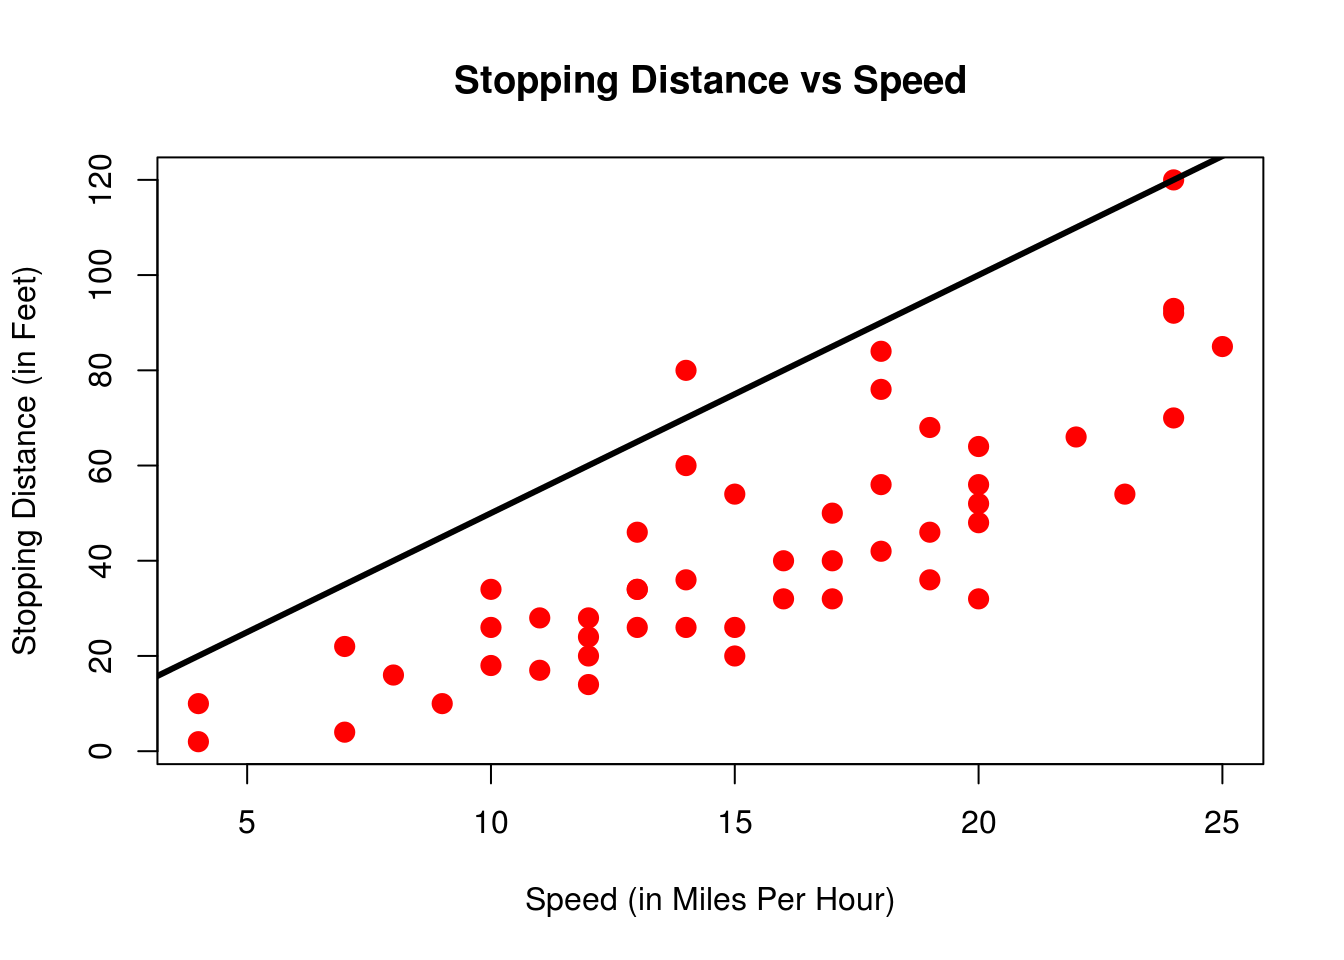
\includegraphics{ScPoEconometrics_files/figure-latex/unnamed-chunk-129-1} \end{center}

The important lesson from this example is the following:

\begin{warning}
Always \textbf{visually inspect} your data, and don't rely exclusively
on summary statistics like \emph{mean, variance, correlation and
regression line}. All of those assume a \textbf{linear} relationship
between the variables in your data.
\end{warning}

 The mission of Anscombe has been continued recently. As a result of
this we can have a look at the \texttt{datasauRus} package, which
pursues Anscbombe's idea through a multitude of funny data sets, all
with the same linear statistics. Don't just compute the covariance, or
you might actually end up looking at a Dinosaur! What? Type this to find
out:

\begin{Shaded}
\begin{Highlighting}[]
\KeywordTok{launchApp}\NormalTok{(}\StringTok{"datasaurus"}\NormalTok{)}
\KeywordTok{aboutApp}\NormalTok{(}\StringTok{"datasaurus"}\NormalTok{)}
\end{Highlighting}
\end{Shaded}

\subsection{Non-Linear Relationships in
Data}\label{non-linear-relationships-in-data}

Suppose our data now looks like this:

\begin{center}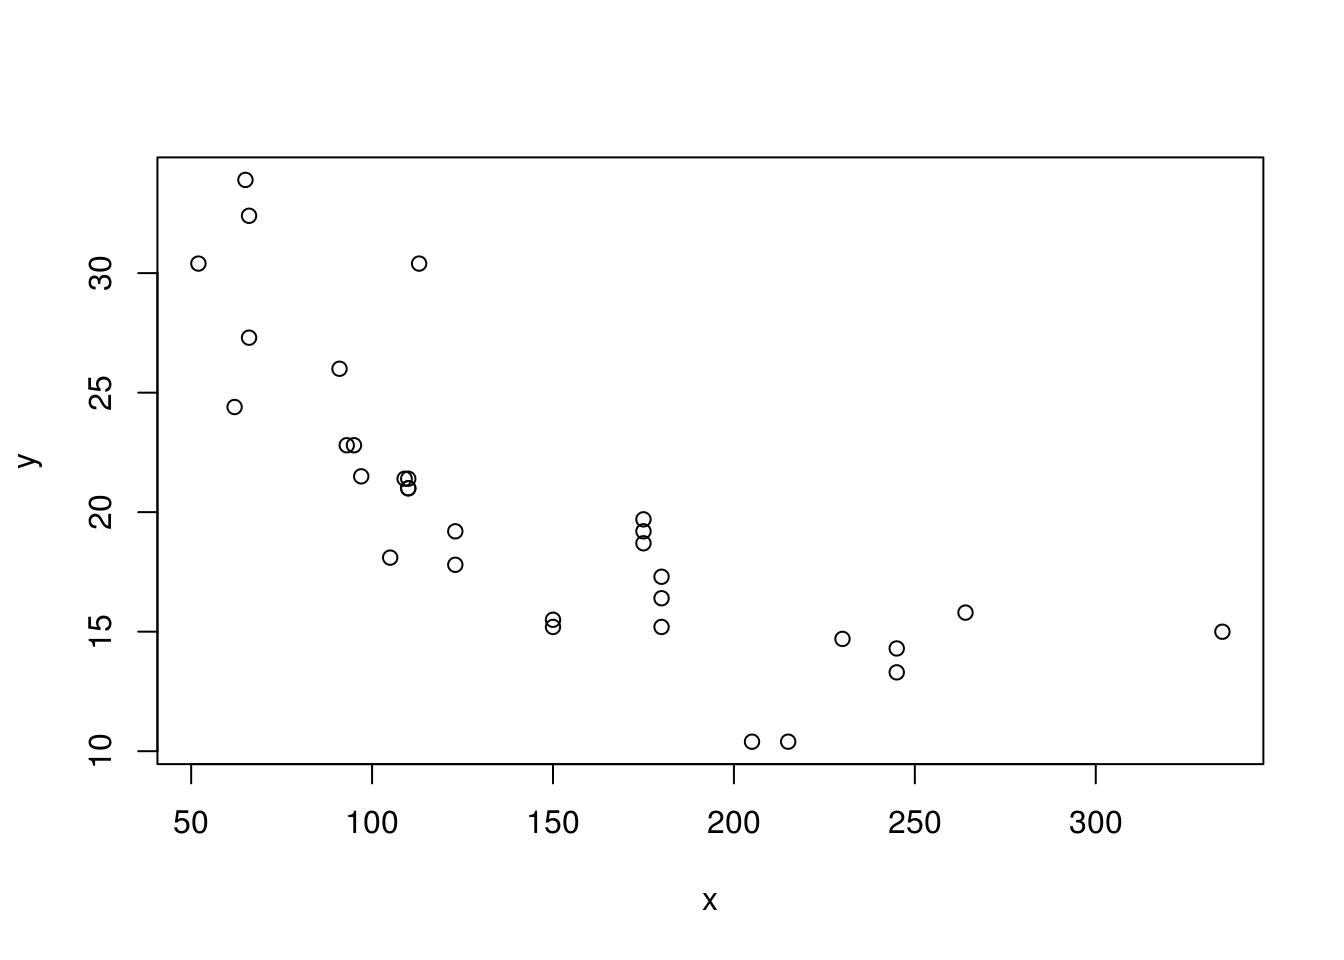
\includegraphics{ScPoEconometrics_files/figure-latex/non-line-cars-1} \end{center}

Putting our previous \emph{best line} defined in equation
\eqref{eq:abline} as \(y = b_0 + b_1 x + e\), we get something like this:

\begin{figure}

{\centering 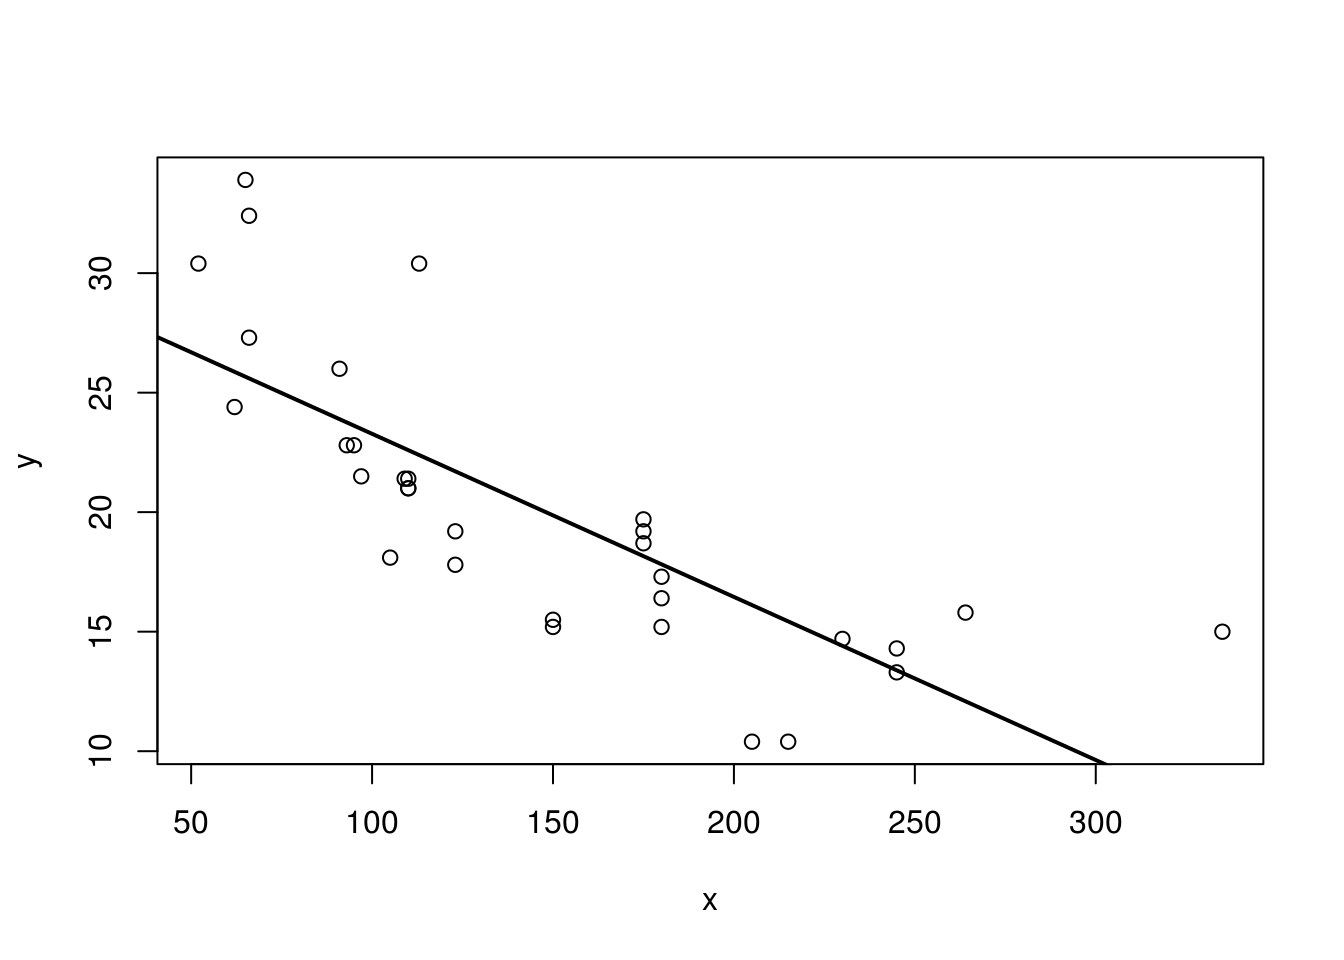
\includegraphics{ScPoEconometrics_files/figure-latex/non-line-cars-ols-1} 

}

\caption{Best line with non-linear data?}\label{fig:non-line-cars-ols}
\end{figure}

Somehow when looking at \ref{fig:non-line-cars-ols} one is not totally
convinced that the straight line is a good summary of this relationship.
For values \(x\in[50,120]\) the line seems to low, then again too high,
and it completely misses the right boundary. It's easy to address this
shortcoming by including \emph{higher order terms} of an explanatory
variable. We would modify \eqref{eq:abline} to read now

\begin{equation}
y_i = b_0 + b_1 x_i + b_2 x_i^2 + e_i \label{eq:abline2}
\end{equation}

This is a special case of \emph{multiple regression}, which we will talk
about in chapter \ref{multiple-reg}. You can see that there are
\emph{multiple} slope coefficients. For now, let's just see how this
performs:

\begin{figure}

{\centering 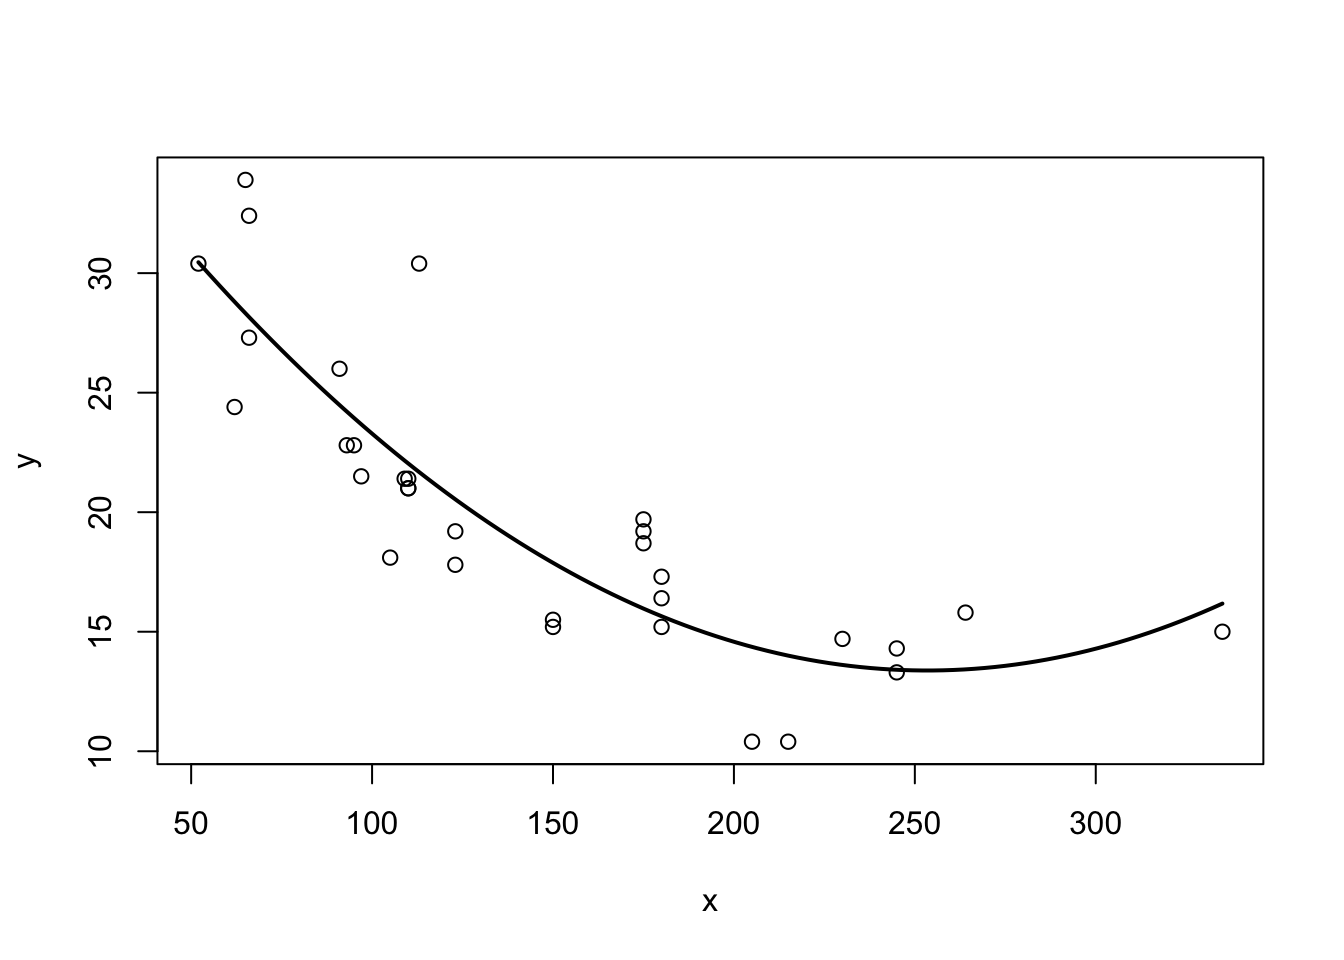
\includegraphics{ScPoEconometrics_files/figure-latex/non-line-cars-ols2-1} 

}

\caption{Better line with non-linear data!}\label{fig:non-line-cars-ols2}
\end{figure}

\section{\texorpdfstring{Analysing
\(Var(y)\)}{Analysing Var(y)}}\label{analysing-vary}

Analysis of Variance (ANOVA) refers to a method to decompose variation
in one variable as a function of several others. We can use this idea on
our outcome \(y\). Suppose we wanted to know the variance of \(y\),
keeping in mind that, by definition, \(y_i = \hat{y}_i + e_i\). We would
write

\begin{align}
Var(y) &= Var(\hat{y} + e)\\
 &= Var(\hat{y}) + Var(e) + 2 Cov(\hat{y},e)\\
 &= Var(\hat{y}) + Var(e) \label{eq:anova}
\end{align}

We have seen above in \ref{pred-resids} that the covariance between
prediction \(\hat{y}\) and error \(e\) is zero, that's why we have
\(Cov(\hat{y},e)=0\) in \eqref{eq:anova}. What this tells us in words is
that we can decompose the variance in the observed outcome \(y\) into a
part that relates to variance as \emph{explained by the model} and a
part that comes from unexplained variation. Finally, we know the
definition of \emph{variance}, and can thus write down the respective
formulae for each part:

\begin{itemize}
\tightlist
\item
  \(Var(y) = \frac{1}{N}\sum_{i=1}^N (y_i - \bar{y})^2\)
\item
  \(Var(\hat{y}) = \frac{1}{N}\sum_{i=1}^N (\hat{y_i} - \bar{y})^2\),
  because the mean of \(\hat{y}\) is \(\bar{y}\) as we know. Finally,
\item
  \(Var(e) = \frac{1}{N}\sum_{i=1}^N e_i^2\), because the mean of \(e\)
  is zero.
\end{itemize}

We can thus formulate how the total variation in outcome \(y\) is
aportioned between model and unexplained variation:

\begin{tip}
The total variation in outcome \(y\) (often called SST, or \emph{total
sum of squares}) is equal to the sum of explained squares (SSE) plus the
sum of residuals (SSR). We have thus \textbf{SST = SSE + SSR}.
\end{tip}

\section{\texorpdfstring{Assessing the \emph{Goodness of
Fit}}{Assessing the Goodness of Fit}}\label{assessing-the-goodness-of-fit}

In our setup, there exists a convenient measure for how good a
particular statistical model fits the data. It is called \(R^2\)
(\emph{R squared}), also called the \emph{coefficient of determination}.
We make use of the just introduced decomposition of variance, and write
the formula as

\begin{equation}
R^2 = \frac{\text{variance explained}}{\text{total variance}} = \frac{SSE}{SST} = 1 - \frac{SSR}{SST}\in[0,1]  \label{eq:Rsquared}
\end{equation}

It is easy to see that a \emph{good fit} is one where the sum of
\emph{explained} squares (SSE) is large relativ to the total variation
(SST). In such a case, we observe an \(R^2\) close to one. In the
opposite case, we will see an \(R^2\) close to zero. Notice that a small
\(R^2\) does not imply that the model is useless, just that it explains
a small fraction of the observed variation.

\section{An Example: California Student Test Scores}\label{lm-example1}

Luckily for us, fitting a linear model to some data does not require us
to iteratively find the best intercept and slope manually, as you have
experienced in our \texttt{apps}. As it turns out, \texttt{R} can do
this much more precisely, and very fast!

Let's explore how to do this, using a real life dataset taken from the
\texttt{Ecdat} package which includes many economics-related dataset. In
this example, we will use the \texttt{Caschool} dataset which contains
the average test scores of 420 elementary schools in California along
with some additional information.

\subsection{Loading and exploring
Data}\label{loading-and-exploring-data}

We can explore which variables are included in the dataset using the
\texttt{names()} function:

\begin{Shaded}
\begin{Highlighting}[]
\KeywordTok{library}\NormalTok{(}\StringTok{"Ecdat"}\NormalTok{) }\CommentTok{# Load the Ecdat library}
\KeywordTok{names}\NormalTok{(Caschool) }\CommentTok{# Display the variables of the Caschool dataset}
\end{Highlighting}
\end{Shaded}

\begin{verbatim}
#OUT>  [1] "distcod"  "county"   "district" "grspan"   "enrltot"  "teachers"
#OUT>  [7] "calwpct"  "mealpct"  "computer" "testscr"  "compstu"  "expnstu" 
#OUT> [13] "str"      "avginc"   "elpct"    "readscr"  "mathscr"
\end{verbatim}

For each variable in the dataset, basic summary statistics can be
obtained by calling \texttt{summary()}

\begin{Shaded}
\begin{Highlighting}[]
\KeywordTok{summary}\NormalTok{(Caschool[, }\KeywordTok{c}\NormalTok{(}\StringTok{"testscr"}\NormalTok{, }\StringTok{"str"}\NormalTok{, }\StringTok{"avginc"}\NormalTok{)])}
\end{Highlighting}
\end{Shaded}

\begin{verbatim}
#OUT>     testscr           str            avginc      
#OUT>  Min.   :605.5   Min.   :14.00   Min.   : 5.335  
#OUT>  1st Qu.:640.0   1st Qu.:18.58   1st Qu.:10.639  
#OUT>  Median :654.5   Median :19.72   Median :13.728  
#OUT>  Mean   :654.2   Mean   :19.64   Mean   :15.317  
#OUT>  3rd Qu.:666.7   3rd Qu.:20.87   3rd Qu.:17.629  
#OUT>  Max.   :706.8   Max.   :25.80   Max.   :55.328
\end{verbatim}

\subsection{Fitting a linear model}\label{fitting-a-linear-model}

Suppose we are interested in the following linear model:

\[\text{testscr}_i = b_0 + b_1 \times \text{str}_i + e_i\] Where
\(\text{testscr}_i\) is the \emph{average test score} for a given school
\(i\) and \(\text{str}_i\) is the \emph{Student/Teacher Ratio} (i.e.~the
average number of students per teacher) in the same school \(i\). Again,
\(b_0\) and \(b_1\) are the intercept and the slope of the regression
line.

The subscript \(i\) indexes all unique elementary schools
(\(i \in \{1, 2, 3, \dots 420\}\)) and \(e_i\) is the error, or
\emph{residual}, of the regression. (Remember that our procedure for
finding the line of best fit is to minimize the \emph{sum of squared
residuals} (SSR)).

At this point you should step back and take a second to think about what
you believe the relation between a school's test scores and
student/teacher ratio will be. Do you believe that, in general, a high
student/teacher ratio will be associated with higher-than-average test
scores for the school? Do you think that the number of students per
teacher will impact results in any way?

Let's find out! As always, we will start by plotting the data to inspect
it visually:

\begin{Shaded}
\begin{Highlighting}[]
\KeywordTok{plot}\NormalTok{(}\DataTypeTok{formula =}\NormalTok{ testscr }\OperatorTok{~}\StringTok{ }\NormalTok{str,}
     \DataTypeTok{data =}\NormalTok{ Caschool,}
     \DataTypeTok{xlab =} \StringTok{"Student/Teacher Ratio"}\NormalTok{,}
     \DataTypeTok{ylab =} \StringTok{"Average Test Score"}\NormalTok{, }\DataTypeTok{pch =} \DecValTok{21}\NormalTok{, }\DataTypeTok{col =} \StringTok{'blue'}\NormalTok{)}
\end{Highlighting}
\end{Shaded}

\begin{figure}

{\centering 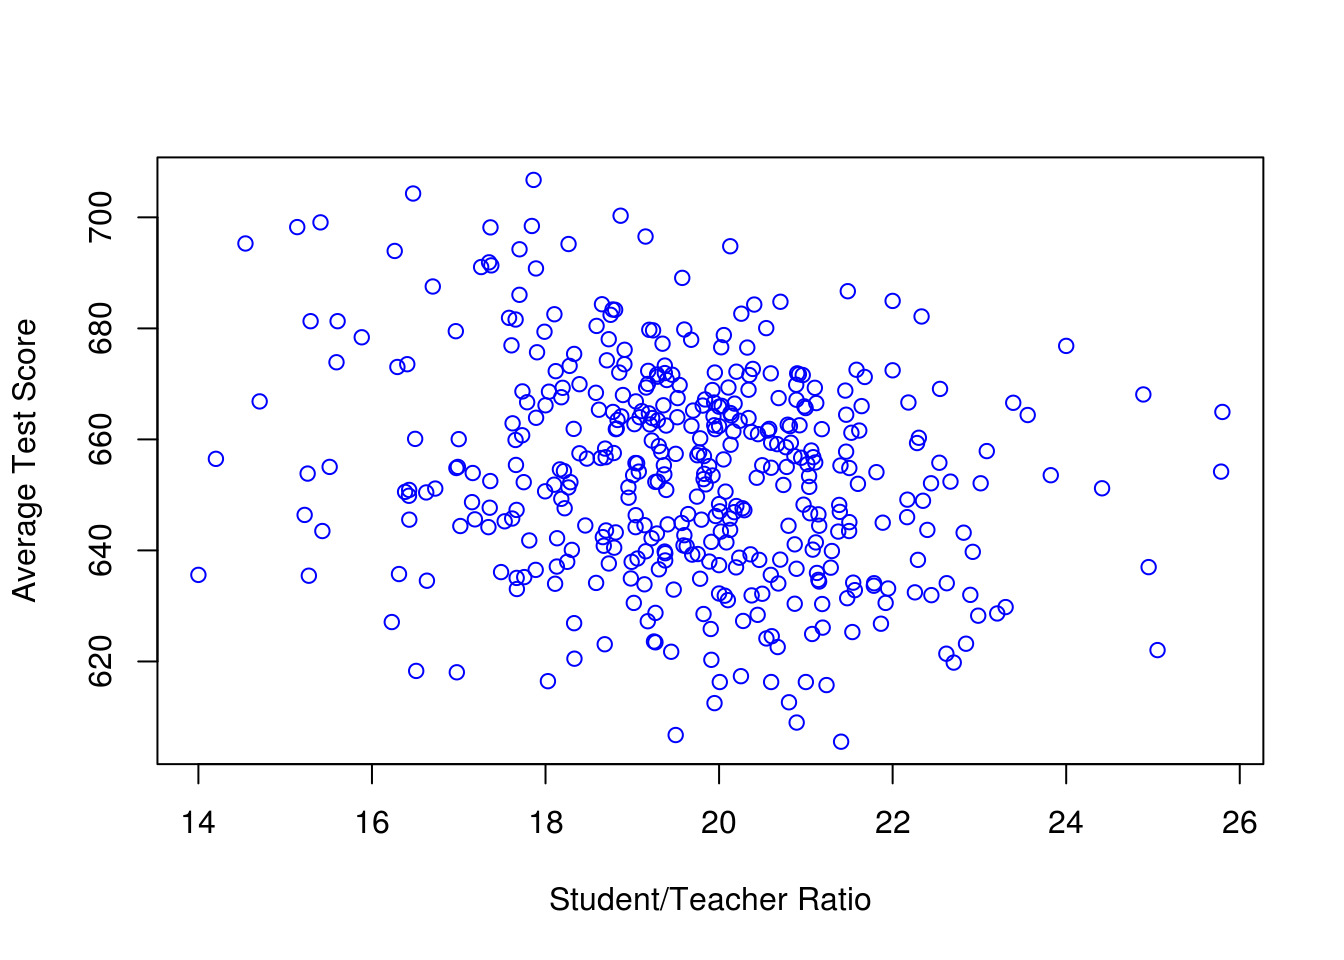
\includegraphics{ScPoEconometrics_files/figure-latex/first-reg0-1} 

}

\caption{Student Teacher Ratio vs Test Scores}\label{fig:first-reg0}
\end{figure}

Can you spot a trend in the data? According to you, what would the line
of best fit look like? Would it be upward or downward slopping? Let's
ask \texttt{R}!

\subsection{\texorpdfstring{The \texttt{lm()}
function}{The lm() function}}\label{the-lm-function}

We will use the built-in \texttt{lm()} function to estimate the
coefficients \(b_0\) and \(b_1\) using the data at hand. \texttt{lm}
stands for \emph{linear model}, which is what our representation in
\eqref{eq:abline} amounts to. This function typically only takes 2
arguments, \texttt{formula} and \texttt{data}:

\texttt{lm(formula,\ data)}

\begin{itemize}
\item
  \texttt{formula} is the description of our model which we want
  \texttt{R} to estimate for us. Its syntax is very simple:
  \texttt{Y\ \textasciitilde{}\ X} (more generally,
  \texttt{DependentVariable\ \textasciitilde{}\ Independent\ Variables}).
  You can think of the tilda operator \texttt{\textasciitilde{}} as the
  equal sign in your model equation. An intercept is included by default
  and so you do not have to ask for it in \texttt{formula}. For example,
  the simple model \(income = b_0 + b_1 \cdot age\) can be written as
  \texttt{income\ \textasciitilde{}\ age}. A \texttt{formula} can
  sometimes be written between quotation marks:
  \texttt{"X\ \textasciitilde{}\ Y"}.
\item
  \texttt{data} is simply the \texttt{data.frame} containing the
  variables in the model.
\end{itemize}

In the context of our example, the function call is therefore:

\begin{Shaded}
\begin{Highlighting}[]
\CommentTok{# assign lm() output to some object `fit_cal`}
\NormalTok{fit_cal <-}\StringTok{ }\KeywordTok{lm}\NormalTok{(}\DataTypeTok{formula =}\NormalTok{ testscr }\OperatorTok{~}\StringTok{ }\NormalTok{str, }\DataTypeTok{data =}\NormalTok{ Caschool)}

\CommentTok{# ask R for the regression summary}
\KeywordTok{summary}\NormalTok{(fit_cal) }
\end{Highlighting}
\end{Shaded}

\begin{verbatim}
#OUT> 
#OUT> Call:
#OUT> lm(formula = testscr ~ str, data = Caschool)
#OUT> 
#OUT> Residuals:
#OUT>     Min      1Q  Median      3Q     Max 
#OUT> -47.727 -14.251   0.483  12.822  48.540 
#OUT> 
#OUT> Coefficients:
#OUT>             Estimate Std. Error t value Pr(>|t|)    
#OUT> (Intercept) 698.9330     9.4675  73.825  < 2e-16 ***
#OUT> str          -2.2798     0.4798  -4.751 2.78e-06 ***
#OUT> ---
#OUT> Signif. codes:  0 '***' 0.001 '**' 0.01 '*' 0.05 '.' 0.1 ' ' 1
#OUT> 
#OUT> Residual standard error: 18.58 on 418 degrees of freedom
#OUT> Multiple R-squared:  0.05124, Adjusted R-squared:  0.04897 
#OUT> F-statistic: 22.58 on 1 and 418 DF,  p-value: 2.783e-06
\end{verbatim}

As we can see, \texttt{R} returns its estimates for the Intercept and
Slope coefficients, \(b_0 =\) 698.93 and \(b_1 =\) -2.28. The estimated
relationship between a school's Student/Teacher Ratio and its average
test results is \textbf{negative}.

The output of the \texttt{summary} method for an \texttt{lm} object is
commonly called a \emph{regression table}, and you will be able to
decypher it by the end of this course. You should be able to find an
interpret the \(R^2\) though: Are we explaining a lot of the variance in
\texttt{testscr} with this simple model, or are we not?

\subsection{Plotting the regression
line}\label{plotting-the-regression-line}

We can also use our \texttt{lm} fit to draw the regression line on top
of our initial scatterplot, using the following syntax:

\begin{Shaded}
\begin{Highlighting}[]
\KeywordTok{plot}\NormalTok{(}\DataTypeTok{formula =}\NormalTok{ testscr }\OperatorTok{~}\StringTok{ }\NormalTok{str,}
     \DataTypeTok{data =}\NormalTok{ Caschool,}
     \DataTypeTok{xlab =} \StringTok{"Student/Teacher Ratio"}\NormalTok{,}
     \DataTypeTok{ylab =} \StringTok{"Average Test Score"}\NormalTok{, }\DataTypeTok{pch =} \DecValTok{21}\NormalTok{, }\DataTypeTok{col =} \StringTok{'blue'}\NormalTok{)}\CommentTok{# same plot as before}
\KeywordTok{abline}\NormalTok{(fit_cal, }\DataTypeTok{col =} \StringTok{'red'}\NormalTok{) }\CommentTok{# add regression line}
\end{Highlighting}
\end{Shaded}

\begin{figure}

{\centering 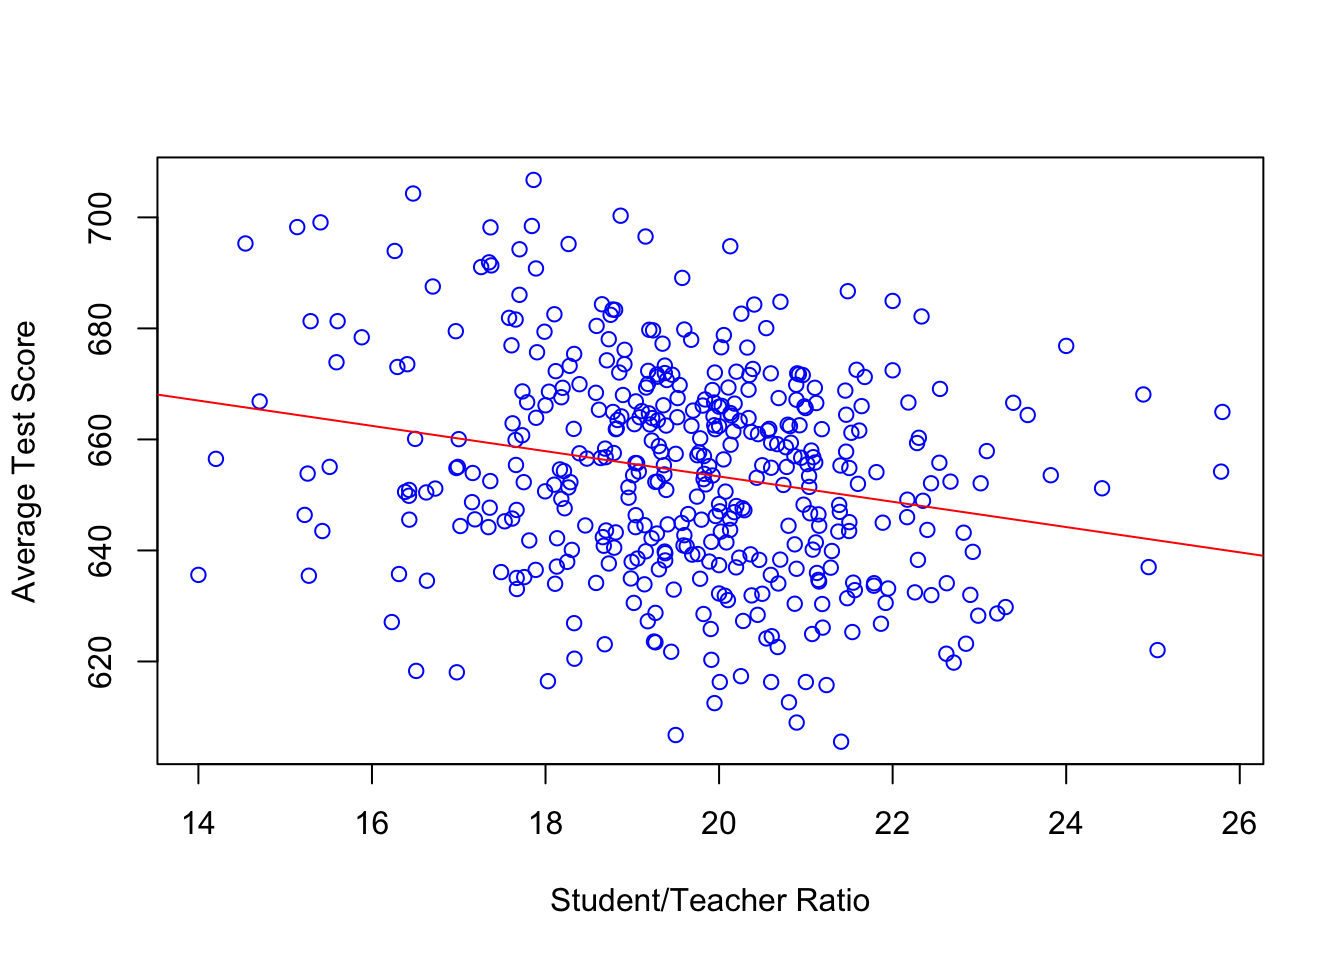
\includegraphics{ScPoEconometrics_files/figure-latex/plot-reg1-1} 

}

\caption{Test Scores with Regression Line}\label{fig:plot-reg1}
\end{figure}

As you probably expected, the best line for schools' Student/Teacher
Ratio and its average test results is downward sloping.

Just as a way of showcasing another way to make the above plot, here is
how you could use \texttt{ggplot}:

\begin{Shaded}
\begin{Highlighting}[]
\KeywordTok{library}\NormalTok{(ggplot2)}
\NormalTok{p <-}\StringTok{ }\KeywordTok{ggplot}\NormalTok{(}\DataTypeTok{mapping =} \KeywordTok{aes}\NormalTok{(}\DataTypeTok{x =}\NormalTok{ str, }\DataTypeTok{y =}\NormalTok{ testscr), }\DataTypeTok{data =}\NormalTok{ Caschool) }\CommentTok{# base plot}
\NormalTok{p <-}\StringTok{ }\NormalTok{p }\OperatorTok{+}\StringTok{ }\KeywordTok{geom_point}\NormalTok{() }\CommentTok{# add points}
\NormalTok{p <-}\StringTok{ }\NormalTok{p }\OperatorTok{+}\StringTok{ }\KeywordTok{geom_smooth}\NormalTok{(}\DataTypeTok{method =} \StringTok{"lm"}\NormalTok{, }\DataTypeTok{size=}\DecValTok{1}\NormalTok{, }\DataTypeTok{color=}\StringTok{"red"}\NormalTok{) }\CommentTok{# add regression line}
\NormalTok{p <-}\StringTok{ }\NormalTok{p }\OperatorTok{+}\StringTok{ }\KeywordTok{scale_y_continuous}\NormalTok{(}\DataTypeTok{name =} \StringTok{"Average Test Score"}\NormalTok{) }\OperatorTok{+}\StringTok{ }
\StringTok{         }\KeywordTok{scale_x_continuous}\NormalTok{(}\DataTypeTok{name =} \StringTok{"Student/Teacher Ratio"}\NormalTok{)}
\NormalTok{p }\OperatorTok{+}\StringTok{ }\KeywordTok{theme_bw}\NormalTok{() }\OperatorTok{+}\StringTok{ }\KeywordTok{ggtitle}\NormalTok{(}\StringTok{"Testscores vs Student/Teacher Ratio"}\NormalTok{)}
\end{Highlighting}
\end{Shaded}

\begin{center}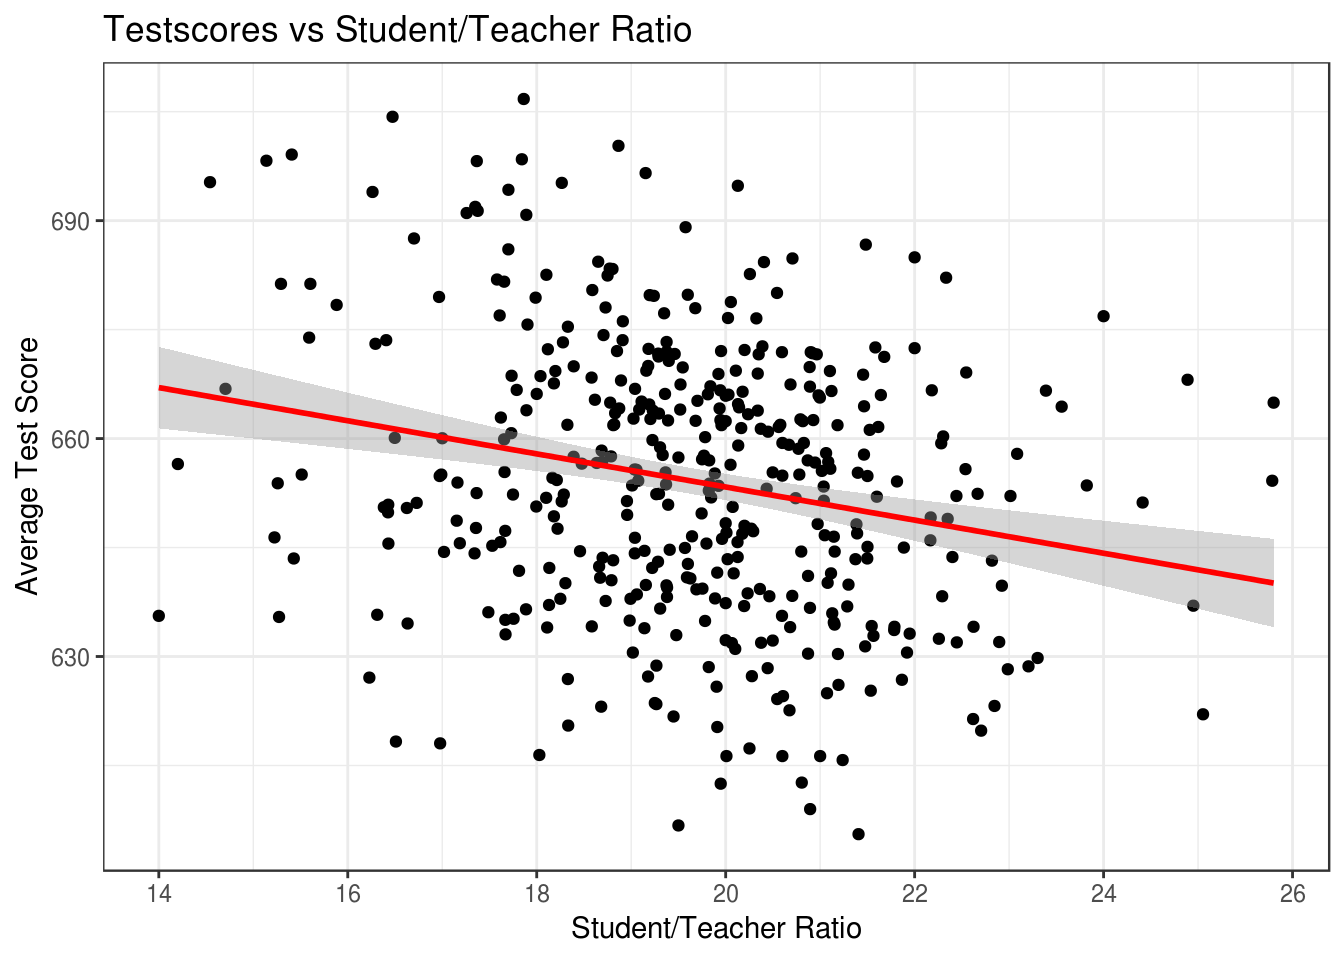
\includegraphics{ScPoEconometrics_files/figure-latex/unnamed-chunk-133-1} \end{center}

The shaded area around the red line shows the width of the 95\%
confidence interval around our estimate of the slope coefficient
\(b_1\). We will learn more about it in chapter \ref{std-errors}.

\chapter{Multiple Regression}\label{multiple-reg}

We can extend the discussion from chapter \ref{linreg} to more than one
explanatory variable. For example, suppose that instead of only \(x\) we
now had \(x_1\) and \(x_2\) in order to explain \(y\). Everything we've
learned for the single variable case applies here as well. Instead of a
regression \emph{line}, we now get a regression \emph{plane}, i.e.~an
object representable in 3 dimenions: \((x_1,x_2,y)\). As an example,
suppose we wanted to explain how many \emph{miles per gallon}
(\texttt{mpg}) a car can travel as a function of its \emph{horse power}
(\texttt{hp}) and its \emph{weight} (\texttt{wt}). In other words we
want to estimate the equation

\begin{equation}
mpg_i = b_0 + b_1 hp_i + b_2 wt_i + e_i \label{eq:abline2d}
\end{equation}

on our built-in dataset of cars (\texttt{mtcars}):

\begin{Shaded}
\begin{Highlighting}[]
\KeywordTok{subset}\NormalTok{(mtcars, }\DataTypeTok{select =} \KeywordTok{c}\NormalTok{(mpg,hp,wt))}
\end{Highlighting}
\end{Shaded}

\begin{verbatim}
#OUT>                      mpg  hp    wt
#OUT> Mazda RX4           21.0 110 2.620
#OUT> Mazda RX4 Wag       21.0 110 2.875
#OUT> Datsun 710          22.8  93 2.320
#OUT> Hornet 4 Drive      21.4 110 3.215
#OUT> Hornet Sportabout   18.7 175 3.440
#OUT> Valiant             18.1 105 3.460
#OUT> Duster 360          14.3 245 3.570
#OUT> Merc 240D           24.4  62 3.190
#OUT> Merc 230            22.8  95 3.150
#OUT> Merc 280            19.2 123 3.440
#OUT> Merc 280C           17.8 123 3.440
#OUT> Merc 450SE          16.4 180 4.070
#OUT> Merc 450SL          17.3 180 3.730
#OUT> Merc 450SLC         15.2 180 3.780
#OUT> Cadillac Fleetwood  10.4 205 5.250
#OUT> Lincoln Continental 10.4 215 5.424
#OUT> Chrysler Imperial   14.7 230 5.345
#OUT> Fiat 128            32.4  66 2.200
#OUT> Honda Civic         30.4  52 1.615
#OUT> Toyota Corolla      33.9  65 1.835
#OUT> Toyota Corona       21.5  97 2.465
#OUT> Dodge Challenger    15.5 150 3.520
#OUT> AMC Javelin         15.2 150 3.435
#OUT> Camaro Z28          13.3 245 3.840
#OUT> Pontiac Firebird    19.2 175 3.845
#OUT> Fiat X1-9           27.3  66 1.935
#OUT> Porsche 914-2       26.0  91 2.140
#OUT> Lotus Europa        30.4 113 1.513
#OUT> Ford Pantera L      15.8 264 3.170
#OUT> Ferrari Dino        19.7 175 2.770
#OUT> Maserati Bora       15.0 335 3.570
#OUT> Volvo 142E          21.4 109 2.780
\end{verbatim}

How do you think \texttt{hp} and \texttt{wt} will influence how many
miles per gallon of gasoline each of those cars can travel? In other
words, what do you expect the signs of \(b_1\) and \(b_2\) to be?

With two explanatory variables as here, it is still possible to
visualize the regression plane, so let's start with this as an answer.
The OLS regression plane through this dataset looks like in figure
\ref{fig:plane3D-reg}:

\begin{figure}

{\centering 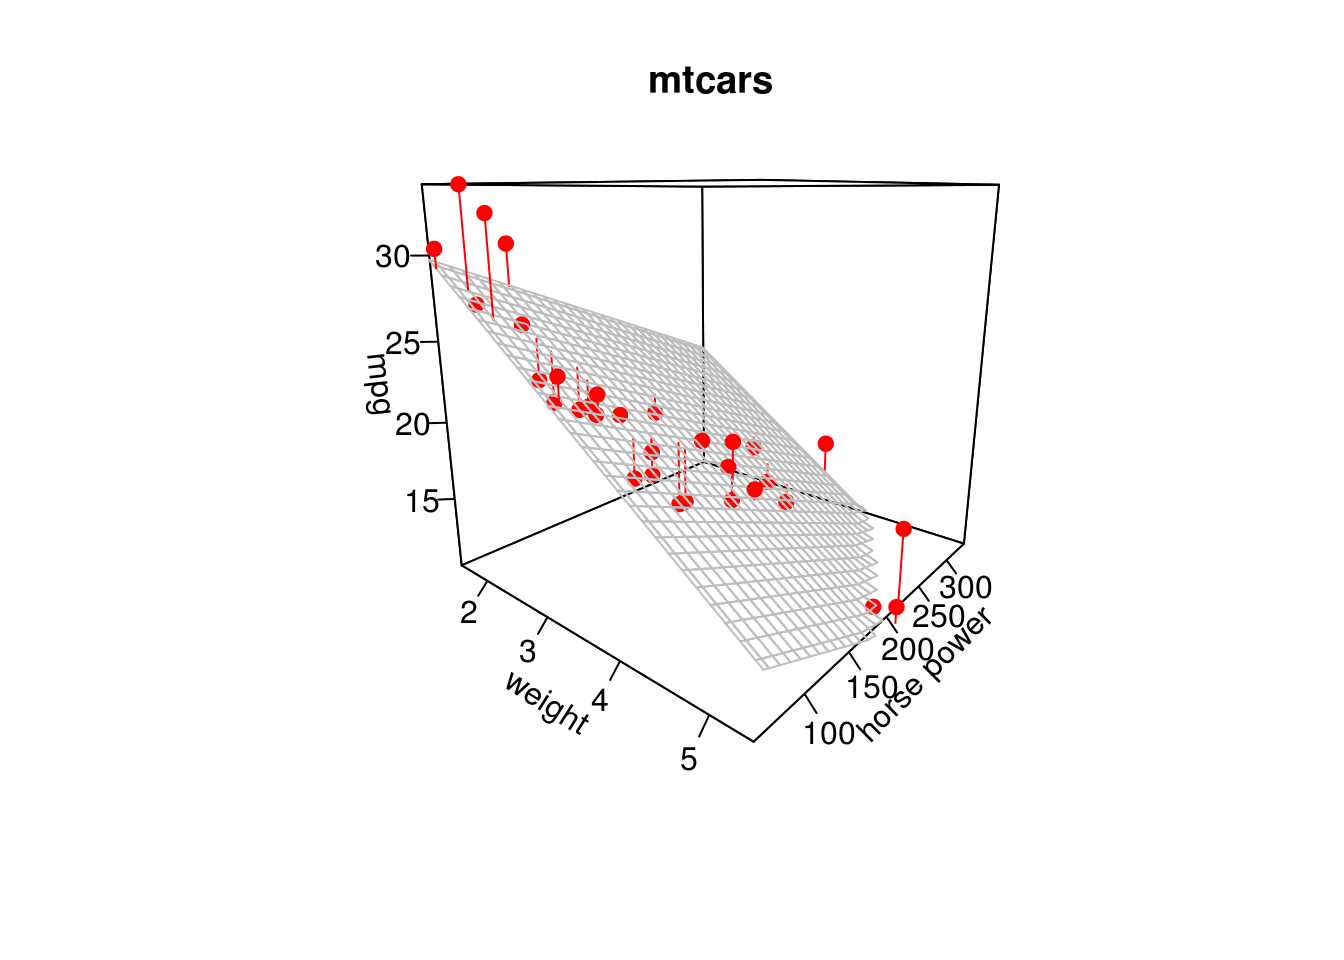
\includegraphics{ScPoEconometrics_files/figure-latex/plane3D-reg-1} 

}

\caption{Multiple Regression - a plane in 3D. The red lines indicate the residual for each observation.}\label{fig:plane3D-reg}
\end{figure}

This visualization shows a couple of things: the data are shown with red
points and the grey plane is the one resulting from OLS estimation of
equation \eqref{eq:abline2d}. You should realize that this is exactly the
same story as told in figure \ref{fig:line-arrows} - just in three
dimensions!

Furthermore, \emph{multiple} regression refers the fact that there could
be \emph{more} than two regressors. In fact, you could in principle have
\(K\) regressors, and our theory developed so far would still be valid:

\begin{align}
\hat{y}_i &= b_0 + b_1 x_{1i} +   b_2 x_{2i} + \dots + b_K x_{Ki}\\
e_i &= y_i - \hat{y}_i \label{eq:multiple-reg}
\end{align}

Just as before, the least squares method chooses numbers
\((b_0,b_1,\dots,b_K)\) to as to minimize SSR, exactly as in the
minimization problem for the one regressor case seen in
\eqref{eq:ols-min}.

\section{All Else Equal}\label{ceteris}

We can see from the above plot that cars with more horse power and
greater weight, in general travel fewer miles per gallon of combustible.
Hence, we observe a plane that is downward sloping in both the
\emph{weight} and \emph{horse power} directions. Suppose now we wanted
to know impact of \texttt{hp} on \texttt{mpg} \emph{in isolation}, so as
if we could ask

\begin{tip}
Keeping the value of \(wt\) fixed for a certain car, what would be the
impact on \(mpg\) be if we were to increase \textbf{only} its \(hp\)?
Put differently, keeping \textbf{all else equal}, what's the impact of
changing \(hp\) on \(mpg\)?
\end{tip}

 We ask this kind of question all the time in econometrics. In figure
\ref{fig:plane3D-reg} you clearly see that both explanatory variables
have a negative impact on the outcome of interest: as one increases
either the horse power or the weight of a car, one finds that miles per
gallon decreases. What is kind of hard to read off is \emph{how
negative} an impact each variable has in isolation.

As a matter of fact, the kind of question asked here is so common that
it has got its own name: we'd say ``\emph{ceteris paribus}, what is the
impact of \texttt{hp} on \texttt{mpg}?''. \emph{ceteris paribus} is
latin and means \emph{the others equal}, i.e.~all other variables fixed.
In terms of our model in \eqref{eq:abline2d}, we want to know the
following quantity:

\begin{equation}
\frac{\partial mpg_i}{\partial hp_i} = b_1 \label{eq:abline2d-deriv}
\end{equation}

This means: \emph{keeping all other variables fixed, what is the effect
of \texttt{hp} on \texttt{mpg}?}. In calculus, the answer to this is
provided by the \emph{partial derivative} as shown in
\eqref{eq:abline2d-deriv}. We call the value of coefficient \(b_1\)
therefore also the \emph{partial effect} of \texttt{hp} on \texttt{mpg}.
In terms of our dataset, we use \texttt{R} to run the following
\textbf{multiple regression}:

\begin{verbatim}
#OUT> 
#OUT> Call:
#OUT> lm(formula = mpg ~ wt + hp, data = mtcars)
#OUT> 
#OUT> Residuals:
#OUT>    Min     1Q Median     3Q    Max 
#OUT> -3.941 -1.600 -0.182  1.050  5.854 
#OUT> 
#OUT> Coefficients:
#OUT>             Estimate Std. Error t value Pr(>|t|)    
#OUT> (Intercept) 37.22727    1.59879  23.285  < 2e-16 ***
#OUT> wt          -3.87783    0.63273  -6.129 1.12e-06 ***
#OUT> hp          -0.03177    0.00903  -3.519  0.00145 ** 
#OUT> ---
#OUT> Signif. codes:  0 '***' 0.001 '**' 0.01 '*' 0.05 '.' 0.1 ' ' 1
#OUT> 
#OUT> Residual standard error: 2.593 on 29 degrees of freedom
#OUT> Multiple R-squared:  0.8268,  Adjusted R-squared:  0.8148 
#OUT> F-statistic: 69.21 on 2 and 29 DF,  p-value: 9.109e-12
\end{verbatim}

From this table you see that the coefficient on \texttt{wt} has value
-3.87783. You can interpret this as follows:

\begin{warning}
Holding all other variables fixed at their observed values - or
\emph{ceteris paribus} - a one unit increase in \(wt\) implies a
-3.87783 units change in \(mpg\). Similarly, one more \(hp\) horse power
implies a change in \(mpg\) of -0.03177 units, \emph{all else (i.e.
\(wt\)) equal}.
\end{warning}

\section{Multicolinearity}\label{multicol}

One important requirement for multiple regression is that the data be
\textbf{not linearly dependent}: Each variable provides new information
for the outcome, and it cannot be replicated as a linear combination of
other variables. Suppose that in the example above, we had a variable
\texttt{wtplus} defined as \texttt{wt\ +\ 1}, and we included this new
variable together with \texttt{wt} in our regression. In this case,
\texttt{wtplus} provides no new information. It's enough to know \(wt\),
and add \(1\) to it. In this sense, \texttt{wt\_plus} is a redundant
variable and should not be included in the model. Notice that this holds
only for \emph{linearly} dependent variables - \emph{nonlinear}
transformations (like for example \(wt^2\)) are exempt from this rule.
Here is why:

\begin{align}
y &= b_0 + b_1 \text{wt} + b_2 \text{wtplus} + e \\
  &= b_0 + b_1 \text{wt} + b_2 (\text{wt} + 1) + e \\
  &= (b_0 + b_2) + \text{wt} (b_1 + b_2) + e
\end{align}

This shows that we cannot \emph{identify} the regression coefficients in
case of linearly dependent data. Variation in the variable \texttt{wt}
identifies a different coefficient, say \(\gamma = b_1 + b_2\), from
what we actually wanted: separate estimates for \(b_1,b_2\).

\begin{note}
All variables in a multiple regression should be \emph{linearly
independent}, or \emph{not} colinear. This is known as the \textbf{rank
condition}. In particular, this condition dictates that we need at least
\(N \geq K+1\), i.e.~more observations than coefficients. The greater
the degree of linear dependence amongst our explanatory variables, the
less information we can get from them, and our estimates becomes
\emph{less precise}.
\end{note}

\section{California Test Scores 2}\label{california-test-scores-2}

Let us extend our example of student test scores from chapter
\ref{linreg} by adding families' average income to our previous model:

\[
\text{testscr}_i = b_0 + b_1  \text{str}_i + b_2  \text{avginc}_i + e_i
\]

We can incoporate this new variable to our model by simply adding it to
our \texttt{formula}:

\begin{Shaded}
\begin{Highlighting}[]
\KeywordTok{library}\NormalTok{(}\StringTok{"Ecdat"}\NormalTok{) }\CommentTok{# reload the data}
\NormalTok{fit_multivariate <-}\StringTok{ }\KeywordTok{lm}\NormalTok{(}\DataTypeTok{formula =} \StringTok{"testscr ~ str + avginc"}\NormalTok{, }\DataTypeTok{data =}\NormalTok{ Caschool)}
\KeywordTok{summary}\NormalTok{(fit_multivariate)}
\end{Highlighting}
\end{Shaded}

\begin{verbatim}
#OUT> 
#OUT> Call:
#OUT> lm(formula = "testscr ~ str + avginc", data = Caschool)
#OUT> 
#OUT> Residuals:
#OUT>     Min      1Q  Median      3Q     Max 
#OUT> -39.608  -9.052   0.707   9.259  31.898 
#OUT> 
#OUT> Coefficients:
#OUT>              Estimate Std. Error t value Pr(>|t|)    
#OUT> (Intercept) 638.72915    7.44908  85.746   <2e-16 ***
#OUT> str          -0.64874    0.35440  -1.831   0.0679 .  
#OUT> avginc        1.83911    0.09279  19.821   <2e-16 ***
#OUT> ---
#OUT> Signif. codes:  0 '***' 0.001 '**' 0.01 '*' 0.05 '.' 0.1 ' ' 1
#OUT> 
#OUT> Residual standard error: 13.35 on 417 degrees of freedom
#OUT> Multiple R-squared:  0.5115,  Adjusted R-squared:  0.5091 
#OUT> F-statistic: 218.3 on 2 and 417 DF,  p-value: < 2.2e-16
\end{verbatim}

Although it is quite cumbersome and not typical to visualize
multivariate regressions, we can still do this with 2 explanatory
variables using a \emph{regression (2-dimensional) plane}
{[}Interactive!{]}.

\begin{figure}

{\centering \includegraphics{ScPoEconometrics_files/figure-latex/3D-Plotly-1} 

}

\caption{Californa Test Scores vs student/teach ratio and avg income.}\label{fig:3D-Plotly}
\end{figure}

While you explore this plot, ask yourself the following question: if you
could only choose one of the two explanatory variables in our model
(that is, either \(str\) or \(avginc\)) to predict the value of a given
school's average test score, which one would you choose? Why? Discuss
this with your classmates.

\section{Interactions}\label{mreg-interactions}

Interactions allow that the \emph{ceteris paribus} effect of a certain
regressor, \texttt{str} say, depends also on the value of yet another
regressor, \texttt{avginc} for example. In other words, do test scores
depend differentially on the student teacher ratio, depending on wether
the average income in an ares is high or low? Notice that \texttt{str}
and \texttt{avginc} in isolation cannot answer that question (because
the value of other variables is assumed \emph{fixed}!). To measure such
an effect, we would reformulate our model like this:

\begin{equation}
\text{testscr}_i = b_0 + b_1  \text{str}_i + b_2  \text{avginc}_i + b_3 (\text{str}_i \times  \text{avginc}_i)+ e_i \label{eq:caschool-inter}
\end{equation}

The inclusion of the \emph{product} of \texttt{str} and \texttt{avginc}
amounts to having different slopes with respect to \texttt{str} for
different values of \texttt{avginc} (and vice versa). This is easy to
see if we take the partial derivative of \eqref{eq:caschool-inter} with
respect to \texttt{str}:

\begin{equation}
\frac{\partial \text{testscr}_i}{\partial \text{str}_i} = b_1 + b_3 \text{avginc}_i \label{eq:caschool-inter-deriv}
\end{equation}

\begin{quote}
You should go back to equation \eqref{eq:abline2d-deriv} to remind
yourself of what a \emph{partial effect} was, and how exactly the
present \eqref{eq:caschool-inter-deriv} differs from what we saw there.
\end{quote}

Back in our \texttt{R} session, we can run the full interactions model
like this:

\begin{Shaded}
\begin{Highlighting}[]
\NormalTok{lm_inter =}\StringTok{ }\KeywordTok{lm}\NormalTok{(}\DataTypeTok{formula =}\NormalTok{ testscr }\OperatorTok{~}\StringTok{ }\NormalTok{str }\OperatorTok{+}\StringTok{ }\NormalTok{avginc }\OperatorTok{+}\StringTok{ }\NormalTok{str}\OperatorTok{*}\NormalTok{avginc, }\DataTypeTok{data =}\NormalTok{ Caschool)}
\CommentTok{# note that this would produce the same result:}
\CommentTok{# lm(formula = testscr ~ str*avginc, data = Caschool)}
\CommentTok{# R expands str*avginc for you in main effects + interactions}
\KeywordTok{summary}\NormalTok{(lm_inter)}
\end{Highlighting}
\end{Shaded}

\begin{verbatim}
#OUT> 
#OUT> Call:
#OUT> lm(formula = testscr ~ str + avginc + str * avginc, data = Caschool)
#OUT> 
#OUT> Residuals:
#OUT>     Min      1Q  Median      3Q     Max 
#OUT> -41.346  -9.260   0.209   8.736  33.368 
#OUT> 
#OUT> Coefficients:
#OUT>              Estimate Std. Error t value Pr(>|t|)    
#OUT> (Intercept) 689.47473   14.40894  47.850  < 2e-16 ***
#OUT> str          -3.40957    0.75980  -4.487 9.34e-06 ***
#OUT> avginc       -1.62388    0.85214  -1.906   0.0574 .  
#OUT> str:avginc    0.18988    0.04646   4.087 5.24e-05 ***
#OUT> ---
#OUT> Signif. codes:  0 '***' 0.001 '**' 0.01 '*' 0.05 '.' 0.1 ' ' 1
#OUT> 
#OUT> Residual standard error: 13.1 on 416 degrees of freedom
#OUT> Multiple R-squared:  0.5303,  Adjusted R-squared:  0.527 
#OUT> F-statistic: 156.6 on 3 and 416 DF,  p-value: < 2.2e-16
\end{verbatim}

We see here that the regression now estimates and additional coefficient
\(b_3\) for us. We observe also that the estimate of \(b_2\) changes
signs and becomes negative, while the interaction effect \(b_3\) is
positive. This means that an increase in \texttt{str} reduces average
student scores (more students per teacher make it harder to teach
effectively); that an increase in average district income in isolation
actually reduces scores; and that the interaction of both increases
scores (more students per teacher are actually a good thing for student
performance in richer areas).

Looking at our visualization may help understand this result better.
Figure \ref{fig:3D-Plotly-inter} shows a plane that is no longer
actually a \emph{plane}. It shows a curved surface. You can see that the
surface became more flexible in that we could kind of \emph{bend} it
more. Which model do you like better to explain this data? Discuss with
your neighbor and give some reasons for your choice (other than
``\ref{fig:3D-Plotly-inter} looks nicer'' ;-) ). In particular,
comparing both visualizations, can you explain why we observe this
strange inversion of coefficient signs?

\begin{figure}

{\centering \includegraphics{ScPoEconometrics_files/figure-latex/3D-Plotly-inter-1} 

}

\caption{Californa Test Scores vs student/teach ratio and avg income plus interaction term}\label{fig:3D-Plotly-inter}
\end{figure}

\chapter{Categorial Variables}\label{categorical-vars}

Up until now, we have encountered only examples with \emph{continuous}
variables \(x\) and \(y\), that is, \(x,y \in \mathbb{R}\), so that a
typical observation could have been \((y_i,x_i) = (1.5,5.62)\). There
are many situations where it makes sense to think about the data in
terms of \emph{categories}, rather than continuous numbers. For example,
whether an observation \(i\) is \emph{male} or \emph{female}, whether a
pixel on a screen is \emph{black} or \emph{white}, and whether a good
was produced in \emph{France}, \emph{Germany}, \emph{Italy},
\emph{China} or \emph{Spain} are all categorical classifications of
data.

Probably the simplest type of categorical variable is the \emph{binary},
\emph{boolean}, or just \emph{dummy} variable. As the name suggests, it
can take on only two values, \texttt{0} and \texttt{1}, or \texttt{TRUE}
and \texttt{FALSE}.

\section{The Binary Regressor Case}\label{the-binary-regressor-case}

Even though this is an extremely parsimonious way of encoding that, it
is a very powerful tool that allows us to represent that a certain
observation \(i\) \textbf{is a member} of a certain category \(j\). For
example, let's imagine we have income data on males and females, and we
would create a variable called \texttt{is.male} that is \texttt{TRUE}
whenever \(i\) is male, \texttt{FALSE} otherwise, and similarly for
women. For example, to encode whether subject \(i\) is male, one could
do this:

\begin{align*}
\text{is.male}_i &=  \begin{cases}
                    1 & \text{if }i\text{ is male} \\
                    0 & \text{if }i\text{ is not male}. \\
                 \end{cases}, \\
\end{align*}

and similarly for females, we'd have

\begin{align*}
\text{is.female}_i &=  \begin{cases}
                    1 & \text{if }i\text{ is female} \\
                    0 & \text{if }i\text{ is not female}. \\
                 \end{cases} \\
\end{align*}

By definition, we have just introduced a linear dependence into our
dataset. It will always be true that
\(\text{is.male}_i + \text{is.female}_i = 1\). This is because dummy
variables are based on data being mutually exclusively categorized -
here, you are either male or female.\footnote{There are
  \href{https://en.wikipedia.org/wiki/Transgender}{transgender}
  individuals where this example will not apply.} This should
immediately remind you of section \ref{multicol} where we introduced
\emph{multicolinearity}. A regression of income on both of our variables
like this

\[
y_i = b_0 + b_1 \text{is.female}_i + b_2 \text{is.male}_i + e_i
\] would be invalid because of perfect colinearity between
\(\text{is.female}_i\) and \(\text{is.male}_i\). The solution to this is
pragmatic and simple:

\begin{tip}
In dummy variable regressions, we remove one category from the
regression (for example here: \texttt{is.male}) and call it the
\emph{reference category}. The effect of being \emph{male} is absorbed
in the intercept. The coefficient on the remaining categories measures
the \emph{difference} in mean outcome with respect to the reference
category.
\end{tip}

Now let's try this out. We start by creating the female indicator as
above,

\[
\text{is.female}_i = \begin{cases}
          1 & \text{if }i\text{ is female} \\
            0 & \text{if }i\text{ is not female}. \\
   \end{cases}
\] and let's suppose that \(y_i\) is a measure of \(i\)'s annual labor
income. Our model is

\begin{equation}
y_i = b_0 + b_1 \text{is.female}_i + e_i \label{eq:dummy-reg}
\end{equation}

and here is how we estimate this in \texttt{R}:

\begin{Shaded}
\begin{Highlighting}[]
\CommentTok{# x = sample(x = c(0, 1), size = n, replace = T)}
\NormalTok{dta}\OperatorTok{$}\NormalTok{is.female =}\StringTok{ }\KeywordTok{factor}\NormalTok{(x)  }\CommentTok{# convert x to factor}
\NormalTok{dummy_reg =}\StringTok{ }\KeywordTok{lm}\NormalTok{(y}\OperatorTok{~}\NormalTok{is.female,dta)}
\KeywordTok{summary}\NormalTok{(dummy_reg)}
\end{Highlighting}
\end{Shaded}

\begin{verbatim}
#OUT> 
#OUT> Call:
#OUT> lm(formula = y ~ is.female, data = dta)
#OUT> 
#OUT> Residuals:
#OUT>     Min      1Q  Median      3Q     Max 
#OUT> -2.3901 -0.6565  0.1612  0.6846  2.7850 
#OUT> 
#OUT> Coefficients:
#OUT>             Estimate Std. Error t value Pr(>|t|)    
#OUT> (Intercept)   2.0847     0.2396   8.700 1.97e-11 ***
#OUT> is.female1   -3.0631     0.3202  -9.566 1.06e-12 ***
#OUT> ---
#OUT> Signif. codes:  0 '***' 0.001 '**' 0.01 '*' 0.05 '.' 0.1 ' ' 1
#OUT> 
#OUT> Residual standard error: 1.124 on 48 degrees of freedom
#OUT> Multiple R-squared:  0.6559,  Adjusted R-squared:  0.6488 
#OUT> F-statistic:  91.5 on 1 and 48 DF,  p-value: 1.061e-12
\end{verbatim}

Notice that \texttt{R} displays the \emph{level} of the factor to which
coefficient \(b_1\) belongs here, i.e. \texttt{is.female1} means this
coefficient is on level \texttt{is.female\ =\ 1} - the reference level
is \texttt{is.female\ =\ 0}, and it has no separate coefficient. Also
interesting is that \(b_1\) is equal to the difference in conditional
means between male and female

\[b_1 = E[y|\text{is.female}=1] - E[y|\text{is.female}=0]=-3.0631.\]

\begin{note}
A dummy variable measures the difference or the \emph{offset} in the
mean of the response variable, \(E[y]\), \textbf{conditional} on \(x\)
belonging to some category - relative to a baseline category. In our
artificial example, the coefficient \(b_1\) informs us that women earn
on average 3.756 units less than men.
\end{note}

It is instructive to reconsider this example graphically:

\begin{figure}

{\centering 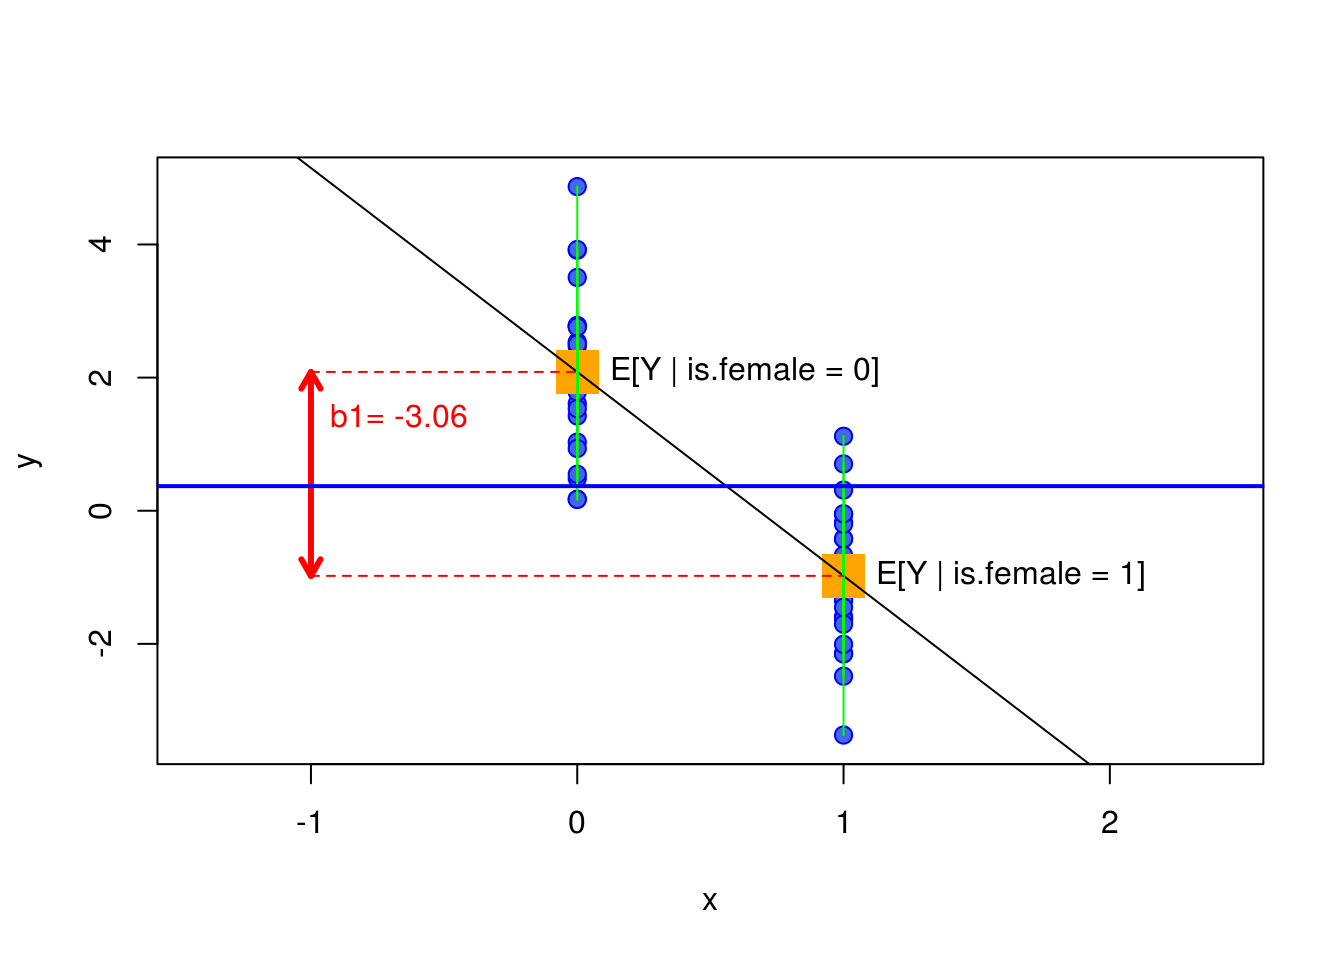
\includegraphics{ScPoEconometrics_files/figure-latex/x-zero-one-1} 

}

\caption{regressing $y \in \mathbb{R}$ on $\text{is.female}_i \in \{0,1\}$. The blue line is $E[y]$, the red arrow is the size of $b_1$. Which is the same as the slope of the regression line in this case and the difference in conditional means!}\label{fig:x-zero-one}
\end{figure}

In figure \ref{fig:x-zero-one} we see that this regression simplifies to
the straight line connecting the mean, or the \emph{expected value} of
\(y\) when \(\text{is.female}_i = 0\), i.e.
\(E[y|\text{is.female}_i=0]\), to the mean when
\(\text{is.female}_i=1\), i.e. \(E[y|\text{is.female}_i=1]\). It is
useful to remember that the \emph{unconditional mean} of \(y\), i.e.
\(E[y]\), is going to be the result of regressing \(y\) only on an
intercept, illustrated by the blue line. This line will always lie in
between both conditional means. As indicated by the red arrow, the
estimate of the coefficient on the dummy, \(b_1\), is equal to the
difference in conditional means for both groups. You should look at our
app now to deepen your understanding of what's going on here:

\begin{Shaded}
\begin{Highlighting}[]
\KeywordTok{library}\NormalTok{(ScPoEconometrics)}
\KeywordTok{launchApp}\NormalTok{(}\StringTok{"reg_dummy"}\NormalTok{)}
\end{Highlighting}
\end{Shaded}

\section{Dummy and Continuous
Variables}\label{dummy-and-continuous-variables}

What happens if there are more predictors than just the dummy variable
in a regression? For example, what if instead we had

\begin{equation}
y_i = b_0 + b_1 \text{is.female}_i + b_2 \text{exper}_i + e_i \label{eq:dummy-reg2}
\end{equation}

where \(\text{exper}_i\) would measure years of experience in the labor
market? As above, the dummy variable acts as an intercept shifter. We
have

\begin{equation}
y_i =  \begin{cases}
b_0 + b_1 + b_2 \times \text{exper}_i + e_i & \text{if is.female=1} \\
b_0  + \hphantom{b_1} +b_2 \times \text{exper}_i + e_i & \text{if is.female=0}
\end{cases}
\end{equation}

so that the intercept is \(b_0 + b_1\) for women but \(b_0\) for men. We
will see this in the real-world example below, but for now let's see the
effect of switching the dummy \emph{on} and \emph{off} in this app:

\begin{Shaded}
\begin{Highlighting}[]
\KeywordTok{library}\NormalTok{(ScPoEconometrics)}
\KeywordTok{launchApp}\NormalTok{(}\StringTok{"reg_dummy_example"}\NormalTok{)}
\end{Highlighting}
\end{Shaded}

\section{\texorpdfstring{Categorical Variables in \texttt{R}:
\texttt{factor}}{Categorical Variables in R: factor}}\label{categorical-variables-in-r-factor}

\texttt{R} has extensive support for categorical variables built-in. The
relevant data type representing a categorical variable is called
\texttt{factor}. We encountered them as basic data types in section
\ref{data-types} already, but it is worth repeating this here. We have
seen that a factor \emph{categorizes} a usually small number of numeric
values by \emph{labels}, as in this example which is similar to what I
used to create regressor \texttt{is.female} for the above regression:

\begin{Shaded}
\begin{Highlighting}[]
\NormalTok{is.female =}\StringTok{ }\KeywordTok{factor}\NormalTok{(}\DataTypeTok{x =} \KeywordTok{c}\NormalTok{(}\DecValTok{0}\NormalTok{,}\DecValTok{1}\NormalTok{,}\DecValTok{1}\NormalTok{,}\DecValTok{0}\NormalTok{), }\DataTypeTok{labels =} \KeywordTok{c}\NormalTok{(}\OtherTok{FALSE}\NormalTok{,}\OtherTok{TRUE}\NormalTok{))}
\NormalTok{is.female}
\end{Highlighting}
\end{Shaded}

\begin{verbatim}
#OUT> [1] FALSE TRUE  TRUE  FALSE
#OUT> Levels: FALSE TRUE
\end{verbatim}

You can see the result is a vector object of type \texttt{factor} with 4
entries, whereby \texttt{0} is represented as \texttt{FALSE} and
\texttt{1} as \texttt{TRUE}. An other example could be if we wanted to
record a variable \emph{sex} instead, and we could do

\begin{Shaded}
\begin{Highlighting}[]
\NormalTok{sex =}\StringTok{ }\KeywordTok{factor}\NormalTok{(}\DataTypeTok{x =} \KeywordTok{c}\NormalTok{(}\DecValTok{0}\NormalTok{,}\DecValTok{1}\NormalTok{,}\DecValTok{1}\NormalTok{,}\DecValTok{0}\NormalTok{), }\DataTypeTok{labels =} \KeywordTok{c}\NormalTok{(}\StringTok{"male"}\NormalTok{,}\StringTok{"female"}\NormalTok{))}
\NormalTok{sex}
\end{Highlighting}
\end{Shaded}

\begin{verbatim}
#OUT> [1] male   female female male  
#OUT> Levels: male female
\end{verbatim}

You can see that this is almost identical, just the \emph{labels} are
different.

\subsection{More Levels}\label{more-levels}

We can go beyond \emph{binary} categorical variables such as
\texttt{TRUE} vs \texttt{FALSE}. For example, suppose that \(x\)
measures educational attainment, i.e.~it is now something like
\(x_i \in \{\text{high school,some college,BA,MSc}\}\). In \texttt{R}
parlance, \emph{high school, some college, BA, MSc} are the
\textbf{levels of factor \(x\)}. A straightforward extension of the
above would dictate to create one dummy variable for each category (or
level), like

\begin{align*}
\text{has.HS}_i &= \mathbf{1}[x_i==\text{high school}] \\
\text{has.someCol}_i &= \mathbf{1}[x_i==\text{some college}] \\
\text{has.BA}_i &= \mathbf{1}[x_i==\text{BA}] \\
\text{has.MSc}_i &= \mathbf{1}[x_i==\text{MSc}] 
\end{align*}

but you can see that this is cumbersome. There is a better solution for
us available:

\begin{Shaded}
\begin{Highlighting}[]
\KeywordTok{factor}\NormalTok{(}\DataTypeTok{x =} \KeywordTok{c}\NormalTok{(}\DecValTok{1}\NormalTok{,}\DecValTok{1}\NormalTok{,}\DecValTok{2}\NormalTok{,}\DecValTok{4}\NormalTok{,}\DecValTok{3}\NormalTok{,}\DecValTok{4}\NormalTok{),}\DataTypeTok{labels =} \KeywordTok{c}\NormalTok{(}\StringTok{"HS"}\NormalTok{,}\StringTok{"someCol"}\NormalTok{,}\StringTok{"BA"}\NormalTok{,}\StringTok{"MSc"}\NormalTok{))}
\end{Highlighting}
\end{Shaded}

\begin{verbatim}
#OUT> [1] HS      HS      someCol MSc     BA      MSc    
#OUT> Levels: HS someCol BA MSc
\end{verbatim}

Notice here that \texttt{R} will apply the labels in increasing order
the way you supplied it (i.e.~a numerical value \texttt{4} will
correspond to ``MSc'', no matter the ordering in \texttt{x}.)

\subsection{\texorpdfstring{\texttt{factor} and
\texttt{lm()}}{factor and lm()}}\label{factor-and-lm}

The above developed \texttt{factor} terminology fits neatly into
\texttt{R}'s linear model fitting framework. Let us illustrate the
simplest use by way of example.

\begin{Shaded}
\begin{Highlighting}[]
\KeywordTok{library}\NormalTok{(Ecdat)  }\CommentTok{# need to load this library}
\KeywordTok{data}\NormalTok{(}\StringTok{"Wages"}\NormalTok{)   }\CommentTok{# from Ecdat}
\KeywordTok{str}\NormalTok{(Wages)   }\CommentTok{# let's examine this dataset!}
\end{Highlighting}
\end{Shaded}

\begin{verbatim}
#OUT> 'data.frame': 4165 obs. of  12 variables:
#OUT>  $ exp    : int  3 4 5 6 7 8 9 30 31 32 ...
#OUT>  $ wks    : int  32 43 40 39 42 35 32 34 27 33 ...
#OUT>  $ bluecol: Factor w/ 2 levels "no","yes": 1 1 1 1 1 1 1 2 2 2 ...
#OUT>  $ ind    : int  0 0 0 0 1 1 1 0 0 1 ...
#OUT>  $ south  : Factor w/ 2 levels "no","yes": 2 2 2 2 2 2 2 1 1 1 ...
#OUT>  $ smsa   : Factor w/ 2 levels "no","yes": 1 1 1 1 1 1 1 1 1 1 ...
#OUT>  $ married: Factor w/ 2 levels "no","yes": 2 2 2 2 2 2 2 2 2 2 ...
#OUT>  $ sex    : Factor w/ 2 levels "female","male": 2 2 2 2 2 2 2 2 2 2 ...
#OUT>  $ union  : Factor w/ 2 levels "no","yes": 1 1 1 1 1 1 1 1 1 2 ...
#OUT>  $ ed     : int  9 9 9 9 9 9 9 11 11 11 ...
#OUT>  $ black  : Factor w/ 2 levels "no","yes": 1 1 1 1 1 1 1 1 1 1 ...
#OUT>  $ lwage  : num  5.56 5.72 6 6 6.06 ...
\end{verbatim}

Notice here that, conveniently, \texttt{sex} is already coded as type
\texttt{factor}. Now assume that this is a single cross section for
wages of US workers. The main outcome variable is \texttt{lwage} which
stands for \emph{logarithm of wage}.

\subsection{Log Transformations}\label{log-transformations}

It is quite common to transform either outcome or explanatory or both
variables by the natural logarithm. The primary motivation of this is to
make the regression scale invariant. Suppose that factor \(\alpha\)
represented the \emph{scale} of measurement of income, so that
\(\alpha=1\) if we measure in Euros, or \(\alpha=1000\) if in thousands
of Euros. With log-transforming regressor \(x\), our equation would look
like

\[
y = b_0 + b_1 \log(\alpha x) = b_0 + \log \alpha  + b_1 \log x 
\] where the \emph{scale} \(\alpha\) moves into the intercept, and our
slope coefficient becomes invariant to it. If both outcome and regressor
are transformed, we have

\[
\log y = b_0 + b_1 \log x
\] and the slope coefficient is

\[
b_1 = \frac{d\log y}{d \log x} = \frac{dy/y}{dx/x}
\] which represents the \textbf{elasticity} of \(y\) with respect to
\(x\): what is the percentage change in \(y\) if \(x\) changes by one
percent?

Finally, if \emph{only the outcome} is log transformed, but not the
regressor, we have a \emph{semi-elasticity} formulation. \[
\log y = b_0 + b_1 x
\] and the slope coefficient becomes

\[
b_1 = \frac{d\log y}{d x}
\] This means a one-unit change in \(x\) increases the logarithm of the
outcome by \(b_1\) units. For small changes in \(x\), we can just
exponentiate \(b_1\) to get the effect of \(x\) the \emph{level} of
\(y\).

Going back to our example, let's say that a workers wage depends only on
his \emph{experience}, measured in the number of years he/she worked
full-time:

\begin{equation}
\ln w_i = b_0 + b_1 exp_i + e_i \label{eq:wage-exp}
\end{equation}

\begin{Shaded}
\begin{Highlighting}[]
\NormalTok{lm_w =}\StringTok{ }\KeywordTok{lm}\NormalTok{(lwage }\OperatorTok{~}\StringTok{ }\NormalTok{exp, }\DataTypeTok{data =}\NormalTok{ Wages)}
\KeywordTok{summary}\NormalTok{(lm_w)}
\end{Highlighting}
\end{Shaded}

\begin{verbatim}
#OUT> 
#OUT> Call:
#OUT> lm(formula = lwage ~ exp, data = Wages)
#OUT> 
#OUT> Residuals:
#OUT>      Min       1Q   Median       3Q      Max 
#OUT> -2.30153 -0.29144  0.02307  0.27927  1.97171 
#OUT> 
#OUT> Coefficients:
#OUT>              Estimate Std. Error t value Pr(>|t|)    
#OUT> (Intercept) 6.5014318  0.0144657  449.44   <2e-16 ***
#OUT> exp         0.0088101  0.0006378   13.81   <2e-16 ***
#OUT> ---
#OUT> Signif. codes:  0 '***' 0.001 '**' 0.01 '*' 0.05 '.' 0.1 ' ' 1
#OUT> 
#OUT> Residual standard error: 0.4513 on 4163 degrees of freedom
#OUT> Multiple R-squared:  0.04383, Adjusted R-squared:  0.0436 
#OUT> F-statistic: 190.8 on 1 and 4163 DF,  p-value: < 2.2e-16
\end{verbatim}

We see from this that an additional year of full-time work experience
will increase the mean of \(\ln w\) by 0.0088. Given the log
transformation on wages, we can just exponentiate that to get an
estimated effect on the (geometric!) mean of wages as
\(\exp(\hat{b}_1) = 1.0088491\). This means that hourly wages increase
by roughly \(100 * (\exp(b_1)-1) = 0.88\) percent with an additional
year of experience. We can verify the positive relationship in figure
\ref{fig:wage-plot}.

\begin{figure}

{\centering 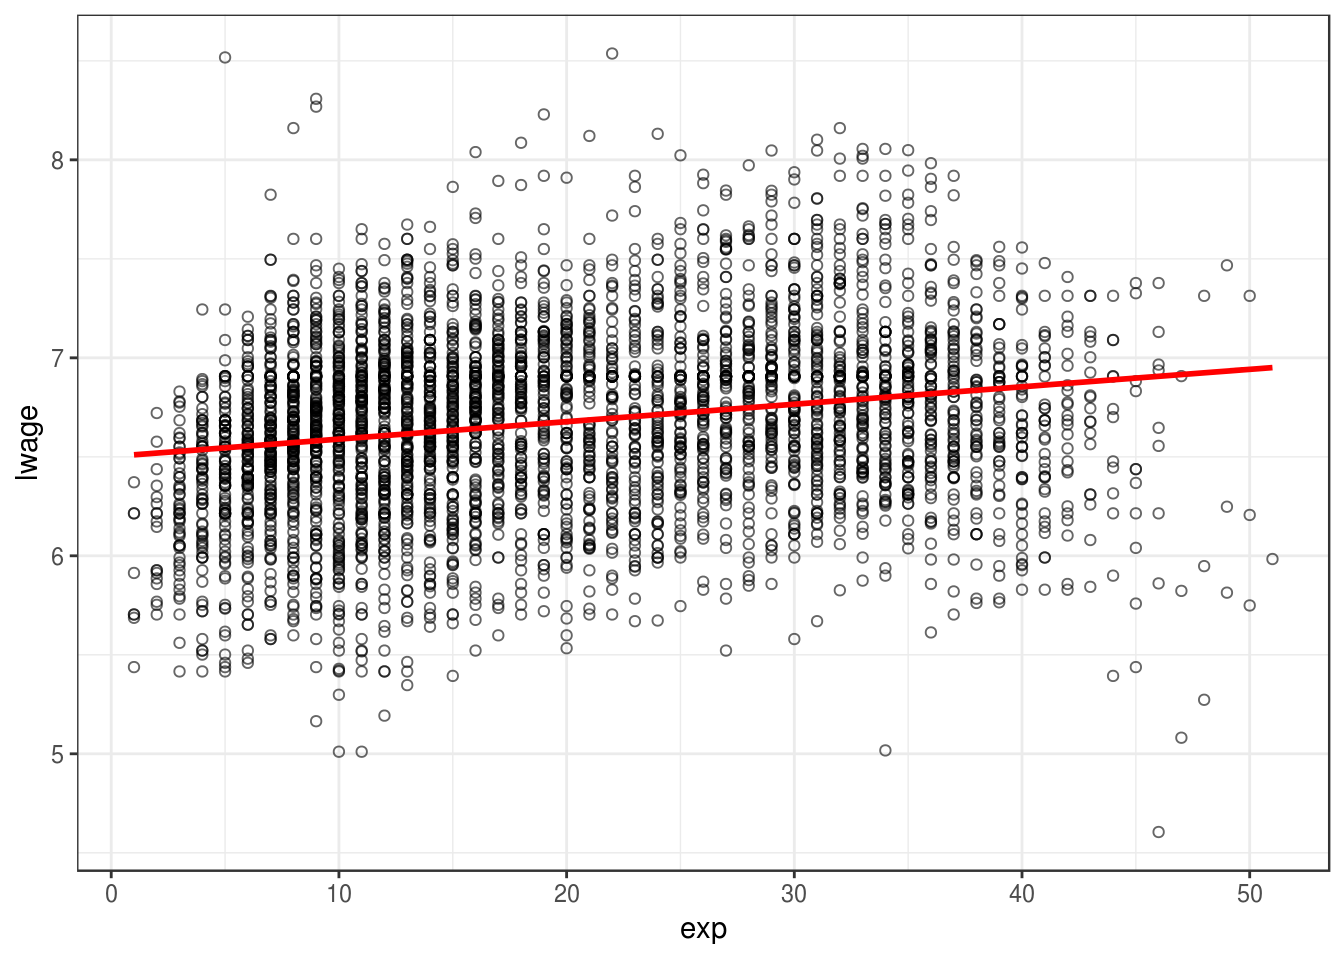
\includegraphics{ScPoEconometrics_files/figure-latex/wage-plot-1} 

}

\caption{log wage vs experience. Red line shows the regression.}\label{fig:wage-plot}
\end{figure}

Now let's investigate whether this relationship is different for men and
women. We can do this by just including the \texttt{factor} variable
\texttt{sex}:

\begin{equation}
\ln w_i = b_0 + b_1 exp_i + b_2 sex_i + e_i \label{eq:wage-sex}
\end{equation}

In \texttt{R} we can do this easily by using the \texttt{update}
function as follows:

\begin{Shaded}
\begin{Highlighting}[]
\NormalTok{lm_sex =}\StringTok{ }\KeywordTok{update}\NormalTok{(lm_w, . }\OperatorTok{~}\StringTok{ }\NormalTok{. }\OperatorTok{+}\StringTok{ }\NormalTok{sex)  }\CommentTok{# update lm_w with same LHS, same RHS, but add sex to it}
\KeywordTok{summary}\NormalTok{(lm_sex)}
\end{Highlighting}
\end{Shaded}

\begin{verbatim}
#OUT> 
#OUT> Call:
#OUT> lm(formula = lwage ~ exp + sex, data = Wages)
#OUT> 
#OUT> Residuals:
#OUT>      Min       1Q   Median       3Q      Max 
#OUT> -1.87081 -0.26688  0.01733  0.26336  1.90325 
#OUT> 
#OUT> Coefficients:
#OUT>              Estimate Std. Error t value Pr(>|t|)    
#OUT> (Intercept) 6.1257661  0.0223319  274.31   <2e-16 ***
#OUT> exp         0.0076134  0.0006082   12.52   <2e-16 ***
#OUT> sexmale     0.4501101  0.0210974   21.34   <2e-16 ***
#OUT> ---
#OUT> Signif. codes:  0 '***' 0.001 '**' 0.01 '*' 0.05 '.' 0.1 ' ' 1
#OUT> 
#OUT> Residual standard error: 0.4286 on 4162 degrees of freedom
#OUT> Multiple R-squared:  0.1381,  Adjusted R-squared:  0.1377 
#OUT> F-statistic: 333.4 on 2 and 4162 DF,  p-value: < 2.2e-16
\end{verbatim}

What's going on here? Remember from above that \texttt{sex} is a
\texttt{factor} with 2 levels \emph{female} and \emph{male}. We see in
the above output that \texttt{R} included a regressor called
\texttt{sexmale} \(=\mathbf{1}[sex_i==male]\). This is a combination of
the variable name \texttt{sex} and the level which was included in the
regression. In other words, \texttt{R} chooses a \emph{reference
category} (by default the first of all levels by order of appearance),
which is excluded - here this is \texttt{sex=="female"}. The
interpretation is that \(b_2\) measures the effect of being male
\emph{relative} to being female. \texttt{R} automatically creates a
dummy variable for each potential level, excluding the first category.
In particular, if \texttt{sex} had a third category
\texttt{dont\ want\ to\ say}, there would be an additional regressor
called \texttt{sexdontwanttosay}.

\begin{figure}

{\centering 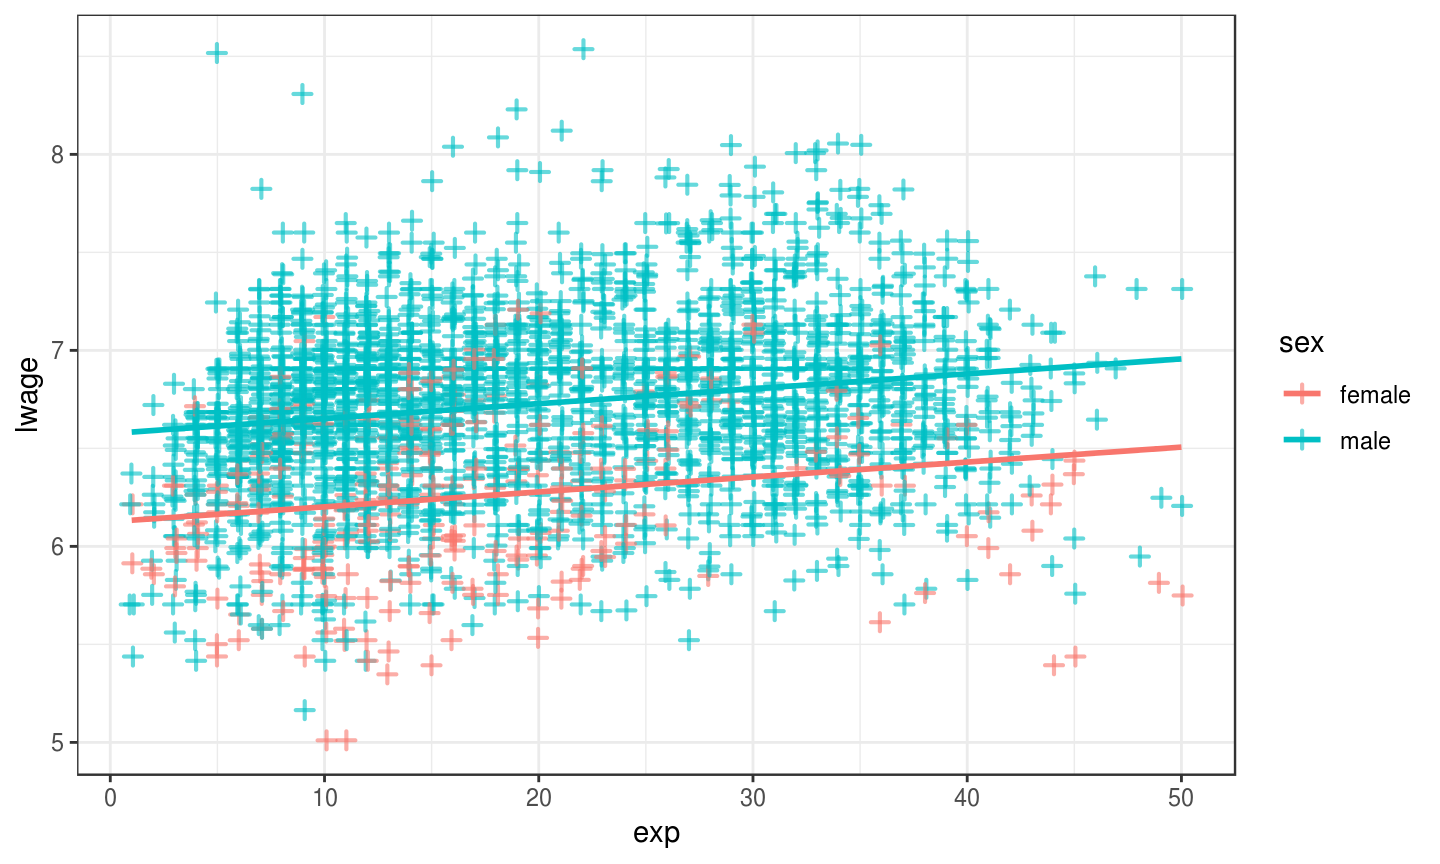
\includegraphics{ScPoEconometrics_files/figure-latex/wage-plot2-1} 

}

\caption{log wage vs experience with different intercepts by sex}\label{fig:wage-plot2}
\end{figure}

Figure \ref{fig:wage-plot2} illustrates this. You can see that both male
and female have the same upward sloping regression line. But you can
also see that there is a parallel downward shift from male to female
line. The estimate of \(b_2 = 0.45\) is the size of the downward shift.

\section{Saturated Models: Main Effects and
Interactions}\label{saturated-models-main-effects-and-interactions}

You can see above that we \emph{restricted} male and female to have the
same slope with repect to years of experience. This may or may not be a
good assumption. Thankfully, the dummy variable regression machinery
allows for a quick solution to this - so-called \emph{interaction}
effects. As already introduced in chapter \ref{mreg-interactions},
interactions allow that the \emph{ceteris paribus} effect of a certain
regressor, \texttt{exp} say, depends also on the value of yet another
regressor, \texttt{sex} for example. Suppose then we would like to see
whether male and female not only have different intercepts, but also
different slopes with respect to \texttt{exp} in figure
\ref{fig:wage-plot2}. Therefore we formulate this version of our model:

\begin{equation}
\ln w_i = b_0 + b_1 exp_i + b_2 sex_i + b_3 (sex_i \times exp_i) + e_i \label{eq:wage-sex-inter}
\end{equation}

The inclusion of the \emph{product} of \texttt{exp} and \texttt{sex}
amounts to having different slopes for different categories in
\texttt{sex}. This is easy to see if we take the partial derivative of
\eqref{eq:wage-sex-inter} with respect to \texttt{sex}:

\begin{equation}
\frac{\partial \ln w_i}{\partial sex_i} = b_2 + b_3 exp_i \label{eq:wage-sex-inter-deriv}
\end{equation}

Back in our \texttt{R} session, we can run the full interactions model
like this:

\begin{Shaded}
\begin{Highlighting}[]
\NormalTok{lm_inter =}\StringTok{ }\KeywordTok{lm}\NormalTok{(lwage }\OperatorTok{~}\StringTok{ }\NormalTok{exp}\OperatorTok{*}\NormalTok{sex, }\DataTypeTok{data =}\NormalTok{ Wages)}
\KeywordTok{summary}\NormalTok{(lm_inter)}
\end{Highlighting}
\end{Shaded}

\begin{verbatim}
#OUT> 
#OUT> Call:
#OUT> lm(formula = lwage ~ exp * sex, data = Wages)
#OUT> 
#OUT> Residuals:
#OUT>      Min       1Q   Median       3Q      Max 
#OUT> -1.82137 -0.26797  0.01781  0.26231  1.90757 
#OUT> 
#OUT> Coefficients:
#OUT>             Estimate Std. Error t value Pr(>|t|)    
#OUT> (Intercept) 6.169017   0.038165 161.643  < 2e-16 ***
#OUT> exp         0.005071   0.001918   2.644  0.00822 ** 
#OUT> sexmale     0.401116   0.040917   9.803  < 2e-16 ***
#OUT> exp:sexmale 0.002826   0.002022   1.397  0.16236    
#OUT> ---
#OUT> Signif. codes:  0 '***' 0.001 '**' 0.01 '*' 0.05 '.' 0.1 ' ' 1
#OUT> 
#OUT> Residual standard error: 0.4285 on 4161 degrees of freedom
#OUT> Multiple R-squared:  0.1385,  Adjusted R-squared:  0.1379 
#OUT> F-statistic:   223 on 3 and 4161 DF,  p-value: < 2.2e-16
\end{verbatim}

You can see here that \texttt{R} automatically expands \texttt{exp*sex}
to include both \emph{main effects}, i.e. \texttt{exp} and \texttt{sex}
as single regressors as before, and their interaction, denoted by
\texttt{exp:sexmale}. It turns out that in this example, the estimate
for the interaction is not statistically significant, i.e.~we cannot
reject the null hypothesis that \(b_3 = 0\). (If, for some reason, you
wanted to include only the interaction, you could supply directly
\texttt{formula\ =\ lwage\ \textasciitilde{}\ exp:sex} to \texttt{lm},
although this would be a rather difficult to interpret model.)

We call a model like \eqref{eq:wage-sex-inter} a \emph{saturated model},
because it includes all main effects and possible interactions. What our
little exercise showed us was that with the sample of data at hand, we
cannot actually claim that there exists a differential slope for male
and female, so the model with main effects only may be more appropriate
here.

To finally illustrate the limits of interpretability when including
interactions, suppose we run the fully saturated model for \texttt{sex},
\texttt{smsa}, \texttt{union} and \texttt{bluecol}, including all main
and all interaction effects:

\begin{Shaded}
\begin{Highlighting}[]
\NormalTok{lm_full =}\StringTok{ }\KeywordTok{lm}\NormalTok{(lwage }\OperatorTok{~}\StringTok{ }\NormalTok{sex}\OperatorTok{*}\NormalTok{smsa}\OperatorTok{*}\NormalTok{union}\OperatorTok{*}\NormalTok{bluecol,}\DataTypeTok{data=}\NormalTok{Wages)}
\KeywordTok{summary}\NormalTok{(lm_full)}
\end{Highlighting}
\end{Shaded}

\begin{verbatim}
#OUT> 
#OUT> Call:
#OUT> lm(formula = lwage ~ sex * smsa * union * bluecol, data = Wages)
#OUT> 
#OUT> Residuals:
#OUT>      Min       1Q   Median       3Q      Max 
#OUT> -1.95214 -0.23409 -0.01681  0.25317  1.90450 
#OUT> 
#OUT> Coefficients:
#OUT>                                     Estimate Std. Error t value Pr(>|t|)
#OUT> (Intercept)                          6.12378    0.06300  97.198  < 2e-16
#OUT> sexmale                              0.67057    0.06577  10.195  < 2e-16
#OUT> smsayes                              0.33424    0.06872   4.864 1.19e-06
#OUT> unionyes                             0.84284    0.16866   4.997 6.06e-07
#OUT> bluecolyes                          -0.34016    0.08423  -4.039 5.47e-05
#OUT> sexmale:smsayes                     -0.15917    0.07226  -2.203 0.027670
#OUT> sexmale:unionyes                    -0.92893    0.17816  -5.214 1.94e-07
#OUT> smsayes:unionyes                    -0.83927    0.17979  -4.668 3.14e-06
#OUT> sexmale:bluecolyes                  -0.15046    0.08820  -1.706 0.088100
#OUT> smsayes:bluecolyes                  -0.12471    0.09727  -1.282 0.199882
#OUT> unionyes:bluecolyes                 -0.31819    0.22924  -1.388 0.165208
#OUT> sexmale:smsayes:unionyes             0.72672    0.19060   3.813 0.000139
#OUT> sexmale:smsayes:bluecolyes           0.25860    0.10327   2.504 0.012318
#OUT> sexmale:unionyes:bluecolyes          0.71906    0.23772   3.025 0.002503
#OUT> smsayes:unionyes:bluecolyes          0.50057    0.24862   2.013 0.044137
#OUT> sexmale:smsayes:unionyes:bluecolyes -0.58330    0.25899  -2.252 0.024361
#OUT>                                        
#OUT> (Intercept)                         ***
#OUT> sexmale                             ***
#OUT> smsayes                             ***
#OUT> unionyes                            ***
#OUT> bluecolyes                          ***
#OUT> sexmale:smsayes                     *  
#OUT> sexmale:unionyes                    ***
#OUT> smsayes:unionyes                    ***
#OUT> sexmale:bluecolyes                  .  
#OUT> smsayes:bluecolyes                     
#OUT> unionyes:bluecolyes                    
#OUT> sexmale:smsayes:unionyes            ***
#OUT> sexmale:smsayes:bluecolyes          *  
#OUT> sexmale:unionyes:bluecolyes         ** 
#OUT> smsayes:unionyes:bluecolyes         *  
#OUT> sexmale:smsayes:unionyes:bluecolyes *  
#OUT> ---
#OUT> Signif. codes:  0 '***' 0.001 '**' 0.01 '*' 0.05 '.' 0.1 ' ' 1
#OUT> 
#OUT> Residual standard error: 0.3832 on 4149 degrees of freedom
#OUT> Multiple R-squared:  0.3129,  Adjusted R-squared:  0.3105 
#OUT> F-statistic:   126 on 15 and 4149 DF,  p-value: < 2.2e-16
\end{verbatim}

The main effects remain clear to interpret: being a blue collar worker,
for example, reduces average wages by 34\% relative to white collar
workers. One-way interactions are still ok to interpret as well:
\texttt{sexmale:bluecolyes} indicates in addition to a wage premium over
females of 0.67, and a penalty of being blue collar of -0.34,
\textbf{male} blue collar workers suffer an additional wage loss of
-0.15. All of this is relative to the base category, which are female
white collar workers who don't live in an smsa and are not union
members. If we now add a third or even a fourth interaction, this
becomes much harder to interpret, and in fact we rarely see such
interactions in applied work.

\chapter{Standard Errors}\label{std-errors}

In the previous chapters we have seen how the OLS method can produce
estimates about intercept and slope coefficients from data. You have
seen this method at work in \texttt{R} by using the \texttt{lm} function
as well. It is now time to introduce the notion that given that \(b_0\),
\(b_1\) and \(b_2\) are \emph{estimates} of some unkown \emph{population
parameters}, there is some degree of \textbf{uncertainty} about their
values. An other way to say this is that we want some indication about
the \emph{precision} of those estimates.

\begin{note}
How \emph{confident} should we be about the estimated values \(b\)?
\end{note}

 Let's go back to the regression with one variable and remind ourselves
of the example at the end of chapter \ref{linreg}. There we introduced
the term \emph{confidence interval}, shown as the shaded area in figure
\ref{fig:confint}:

\begin{figure}

{\centering 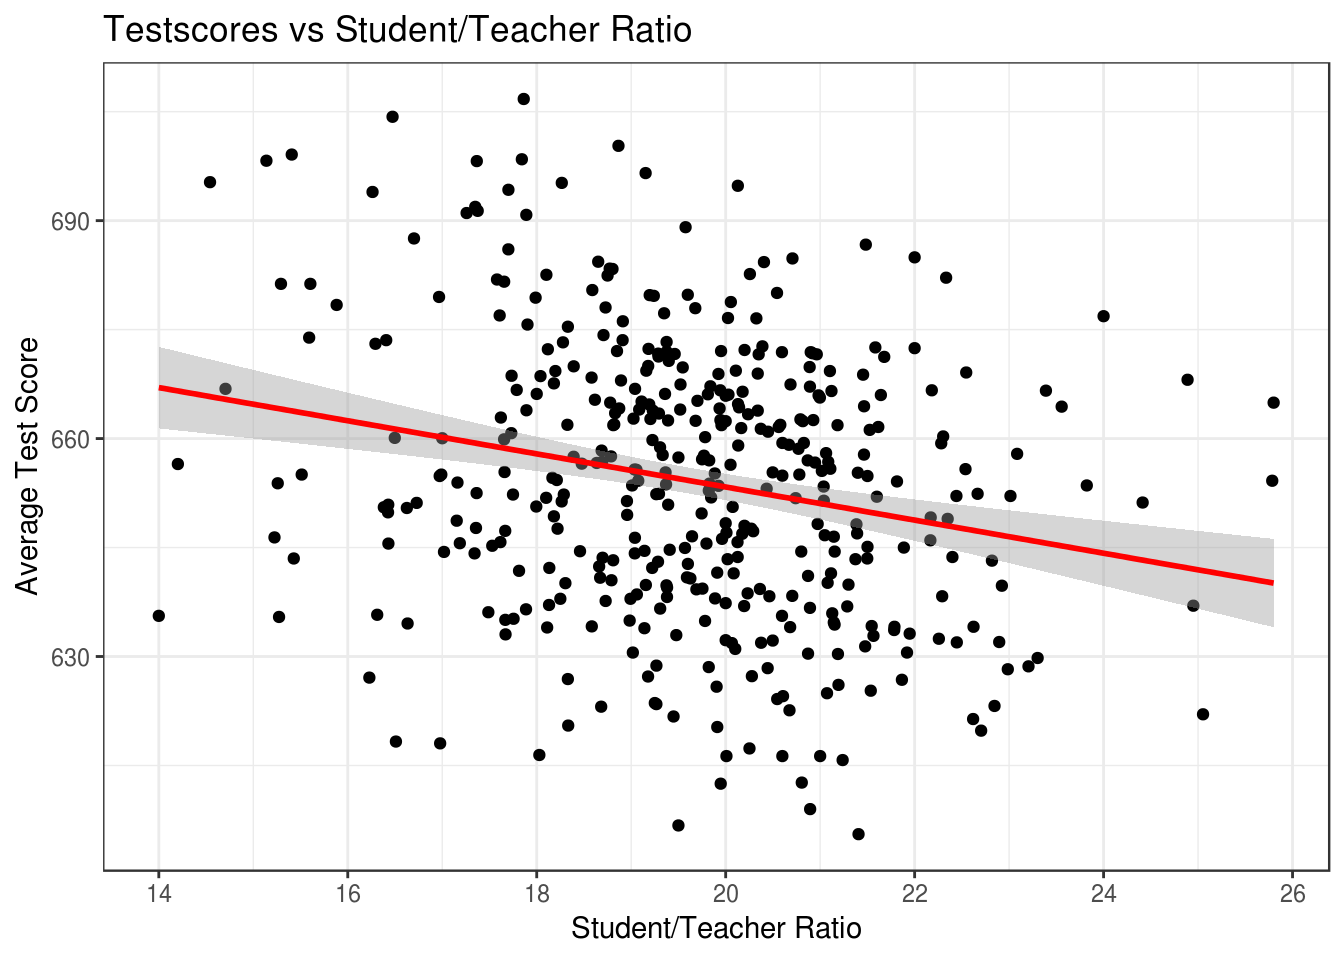
\includegraphics{ScPoEconometrics_files/figure-latex/confint-1} 

}

\caption{Confidence bands around a regression line.}\label{fig:confint}
\end{figure}

The shaded area shows us the region within which the \textbf{true} red
line will lie with 95\% probability. The fact that there is an unknown
true line (i.e.~a \emph{true} slope coefficient \(\beta_1\)) that we
wish to uncover from a sample of data should remind you immediately of
our first tutorial. There, we wanted to estimate the true population
mean from a sample of data, and we saw that as the sample size \(N\)
increased, our estimate got better and better - fundamentally this is
the same idea here.

\section{\texorpdfstring{What is \emph{true}? What are Statistical
Models?}{What is true? What are Statistical Models?}}\label{what-is-true-what-are-statistical-models}

A \textbf{statistical model} is simply a set of assumptions about how
some data have been generated. As such, it models the data-generating
process (DGP), as we have it in mind. Once we define a DGP, we could
simulate data from it and see how this compares to the data we observe
in the real world. Or, we could change the parameters of the DGP so as
to understand how the real world data \emph{would} change, could we (or
some policy) change the corresponding parameters in reality. Let us now
consider one particular statistical model, which in fact we have seen so
many times already.

\section{The Classical Regression Model}\label{class-reg}

Let's bring back our simple model \eqref{eq:abline} to explain this
concept.

\begin{equation}
y_i = \beta_0 + \beta_1 x_i + \varepsilon_i \label{eq:abline-5}
\end{equation}

The smallest set of assumptions used to define the \emph{classical
regression model} as in \eqref{eq:abline-5} are the following:

\begin{enumerate}
\def\labelenumi{\arabic{enumi}.}
\tightlist
\item
  The data are \textbf{not linearly dependent}: Each variable provides
  new information for the outcome, and it cannot be replicated as a
  linear combination of other variables. We have seen this in section
  \ref{multicol}. In the particular case of one regressor, as here, we
  require that \(x\) exhibit some variation in the data, i.e.
  \(Var(x)\neq 0\).
\item
  The mean of the residuals conditional on \(x\) should be zero,
  \(E[\varepsilon|x] = 0\). Notice that this also means that
  \(Cov(\varepsilon,x) = 0\), i.e.~that the errors and our explanatory
  variable(s) should be \emph{uncorrelated}. It is said that \(x\)
  should be \textbf{strictly exogenous} to the model.
\end{enumerate}

These assumptions are necessary to successfully (and correctly!) run an
OLS regression. They are often supplemented with an additional set of
assumptions, which help with certain aspects of the exposition, but are
not strictly necessary:

\begin{enumerate}
\def\labelenumi{\arabic{enumi}.}
\setcounter{enumi}{2}
\tightlist
\item
  The data are drawn from a \textbf{random sample} of size \(n\):
  observation \((x_i,y_i)\) comes from the exact same distribution, and
  is independent of observation \((x_j,y_j)\), for all \(i\neq j\).
\item
  The variance of the error term \(\varepsilon\) is the same for each
  value of \(x\): \(Var(\varepsilon|x) = \sigma^2\). This property is
  called \textbf{homoskedasticity}.
\item
  The error is normally distributed, i.e.
  \(\varepsilon \sim \mathcal{N}(0,\sigma^2)\)
\end{enumerate}

Invoking assumption 5. in particular defines what is commonly called the
\emph{normal} linear regression model.

\subsection{\texorpdfstring{\(b\) is not
\(\beta\)!}{b is not \textbackslash{}beta!}}\label{b-is-not-beta}

Let's talk about the small but important modifications we applied to
model \eqref{eq:abline} to end up at \eqref{eq:abline-5} above:

\begin{itemize}
\tightlist
\item
  \(\beta_0\) and \(\beta_1\) and intercept and slope parameters
\item
  \(\varepsilon\) is the error term.
\end{itemize}

First, we \emph{assumed} that \eqref{eq:abline-5} is the correct
represenation of the DGP. With that assumption in place, the values
\(\beta_0\) and \(\beta_1\) are the \emph{true parameter values} which
generated the data. Notice that \(\beta_0\) and \(\beta_1\) are
potentially different from \(b_0\) and \(b_1\) in \eqref{eq:abline} for a
given sample of data - they could in practice be very close to each
other, but \(b_0\) and \(b_1\) are \emph{estimates} of \(\beta_0\) and
\(\beta_1\). And, crucially, those estimates are generated from a sample
of data. Now, the fact that our data \(\{y_i,x_i\}_{i=1}^N\) are a
sample from a larger population, means that there will be \emph{sampling
variation} in our estimates - exactly like in the case of the sample
mean estimating the population average as mentioned above. One
particular sample of data will generate one particular set of estimates
\(b_0\) and \(b_1\), whereas another sample of data will generate
estimates which will in general be different - by \emph{how much} those
estimates differ across samples is the question in this chapter. In
general, the more observations we have the greater the precision of our
estimates, hence, the closer the estimates from different samples will
lie together.

\subsection{Standard Errors in Theory}\label{se-theory}

The standard deviation of the OLS parameters is generally called
\emph{standard error}. As such, it is just the square root of the
parameter's variance. Under assumptions 1. through 4. we can define the
formula for the variance of our slope coefficient in the context of our
single regressor model \eqref{eq:abline-5} as follows:

\begin{equation}
Var(b_1|x_i) = \frac{\sigma^2}{\sum_i^N (x_i - \bar{x})^2}  \label{eq:var-ols}
\end{equation}

In pratice, we don't know the theoretical variance of \(\varepsilon\),
i.e. \(\sigma^2\), but we form an estimate about it from our sample of
data. A widely used estimate uses the already encountered SSR (sum of
squared residuals), and is denoted \(s^2\):

\[
s^2 = \frac{SSR}{n-p} = \frac{\sum_{i=1}^n (y_i - b_0 - b_1 x_i)^2}{n-p} =  \frac{\sum_{i=1}^n e_i^2}{n-p}
\] where \(n-p\) are the \emph{degrees of freedom} available in this
estimation. \(p\) is the number of parameters we wish to estimate (here:
1). So, the variance formula would become

\begin{equation}
Var(b_1|x_i) = \frac{SSR}{(n-p)\sum_i^N (x_i - \bar{x})^2}  \label{eq:var-ols2}
\end{equation}

We most of the time work directly with the \emph{standard error} of a
coefficient, hence we define

\begin{equation}
SE(b_1) = \sqrt{Var(b_1|x_i)} = \sqrt{\frac{SSR}{(n-p)\sum_i^N (x_i - \bar{x})^2}}  \label{eq:SE-ols2}
\end{equation}

You can clearly see that, as \(n\) increases, the denominator increases,
and therefore variance and standard error of the estimate will decrease.

\subsection{Standard Errors in
Practice}\label{standard-errors-in-practice}

We would like to further make this point in an experiential way, i.e.~we
want you to experience what is going on. We invite you to spend some
time with the following apps. In particular, make sure you have a
thorough understanding of \texttt{launchApp("estimate")}.

\begin{Shaded}
\begin{Highlighting}[]
\KeywordTok{library}\NormalTok{(ScPoEconometrics)}
\KeywordTok{launchApp}\NormalTok{(}\StringTok{"estimate"}\NormalTok{)}
\KeywordTok{launchApp}\NormalTok{(}\StringTok{"sampling"}\NormalTok{)  }
\KeywordTok{launchApp}\NormalTok{(}\StringTok{"standard_errors_simple"}\NormalTok{) }
\KeywordTok{launchApp}\NormalTok{(}\StringTok{"standard_errors_changeN"}\NormalTok{) }
\end{Highlighting}
\end{Shaded}

\section{Back to Sampling}\label{back-to-sampling}

Imagine we were tasked by the Director of our school to provide him with
our best guess of the \emph{mean body height} \(\mu\) amongst all
SciencesPo students in order to assess which height the new desks should
have. Of course, we are econometricians and don't \emph{guess} things:
we \textbf{estimate} them! How would we go about this task and estimate
\(\mu\)?

You may want to ask: Why bother with this estimation business at all,
and not just measure all students' height, compute \(\mu\), and that's
it? That's a good question! In most cases, we cannot do this, either
because we do not have access to the entire population (think of
computing the mean height of all Europeans!), or it's too costly to
measure everyone, or it's impractical. That's why we take \emph{samples}
from the wider population, to make inference. In our example, suppose
we'd randomly measure students coming out of the SciencesPo building at
27 Rue Saint Guillaume until we have \(50\) measurements on any given
Monday. Suppose further that we found a sample mean height
\(\bar{x} = 168.5\), and that the sample standard deviation was
\(s=10\). In short, we found the data summarized in figure
\ref{fig:heightdata}

\begin{figure}

{\centering 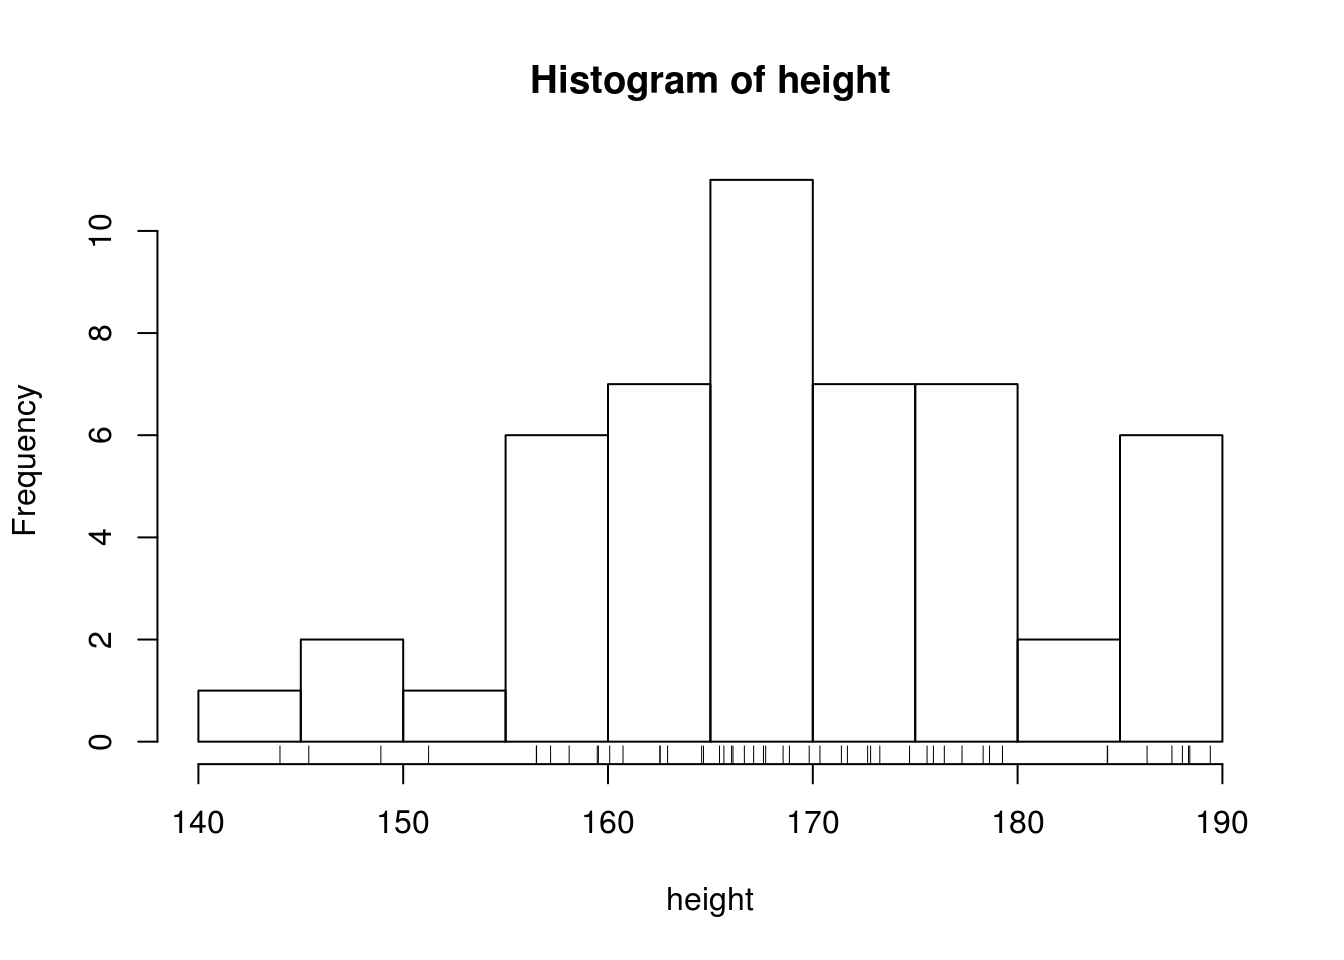
\includegraphics{ScPoEconometrics_files/figure-latex/heightdata-1} 

}

\caption{Our ficitious sample of SciencesPo students' body height. The small ticks indicate the location of each measurement.}\label{fig:heightdata}
\end{figure}

What are we going to tell \emph{Monsieur le Directeur} now, with those
two numbers and figure \ref{fig:heightdata} in hand? Before we address
this issue, we need to make a short detour into \emph{test statistics}.

\subsection{Test Statistics}\label{test-statistics}

We have encountered many statistics already: think of the sample mean,
or the standard deviation. Statistics are just functions of data.
\emph{Test} statistics are used to perform statistical tests.

Many test statistics rely on some notion of \emph{standardizing} the
sample data so that it becomes comparable to a theoretical distribution.
We encountered this idea already in section \ref{reg-standard}, where we
talked about a standardized regression. The most common standardization
is the so-called \emph{z-score}, which says that

\begin{equation}
\frac{x - \mu}{\sigma}\equiv z\sim \mathcal{N}(0,1), \label{eq:zscore}
\end{equation}

in other words, substracting the population mean from random variable
\(x\) and dividing by it's population standard deviation yields a
standard normally distributed random variable, commonly called \(z\).

A very similar idea applies if we \emph{don't know} the population
variance (which is our case here!). The corresponding standardization
gives rise to the \emph{t-statistic}, and it looks very similar to
\eqref{eq:zscore}:

\begin{equation}
\sqrt{n} \frac{\bar{x} - \mu}{s} \equiv T \sim t_{n-1} \label{eq:tscore}
\end{equation}

Several things to note:

\begin{itemize}
\tightlist
\item
  We observe the same standardization as above: dividing by the sample
  standard deviation \(s\) brings \(\bar{x} - \mu\) to a \emph{unit
  free} scale.
\item
  We use \(\bar{x}\) and \(s\) instead of \(x\) and \(\sigma\)
\item
  We multiply by \(\sqrt{n}\) because we expect \(\bar{x} - \mu\) to be
  a small number: we need to \emph{rescale} it again to make it
  compatible with the \(t_{n-1}\) distribution.
\item
  \(t_{n-1}\) is the
  \href{https://en.wikipedia.org/wiki/Student's_t-distribution}{Student's
  T} distribution with \(n-1\) degrees of freedom. We don't have \(n\)
  degrees of freedom because we already had to estimate one statistic
  (\(\bar{x}\)) in order to construct \(T\).
\end{itemize}

\subsection{Confidence Intervals}\label{CI}

Back to our example now! We are clearly in need of some measure of
\emph{confidence} about our sample statistic \(\bar{x} = 168.5\) before
we communicate our result. It seems reasonable to inform the Director
about \(\bar{x}\), but surely we also need to tell him that there was
considerable \emph{dispersion} in the data: Some people were as short as
143.98cm, while others were as tall as 189.41cm!

The way to proceed is to construct a \emph{confidence interval} about
the true population mean \(\mu\), based on \(\bar{x}\), which will take
this uncertainty into account. We will use the \emph{t} statistic from
above. We want to have a \emph{symmetric interval} around \(\bar{x}\)
which contains the true value \(\mu\) with probability \(1-\alpha\). One
very popular choice of \(\alpha\) is \(0.05\), hence we cover \(\mu\)
with 95\% probability. After computing our statistic \(T\) as defind in
\eqref{eq:tscore}, this interval is defined as follows:

\begin{align}
\Pr \left(-c \leq T \leq c \right) = 1-\alpha \label{eq:ci}
\end{align}

where \(c\) stands for \emph{critical value}, which we need to choose.
This is illustrated in figure \ref{fig:cifig}.

\begin{figure}

{\centering 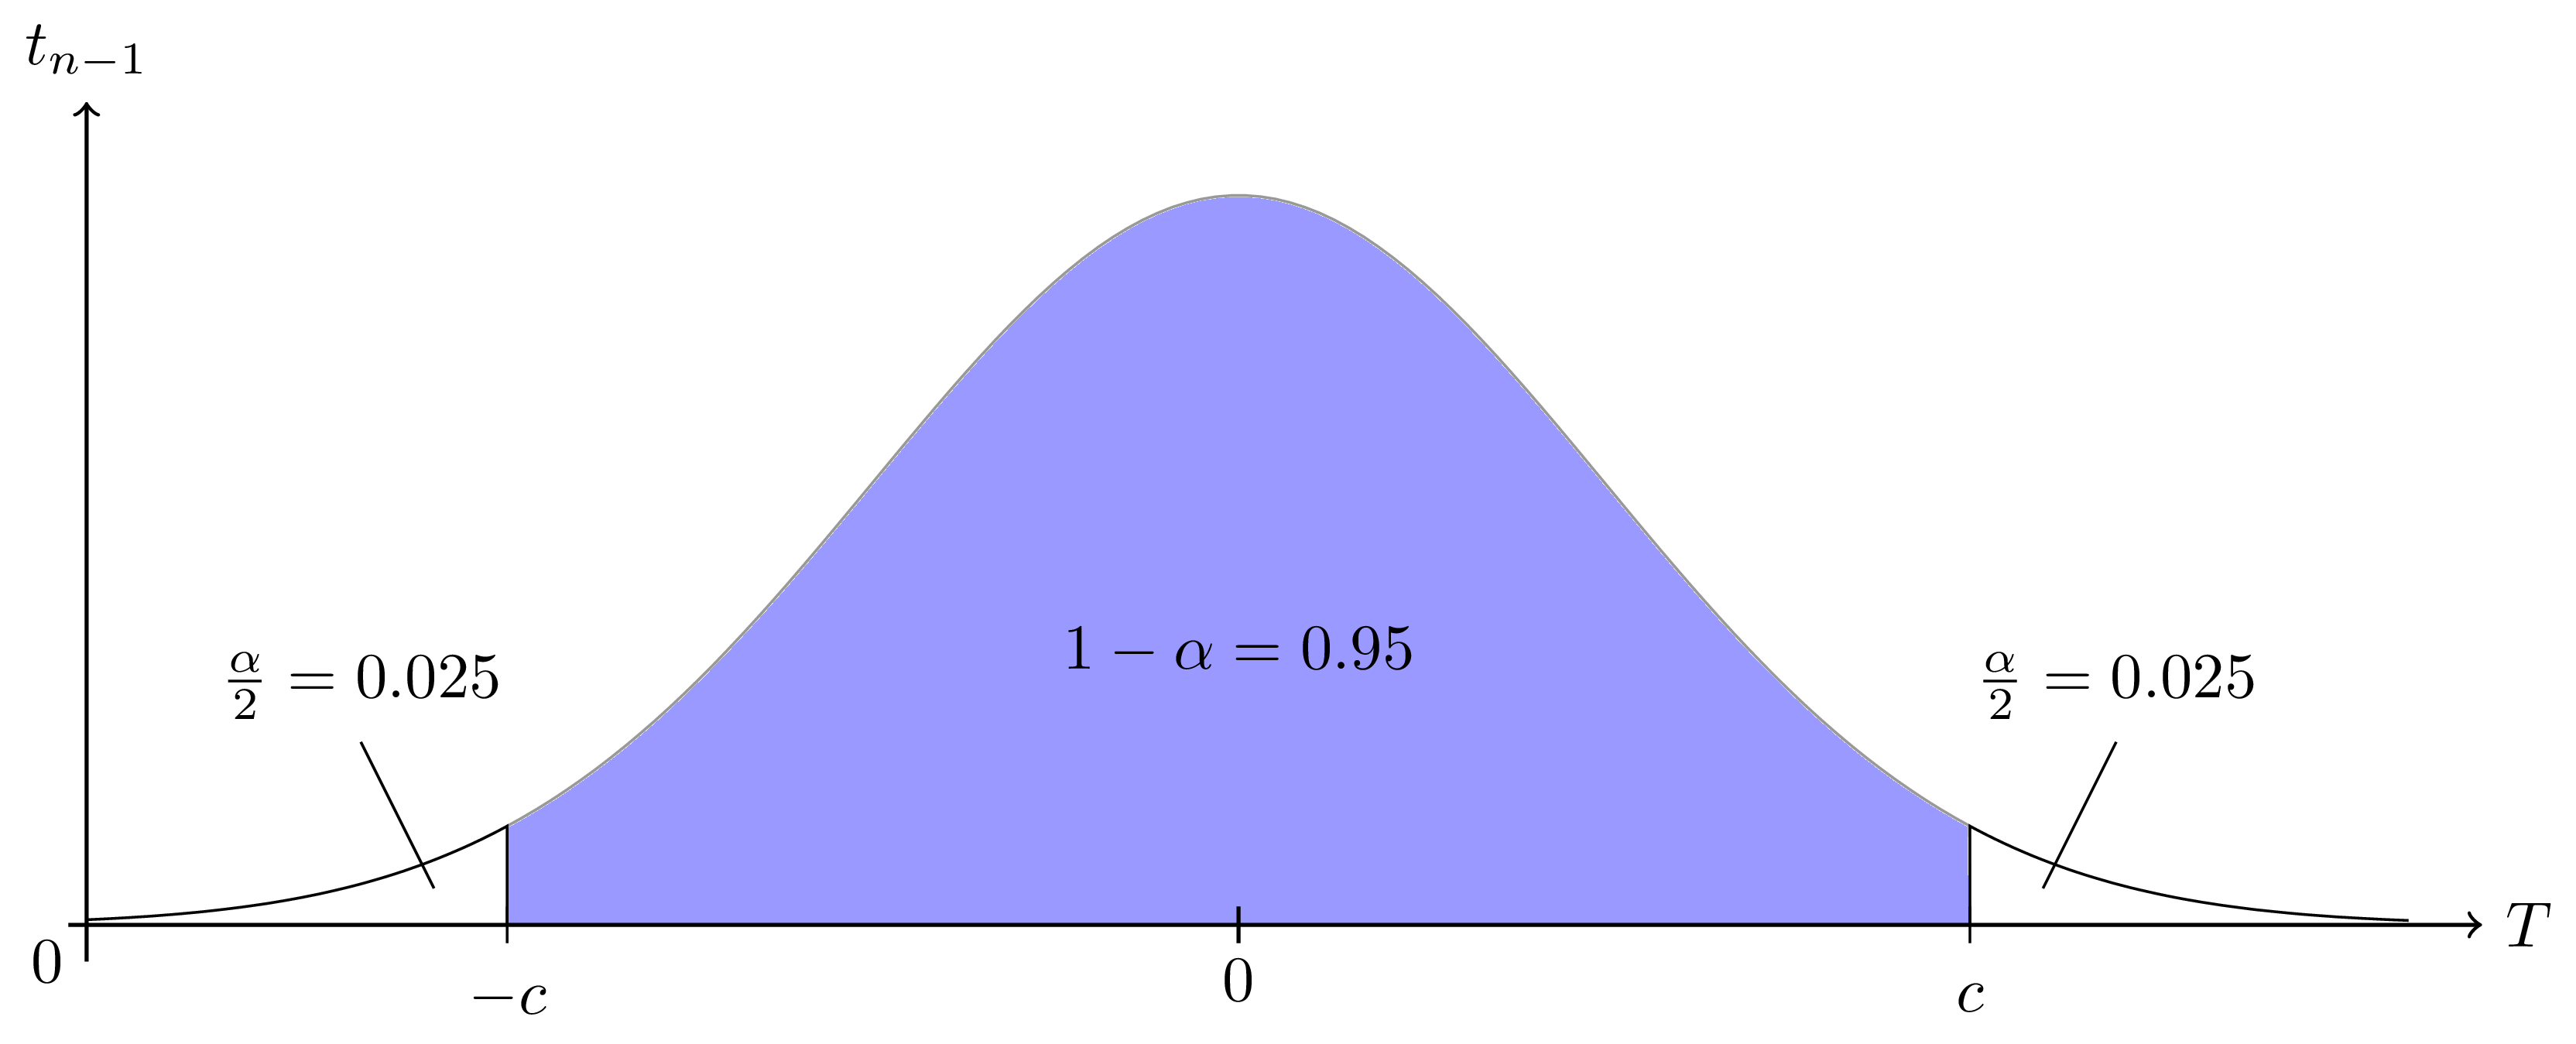
\includegraphics[width=0.9\linewidth]{ScPoEconometrics_files/figure-latex/cifig-1} 

}

\caption{Confidence Interval Construction. The blue area is called *coverage region* which contains the true $\mu$ with probability $1-\alpha$.}\label{fig:cifig}
\end{figure}

Given the symmetry of the \emph{t} distribution it's enough to find
\(c\) at the upper tail: the point above which \(\frac{\alpha}{2}\) of
all probability mass of the \(t_{df}\) distribution comes to lie. In
other words, if \(\mathcal{T}_{df}\) is the CDF of the \emph{t}
distribution with \emph{df} degrees of freedom, we find \(c\) as

\begin{align}
\mathcal{T}_{df}(c)\equiv& \Pr \left( T < c \right)  = 1-\frac{\alpha}{2} = 0.975 \\\label{eq:ci1}
c =& \mathcal{T}_{df}^{-1}(\mathcal{T}_{df}(c)) = \mathcal{T}_{df}^{-1}(0.975)
\end{align}

Here \(\mathcal{T}_{df}^{-1}\) stands for the \emph{quantile function},
i.e.~the inverse of the CDF. In our example with \(df = 49\), you can
find thus that \(c = 2.01\) by typing \texttt{qt(0.975,df=49)} into your
\texttt{R} session.\footnote{You often will see \(c=1.96\), which comes
  from the fact that one relies on the \emph{t} distribution converging
  to the normal distribution with large \(n\). Type
  \texttt{qnorm(0.975)} to confirm!} Now we only have to expand the
definition of the \emph{T} statistic from \eqref{eq:tscore} inside
\eqref{eq:ci} to obtain

\begin{align}
0.95 = 1-\alpha &= \Pr \left(-c \leq T \leq c \right) \\\label{eq:ci2}
                &= \Pr \left(-2.01 \leq \sqrt{n} \frac{\bar{x} - \mu}{s} \leq 2.01 \right) \\
                 &= \Pr \left(\bar{x} -2.01 \frac{s}{\sqrt{n}} \leq \mu \leq \bar{x} + 2.01 \frac{s}{\sqrt{n}} \right) 
\end{align}

Finally, filling in our numbers for \(s\) etc, this implies that a 95\%
confidence interval about the location of the true average height of all
SciencesPo students, \(\mu\), is given by:

\begin{equation}
CI = \left[165.658 , 171.342 \right]
\end{equation}

We would tell the director that with 95\% probability, the true average
height of all students comes to lie within those two bounds.

Finally, looking back at figure \ref{fig:confint} above, the shaded area
is just the 95\% confidence interval \emph{about the true value
\(\beta_1\)}. We would say that \emph{the true regression line} is
contained within the shaded region with 95\% probability. Very similarly
to our example of \(\bar{x}\), in that picture we have instead an
estimate \(b_1\), with an associated standard error \(SE(b_1)\). The
shaded area is called \emph{confidence band}, and it is just plotting
the confidence interval \emph{for each value \(x\)} in the data. You can
see how the band becomes narrower (i.e.~the estimate becomes more
precise) if there is more data associated to a certain \(x\).

\section{Hypothesis Testing}\label{hypothesis-testing}

Now know by now how the standard errors of an OLS estimate are computed,
and what they stand for. We can now briefly\footnote{We will not go into
  great detail here. Please refer back to your statistics course from
  last spring semester (chapters 8 and 9), or the short note I
  \href{images/hypothesis.pdf}{wrote while ago}} discuss a very common
usage of this information, in relation to which variables we should
include in our regression. There is a statistical proceedure called
\emph{hypothesis testing} which helps us to make such decisions. In
\href{https://en.wikipedia.org/wiki/Statistical_hypothesis_testing}{hypothesis
testing}, we have a baseline, or \emph{null} hypothesis \(H_0\), which
we want to confront with a competing \emph{alternative} hypthesis
\(H_1\). Continuing with our example of the mean height of SciencesPo
students (\(\mu\)), one potential hypothesis could be

\begin{align}
H_0:& \mu = 167\\
H_1:& \mu \neq 167
\end{align}

Here we state that under the null hypthesis, \(\mu = 167\), and under
the alternative, it's not equal to that value. This would be called a
\emph{two-sided} test, because it tests deviations from \(H_0\) below as
well as above. An alternative formulation could use the \emph{one-sided}
test that

\begin{align}
H_0:& \mu = 167\\
H_1:& \mu > 167.
\end{align}

which would mean: under the null hypothesis, the average of all ScPo
students' body height is 167cm. Under the alternative, it is larger. You
can immediately see that this is very similar to confidence interval
construction.

Suppose as above that we found \(\bar{x} = 168.5\), and that the sample
standard deviation is still \(s=10\). Would you regard this as strong or
weak evidence against \(H_0\) and in favor of \(H_1\)?

You should now remember what you saw when you did
\texttt{launchApp("estimate")}. Look again at this app and set the
slider to a sample size of \(50\), just as in our running example. You
can see that the app draws one hundred (100) samples for you, locates
their sample mean on the x-axis, and estimates the red density.

\begin{note}
The crucial thing to note here is that, given we are working with a
\textbf{random sample} from a population with a certain distribution of
\emph{height}, our sample statistic \(\bar{x}\) is \textbf{also a random
variable}. Every new set of randomly drawn students would yield a
different \(\bar{x}\), and all of them together would follow the red
density in the app. In reality we often only get to draw one single
sample, and we can use knowledge about the sampling distribution to make
inference.
\end{note}

Our task is now to decide if given that particular sampling
distribution, given our estimate \(\bar{x}\) and given an observed
sample variance \(s^2\), whether \(\bar{x} = 168.5\) is \emph{far away}
from \(\bar{x} = 167\), or not. The way to proceed is by computing a
\emph{test statistic}, which is to be compared to a \emph{critical
value}: if the test statistic exceeds that value, we reject \(H_0\),
otherwise we cannot. The critical value depends on the sampling
distribution, and the size of the test. We talk about this next.

\subsection{Making Errors}\label{making-errors}

There are two types of error one can make when deploying such a test:

\begin{enumerate}
\def\labelenumi{\arabic{enumi}.}
\tightlist
\item
  We might reject \(H_0\), when in fact it is true! Here, upon observing
  \(\bar{x} = 168.5\) we might conclude that indeed \(\mu > 167\) and
  thus we'd reject. But we might have gotten unlucky and by chance have
  obtained an unusually tall sample of students. This is called
  \textbf{type one error}.
\item
  We might \emph{fail} to reject \(H_0\) when in fact \(H_1\) is true.
  This is called the \textbf{type two error}.
\end{enumerate}

We design a test with a certain probability of \emph{type one error}
\(\alpha\) in mind. In other words, we choose with which probability
\(\alpha\) we are willing to make a type one error. (Notice that the
best tests also avoid making type two errors! The number
\(1-\Pr(\text{type 2 error})\) is called \emph{power}, hence we prefer
tests with \emph{high power}). A typical choice for \(\alpha\) is 0.05,
i.e.~we are willing to make a type one error with probability 5\%.
\(\alpha\) is commonly called the \textbf{level of significance} or the
\textbf{size} of a test.

\subsection{Performing the Test}\label{performing-the-test}

We can stick to the following cookbook procedure, which is illustrated
in figure \ref{fig:testfig}.

\begin{enumerate}
\def\labelenumi{\arabic{enumi}.}
\tightlist
\item
  Set up hypothesis and significance level:

  \begin{enumerate}
  \def\labelenumii{\arabic{enumii}.}
  \tightlist
  \item
    \(H_0: \mu = 167\)
  \item
    \(H_1: \mu > 167\)
  \item
    \(\alpha = 0.05\)
  \end{enumerate}
\item
  Test Statistic and test distribution:

  \begin{itemize}
  \tightlist
  \item
    We don't know the true population variance \(\sigma^2\), hence we
    estimate it via \(s^2\) from our sample.
  \item
    The corresponding test statistic is the \emph{t-statistic}, which
    follows the
    \href{https://en.wikipedia.org/wiki/Student's_t-distribution}{Student's
    T} distribution.
  \item
    That is, our statistic is
    \(T=\frac{\bar{x} - \mu}{s/\sqrt{n}} \sim t_{49}\), where 49 is
    equal to the \emph{degrees of freedom} in this case.
  \end{itemize}
\item
  Rejection Region: We perform a one-sided test. We said we are happy
  with a 5\% significance level, i.e.~we are looking for the \(t\) value
  which corresponds \emph{just} to \(1-0.05 = 0.95\) mass under the pdf
  of the \(t\) distribution. More precisely, we are looking for the
  \(1-0.05 = 0.95\) quantile of the \(t_{50}\) distribution.\footnote{See
    the previous footnote for an explanation of this!} This implies a
  critical value \(c = 1.676\), which you can verify by typing
  \texttt{qt(0.95,df=50)} in \texttt{R}.
\item
  Calculate our test statistic:
  \(\frac{\bar{x} - \mu}{s/\sqrt{n}} = \frac{168.5 - 167}{20/\sqrt{50}} = 1.061\)
\item
  Decide: We find that \(1.061 < 1.676\). Hence, we cannot reject
  \(H_0\), because we only found weak evidence against it in our sample
  of data.
\end{enumerate}

\begin{figure}

{\centering 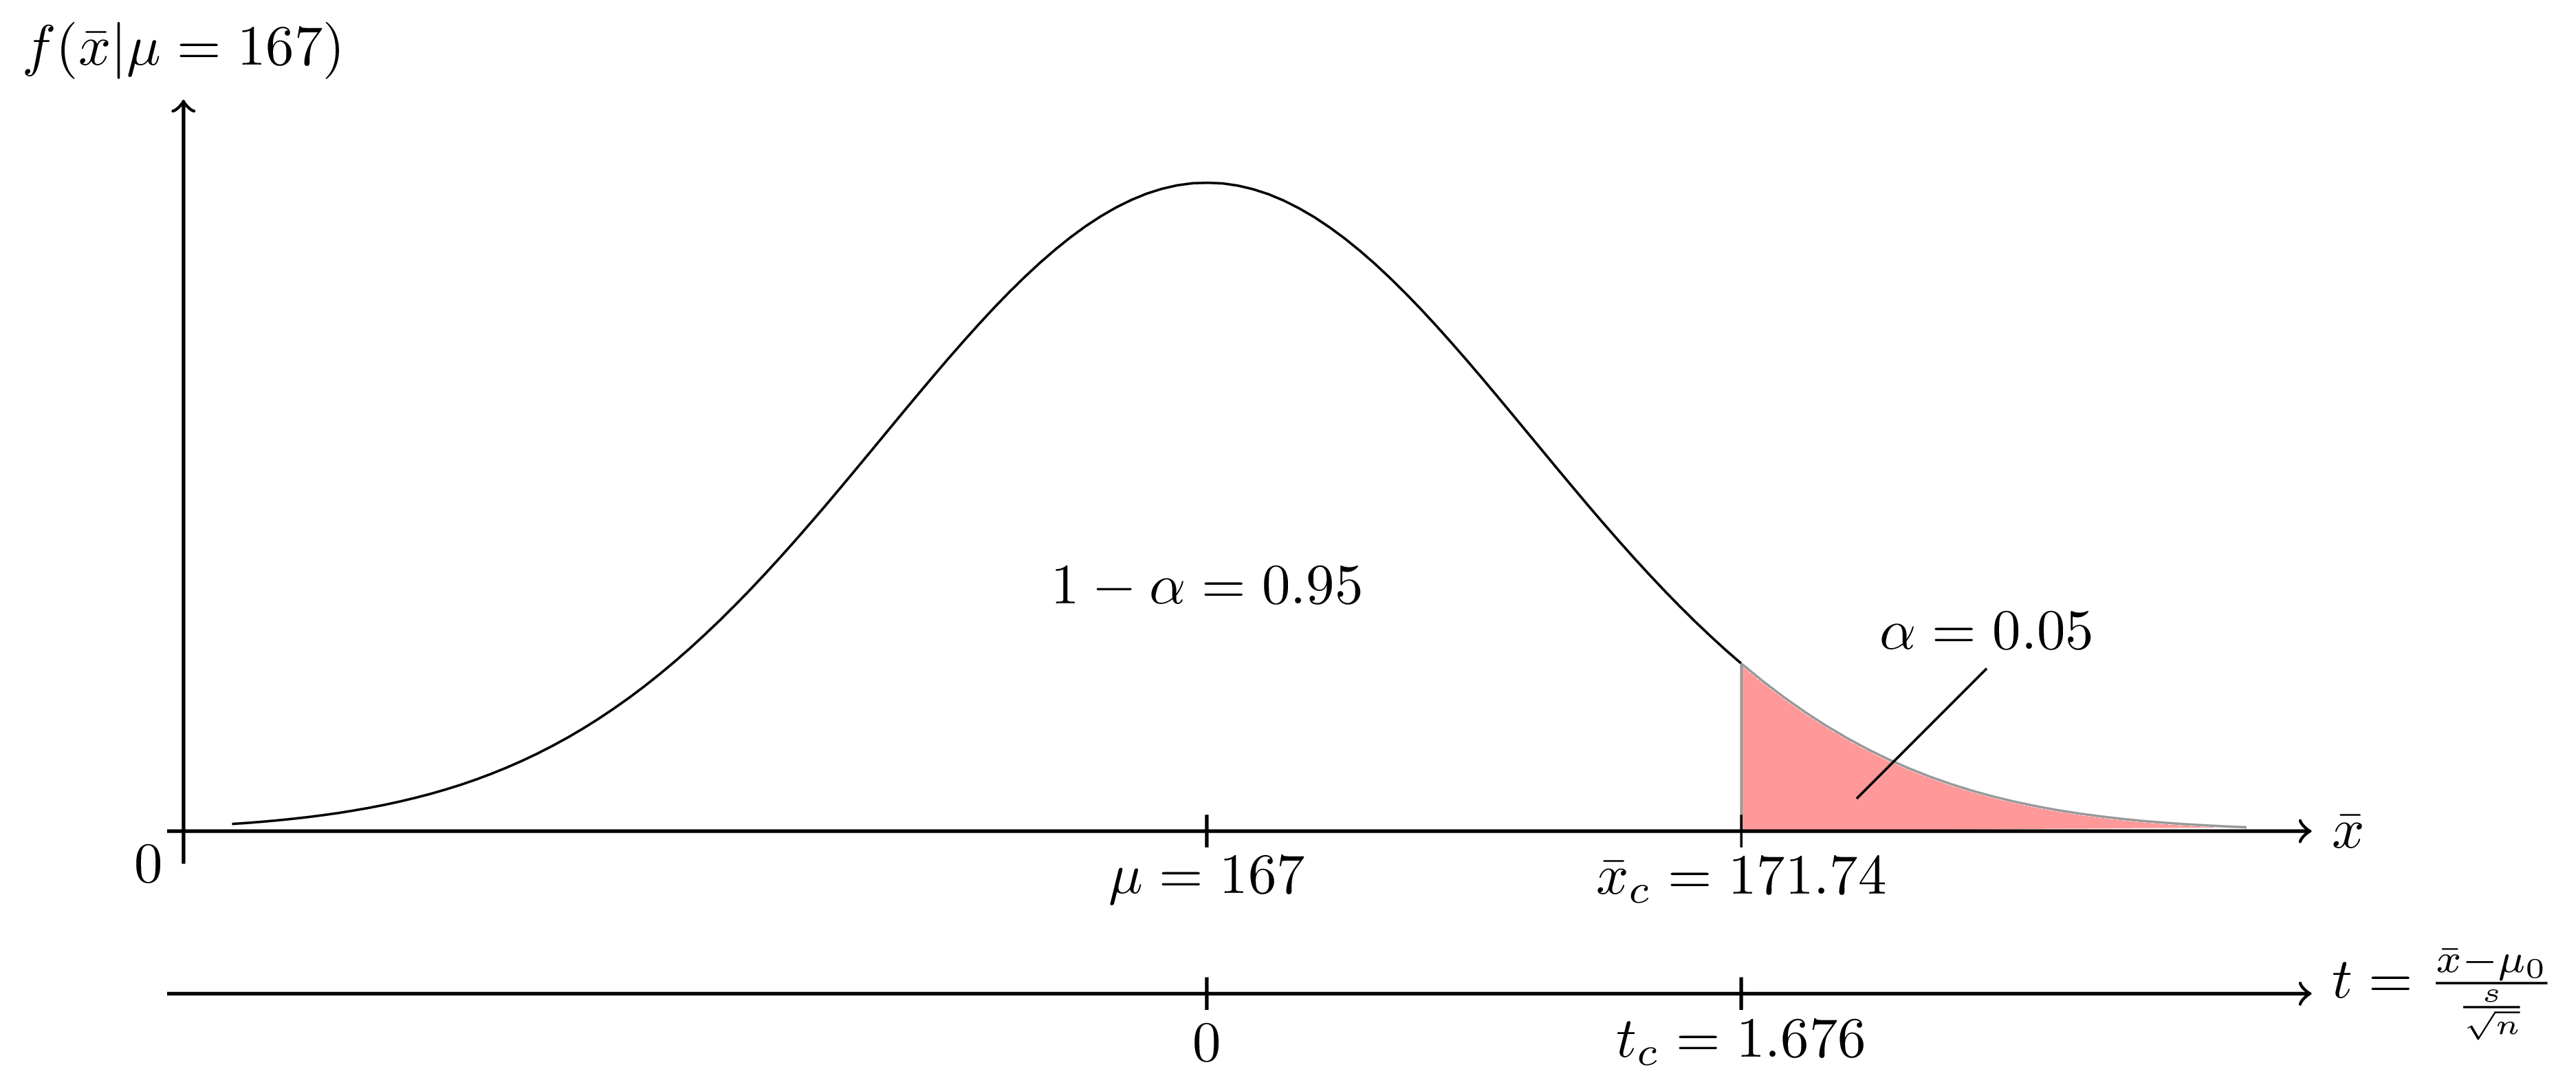
\includegraphics[width=0.9\linewidth]{ScPoEconometrics_files/figure-latex/testfig-1} 

}

\caption{Cookbook Testing Proceedure. Subscripts $c$ indicate *critical value*. There are two x-axis: one for values of $\bar{x}$, and one for the corresponding $t$ statistic. The red area is the rejection area. If we observe a test statistic such that $t>t_c$, we feel reassured that our $\bar{x}$ is *sufficiently far away* from the hypothesized value $\mu$, such that we feel comfortable with rejecting $H_0$. And vice versa: If our test statistic falls below $t_c$, we will not reject $H_0$}\label{fig:testfig}
\end{figure}

\subsection{Testing Regression
Coefficients}\label{testing-regression-coefficients}

In Regression Analysis, we often want to test a very specific
alternative hypothesis: We want to have a quick way to tell us whether a
certain variable \(x_k\) is \emph{relevant} in our statistical model or
not. In hypothesis testing language, that would be

\begin{align}
H_0:& \beta_k = 0\\
H_1:& \beta_k \neq 0.\label{eq:H0}
\end{align}

Clearly, if in the \textbf{true} regression model we find \(\beta_k=0\),
this means that \(x_k\) has a zero partial effect on the outcome, hence
it should be excluded from the regression. Notice that we are interested
in \(\beta_k\), not in \(b_k\), which is the estimator that we compute
from our sample (similarly to \(\bar{x}\), which estimates \(\mu\)
above).

As such, this is a \emph{two-sided test}. We can again illustrate this
in figure \ref{fig:testfig2}. Notice how we now have two rejection
areas.

\begin{figure}

{\centering 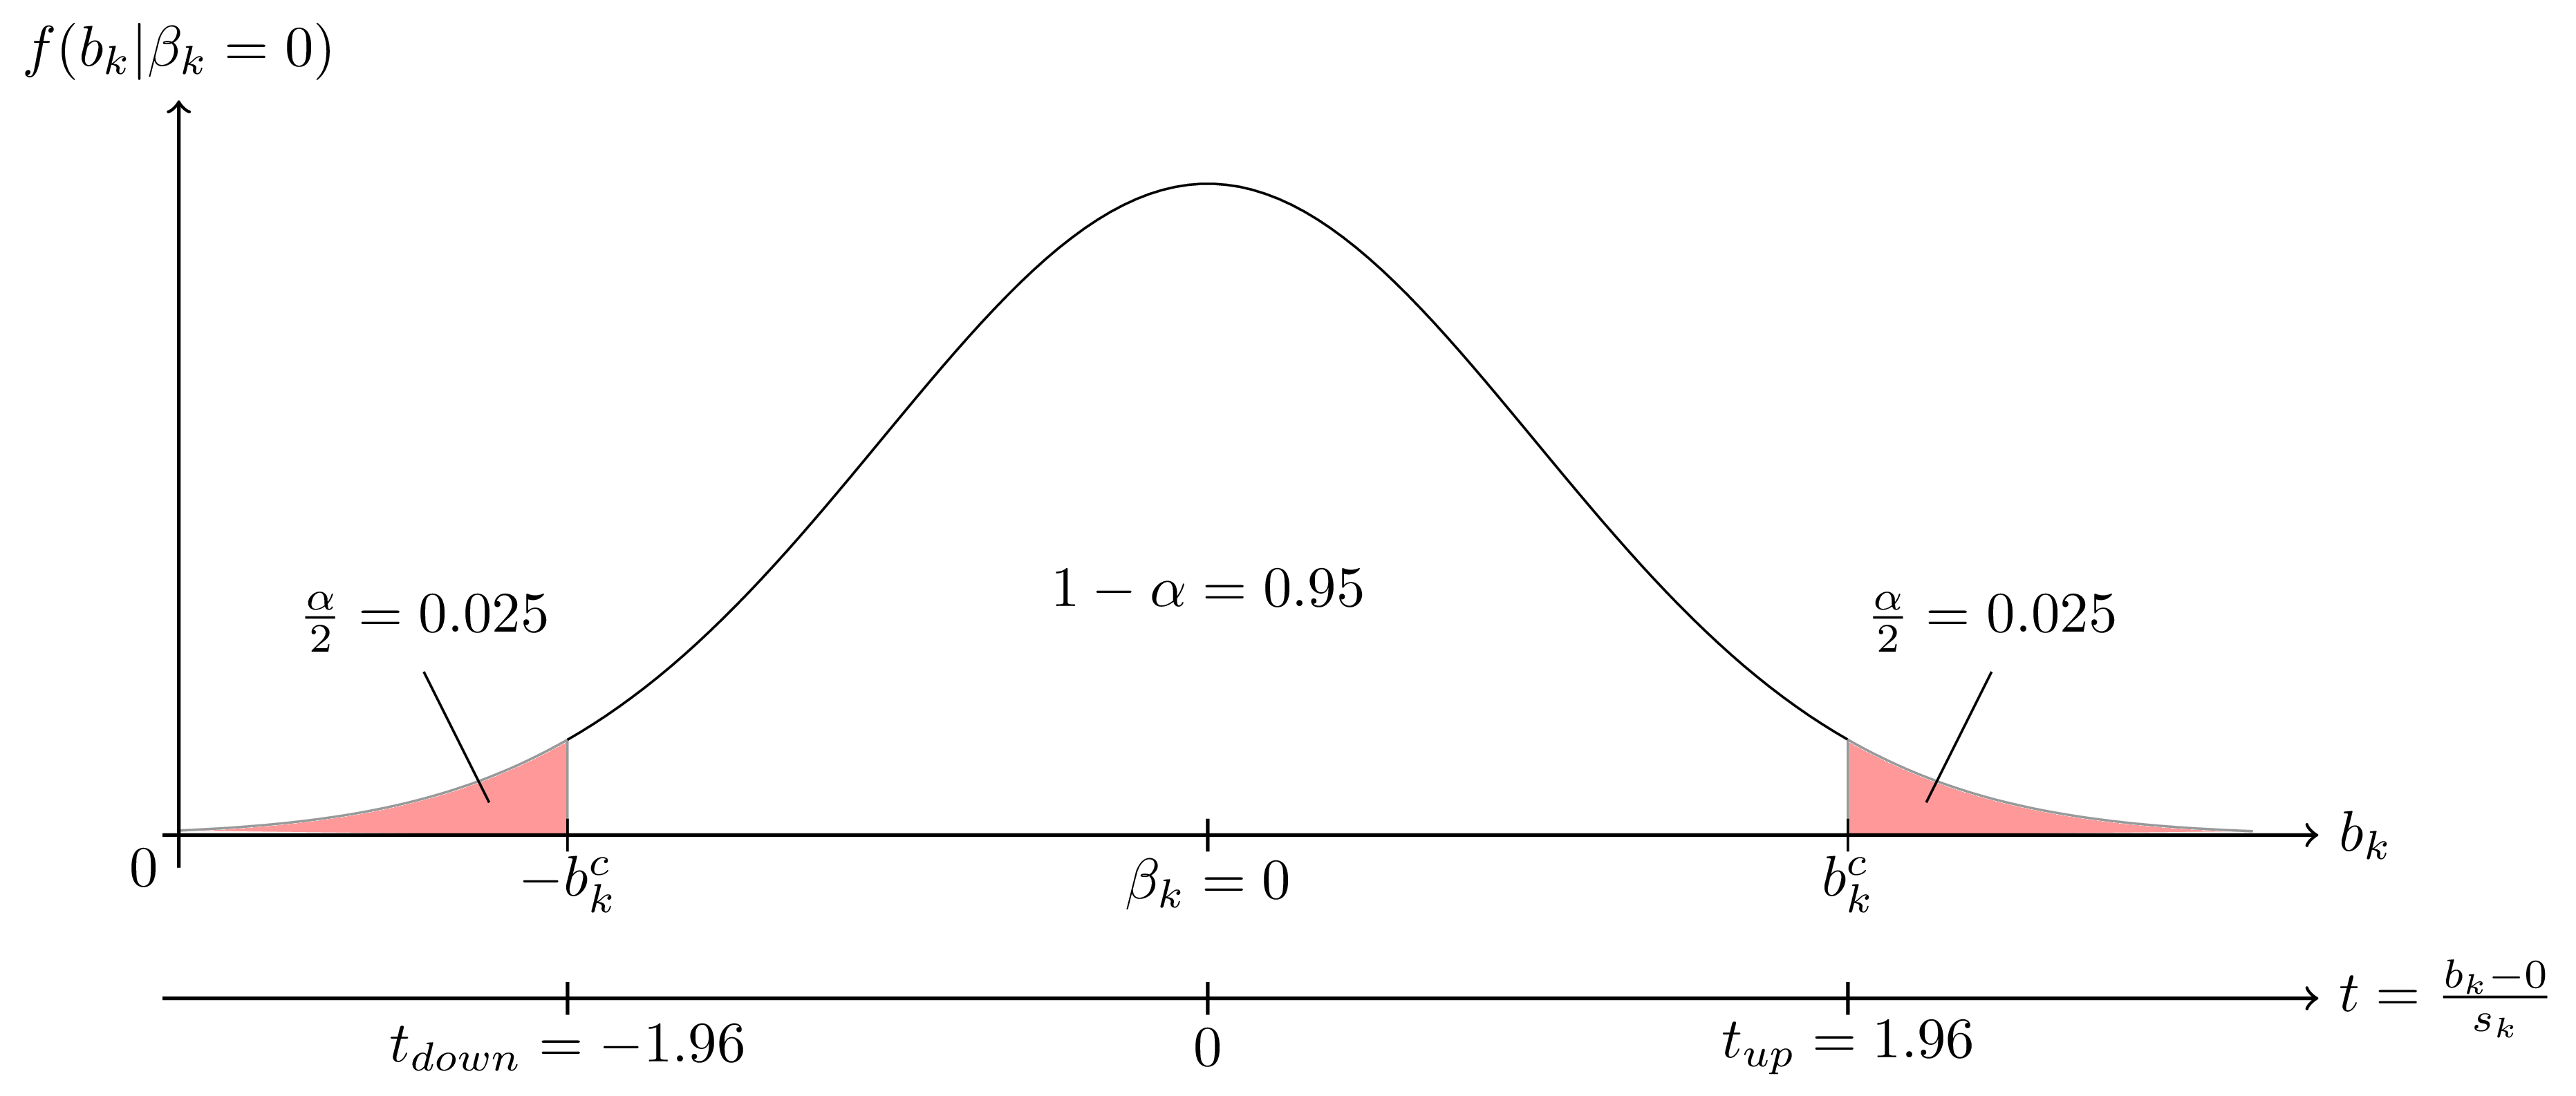
\includegraphics[width=0.9\linewidth]{ScPoEconometrics_files/figure-latex/testfig2-1} 

}

\caption{Testing whether coefficient $b_k$ is *statistically significantly different* from zero. Now we have two red rejection areas. We relabel critical values with a superscript here. If we observe a test statistic falling in either red region, we reject, else we do not. Notice that the true value under $H_0$ is $\beta_k=0$. }\label{fig:testfig2}
\end{figure}

The relevant test statistic for a regression coefficient is again the
\emph{t} distribution. In fact, this particular test is so important
that all statistical packages report the \emph{t} statistic
corresponding to \eqref{eq:H0} automatically. Let's look at an example:

\begin{verbatim}
#OUT> 
#OUT> Call:
#OUT> lm(formula = mpg ~ wt + hp + drat, data = mtcars)
#OUT> 
#OUT> Residuals:
#OUT>     Min      1Q  Median      3Q     Max 
#OUT> -3.3598 -1.8374 -0.5099  0.9681  5.7078 
#OUT> 
#OUT> Coefficients:
#OUT>              Estimate Std. Error t value Pr(>|t|)    
#OUT> (Intercept) 29.394934   6.156303   4.775 5.13e-05 ***
#OUT> wt          -3.227954   0.796398  -4.053 0.000364 ***
#OUT> hp          -0.032230   0.008925  -3.611 0.001178 ** 
#OUT> drat         1.615049   1.226983   1.316 0.198755    
#OUT> ---
#OUT> Signif. codes:  0 '***' 0.001 '**' 0.01 '*' 0.05 '.' 0.1 ' ' 1
#OUT> 
#OUT> Residual standard error: 2.561 on 28 degrees of freedom
#OUT> Multiple R-squared:  0.8369,  Adjusted R-squared:  0.8194 
#OUT> F-statistic: 47.88 on 3 and 28 DF,  p-value: 3.768e-11
\end{verbatim}

The column \texttt{t\ value} is just \texttt{Estimate} divided by
\texttt{Std.\ Error}. That is, \texttt{R} reports in the column
\texttt{t\ value} the following number for us:

\begin{equation}
\text{t value} = \frac{b_k-0}{s_k}  \label{eq:tstat}
\end{equation}

where \(s_k\) is the estimated standard error as introduced in
\ref{se-theory}, and where we test \(H_0:\beta_k = 0\). Notice that this
particular \emph{t} statistic is different from our previous formulation
in \eqref{eq:tscore}: we don't have to scale by \(\sqrt{n}\)! This is so
because \texttt{R} and other statistical software assumes the
\emph{normal} linear regression model (see \ref{class-reg}). Normality
of the regression error \(\varepsilon\) implies that the \emph{t}
statistic looks like in \eqref{eq:tstat}.

We have to choose a critical value for this test. Many people
automatically choose the 0.975 quantile of the standard normal
distribution, \texttt{qnorm(0.975)}, 1.96 in this case. This is fine for
sample sizes greater than 100, say. In this regression, we only have 28
degrees of freedom, so we better choose the critical value from the
\emph{t} distribution as above. We get \(t_{down} = -2.048\) and
\(t_{up} = 2.048\) as critical values. Let's test whether the
coefficient on \texttt{wt} is statistically different from zero:

\begin{align}
H_0:& \beta_{wt} = 0\\
H_1:& \beta_{wt} \neq 0 \label{eq:mtcarswt}
\end{align}

We just take the \texttt{t\ value} entry, and see whether it lies above
or below either critical value: Indeed, we see that \(-4.053 < -2.048\),
and we are happy to reject \(H_0\).

On the other hand, when testing for statistical significance of
\texttt{drat} that does not seem to be the case:

\begin{align}
H_0:& \beta_{drat} = 0\\
H_1:& \beta_{drat} \neq 0 \label{eq:mtcarsdrat}
\end{align}

Here we find that \(1.316 \in [-2.048,2.048]\), hence it does not lie in
any rejection region, and we can \emph{not} reject \(H_0\). We would say
that \emph{coefficient \(\beta_{drat}\) is not statistically significant
at the 5\% level}. As such, we should not include it in our regression.

\subsection{P-Values and Stars}\label{p-values-and-stars}

\texttt{R} also reports two additional columns in its regression output.
The so-called \emph{p-value} in column
\texttt{Pr(\textgreater{}\textbar{}t\textbar{})} and a column with
stars. P-values are an improvement over the dichotomy introduced in the
standard reject/accept framework above. We never know if we
\emph{narrowly} rejected a \(H_0\), or not. The p-value is defined as
the particular level of significance \(\alpha^*\), up to which
\emph{all} \(H_0\)'s would be rejected. If this is a very small number,
we have overwhelming support to reject the null. If, on the contrary,
\(\alpha^*\) turns out to be rather large, we only found weak evidence
against \(H_0\).

We define the p-value as the sum of rejection areas for a given test
statistic \(T^*\). Notice that the symmetry of the \(t\) distribution
implies that we multiply by two each of the two tail probabilities:

\begin{align}
\alpha^* = 2 \Pr(t > |T^*|) 
\end{align}

The stars in the final column are a visualization of this information.
They show a quick summary of the magnitude of each p-value. Commonly,
\texttt{***} means an extremely small reference significance level
\(\alpha^*=0\) (almost zero), \texttt{**} means \(\alpha^*=0.001\), etc.
In that case, up to a significance level of 0.1\%, all \(H_0\) would be
rejected. You clearly see that all columns \texttt{Std.\ Error},
\texttt{t\ value} and \texttt{Pr(\textgreater{}\textbar{}t\textbar{})}
give a different type of the same information.

\section{What's in my model? (And what is
not?)}\label{whats-in-my-model-and-what-is-not}

We want to revisit the underlying assumptions of the classical model
outlined in \ref{class-reg}. Right now we to talk a bit more about
assumption number 2 of the above definition in \ref{class-reg}. It said
this:

\begin{warning}
The mean of the residuals conditional on \(x\) should be zero,
\(E[\varepsilon|x] = 0\). This means that \(Cov(\varepsilon,x) = 0\),
i.e.~that the errors and our explanatory variable(s) should be
\emph{uncorrelated}. We want \(x\) to be \textbf{strictly exogenous} to
the model.
\end{warning}

 Great. But what does this \emph{mean}? How could \(x\) be correlated
with something we don't even observe?! Good questions - let's try with
an example.

Imagine that we assume that

\begin{equation}
y_i = \beta_0 + \beta_1 x_i + \varepsilon_i \label{eq:DGP-h}
\end{equation}

represents the DGP of impact the sales price of houses (\(y\)) as a
function of number of bathrooms (\(x\)). We run OLS as

\[
y_i = b_0 + b_1 x_i + e_i 
\] You find a positive impact of bathrooms on houses:

\begin{verbatim}
#OUT> 
#OUT> Call:
#OUT> lm(formula = price ~ bathrms, data = Housing)
#OUT> 
#OUT> Residuals:
#OUT>    Min     1Q Median     3Q    Max 
#OUT> -77225 -15271  -2510  11704 102729 
#OUT> 
#OUT> Coefficients:
#OUT>             Estimate Std. Error t value Pr(>|t|)    
#OUT> (Intercept)    32794       2694   12.17   <2e-16 ***
#OUT> bathrms        27477       1952   14.08   <2e-16 ***
#OUT> ---
#OUT> Signif. codes:  0 '***' 0.001 '**' 0.01 '*' 0.05 '.' 0.1 ' ' 1
#OUT> 
#OUT> Residual standard error: 22880 on 544 degrees of freedom
#OUT> Multiple R-squared:  0.267,   Adjusted R-squared:  0.2657 
#OUT> F-statistic: 198.2 on 1 and 544 DF,  p-value: < 2.2e-16
\end{verbatim}

In fact, from this you conclude that each additional bathroom increases
the sales price of a house by 27477 dollars. Let's see if our assumption
\(E[\varepsilon|x] = 0\) is satisfied:

\begin{Shaded}
\begin{Highlighting}[]
\KeywordTok{library}\NormalTok{(dplyr)}
\CommentTok{# add residuals to the data}
\NormalTok{Housing}\OperatorTok{$}\NormalTok{resid <-}\StringTok{ }\KeywordTok{resid}\NormalTok{(hlm)}
\NormalTok{Housing }\OperatorTok
\StringTok{  }\KeywordTok{group_by}\NormalTok{(bathrms) }\OperatorTok
\StringTok{  }\KeywordTok{summarise}\NormalTok{(}\DataTypeTok{mean_of_resid=}\KeywordTok{mean}\NormalTok{(resid))}
\end{Highlighting}
\end{Shaded}

\begin{verbatim}
#OUT> # A tibble: 4 x 2
#OUT>   bathrms mean_of_resid
#OUT>     <dbl>         <dbl>
#OUT> 1       1         -118.
#OUT> 2       2          955.
#OUT> 3       3       -11195.
#OUT> 4       4        32298.
\end{verbatim}

Oh, that doesn't look good. Even though the unconditional mean
\(E[e] = 0\) is \emph{very} close to zero (type
\texttt{mean(resid(hlm))}!), this doesn't seem to hold at all by
categories of \(x\). This indicates that there is something in the error
term \(e\) which is \emph{correlated} with \texttt{bathrms}. Going back
to our discussion about \emph{ceteris paribus} in section \ref{ceteris},
we stated that the interpretation of our OLS slope estimate is that

\begin{tip}
Keeping everything else fixed at the current value, what is the impact
of \(x\) on \(y\)? \emph{Everything} also includes things in
\(\varepsilon\) (and, hence, \(e\))!
\end{tip}

 It looks like our DGP in \eqref{eq:DGP-h} is the \emph{wrong model}.
Suppose instead, that in reality sales prices are generated like this:

\begin{equation}
y_i = \beta_0 + \beta_1 x_i + \beta_2 z_i + \varepsilon_i \label{eq:DGP-h2}
\end{equation}

This would now mean that by running our regression, informed by the
wrong DGP, what we estimate is in fact this: \[
y_i = b_0 + b_1 x_i + (b_2 z_i + e_i)  = b_0 + b_1 x_i + u_i.
\] This is to say that by \emph{omitting} variable \(z\), we relegate it
to a new error term, here called \(u_i = b_2 z_i + e_i\). Our assumption
above states that \emph{all regressors need to be uncorrelated with the
error term} - so, if \(Corr(x,z)\neq 0\), we have a problem. Let's take
this idea to our running example.

\subsection{Omitted Variable Bias}\label{omitted-variable-bias}

What we are discussing here is called \emph{Omitted Variable Bias}.
There is a variable which we omitted from our regression, i.e.~we forgot
to include it. It is often difficult to find out what that variable
could be, and you can go a long way by just reasoning about the
data-generating process. In other words, do you think it's
\emph{reasonable} that price be determined by the number of bathrooms
only? Or could there be another variable, omitted from our model, that
is important to explain prices, and at the same time correlated with
\texttt{bathrms}?

Let's try with \texttt{lotsize}, i.e.~the size of the area on which the
house stands. Intuitively, larger lots should command a higher price; At
the same time, however, larger lots imply more space, hence, you can
also have more bathrooms! Let's check this out:

\begin{verbatim}
#OUT> 
#OUT> Call:
#OUT> lm(formula = price ~ bathrms + lotsize, data = Housing)
#OUT> 
#OUT> Residuals:
#OUT>    Min     1Q Median     3Q    Max 
#OUT> -60752 -12532  -1674  10514  92931 
#OUT> 
#OUT> Coefficients:
#OUT>              Estimate Std. Error t value Pr(>|t|)    
#OUT> (Intercept) 1.008e+04  2.810e+03   3.588 0.000364 ***
#OUT> bathrms     2.281e+04  1.703e+03  13.397  < 2e-16 ***
#OUT> lotsize     5.575e+00  3.944e-01  14.136  < 2e-16 ***
#OUT> ---
#OUT> Signif. codes:  0 '***' 0.001 '**' 0.01 '*' 0.05 '.' 0.1 ' ' 1
#OUT> 
#OUT> Residual standard error: 19580 on 543 degrees of freedom
#OUT> Multiple R-squared:  0.4642,  Adjusted R-squared:  0.4622 
#OUT> F-statistic: 235.2 on 2 and 543 DF,  p-value: < 2.2e-16
\end{verbatim}

Here we see that the estimate for the effect of an additional bathroom
\emph{decreased} from 27477 to 22811.5 by almost 5000 dollars! Well
that's the problem then. We said above that one more bathroom is worth
27477 dollars - if \textbf{nothing else changes}! But that doesn't seem
to hold, because we have seen that as we increase \texttt{bathrms} from
\texttt{1} to \texttt{2}, the mean of the resulting residuals changes
quite a bit. So there \textbf{is something in \(\varepsilon\) which does
change}, hence, our conclusion that one more bathroom is worth 27477
dollars is in fact \emph{invalid}!

The way in which \texttt{bathrms} and \texttt{lotsize} are correlated is
important here, so let's investigate that:

\begin{figure}

{\centering 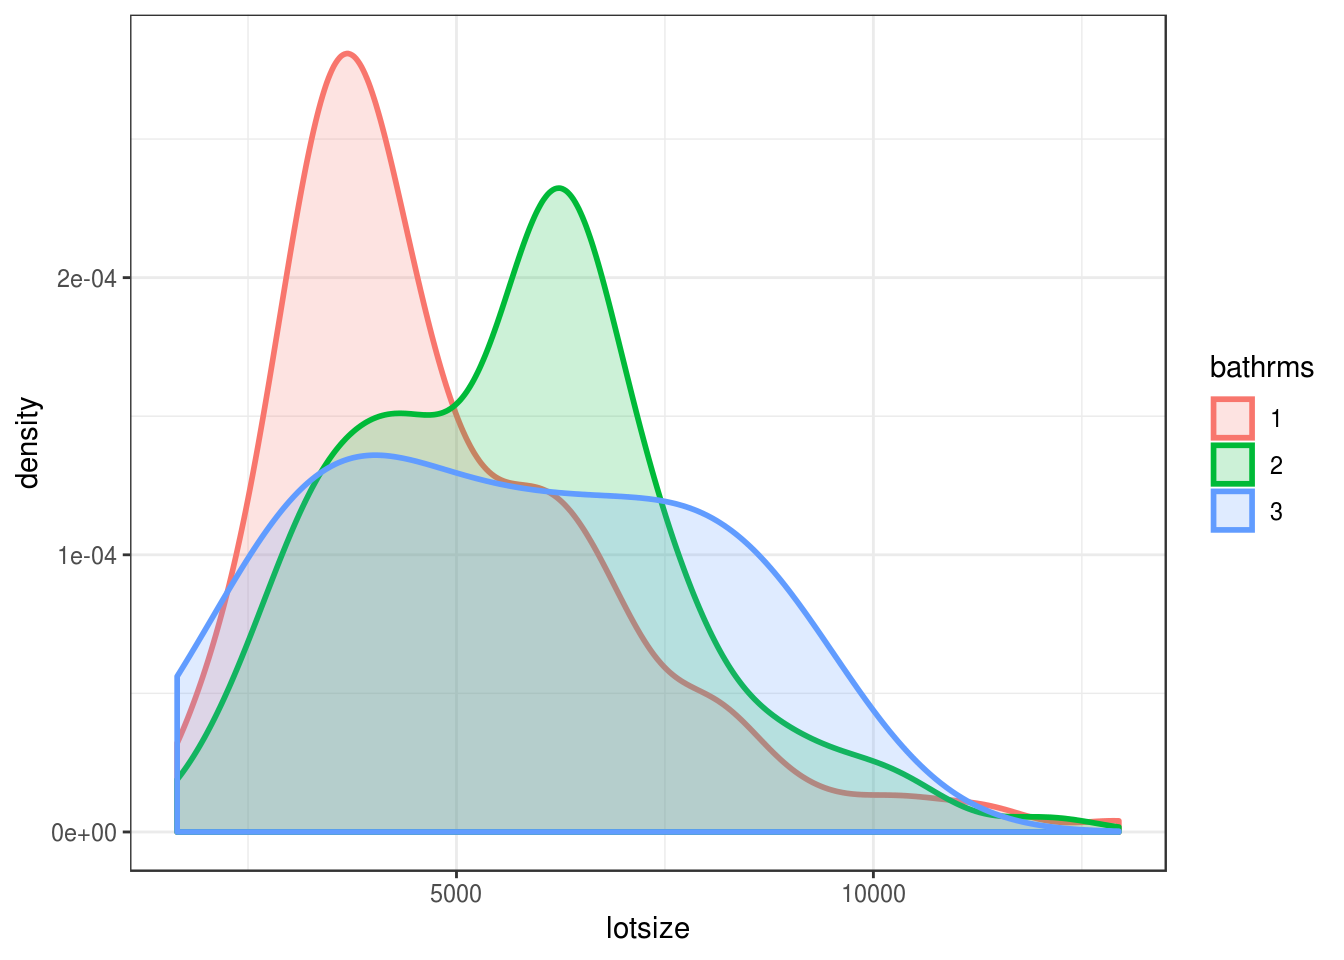
\includegraphics{ScPoEconometrics_files/figure-latex/unnamed-chunk-159-1} 

}

\caption{Distribution of `lotsize` by `bathrms`}\label{fig:unnamed-chunk-159}
\end{figure}

This shows that lotsize and the number of bathrooms is indeed positively
related. Larger lot of the house, more bathrooms. This leads to a
general result:

\begin{note}
\textbf{Direction of Omitted Variable Bias}

If there is an omitted variable \(z\) that is \emph{positively}
correlated with our explanatory variable \(x\), then our estimate of
effect of \(x\) on \(y\) will be too large (or, \emph{biased upwards}).
The correlation between \(x\) and \(z\) means that we attribute part of
the impact of \(z\) on \(y\) mistakenly to \(x\)! And, of course, vice
versa for \emph{negatively} correlated omitted variables.
\end{note}

\chapter{Quantile Regression}\label{quantreg}

\begin{enumerate}
\def\labelenumi{\arabic{enumi}.}
\tightlist
\item
  before you were modelling the mean. the average link
\item
  now what happens to \textbf{outliers}? how robust is the mean to that
\item
  what about the entire distribution of this?
\end{enumerate}

\chapter{Panel Data}\label{panel-data}

\section{fixed effects}\label{fixed-effects}

\section{DiD}\label{did}

\section{RDD}\label{rdd}

\section{Example}\label{example}

\begin{itemize}
\tightlist
\item
  scanner data on breakfast cereals, \((Q_{it},D_{it})\)
\item
  why does D vary with Q
\item
  pos relation ship
\item
  don't observe the group identity!
\item
  unobserved het alpha is correlated with Q
\item
  within group estimator
\item
  what if you don't have panel data?
\end{itemize}

\chapter{Instrumental Variables}\label{IV}

\begin{itemize}
\tightlist
\item
  Measurement error
\item
  Omitted Variable Bias
\item
  Reverse Causality / Simultaneity Bias
\end{itemize}

are all called \emph{endogeneity} problems.

\section{Simultaneity Bias}\label{simultaneity-bias}

\begin{itemize}
\tightlist
\item
  Detroit has a large police force
\item
  Detroit has a high crime rate
\item
  Omaha has a small police force
\item
  Omana has a small crime rate
\end{itemize}

Do large police forces \textbf{cause} high crime rates?

Absurd! Absurd? How could we use data to tell?

We have the problem that large police forces and high crime rates covary
positively in the data, and for obvious reasons: Cities want to protect
their citizens and therefore respond to increased crime with increased
police. Using mathematical symbols, we have the following \emph{system
of linear equations}, i.e.~two equations which are \textbf{jointly
determined}:

\begin{align*}
\text{crime}_{it} &= f(\text{police}_{it}) \\
\text{police}_{it}&= g(\text{crime}_{it} )
\end{align*}

We need a factor that is outside this circular system, affecting
\textbf{only} the size of the police force, but not the actual crime
rate. Such a factor is called an \emph{instrumental variable}.

\chapter{Logit and Probit}\label{logit-probit}

\chapter{Principal Component Analysis}\label{pca}

\chapter{\texorpdfstring{Advanced
\texttt{R}}{Advanced R}}\label{R-advanced}

This chapter continues with some advanced usage examples from chapter
\ref{R-intro}

\section{More Vectorization}\label{more-vectorization}

\begin{Shaded}
\begin{Highlighting}[]
\NormalTok{x =}\StringTok{ }\KeywordTok{c}\NormalTok{(}\DecValTok{1}\NormalTok{, }\DecValTok{3}\NormalTok{, }\DecValTok{5}\NormalTok{, }\DecValTok{7}\NormalTok{, }\DecValTok{8}\NormalTok{, }\DecValTok{9}\NormalTok{)}
\NormalTok{y =}\StringTok{ }\DecValTok{1}\OperatorTok{:}\DecValTok{100}
\end{Highlighting}
\end{Shaded}

\begin{Shaded}
\begin{Highlighting}[]
\NormalTok{x }\OperatorTok{+}\StringTok{ }\DecValTok{2}
\end{Highlighting}
\end{Shaded}

\begin{verbatim}
#OUT> [1]  3  5  7  9 10 11
\end{verbatim}

\begin{Shaded}
\begin{Highlighting}[]
\NormalTok{x }\OperatorTok{+}\StringTok{ }\KeywordTok{rep}\NormalTok{(}\DecValTok{2}\NormalTok{, }\DecValTok{6}\NormalTok{)}
\end{Highlighting}
\end{Shaded}

\begin{verbatim}
#OUT> [1]  3  5  7  9 10 11
\end{verbatim}

\begin{Shaded}
\begin{Highlighting}[]
\NormalTok{x }\OperatorTok{>}\StringTok{ }\DecValTok{3}
\end{Highlighting}
\end{Shaded}

\begin{verbatim}
#OUT> [1] FALSE FALSE  TRUE  TRUE  TRUE  TRUE
\end{verbatim}

\begin{Shaded}
\begin{Highlighting}[]
\NormalTok{x }\OperatorTok{>}\StringTok{ }\KeywordTok{rep}\NormalTok{(}\DecValTok{3}\NormalTok{, }\DecValTok{6}\NormalTok{)}
\end{Highlighting}
\end{Shaded}

\begin{verbatim}
#OUT> [1] FALSE FALSE  TRUE  TRUE  TRUE  TRUE
\end{verbatim}

\begin{Shaded}
\begin{Highlighting}[]
\NormalTok{x }\OperatorTok{+}\StringTok{ }\NormalTok{y}
\end{Highlighting}
\end{Shaded}

\begin{verbatim}
#OUT> Warning in x + y: longer object length is not a multiple of shorter object
#OUT> length
\end{verbatim}

\begin{verbatim}
#OUT>   [1]   2   5   8  11  13  15   8  11  14  17  19  21  14  17  20  23  25
#OUT>  [18]  27  20  23  26  29  31  33  26  29  32  35  37  39  32  35  38  41
#OUT>  [35]  43  45  38  41  44  47  49  51  44  47  50  53  55  57  50  53  56
#OUT>  [52]  59  61  63  56  59  62  65  67  69  62  65  68  71  73  75  68  71
#OUT>  [69]  74  77  79  81  74  77  80  83  85  87  80  83  86  89  91  93  86
#OUT>  [86]  89  92  95  97  99  92  95  98 101 103 105  98 101 104 107
\end{verbatim}

\begin{Shaded}
\begin{Highlighting}[]
\KeywordTok{length}\NormalTok{(x)}
\end{Highlighting}
\end{Shaded}

\begin{verbatim}
#OUT> [1] 6
\end{verbatim}

\begin{Shaded}
\begin{Highlighting}[]
\KeywordTok{length}\NormalTok{(y)}
\end{Highlighting}
\end{Shaded}

\begin{verbatim}
#OUT> [1] 100
\end{verbatim}

\begin{Shaded}
\begin{Highlighting}[]
\KeywordTok{length}\NormalTok{(y) }\OperatorTok{/}\StringTok{ }\KeywordTok{length}\NormalTok{(x)}
\end{Highlighting}
\end{Shaded}

\begin{verbatim}
#OUT> [1] 16.66667
\end{verbatim}

\begin{Shaded}
\begin{Highlighting}[]
\NormalTok{(x }\OperatorTok{+}\StringTok{ }\NormalTok{y) }\OperatorTok{-}\StringTok{ }\NormalTok{y}
\end{Highlighting}
\end{Shaded}

\begin{verbatim}
#OUT> Warning in x + y: longer object length is not a multiple of shorter object
#OUT> length
\end{verbatim}

\begin{verbatim}
#OUT>   [1] 1 3 5 7 8 9 1 3 5 7 8 9 1 3 5 7 8 9 1 3 5 7 8 9 1 3 5 7 8 9 1 3 5 7 8
#OUT>  [36] 9 1 3 5 7 8 9 1 3 5 7 8 9 1 3 5 7 8 9 1 3 5 7 8 9 1 3 5 7 8 9 1 3 5 7
#OUT>  [71] 8 9 1 3 5 7 8 9 1 3 5 7 8 9 1 3 5 7 8 9 1 3 5 7 8 9 1 3 5 7
\end{verbatim}

\begin{Shaded}
\begin{Highlighting}[]
\NormalTok{y =}\StringTok{ }\DecValTok{1}\OperatorTok{:}\DecValTok{60}
\NormalTok{x }\OperatorTok{+}\StringTok{ }\NormalTok{y}
\end{Highlighting}
\end{Shaded}

\begin{verbatim}
#OUT>  [1]  2  5  8 11 13 15  8 11 14 17 19 21 14 17 20 23 25 27 20 23 26 29 31
#OUT> [24] 33 26 29 32 35 37 39 32 35 38 41 43 45 38 41 44 47 49 51 44 47 50 53
#OUT> [47] 55 57 50 53 56 59 61 63 56 59 62 65 67 69
\end{verbatim}

\begin{Shaded}
\begin{Highlighting}[]
\KeywordTok{length}\NormalTok{(y) }\OperatorTok{/}\StringTok{ }\KeywordTok{length}\NormalTok{(x)}
\end{Highlighting}
\end{Shaded}

\begin{verbatim}
#OUT> [1] 10
\end{verbatim}

\begin{Shaded}
\begin{Highlighting}[]
\KeywordTok{rep}\NormalTok{(x, }\DecValTok{10}\NormalTok{) }\OperatorTok{+}\StringTok{ }\NormalTok{y}
\end{Highlighting}
\end{Shaded}

\begin{verbatim}
#OUT>  [1]  2  5  8 11 13 15  8 11 14 17 19 21 14 17 20 23 25 27 20 23 26 29 31
#OUT> [24] 33 26 29 32 35 37 39 32 35 38 41 43 45 38 41 44 47 49 51 44 47 50 53
#OUT> [47] 55 57 50 53 56 59 61 63 56 59 62 65 67 69
\end{verbatim}

\begin{Shaded}
\begin{Highlighting}[]
\KeywordTok{all}\NormalTok{(x }\OperatorTok{+}\StringTok{ }\NormalTok{y }\OperatorTok{==}\StringTok{ }\KeywordTok{rep}\NormalTok{(x, }\DecValTok{10}\NormalTok{) }\OperatorTok{+}\StringTok{ }\NormalTok{y)}
\end{Highlighting}
\end{Shaded}

\begin{verbatim}
#OUT> [1] TRUE
\end{verbatim}

\begin{Shaded}
\begin{Highlighting}[]
\KeywordTok{identical}\NormalTok{(x }\OperatorTok{+}\StringTok{ }\NormalTok{y, }\KeywordTok{rep}\NormalTok{(x, }\DecValTok{10}\NormalTok{) }\OperatorTok{+}\StringTok{ }\NormalTok{y)}
\end{Highlighting}
\end{Shaded}

\begin{verbatim}
#OUT> [1] TRUE
\end{verbatim}

\begin{Shaded}
\begin{Highlighting}[]
\CommentTok{# ?any}
\CommentTok{# ?all.equal}
\end{Highlighting}
\end{Shaded}

\section{Calculations with Vectors and
Matrices}\label{calculations-with-vectors-and-matrices}

Certain operations in \texttt{R}, for example \texttt{\%*\%} have
different behavior on vectors and matrices. To illustrate this, we will
first create two vectors.

\begin{Shaded}
\begin{Highlighting}[]
\NormalTok{a_vec =}\StringTok{ }\KeywordTok{c}\NormalTok{(}\DecValTok{1}\NormalTok{, }\DecValTok{2}\NormalTok{, }\DecValTok{3}\NormalTok{)}
\NormalTok{b_vec =}\StringTok{ }\KeywordTok{c}\NormalTok{(}\DecValTok{2}\NormalTok{, }\DecValTok{2}\NormalTok{, }\DecValTok{2}\NormalTok{)}
\end{Highlighting}
\end{Shaded}

Note that these are indeed vectors. They are not matrices.

\begin{Shaded}
\begin{Highlighting}[]
\KeywordTok{c}\NormalTok{(}\KeywordTok{is.vector}\NormalTok{(a_vec), }\KeywordTok{is.vector}\NormalTok{(b_vec))}
\end{Highlighting}
\end{Shaded}

\begin{verbatim}
#OUT> [1] TRUE TRUE
\end{verbatim}

\begin{Shaded}
\begin{Highlighting}[]
\KeywordTok{c}\NormalTok{(}\KeywordTok{is.matrix}\NormalTok{(a_vec), }\KeywordTok{is.matrix}\NormalTok{(b_vec))}
\end{Highlighting}
\end{Shaded}

\begin{verbatim}
#OUT> [1] FALSE FALSE
\end{verbatim}

When this is the case, the \texttt{\%*\%} operator is used to calculate
the \textbf{dot product}, also know as the \textbf{inner product} of the
two vectors.

The dot product of vectors
\(\boldsymbol{a} = \lbrack a_1, a_2, \cdots a_n \rbrack\) and
\(\boldsymbol{b} = \lbrack b_1, b_2, \cdots b_n \rbrack\) is defined to
be

\[
\boldsymbol{a} \cdot \boldsymbol{b} = \sum_{i = 1}^{n} a_i b_i = a_1 b_1 + a_2 b_2 + \cdots a_n b_n.
\]

\begin{Shaded}
\begin{Highlighting}[]
\NormalTok{a_vec }\OperatorTok\StringTok{ }\NormalTok{b_vec }\CommentTok{# inner product}
\end{Highlighting}
\end{Shaded}

\begin{verbatim}
#OUT>      [,1]
#OUT> [1,]   12
\end{verbatim}

\begin{Shaded}
\begin{Highlighting}[]
\NormalTok{a_vec }\OperatorTok\StringTok{ }\NormalTok{b_vec }\CommentTok{# outer product}
\end{Highlighting}
\end{Shaded}

\begin{verbatim}
#OUT>      [,1] [,2] [,3]
#OUT> [1,]    2    2    2
#OUT> [2,]    4    4    4
#OUT> [3,]    6    6    6
\end{verbatim}

The \texttt{\%o\%} operator is used to calculate the \textbf{outer
product} of the two vectors.

When vectors are coerced to become matrices, they are column vectors. So
a vector of length \(n\) becomes an \(n \times 1\) matrix after
coercion.

\begin{Shaded}
\begin{Highlighting}[]
\KeywordTok{as.matrix}\NormalTok{(a_vec)}
\end{Highlighting}
\end{Shaded}

\begin{verbatim}
#OUT>      [,1]
#OUT> [1,]    1
#OUT> [2,]    2
#OUT> [3,]    3
\end{verbatim}

If we use the \texttt{\%*\%} operator on matrices, \texttt{\%*\%} again
performs the expected matrix multiplication. So you might expect the
following to produce an error, because the dimensions are incorrect.

\begin{Shaded}
\begin{Highlighting}[]
\KeywordTok{as.matrix}\NormalTok{(a_vec) }\OperatorTok\StringTok{ }\NormalTok{b_vec}
\end{Highlighting}
\end{Shaded}

\begin{verbatim}
#OUT>      [,1] [,2] [,3]
#OUT> [1,]    2    2    2
#OUT> [2,]    4    4    4
#OUT> [3,]    6    6    6
\end{verbatim}

At face value this is a \(3 \times 1\) matrix, multiplied by a
\(3 \times 1\) matrix. However, when \texttt{b\_vec} is automatically
coerced to be a matrix, \texttt{R} decided to make it a ``row vector'',
a \(1 \times 3\) matrix, so that the multiplication has conformable
dimensions.

If we had coerced both, then \texttt{R} would produce an error.

\begin{Shaded}
\begin{Highlighting}[]
\KeywordTok{as.matrix}\NormalTok{(a_vec) }\OperatorTok\StringTok{ }\KeywordTok{as.matrix}\NormalTok{(b_vec)}
\end{Highlighting}
\end{Shaded}

Another way to calculate a \emph{dot product} is with the
\texttt{crossprod()} function. Given two vectors, the
\texttt{crossprod()} function calculates their dot product. The function
has a rather misleading name.

\begin{Shaded}
\begin{Highlighting}[]
\KeywordTok{crossprod}\NormalTok{(a_vec, b_vec)  }\CommentTok{# inner product}
\end{Highlighting}
\end{Shaded}

\begin{verbatim}
#OUT>      [,1]
#OUT> [1,]   12
\end{verbatim}

\begin{Shaded}
\begin{Highlighting}[]
\KeywordTok{tcrossprod}\NormalTok{(a_vec, b_vec)  }\CommentTok{# outer product}
\end{Highlighting}
\end{Shaded}

\begin{verbatim}
#OUT>      [,1] [,2] [,3]
#OUT> [1,]    2    2    2
#OUT> [2,]    4    4    4
#OUT> [3,]    6    6    6
\end{verbatim}

These functions could be very useful later. When used with matrices
\(X\) and \(Y\) as arguments, it calculates

\[
X^\top Y.
\]

When dealing with linear models, the calculation

\[
X^\top X
\]

is used repeatedly.

\begin{Shaded}
\begin{Highlighting}[]
\NormalTok{C_mat =}\StringTok{ }\KeywordTok{matrix}\NormalTok{(}\KeywordTok{c}\NormalTok{(}\DecValTok{1}\NormalTok{, }\DecValTok{2}\NormalTok{, }\DecValTok{3}\NormalTok{, }\DecValTok{4}\NormalTok{, }\DecValTok{5}\NormalTok{, }\DecValTok{6}\NormalTok{), }\DecValTok{2}\NormalTok{, }\DecValTok{3}\NormalTok{)}
\NormalTok{D_mat =}\StringTok{ }\KeywordTok{matrix}\NormalTok{(}\KeywordTok{c}\NormalTok{(}\DecValTok{2}\NormalTok{, }\DecValTok{2}\NormalTok{, }\DecValTok{2}\NormalTok{, }\DecValTok{2}\NormalTok{, }\DecValTok{2}\NormalTok{, }\DecValTok{2}\NormalTok{), }\DecValTok{2}\NormalTok{, }\DecValTok{3}\NormalTok{)}
\end{Highlighting}
\end{Shaded}

This is useful both as a shortcut for a frequent calculation and as a
more efficient implementation than using \texttt{t()} and
\texttt{\%*\%}.

\begin{Shaded}
\begin{Highlighting}[]
\KeywordTok{crossprod}\NormalTok{(C_mat, D_mat)}
\end{Highlighting}
\end{Shaded}

\begin{verbatim}
#OUT>      [,1] [,2] [,3]
#OUT> [1,]    6    6    6
#OUT> [2,]   14   14   14
#OUT> [3,]   22   22   22
\end{verbatim}

\begin{Shaded}
\begin{Highlighting}[]
\KeywordTok{t}\NormalTok{(C_mat) }\OperatorTok\StringTok{ }\NormalTok{D_mat}
\end{Highlighting}
\end{Shaded}

\begin{verbatim}
#OUT>      [,1] [,2] [,3]
#OUT> [1,]    6    6    6
#OUT> [2,]   14   14   14
#OUT> [3,]   22   22   22
\end{verbatim}

\begin{Shaded}
\begin{Highlighting}[]
\KeywordTok{all.equal}\NormalTok{(}\KeywordTok{crossprod}\NormalTok{(C_mat, D_mat), }\KeywordTok{t}\NormalTok{(C_mat) }\OperatorTok\StringTok{ }\NormalTok{D_mat)}
\end{Highlighting}
\end{Shaded}

\begin{verbatim}
#OUT> [1] TRUE
\end{verbatim}

\begin{Shaded}
\begin{Highlighting}[]
\KeywordTok{crossprod}\NormalTok{(C_mat, C_mat)}
\end{Highlighting}
\end{Shaded}

\begin{verbatim}
#OUT>      [,1] [,2] [,3]
#OUT> [1,]    5   11   17
#OUT> [2,]   11   25   39
#OUT> [3,]   17   39   61
\end{verbatim}

\begin{Shaded}
\begin{Highlighting}[]
\KeywordTok{t}\NormalTok{(C_mat) }\OperatorTok\StringTok{ }\NormalTok{C_mat}
\end{Highlighting}
\end{Shaded}

\begin{verbatim}
#OUT>      [,1] [,2] [,3]
#OUT> [1,]    5   11   17
#OUT> [2,]   11   25   39
#OUT> [3,]   17   39   61
\end{verbatim}

\begin{Shaded}
\begin{Highlighting}[]
\KeywordTok{all.equal}\NormalTok{(}\KeywordTok{crossprod}\NormalTok{(C_mat, C_mat), }\KeywordTok{t}\NormalTok{(C_mat) }\OperatorTok\StringTok{ }\NormalTok{C_mat)}
\end{Highlighting}
\end{Shaded}

\begin{verbatim}
#OUT> [1] TRUE
\end{verbatim}

\section{Matrices}\label{matrices-1}

\begin{Shaded}
\begin{Highlighting}[]
\NormalTok{Z =}\StringTok{ }\KeywordTok{matrix}\NormalTok{(}\KeywordTok{c}\NormalTok{(}\DecValTok{9}\NormalTok{, }\DecValTok{2}\NormalTok{, }\OperatorTok{-}\DecValTok{3}\NormalTok{, }\DecValTok{2}\NormalTok{, }\DecValTok{4}\NormalTok{, }\OperatorTok{-}\DecValTok{2}\NormalTok{, }\OperatorTok{-}\DecValTok{3}\NormalTok{, }\OperatorTok{-}\DecValTok{2}\NormalTok{, }\DecValTok{16}\NormalTok{), }\DecValTok{3}\NormalTok{, }\DataTypeTok{byrow =} \OtherTok{TRUE}\NormalTok{)}
\NormalTok{Z}
\end{Highlighting}
\end{Shaded}

\begin{verbatim}
#OUT>      [,1] [,2] [,3]
#OUT> [1,]    9    2   -3
#OUT> [2,]    2    4   -2
#OUT> [3,]   -3   -2   16
\end{verbatim}

\begin{Shaded}
\begin{Highlighting}[]
\KeywordTok{solve}\NormalTok{(Z)}
\end{Highlighting}
\end{Shaded}

\begin{verbatim}
#OUT>             [,1]        [,2]       [,3]
#OUT> [1,]  0.12931034 -0.05603448 0.01724138
#OUT> [2,] -0.05603448  0.29094828 0.02586207
#OUT> [3,]  0.01724138  0.02586207 0.06896552
\end{verbatim}

To verify that \texttt{solve(Z)} returns the inverse, we multiply it by
\texttt{Z}. We would expect this to return the identity matrix, however
we see that this is not the case due to some computational issues.
However, \texttt{R} also has the \texttt{all.equal()} function which
checks for equality, with some small tolerance which accounts for some
computational issues. The \texttt{identical()} function is used to check
for exact equality.

\begin{Shaded}
\begin{Highlighting}[]
\KeywordTok{solve}\NormalTok{(Z) }\OperatorTok\StringTok{ }\NormalTok{Z}
\end{Highlighting}
\end{Shaded}

\begin{verbatim}
#OUT>              [,1]          [,2]         [,3]
#OUT> [1,] 1.000000e+00 -6.245005e-17 0.000000e+00
#OUT> [2,] 8.326673e-17  1.000000e+00 5.551115e-17
#OUT> [3,] 2.775558e-17  0.000000e+00 1.000000e+00
\end{verbatim}

\begin{Shaded}
\begin{Highlighting}[]
\KeywordTok{diag}\NormalTok{(}\DecValTok{3}\NormalTok{)}
\end{Highlighting}
\end{Shaded}

\begin{verbatim}
#OUT>      [,1] [,2] [,3]
#OUT> [1,]    1    0    0
#OUT> [2,]    0    1    0
#OUT> [3,]    0    0    1
\end{verbatim}

\begin{Shaded}
\begin{Highlighting}[]
\KeywordTok{all.equal}\NormalTok{(}\KeywordTok{solve}\NormalTok{(Z) }\OperatorTok\StringTok{ }\NormalTok{Z, }\KeywordTok{diag}\NormalTok{(}\DecValTok{3}\NormalTok{))}
\end{Highlighting}
\end{Shaded}

\begin{verbatim}
#OUT> [1] TRUE
\end{verbatim}

\texttt{R} has a number of matrix specific functions for obtaining
dimension and summary information.

\begin{Shaded}
\begin{Highlighting}[]
\NormalTok{X =}\StringTok{ }\KeywordTok{matrix}\NormalTok{(}\DecValTok{1}\OperatorTok{:}\DecValTok{6}\NormalTok{, }\DecValTok{2}\NormalTok{, }\DecValTok{3}\NormalTok{)}
\NormalTok{X}
\end{Highlighting}
\end{Shaded}

\begin{verbatim}
#OUT>      [,1] [,2] [,3]
#OUT> [1,]    1    3    5
#OUT> [2,]    2    4    6
\end{verbatim}

\begin{Shaded}
\begin{Highlighting}[]
\KeywordTok{dim}\NormalTok{(X)}
\end{Highlighting}
\end{Shaded}

\begin{verbatim}
#OUT> [1] 2 3
\end{verbatim}

\begin{Shaded}
\begin{Highlighting}[]
\KeywordTok{rowSums}\NormalTok{(X)}
\end{Highlighting}
\end{Shaded}

\begin{verbatim}
#OUT> [1]  9 12
\end{verbatim}

\begin{Shaded}
\begin{Highlighting}[]
\KeywordTok{colSums}\NormalTok{(X)}
\end{Highlighting}
\end{Shaded}

\begin{verbatim}
#OUT> [1]  3  7 11
\end{verbatim}

\begin{Shaded}
\begin{Highlighting}[]
\KeywordTok{rowMeans}\NormalTok{(X)}
\end{Highlighting}
\end{Shaded}

\begin{verbatim}
#OUT> [1] 3 4
\end{verbatim}

\begin{Shaded}
\begin{Highlighting}[]
\KeywordTok{colMeans}\NormalTok{(X)}
\end{Highlighting}
\end{Shaded}

\begin{verbatim}
#OUT> [1] 1.5 3.5 5.5
\end{verbatim}

The \texttt{diag()} function can be used in a number of ways. We can
extract the diagonal of a matrix.

\begin{Shaded}
\begin{Highlighting}[]
\KeywordTok{diag}\NormalTok{(Z)}
\end{Highlighting}
\end{Shaded}

\begin{verbatim}
#OUT> [1]  9  4 16
\end{verbatim}

Or create a matrix with specified elements on the diagonal. (And
\texttt{0} on the off-diagonals.)

\begin{Shaded}
\begin{Highlighting}[]
\KeywordTok{diag}\NormalTok{(}\DecValTok{1}\OperatorTok{:}\DecValTok{5}\NormalTok{)}
\end{Highlighting}
\end{Shaded}

\begin{verbatim}
#OUT>      [,1] [,2] [,3] [,4] [,5]
#OUT> [1,]    1    0    0    0    0
#OUT> [2,]    0    2    0    0    0
#OUT> [3,]    0    0    3    0    0
#OUT> [4,]    0    0    0    4    0
#OUT> [5,]    0    0    0    0    5
\end{verbatim}

Or, lastly, create a square matrix of a certain dimension with
\texttt{1} for every element of the diagonal and \texttt{0} for the
off-diagonals.

\begin{Shaded}
\begin{Highlighting}[]
\KeywordTok{diag}\NormalTok{(}\DecValTok{5}\NormalTok{)}
\end{Highlighting}
\end{Shaded}

\begin{verbatim}
#OUT>      [,1] [,2] [,3] [,4] [,5]
#OUT> [1,]    1    0    0    0    0
#OUT> [2,]    0    1    0    0    0
#OUT> [3,]    0    0    1    0    0
#OUT> [4,]    0    0    0    1    0
#OUT> [5,]    0    0    0    0    1
\end{verbatim}

\chapter{Slides}\label{slides}

\begin{itemize}
\tightlist
\item
  \href{http://rpubs.com/floswald/ScPoMetrics-1}{chapter 1}
\item
  \href{http://rpubs.com/floswald/ScPoMetrics-2}{chapter 2}
\item
  \href{http://rpubs.com/floswald/ScPoMetrics-3}{chapter 3}
\item
  \href{slides/chapter4/chapter4.html}{chapter 4}
\item
  \href{slides/chapter5/chapter5.html}{chapter 5}
\item
  \href{slides/chapter6/chapter6.html}{chapter 6}
\end{itemize}

\chapter{Notes}\label{notes}

this creates a library for the used R packages.

In order to install that package, you need to do

\begin{Shaded}
\begin{Highlighting}[]
\ControlFlowTok{if}\NormalTok{ (}\OperatorTok{!}\KeywordTok{require}\NormalTok{(devtools))\{}
  \KeywordTok{install.packages}\NormalTok{(}\StringTok{"devtools"}\NormalTok{)}
\NormalTok{\}}
\KeywordTok{library}\NormalTok{(devtools)}
\KeywordTok{install_github}\NormalTok{(}\StringTok{"floswald/ScPoEconometrics"}\NormalTok{)  }
\end{Highlighting}
\end{Shaded}

Packages used:

\begin{itemize}
\tightlist
\item
  \textbf{bookdown} \citep{R-bookdown}
\item
  \textbf{shiny} \citep{R-shiny}
\item
  \textbf{learnr} \citep{R-learnr}
\item
  \textbf{datasauRus} \citep{R-datasauRus}
\item
  \textbf{webshot} \citep{R-webshot}
\item
  \textbf{AER} \citep{R-AER}
\item
  \textbf{knitr} \citep{xie2015}
\item
  \textbf{ScPoEconometrics} \citep{R-ScPoEconometrics}
\item
  \textbf{Ecdat} \citep{R-Ecdat}
\item
  \textbf{Ecfun} \citep{R-Ecfun}
\item
  \textbf{R} \citep{R-base}
\item
  \textbf{dplyr} \citep{R-dplyr}
\item
  \textbf{ggplot2} \citep{R-ggplot2}
\item
  \textbf{reshape2} \citep{R-reshape2}
\item
  \textbf{bindrcpp} \citep{R-bindrcpp}
\item
  \textbf{mvtnorm} \citep{R-mvtnorm}
\item
  \textbf{plotly} \citep{R-plotly}
\item
  \textbf{readr} \citep{R-readr}
\item
  \textbf{readxl} \citep{R-readxl}
\item
  \textbf{tidyr} \citep{R-tidyr}
\item
  \textbf{readr} \citep{R-readr}
\end{itemize}

\bibliography{packages.bib,book.bib}


\end{document}
